\documentclass[twoside]{book}

% Packages required by doxygen
\usepackage{fixltx2e}
\usepackage{calc}
\usepackage{doxygen}
\usepackage[export]{adjustbox} % also loads graphicx
\usepackage{graphicx}
\usepackage[utf8]{inputenc}
\usepackage{makeidx}
\usepackage{multicol}
\usepackage{multirow}
\PassOptionsToPackage{warn}{textcomp}
\usepackage{textcomp}
\usepackage[nointegrals]{wasysym}
\usepackage[table]{xcolor}

% Font selection
\usepackage[T1]{fontenc}
\usepackage[scaled=.90]{helvet}
\usepackage{courier}
\usepackage{amssymb}
\usepackage{sectsty}
\renewcommand{\familydefault}{\sfdefault}
\allsectionsfont{%
  \fontseries{bc}\selectfont%
  \color{darkgray}%
}
\renewcommand{\DoxyLabelFont}{%
  \fontseries{bc}\selectfont%
  \color{darkgray}%
}
\newcommand{\+}{\discretionary{\mbox{\scriptsize$\hookleftarrow$}}{}{}}

% Page & text layout
\usepackage{geometry}
\geometry{%
  a4paper,%
  top=2.5cm,%
  bottom=2.5cm,%
  left=2.5cm,%
  right=2.5cm%
}
\tolerance=750
\hfuzz=15pt
\hbadness=750
\setlength{\emergencystretch}{15pt}
\setlength{\parindent}{0cm}
\setlength{\parskip}{3ex plus 2ex minus 2ex}
\makeatletter
\renewcommand{\paragraph}{%
  \@startsection{paragraph}{4}{0ex}{-1.0ex}{1.0ex}{%
    \normalfont\normalsize\bfseries\SS@parafont%
  }%
}
\renewcommand{\subparagraph}{%
  \@startsection{subparagraph}{5}{0ex}{-1.0ex}{1.0ex}{%
    \normalfont\normalsize\bfseries\SS@subparafont%
  }%
}
\makeatother

% Headers & footers
\usepackage{fancyhdr}
\pagestyle{fancyplain}
\fancyhead[LE]{\fancyplain{}{\bfseries\thepage}}
\fancyhead[CE]{\fancyplain{}{}}
\fancyhead[RE]{\fancyplain{}{\bfseries\leftmark}}
\fancyhead[LO]{\fancyplain{}{\bfseries\rightmark}}
\fancyhead[CO]{\fancyplain{}{}}
\fancyhead[RO]{\fancyplain{}{\bfseries\thepage}}
\fancyfoot[LE]{\fancyplain{}{}}
\fancyfoot[CE]{\fancyplain{}{}}
\fancyfoot[RE]{\fancyplain{}{\bfseries\scriptsize Generated by Doxygen }}
\fancyfoot[LO]{\fancyplain{}{\bfseries\scriptsize Generated by Doxygen }}
\fancyfoot[CO]{\fancyplain{}{}}
\fancyfoot[RO]{\fancyplain{}{}}
\renewcommand{\footrulewidth}{0.4pt}
\renewcommand{\chaptermark}[1]{%
  \markboth{#1}{}%
}
\renewcommand{\sectionmark}[1]{%
  \markright{\thesection\ #1}%
}

% Indices & bibliography
\usepackage{natbib}
\usepackage[titles]{tocloft}
\setcounter{tocdepth}{3}
\setcounter{secnumdepth}{5}
\makeindex

% Hyperlinks (required, but should be loaded last)
\usepackage{ifpdf}
\ifpdf
  \usepackage[pdftex,pagebackref=true]{hyperref}
\else
  \usepackage[ps2pdf,pagebackref=true]{hyperref}
\fi
\hypersetup{%
  colorlinks=true,%
  linkcolor=blue,%
  citecolor=blue,%
  unicode%
}

% Custom commands
\newcommand{\clearemptydoublepage}{%
  \newpage{\pagestyle{empty}\cleardoublepage}%
}

\usepackage{caption}
\captionsetup{labelsep=space,justification=centering,font={bf},singlelinecheck=off,skip=4pt,position=top}

%===== C O N T E N T S =====

\begin{document}

% Titlepage & ToC
\hypersetup{pageanchor=false,
             bookmarksnumbered=true,
             pdfencoding=unicode
            }
\pagenumbering{roman}
\begin{titlepage}
\vspace*{7cm}
\begin{center}%
{\Large net\+Xpert \\[1ex]\large 0.\+9.\+8 }\\
\vspace*{1cm}
{\large Generated by Doxygen 1.8.11}\\
\end{center}
\end{titlepage}
\clearemptydoublepage
\tableofcontents
\clearemptydoublepage
\pagenumbering{arabic}
\hypersetup{pageanchor=true}

%--- Begin generated contents ---
\chapter{net\+Xpert++}
\label{index}\hypertarget{index}{}net\+Xpert++ is a library for solving network analysis problems on spatial networks written in C++ 11. The main goals of the library are performance and simplicity of the A\+PI.

{\bfseries Solver\+:} 
\begin{DoxyItemize}
\item shortest path solver (1-\/1, 1-\/n, 1-\/all)
\item origin destination matrix (no geometry, straight lines, real geometries)
\item transportation solver
\item minimum cost flow solver
\item minimum spanning tree
\end{DoxyItemize}

{\bfseries Features\+:} 
\begin{DoxyItemize}
\item respects barrier geometries
\item respects oneway arcs
\item database backed
\item Bindings for Python, C\# through S\+W\+IG
\end{DoxyItemize}

{\bfseries Performance\+:} 
\begin{DoxyItemize}
\item use of highly efficient graph analysis algorithms and data structures (L\+E\+M\+ON, future Boost Graph Library)
\item multiprocessing where reasonable with Open\+MP
\end{DoxyItemize}

{\bfseries Dependencies\+:} 
\begin{DoxyItemize}
\item cereal
\item File\+G\+D\+B\+A\+PI 1.\+4
\item G\+E\+OS 3.\+4.\+2
\item L\+E\+M\+ON 1.\+3.\+1
\item Spatia\+Lite 4.\+3.\+0
\item S\+Qlite\+C\+PP 1.\+3.\+0
\item S\+Q\+Lite Amalgamation 3.\+9.\+2
\item Boost 1.\+57 
\end{DoxyItemize}
\chapter{Deprecated List}
\label{deprecated}
\hypertarget{deprecated}{}

\begin{DoxyRefList}
\item[\label{deprecated__deprecated000002}%
\hypertarget{deprecated__deprecated000002}{}%
Member \hyperlink{structnetxpert_1_1cnfg_1_1Config_ac94abe7cd836323220db9e8f7ac674df}{netxpert\+:\+:cnfg\+:\+:Config\+:\+:Load\+D\+B\+Into\+Memory} ]Load input database into memory.  
\item[\label{deprecated__deprecated000001}%
\hypertarget{deprecated__deprecated000001}{}%
Member \hyperlink{structnetxpert_1_1cnfg_1_1Config_a415b76b1b41d24dc3b4cf11b9021f366}{netxpert\+:\+:cnfg\+:\+:Config\+:\+:Use\+Spatial\+Index} ]Use spatial index or not in input database. Default\+: true 
\end{DoxyRefList}
\chapter{Namespace Index}
\section{Namespace List}
Here is a list of all documented namespaces with brief descriptions\+:\begin{DoxyCompactList}
\item\contentsline{section}{\hyperlink{namespacenetxpert_1_1cnfg}{netxpert\+::cnfg} \\*\hyperlink{structnetxpert_1_1cnfg_1_1Config}{Config} structures for net\+Xpert }{\pageref{namespacenetxpert_1_1cnfg}}{}
\item\contentsline{section}{\hyperlink{namespacenetxpert_1_1core}{netxpert\+::core} \\*Core solvers of net\+Xpert }{\pageref{namespacenetxpert_1_1core}}{}
\item\contentsline{section}{\hyperlink{namespacenetxpert_1_1data}{netxpert\+::data} \\*Data structures for net\+Xpert }{\pageref{namespacenetxpert_1_1data}}{}
\item\contentsline{section}{\hyperlink{namespacenetxpert_1_1io}{netxpert\+::io} \\*Input/\+Output of net\+Xpert }{\pageref{namespacenetxpert_1_1io}}{}
\item\contentsline{section}{\hyperlink{namespacenetxpert_1_1simple}{netxpert\+::simple} \\*Simple variants of all net\+Xpert solvers }{\pageref{namespacenetxpert_1_1simple}}{}
\item\contentsline{section}{\hyperlink{namespacenetxpert_1_1test}{netxpert\+::test} \\*Test functions for net\+Xpert }{\pageref{namespacenetxpert_1_1test}}{}
\item\contentsline{section}{\hyperlink{namespacenetxpert_1_1utils}{netxpert\+::utils} \\*Utitlity functions }{\pageref{namespacenetxpert_1_1utils}}{}
\end{DoxyCompactList}

\chapter{Hierarchical Index}
\section{Class Hierarchy}
This inheritance list is sorted roughly, but not completely, alphabetically\+:\begin{DoxyCompactList}
\item \contentsline{section}{netxpert\+:\+:data\+:\+:Added\+Point}{\pageref{structnetxpert_1_1data_1_1AddedPoint}}{}
\item \contentsline{section}{netxpert\+:\+:data\+:\+:Arc\+Data}{\pageref{structnetxpert_1_1data_1_1ArcData}}{}
\item \contentsline{section}{netxpert\+:\+:data\+:\+:Arc\+Data2}{\pageref{structnetxpert_1_1data_1_1ArcData2}}{}
\item \contentsline{section}{netxpert\+:\+:data\+:\+:Arc\+Data\+And\+Flow}{\pageref{structnetxpert_1_1data_1_1ArcDataAndFlow}}{}
\item \contentsline{section}{Class}{\pageref{classClass}}{}
\item \contentsline{section}{netxpert\+:\+:data\+:\+:Column\+Map}{\pageref{structnetxpert_1_1data_1_1ColumnMap}}{}
\item \contentsline{section}{netxpert\+:\+:cnfg\+:\+:Config}{\pageref{structnetxpert_1_1cnfg_1_1Config}}{}
\item \contentsline{section}{netxpert\+:\+:cnfg\+:\+:Config\+Reader}{\pageref{classnetxpert_1_1cnfg_1_1ConfigReader}}{}
\item \contentsline{section}{netxpert\+:\+:io\+:\+:D\+B\+H\+E\+L\+P\+ER}{\pageref{classnetxpert_1_1io_1_1DBHELPER}}{}
\item \contentsline{section}{netxpert\+:\+:io\+:\+:D\+B\+Writer}{\pageref{classnetxpert_1_1io_1_1DBWriter}}{}
\begin{DoxyCompactList}
\item \contentsline{section}{netxpert\+:\+:io\+:\+:F\+G\+D\+B\+Writer}{\pageref{classnetxpert_1_1io_1_1FGDBWriter}}{}
\item \contentsline{section}{netxpert\+:\+:io\+:\+:Spatia\+Lite\+Writer}{\pageref{classnetxpert_1_1io_1_1SpatiaLiteWriter}}{}
\end{DoxyCompactList}
\item \contentsline{section}{netxpert\+:\+:data\+:\+:Distribution\+Arc}{\pageref{structnetxpert_1_1data_1_1DistributionArc}}{}
\item \contentsline{section}{netxpert\+:\+:data\+:\+:Duplicate\+Arc\+Data}{\pageref{structnetxpert_1_1data_1_1DuplicateArcData}}{}
\item \contentsline{section}{equal\+\_\+to}{\pageref{classequal__to}}{}
\item \contentsline{section}{equal\+\_\+to}{\pageref{classequal__to}}{}
\item \contentsline{section}{std\+:\+:equal\+\_\+to$<$ netxpert\+:\+:data\+:\+:Internal\+Arc $>$}{\pageref{classstd_1_1equal__to_3_01netxpert_1_1data_1_1InternalArc_01_4}}{}
\item \contentsline{section}{netxpert\+:\+:data\+:\+:Ext\+Closest\+Arc\+And\+Point}{\pageref{structnetxpert_1_1data_1_1ExtClosestArcAndPoint}}{}
\item \contentsline{section}{netxpert\+:\+:data\+:\+:Ext\+Distribution\+Arc}{\pageref{structnetxpert_1_1data_1_1ExtDistributionArc}}{}
\item \contentsline{section}{Extension}{\pageref{classExtension}}{}
\item \contentsline{section}{Extension}{\pageref{classExtension}}{}
\item \contentsline{section}{netxpert\+:\+:data\+:\+:External\+Arc}{\pageref{structnetxpert_1_1data_1_1ExternalArc}}{}
\item \contentsline{section}{netxpert\+:\+:data\+:\+:Ext\+Node\+Supply}{\pageref{structnetxpert_1_1data_1_1ExtNodeSupply}}{}
\item \contentsline{section}{netxpert\+:\+:data\+:\+:Ext\+O\+D\+Pair}{\pageref{structnetxpert_1_1data_1_1ExtODPair}}{}
\item \contentsline{section}{netxpert\+:\+:data\+:\+:Ext\+S\+P\+Tree\+Arc}{\pageref{structnetxpert_1_1data_1_1ExtSPTreeArc}}{}
\item \contentsline{section}{netxpert\+:\+:data\+:\+:Ext\+Transportation\+Data}{\pageref{structnetxpert_1_1data_1_1ExtTransportationData}}{}
\item \contentsline{section}{netxpert\+:\+:data\+:\+:Flow\+Cost}{\pageref{structnetxpert_1_1data_1_1FlowCost}}{}
\item \contentsline{section}{std\+:\+:hash$<$ netxpert\+:\+:data\+:\+:Internal\+Arc $>$}{\pageref{classstd_1_1hash_3_01netxpert_1_1data_1_1InternalArc_01_4}}{}
\item \contentsline{section}{netxpert\+:\+:core\+:\+:I\+Min\+Cost\+Flow}{\pageref{classnetxpert_1_1core_1_1IMinCostFlow}}{}
\begin{DoxyCompactList}
\item \contentsline{section}{netxpert\+:\+:core\+:\+:N\+S\+\_\+\+L\+EM}{\pageref{classnetxpert_1_1core_1_1NS__LEM}}{}
\end{DoxyCompactList}
\item \contentsline{section}{netxpert\+:\+:core\+:\+:I\+Min\+Span\+Tree}{\pageref{classnetxpert_1_1core_1_1IMinSpanTree}}{}
\begin{DoxyCompactList}
\item \contentsline{section}{netxpert\+:\+:core\+:\+:M\+S\+T\+\_\+\+L\+EM}{\pageref{classnetxpert_1_1core_1_1MST__LEM}}{}
\end{DoxyCompactList}
\item \contentsline{section}{netxpert\+:\+:core\+:\+:Inf$<$ T $>$}{\pageref{classnetxpert_1_1core_1_1Inf}}{}
\item \contentsline{section}{netxpert\+:\+:data\+:\+:Input\+Arc}{\pageref{structnetxpert_1_1data_1_1InputArc}}{}
\item \contentsline{section}{netxpert\+:\+:data\+:\+:Input\+Node}{\pageref{structnetxpert_1_1data_1_1InputNode}}{}
\item \contentsline{section}{netxpert\+:\+:data\+:\+:Internal\+Arc}{\pageref{structnetxpert_1_1data_1_1InternalArc}}{}
\item \contentsline{section}{netxpert\+:\+:Internal\+Net}{\pageref{classnetxpert_1_1InternalNet}}{}
\item \contentsline{section}{netxpert\+:\+:data\+:\+:Int\+Net\+Splitted\+Arc$<$ arc\+\_\+t $>$}{\pageref{structnetxpert_1_1data_1_1IntNetSplittedArc}}{}
\item \contentsline{section}{netxpert\+:\+:data\+:\+:Int\+Net\+Splitted\+Arc2$<$ arc\+\_\+t $>$}{\pageref{structnetxpert_1_1data_1_1IntNetSplittedArc2}}{}
\item \contentsline{section}{netxpert\+:\+:simple\+:\+:Isolines}{\pageref{classnetxpert_1_1simple_1_1Isolines}}{}
\item \contentsline{section}{netxpert\+:\+:I\+Solver}{\pageref{classnetxpert_1_1ISolver}}{}
\begin{DoxyCompactList}
\item \contentsline{section}{netxpert\+:\+:Isolines}{\pageref{classnetxpert_1_1Isolines}}{}
\item \contentsline{section}{netxpert\+:\+:Min\+Cost\+Flow}{\pageref{classnetxpert_1_1MinCostFlow}}{}
\begin{DoxyCompactList}
\item \contentsline{section}{netxpert\+:\+:Transportation}{\pageref{classnetxpert_1_1Transportation}}{}
\end{DoxyCompactList}
\item \contentsline{section}{netxpert\+:\+:Minimum\+Spanning\+Tree}{\pageref{classnetxpert_1_1MinimumSpanningTree}}{}
\item \contentsline{section}{netxpert\+:\+:Origin\+Destination\+Matrix}{\pageref{classnetxpert_1_1OriginDestinationMatrix}}{}
\item \contentsline{section}{netxpert\+:\+:Shortest\+Path\+Tree}{\pageref{classnetxpert_1_1ShortestPathTree}}{}
\end{DoxyCompactList}
\item \contentsline{section}{netxpert\+:\+:core\+:\+:I\+S\+P\+Tree}{\pageref{classnetxpert_1_1core_1_1ISPTree}}{}
\begin{DoxyCompactList}
\item \contentsline{section}{netxpert\+:\+:core\+:\+:S\+P\+T\+\_\+\+L\+EM}{\pageref{classnetxpert_1_1core_1_1SPT__LEM}}{}
\end{DoxyCompactList}
\item \contentsline{section}{netxpert\+:\+:utils\+:\+:L\+O\+G\+G\+ER}{\pageref{classnetxpert_1_1utils_1_1LOGGER}}{}
\item \contentsline{section}{netxpert\+:\+:simple\+:\+:Min\+Cost\+Flow}{\pageref{classnetxpert_1_1simple_1_1MinCostFlow}}{}
\item \contentsline{section}{netxpert\+:\+:simple\+:\+:Minimum\+Spanning\+Tree}{\pageref{classnetxpert_1_1simple_1_1MinimumSpanningTree}}{}
\item \contentsline{section}{netxpert\+:\+:data\+:\+:M\+S\+T\+Result}{\pageref{structnetxpert_1_1data_1_1MSTResult}}{}
\item \contentsline{section}{netxpert\+:\+:Network\+Builder}{\pageref{classnetxpert_1_1NetworkBuilder}}{}
\item \contentsline{section}{netxpert\+:\+:simple\+:\+:Network\+Builder}{\pageref{classnetxpert_1_1simple_1_1NetworkBuilder}}{}
\item \contentsline{section}{netxpert\+:\+:data\+:\+:Network\+Builder\+Input\+Arc}{\pageref{structnetxpert_1_1data_1_1NetworkBuilderInputArc}}{}
\item \contentsline{section}{netxpert\+:\+:data\+:\+:Network\+Builder\+Result\+Arc}{\pageref{structnetxpert_1_1data_1_1NetworkBuilderResultArc}}{}
\item \contentsline{section}{netxpert\+:\+:data\+:\+:New\+Arc}{\pageref{structnetxpert_1_1data_1_1NewArc}}{}
\item \contentsline{section}{netxpert\+:\+:data\+:\+:New\+Node}{\pageref{structnetxpert_1_1data_1_1NewNode}}{}
\item \contentsline{section}{netxpert\+:\+:data\+:\+:Node\+Supply}{\pageref{structnetxpert_1_1data_1_1NodeSupply}}{}
\item \contentsline{section}{netxpert\+:\+:data\+:\+:O\+D\+Pair}{\pageref{structnetxpert_1_1data_1_1ODPair}}{}
\item \contentsline{section}{netxpert\+:\+:simple\+:\+:Origin\+Destination\+Matrix}{\pageref{classnetxpert_1_1simple_1_1OriginDestinationMatrix}}{}
\item Reference\+Map\begin{DoxyCompactList}
\item \contentsline{section}{netxpert\+:\+:data\+:\+:Arc\+Data\+Map$<$ GR, K, T, R, CR $>$}{\pageref{classnetxpert_1_1data_1_1ArcDataMap}}{}
\end{DoxyCompactList}
\item \contentsline{section}{netxpert\+:\+:simple\+:\+:Shortest\+Path\+Tree}{\pageref{classnetxpert_1_1simple_1_1ShortestPathTree}}{}
\item \contentsline{section}{netxpert\+:\+:data\+:\+:Splitted\+Arc}{\pageref{structnetxpert_1_1data_1_1SplittedArc}}{}
\item \contentsline{section}{netxpert\+:\+:data\+:\+:S\+P\+T\+Result}{\pageref{structnetxpert_1_1data_1_1SPTResult}}{}
\item \contentsline{section}{netxpert\+:\+:utils\+:\+:Stopwatch$<$ TimeT, ClockT, DurationT $>$}{\pageref{classnetxpert_1_1utils_1_1Stopwatch}}{}
\item \contentsline{section}{netxpert\+:\+:data\+:\+:Swapped\+Old\+Arc}{\pageref{structnetxpert_1_1data_1_1SwappedOldArc}}{}
\item \contentsline{section}{netxpert\+:\+:simple\+:\+:Transportation}{\pageref{classnetxpert_1_1simple_1_1Transportation}}{}
\item \contentsline{section}{netxpert\+:\+:data\+:\+:Transportation\+Result}{\pageref{structnetxpert_1_1data_1_1TransportationResult}}{}
\item \contentsline{section}{netxpert\+:\+:utils\+:\+:U\+T\+I\+LS}{\pageref{classnetxpert_1_1utils_1_1UTILS}}{}
\end{DoxyCompactList}

\chapter{Class Index}
\section{Class List}
Here are the classes, structs, unions and interfaces with brief descriptions\+:\begin{DoxyCompactList}
\item\contentsline{section}{\hyperlink{structnetxpert_1_1data_1_1AddedPoint}{netxpert\+::data\+::\+Added\+Point} \\*Data type for storing tuple $<$ext\+Node\+ID,coord$>$ }{\pageref{structnetxpert_1_1data_1_1AddedPoint}}{}
\item\contentsline{section}{\hyperlink{structnetxpert_1_1data_1_1ArcData}{netxpert\+::data\+::\+Arc\+Data} \\*Data type for storing tuple $<$ext\+Arc\+ID,cost,capacity$>$ }{\pageref{structnetxpert_1_1data_1_1ArcData}}{}
\item\contentsline{section}{\hyperlink{structnetxpert_1_1data_1_1ArcData2}{netxpert\+::data\+::\+Arc\+Data2} }{\pageref{structnetxpert_1_1data_1_1ArcData2}}{}
\item\contentsline{section}{\hyperlink{structnetxpert_1_1data_1_1ArcDataAndFlow}{netxpert\+::data\+::\+Arc\+Data\+And\+Flow} \\*Data type for storing tuple $<$old\+Arc\+ID,cost,capacity,flow$>$ }{\pageref{structnetxpert_1_1data_1_1ArcDataAndFlow}}{}
\item\contentsline{section}{\hyperlink{classnetxpert_1_1data_1_1ArcDataMap}{netxpert\+::data\+::\+Arc\+Data\+Map$<$ G\+R, K, T, R, C\+R $>$} \\*Combined structure of graph attribtues as L\+E\+M\+ON Reference Map }{\pageref{classnetxpert_1_1data_1_1ArcDataMap}}{}
\item\contentsline{section}{\hyperlink{classClass}{Class} }{\pageref{classClass}}{}
\item\contentsline{section}{\hyperlink{structnetxpert_1_1data_1_1ColumnMap}{netxpert\+::data\+::\+Column\+Map} \\*Stores the column names of the input data }{\pageref{structnetxpert_1_1data_1_1ColumnMap}}{}
\item\contentsline{section}{\hyperlink{structnetxpert_1_1cnfg_1_1Config}{netxpert\+::cnfg\+::\+Config} \\*Storage for the configuration of Net\+Xpert }{\pageref{structnetxpert_1_1cnfg_1_1Config}}{}
\item\contentsline{section}{\hyperlink{classnetxpert_1_1cnfg_1_1ConfigReader}{netxpert\+::cnfg\+::\+Config\+Reader} }{\pageref{classnetxpert_1_1cnfg_1_1ConfigReader}}{}
\item\contentsline{section}{\hyperlink{classnetxpert_1_1io_1_1DBHELPER}{netxpert\+::io\+::\+D\+B\+H\+E\+L\+P\+ER} \\*Static \hyperlink{classClass}{Class} that controls the Spatia\+Lite DB processing access }{\pageref{classnetxpert_1_1io_1_1DBHELPER}}{}
\item\contentsline{section}{\hyperlink{classnetxpert_1_1io_1_1DBWriter}{netxpert\+::io\+::\+D\+B\+Writer} \\*Abstract \hyperlink{classClass}{Class} (Interface) for the output DB }{\pageref{classnetxpert_1_1io_1_1DBWriter}}{}
\item\contentsline{section}{\hyperlink{structnetxpert_1_1data_1_1DistributionArc}{netxpert\+::data\+::\+Distribution\+Arc} \\*Data type for storing tuple $<$Compressed\+Path,flow$>$ }{\pageref{structnetxpert_1_1data_1_1DistributionArc}}{}
\item\contentsline{section}{\hyperlink{structnetxpert_1_1data_1_1DuplicateArcData}{netxpert\+::data\+::\+Duplicate\+Arc\+Data} \\*Data type for storing tuple $<$ext\+Arc\+ID,cost,capacity$>$ }{\pageref{structnetxpert_1_1data_1_1DuplicateArcData}}{}
\item\contentsline{section}{\hyperlink{classequal__to}{equal\+\_\+to} }{\pageref{classequal__to}}{}
\item\contentsline{section}{\hyperlink{classequal__to}{equal\+\_\+to} }{\pageref{classequal__to}}{}
\item\contentsline{section}{\hyperlink{classstd_1_1equal__to_3_01netxpert_1_1data_1_1InternalArc_01_4}{std\+::equal\+\_\+to$<$ netxpert\+::data\+::\+Internal\+Arc $>$} }{\pageref{classstd_1_1equal__to_3_01netxpert_1_1data_1_1InternalArc_01_4}}{}
\item\contentsline{section}{\hyperlink{structnetxpert_1_1data_1_1ExtClosestArcAndPoint}{netxpert\+::data\+::\+Ext\+Closest\+Arc\+And\+Point} }{\pageref{structnetxpert_1_1data_1_1ExtClosestArcAndPoint}}{}
\item\contentsline{section}{\hyperlink{structnetxpert_1_1data_1_1ExtDistributionArc}{netxpert\+::data\+::\+Ext\+Distribution\+Arc} \\*Data type for storing tuple $<$ext\+Arc\+ID,ext\+Arc,cost,flow$>$ }{\pageref{structnetxpert_1_1data_1_1ExtDistributionArc}}{}
\item\contentsline{section}{\hyperlink{classExtension}{Extension} }{\pageref{classExtension}}{}
\item\contentsline{section}{\hyperlink{classExtension}{Extension} }{\pageref{classExtension}}{}
\item\contentsline{section}{\hyperlink{structnetxpert_1_1data_1_1ExternalArc}{netxpert\+::data\+::\+External\+Arc} \\*Custom data type for storing external nodes tuple $<$from\+Node,to\+Node$>$ as simple type variant }{\pageref{structnetxpert_1_1data_1_1ExternalArc}}{}
\item\contentsline{section}{\hyperlink{structnetxpert_1_1data_1_1ExtNodeSupply}{netxpert\+::data\+::\+Ext\+Node\+Supply} \\*Data type for storing external node supply $<$ext\+Node\+ID,supply$>$ as simple type variant }{\pageref{structnetxpert_1_1data_1_1ExtNodeSupply}}{}
\item\contentsline{section}{\hyperlink{structnetxpert_1_1data_1_1ExtODPair}{netxpert\+::data\+::\+Ext\+O\+D\+Pair} \\*Custom data type for storing \hyperlink{structnetxpert_1_1data_1_1ExtODPair}{Ext\+O\+D\+Pair} tuple $<$origin,dest$>$ as simple type variant }{\pageref{structnetxpert_1_1data_1_1ExtODPair}}{}
\item\contentsline{section}{\hyperlink{structnetxpert_1_1data_1_1ExtSPTreeArc}{netxpert\+::data\+::\+Ext\+S\+P\+Tree\+Arc} \\*Custom data type for storing external arc of S\+P\+Tree/\+O\+D\+Matrix $<$ext\+From\+Node,ext\+To\+Node,cost$>$ as simple type variant }{\pageref{structnetxpert_1_1data_1_1ExtSPTreeArc}}{}
\item\contentsline{section}{\hyperlink{structnetxpert_1_1data_1_1ExtTransportationData}{netxpert\+::data\+::\+Ext\+Transportation\+Data} }{\pageref{structnetxpert_1_1data_1_1ExtTransportationData}}{}
\item\contentsline{section}{\hyperlink{classnetxpert_1_1io_1_1FGDBWriter}{netxpert\+::io\+::\+F\+G\+D\+B\+Writer} \\*Writes the result of Net\+Xpert into a E\+S\+RI File\+Geodatabase }{\pageref{classnetxpert_1_1io_1_1FGDBWriter}}{}
\item\contentsline{section}{\hyperlink{structnetxpert_1_1data_1_1FlowCost}{netxpert\+::data\+::\+Flow\+Cost} \\*Data type for storing tuple $<$from\+Node,to\+Node,flow,cost$>$ }{\pageref{structnetxpert_1_1data_1_1FlowCost}}{}
\item\contentsline{section}{\hyperlink{classstd_1_1hash_3_01netxpert_1_1data_1_1InternalArc_01_4}{std\+::hash$<$ netxpert\+::data\+::\+Internal\+Arc $>$} }{\pageref{classstd_1_1hash_3_01netxpert_1_1data_1_1InternalArc_01_4}}{}
\item\contentsline{section}{\hyperlink{classnetxpert_1_1core_1_1IMinCostFlow}{netxpert\+::core\+::\+I\+Min\+Cost\+Flow} \\*Abstract \hyperlink{classClass}{Class} (Interface) for all Minimum Cost Flow Problem Solvers in netxpert core }{\pageref{classnetxpert_1_1core_1_1IMinCostFlow}}{}
\item\contentsline{section}{\hyperlink{classnetxpert_1_1core_1_1IMinSpanTree}{netxpert\+::core\+::\+I\+Min\+Span\+Tree} \\*Abstract \hyperlink{classClass}{Class} (Interface) for all Minimum Spanning Tree Solvers in netxpert core }{\pageref{classnetxpert_1_1core_1_1IMinSpanTree}}{}
\item\contentsline{section}{\hyperlink{classnetxpert_1_1core_1_1Inf}{netxpert\+::core\+::\+Inf$<$ T $>$} \\*Modeling Infinity for the given type T }{\pageref{classnetxpert_1_1core_1_1Inf}}{}
\item\contentsline{section}{\hyperlink{structnetxpert_1_1data_1_1InputArc}{netxpert\+::data\+::\+Input\+Arc} \\*Data type for storing tuple $<$ext\+Arc\+ID,ext\+From\+Node,ext\+To\+Node,cost,capacity,oneway$>$ }{\pageref{structnetxpert_1_1data_1_1InputArc}}{}
\item\contentsline{section}{\hyperlink{structnetxpert_1_1data_1_1InputNode}{netxpert\+::data\+::\+Input\+Node} \\*Data type for storing tuple $<$ext\+Node\+ID,node\+Supply$>$ }{\pageref{structnetxpert_1_1data_1_1InputNode}}{}
\item\contentsline{section}{\hyperlink{structnetxpert_1_1data_1_1InternalArc}{netxpert\+::data\+::\+Internal\+Arc} \\*Custom data type for storing nodes tuple $<$from\+Node,to\+Node$>$ }{\pageref{structnetxpert_1_1data_1_1InternalArc}}{}
\item\contentsline{section}{\hyperlink{classnetxpert_1_1InternalNet}{netxpert\+::\+Internal\+Net} \\*The internal Network representation }{\pageref{classnetxpert_1_1InternalNet}}{}
\item\contentsline{section}{\hyperlink{structnetxpert_1_1data_1_1IntNetSplittedArc}{netxpert\+::data\+::\+Int\+Net\+Splitted\+Arc$<$ arc\+\_\+t $>$} \\*Custom data type for storing $<$arc,cost,capacity,segment\+Geoms$>$ }{\pageref{structnetxpert_1_1data_1_1IntNetSplittedArc}}{}
\item\contentsline{section}{\hyperlink{structnetxpert_1_1data_1_1IntNetSplittedArc2}{netxpert\+::data\+::\+Int\+Net\+Splitted\+Arc2$<$ arc\+\_\+t $>$} }{\pageref{structnetxpert_1_1data_1_1IntNetSplittedArc2}}{}
\item\contentsline{section}{\hyperlink{classnetxpert_1_1simple_1_1Isolines}{netxpert\+::simple\+::\+Isolines} }{\pageref{classnetxpert_1_1simple_1_1Isolines}}{}
\item\contentsline{section}{\hyperlink{classnetxpert_1_1Isolines}{netxpert\+::\+Isolines} \\*Solver for calculating \hyperlink{classnetxpert_1_1Isolines}{Isolines}, i.\+e. bands of accessible areas in a network }{\pageref{classnetxpert_1_1Isolines}}{}
\item\contentsline{section}{\hyperlink{classnetxpert_1_1ISolver}{netxpert\+::\+I\+Solver} \\*Abstract \hyperlink{classClass}{Class} (Interface) for all Solvers }{\pageref{classnetxpert_1_1ISolver}}{}
\item\contentsline{section}{\hyperlink{classnetxpert_1_1core_1_1ISPTree}{netxpert\+::core\+::\+I\+S\+P\+Tree} \\*Abstract \hyperlink{classClass}{Class} (Interface) for all Shortest Path Tree Solvers in netxpert core }{\pageref{classnetxpert_1_1core_1_1ISPTree}}{}
\item\contentsline{section}{\hyperlink{classnetxpert_1_1utils_1_1LOGGER}{netxpert\+::utils\+::\+L\+O\+G\+G\+ER} \\*Logger class }{\pageref{classnetxpert_1_1utils_1_1LOGGER}}{}
\item\contentsline{section}{\hyperlink{classnetxpert_1_1simple_1_1MinCostFlow}{netxpert\+::simple\+::\+Min\+Cost\+Flow} }{\pageref{classnetxpert_1_1simple_1_1MinCostFlow}}{}
\item\contentsline{section}{\hyperlink{classnetxpert_1_1MinCostFlow}{netxpert\+::\+Min\+Cost\+Flow} \\*Solver for the Minimum Cost Flow Problem }{\pageref{classnetxpert_1_1MinCostFlow}}{}
\item\contentsline{section}{\hyperlink{classnetxpert_1_1MinimumSpanningTree}{netxpert\+::\+Minimum\+Spanning\+Tree} \\*Solver for the Minimum Spanning Tree Problem }{\pageref{classnetxpert_1_1MinimumSpanningTree}}{}
\item\contentsline{section}{\hyperlink{classnetxpert_1_1simple_1_1MinimumSpanningTree}{netxpert\+::simple\+::\+Minimum\+Spanning\+Tree} }{\pageref{classnetxpert_1_1simple_1_1MinimumSpanningTree}}{}
\item\contentsline{section}{\hyperlink{classnetxpert_1_1core_1_1MST__LEM}{netxpert\+::core\+::\+M\+S\+T\+\_\+\+L\+EM} \\*Core Solver for the Minimum Spanning Tree Problem with L\+E\+M\+ON }{\pageref{classnetxpert_1_1core_1_1MST__LEM}}{}
\item\contentsline{section}{\hyperlink{structnetxpert_1_1data_1_1MSTResult}{netxpert\+::data\+::\+M\+S\+T\+Result} \\*Data type for storing the result of the M\+ST Solver in J\+S\+O\+N-\/\+Format }{\pageref{structnetxpert_1_1data_1_1MSTResult}}{}
\item\contentsline{section}{\hyperlink{classnetxpert_1_1NetworkBuilder}{netxpert\+::\+Network\+Builder} \\*Builds a network of the given linestrings }{\pageref{classnetxpert_1_1NetworkBuilder}}{}
\item\contentsline{section}{\hyperlink{classnetxpert_1_1simple_1_1NetworkBuilder}{netxpert\+::simple\+::\+Network\+Builder} }{\pageref{classnetxpert_1_1simple_1_1NetworkBuilder}}{}
\item\contentsline{section}{\hyperlink{structnetxpert_1_1data_1_1NetworkBuilderInputArc}{netxpert\+::data\+::\+Network\+Builder\+Input\+Arc} }{\pageref{structnetxpert_1_1data_1_1NetworkBuilderInputArc}}{}
\item\contentsline{section}{\hyperlink{structnetxpert_1_1data_1_1NetworkBuilderResultArc}{netxpert\+::data\+::\+Network\+Builder\+Result\+Arc} }{\pageref{structnetxpert_1_1data_1_1NetworkBuilderResultArc}}{}
\item\contentsline{section}{\hyperlink{structnetxpert_1_1data_1_1NewArc}{netxpert\+::data\+::\+New\+Arc} \\*Data type for storing tuple $<$arc\+Geom,node\+Type,cost,capacity$>$ }{\pageref{structnetxpert_1_1data_1_1NewArc}}{}
\item\contentsline{section}{\hyperlink{structnetxpert_1_1data_1_1NewNode}{netxpert\+::data\+::\+New\+Node} \\*Data type for storing new nodes data $<$ext\+Node\+ID,coord,supply$>$ }{\pageref{structnetxpert_1_1data_1_1NewNode}}{}
\item\contentsline{section}{\hyperlink{structnetxpert_1_1data_1_1NodeSupply}{netxpert\+::data\+::\+Node\+Supply} \\*Data type for storing tuple $<$ext\+Node\+ID,supply$>$ }{\pageref{structnetxpert_1_1data_1_1NodeSupply}}{}
\item\contentsline{section}{\hyperlink{classnetxpert_1_1core_1_1NS__LEM}{netxpert\+::core\+::\+N\+S\+\_\+\+L\+EM} \\*Core Solver for the Minimum Cost Flow Problem with the Network Simplex algorithm of L\+E\+M\+ON }{\pageref{classnetxpert_1_1core_1_1NS__LEM}}{}
\item\contentsline{section}{\hyperlink{structnetxpert_1_1data_1_1ODPair}{netxpert\+::data\+::\+O\+D\+Pair} \\*Custom data type for storing lemon \hyperlink{structnetxpert_1_1data_1_1ODPair}{O\+D\+Pair} tuple $<$origin,dest$>$ }{\pageref{structnetxpert_1_1data_1_1ODPair}}{}
\item\contentsline{section}{\hyperlink{classnetxpert_1_1OriginDestinationMatrix}{netxpert\+::\+Origin\+Destination\+Matrix} \\*Solver for computing an Origin Destination Matrix }{\pageref{classnetxpert_1_1OriginDestinationMatrix}}{}
\item\contentsline{section}{\hyperlink{classnetxpert_1_1simple_1_1OriginDestinationMatrix}{netxpert\+::simple\+::\+Origin\+Destination\+Matrix} }{\pageref{classnetxpert_1_1simple_1_1OriginDestinationMatrix}}{}
\item\contentsline{section}{\hyperlink{classnetxpert_1_1ShortestPathTree}{netxpert\+::\+Shortest\+Path\+Tree} \\*Solver for the Shortest Path Tree Problem }{\pageref{classnetxpert_1_1ShortestPathTree}}{}
\item\contentsline{section}{\hyperlink{classnetxpert_1_1simple_1_1ShortestPathTree}{netxpert\+::simple\+::\+Shortest\+Path\+Tree} }{\pageref{classnetxpert_1_1simple_1_1ShortestPathTree}}{}
\item\contentsline{section}{\hyperlink{classnetxpert_1_1io_1_1SpatiaLiteWriter}{netxpert\+::io\+::\+Spatia\+Lite\+Writer} \\*Writes the result of Net\+Xpert into a Spatia\+Lite DB }{\pageref{classnetxpert_1_1io_1_1SpatiaLiteWriter}}{}
\item\contentsline{section}{\hyperlink{structnetxpert_1_1data_1_1SplittedArc}{netxpert\+::data\+::\+Splitted\+Arc} \\*Data type for storing tuple $<$from\+Node,to\+Node,arc\+Geom,cost,capacity$>$ }{\pageref{structnetxpert_1_1data_1_1SplittedArc}}{}
\item\contentsline{section}{\hyperlink{classnetxpert_1_1core_1_1SPT__LEM}{netxpert\+::core\+::\+S\+P\+T\+\_\+\+L\+EM} \\*Core Solver for the Shortest Path Tree Problem with binary Heap structure as default heap and Dijkstra\textquotesingle{}s algorithm of L\+E\+M\+ON }{\pageref{classnetxpert_1_1core_1_1SPT__LEM}}{}
\item\contentsline{section}{\hyperlink{structnetxpert_1_1data_1_1SPTResult}{netxpert\+::data\+::\+S\+P\+T\+Result} \\*Data type for storing the result of the S\+PT Solver in J\+S\+O\+N-\/\+Format }{\pageref{structnetxpert_1_1data_1_1SPTResult}}{}
\item\contentsline{section}{\hyperlink{classnetxpert_1_1utils_1_1Stopwatch}{netxpert\+::utils\+::\+Stopwatch$<$ Time\+T, Clock\+T, Duration\+T $>$} }{\pageref{classnetxpert_1_1utils_1_1Stopwatch}}{}
\item\contentsline{section}{\hyperlink{structnetxpert_1_1data_1_1SwappedOldArc}{netxpert\+::data\+::\+Swapped\+Old\+Arc} }{\pageref{structnetxpert_1_1data_1_1SwappedOldArc}}{}
\item\contentsline{section}{\hyperlink{classnetxpert_1_1simple_1_1Transportation}{netxpert\+::simple\+::\+Transportation} }{\pageref{classnetxpert_1_1simple_1_1Transportation}}{}
\item\contentsline{section}{\hyperlink{classnetxpert_1_1Transportation}{netxpert\+::\+Transportation} \\*Solver for the \hyperlink{classnetxpert_1_1Transportation}{Transportation} Problem }{\pageref{classnetxpert_1_1Transportation}}{}
\item\contentsline{section}{\hyperlink{structnetxpert_1_1data_1_1TransportationResult}{netxpert\+::data\+::\+Transportation\+Result} \\*Data type for storing the result of the Transpotation Solver in J\+S\+O\+N-\/\+Format }{\pageref{structnetxpert_1_1data_1_1TransportationResult}}{}
\item\contentsline{section}{\hyperlink{classnetxpert_1_1utils_1_1UTILS}{netxpert\+::utils\+::\+U\+T\+I\+LS} }{\pageref{classnetxpert_1_1utils_1_1UTILS}}{}
\end{DoxyCompactList}

\chapter{Namespace Documentation}
\hypertarget{namespacenetxpert_1_1cnfg}{}\section{netxpert\+:\+:cnfg Namespace Reference}
\label{namespacenetxpert_1_1cnfg}\index{netxpert\+::cnfg@{netxpert\+::cnfg}}


\hyperlink{structnetxpert_1_1cnfg_1_1Config}{Config} structures for net\+Xpert.  


\subsection*{Classes}
\begin{DoxyCompactItemize}
\item 
struct \hyperlink{structnetxpert_1_1cnfg_1_1Config}{Config}
\begin{DoxyCompactList}\small\item\em Storage for the configuration of Net\+Xpert. \end{DoxyCompactList}\item 
class \hyperlink{classnetxpert_1_1cnfg_1_1ConfigReader}{Config\+Reader}
\end{DoxyCompactItemize}
\subsection*{Enumerations}
\begin{DoxyCompactItemize}
\item 
enum \hyperlink{namespacenetxpert_1_1cnfg_a1514d3ae51414bf0bcd8d1fe8e868b89}{G\+E\+O\+M\+E\+T\+R\+Y\+\_\+\+H\+A\+N\+D\+L\+I\+NG} \+: int16\+\_\+t \{ \hyperlink{namespacenetxpert_1_1cnfg_a1514d3ae51414bf0bcd8d1fe8e868b89af3fbb8ce1cd136e1fa5bc3645ec6c4d9}{No\+Geometry} = 0, 
\hyperlink{namespacenetxpert_1_1cnfg_a1514d3ae51414bf0bcd8d1fe8e868b89a275f920bcb17d14a1c719ff82804cc96}{Straight\+Lines} = 1, 
\hyperlink{namespacenetxpert_1_1cnfg_a1514d3ae51414bf0bcd8d1fe8e868b89a76d3f1e484baac8836d480cec7faaf96}{Real\+Geometry} = 2
 \}\begin{DoxyCompactList}\small\item\em Geometry Handling. \end{DoxyCompactList}
\item 
enum \hyperlink{namespacenetxpert_1_1cnfg_ae473d83baf6d2ee9328c66364eefc8df}{T\+E\+S\+T\+C\+A\+SE} \+: int16\+\_\+t \{ \\*
{\bfseries Test\+Network\+Builder} = 0, 
{\bfseries Shortest\+Path\+Tree\+C\+OM} = 1, 
{\bfseries O\+D\+Matrix\+C\+OM} = 2, 
{\bfseries Transportation\+C\+OM} = 3, 
\\*
{\bfseries M\+S\+T\+C\+OM} = 4, 
{\bfseries Isolines\+C\+OM} = 5, 
{\bfseries Dump\+Internal\+Arcs\+To\+DB} = 6, 
{\bfseries Network\+Convert} = 7, 
\\*
{\bfseries Test\+File\+G\+D\+B\+Writer} = 8, 
{\bfseries Test\+Spatia\+Lite\+Writer} = 9, 
{\bfseries Test\+Add\+Nodes} = 10, 
{\bfseries Test\+Create\+Route\+Geometries} = 11, 
\\*
{\bfseries M\+C\+F\+C\+OM} = 12, 
{\bfseries Transportation\+C\+O\+M\+Ext} = 13, 
{\bfseries O\+D\+Matrix\+C\+O\+M2} = 14
 \}\hypertarget{namespacenetxpert_1_1cnfg_ae473d83baf6d2ee9328c66364eefc8df}{}\label{namespacenetxpert_1_1cnfg_ae473d83baf6d2ee9328c66364eefc8df}
\begin{DoxyCompactList}\small\item\em Test\+Cases, that can be started per entry \char`\"{}\+Test\+Case\char`\"{} in Config file. \end{DoxyCompactList}
\item 
enum \hyperlink{namespacenetxpert_1_1cnfg_a235b32f52360f5f331279b34e85064a5}{R\+E\+S\+U\+L\+T\+\_\+\+D\+B\+\_\+\+T\+Y\+PE} \+: int16\+\_\+t \{ \hyperlink{namespacenetxpert_1_1cnfg_a235b32f52360f5f331279b34e85064a5a26c69a0027fcd7eeb815ce199810bbc3}{Spatia\+Lite\+DB} = 0, 
\hyperlink{namespacenetxpert_1_1cnfg_a235b32f52360f5f331279b34e85064a5abb81749ad734681252e6b2c9f91c38df}{E\+S\+R\+I\+\_\+\+File\+G\+DB} = 1
 \}\begin{DoxyCompactList}\small\item\em Type of the output DB in which the solver result is been written. \end{DoxyCompactList}
\item 
enum \hyperlink{namespacenetxpert_1_1cnfg_ac9cb46108300f2d88ac15f7460ca0696}{L\+O\+G\+\_\+\+L\+E\+V\+EL} \+: int16\+\_\+t \{ \\*
\hyperlink{namespacenetxpert_1_1cnfg_ac9cb46108300f2d88ac15f7460ca0696aac903eea1288f6c6d924709a6ff8c0db}{Log\+All} = -\/1, 
\hyperlink{namespacenetxpert_1_1cnfg_ac9cb46108300f2d88ac15f7460ca0696a54720310e386ec5372d39d8db44e796c}{Log\+Debug} = 0, 
\hyperlink{namespacenetxpert_1_1cnfg_ac9cb46108300f2d88ac15f7460ca0696a8e9194abfb9d1ae1c84527e87f5d3a88}{Log\+Info} = 1, 
\hyperlink{namespacenetxpert_1_1cnfg_ac9cb46108300f2d88ac15f7460ca0696a3863429b4247f90b80b9500ee0279143}{Log\+Warning} = 2, 
\\*
\hyperlink{namespacenetxpert_1_1cnfg_ac9cb46108300f2d88ac15f7460ca0696a1470b9b468fec87067ef98ca3bb529c6}{Log\+Error} = 3, 
\hyperlink{namespacenetxpert_1_1cnfg_ac9cb46108300f2d88ac15f7460ca0696a42271ecb20211ef7991c7b55ba044621}{Log\+Fatal} = 4, 
\hyperlink{namespacenetxpert_1_1cnfg_ac9cb46108300f2d88ac15f7460ca0696acbe066a644e3fc003480708dd18ccc7d}{Log\+Quiet} = 5
 \}\begin{DoxyCompactList}\small\item\em Type of the Log Level. \end{DoxyCompactList}
\item 
enum \hyperlink{namespacenetxpert_1_1cnfg_a6ff755ed7f76e0049e3eeeed86c9b55d}{S\+P\+T\+Algorithm} \+: int16\+\_\+t \{ \hyperlink{namespacenetxpert_1_1cnfg_a6ff755ed7f76e0049e3eeeed86c9b55dad102d02d5d9fe173a6436a5387c89302}{Dijkstra\+\_\+2\+Heap\+\_\+\+L\+E\+M\+ON} = 4, 
\hyperlink{namespacenetxpert_1_1cnfg_a6ff755ed7f76e0049e3eeeed86c9b55daa3460b7835997b44d4dabfa0f1a59999}{Bijkstra\+\_\+2\+Heap\+\_\+\+L\+E\+M\+ON} = 5, 
\hyperlink{namespacenetxpert_1_1cnfg_a6ff755ed7f76e0049e3eeeed86c9b55daae8350a27b1b5c3b8c370026fe9d1f7e}{Dijkstra\+\_\+dheap\+\_\+\+B\+O\+O\+ST} = 6, 
\hyperlink{namespacenetxpert_1_1cnfg_a6ff755ed7f76e0049e3eeeed86c9b55da3b784ff83aaa97f8a687cc765b042d48}{O\+D\+M\+\_\+\+L\+E\+M\+\_\+2\+Heap} = 7
 \}\begin{DoxyCompactList}\small\item\em Type of the Shortest Path Tree algorithms. \end{DoxyCompactList}
\item 
enum \hyperlink{namespacenetxpert_1_1cnfg_aae922390a89b0c9af1bc2532428c5ef9}{M\+C\+F\+Algorithm} \+: int16\+\_\+t \{ \hyperlink{namespacenetxpert_1_1cnfg_aae922390a89b0c9af1bc2532428c5ef9a59fa53b7ea6109479c807547ca718146}{Network\+Simplex\+\_\+\+L\+E\+M\+ON} = 1
 \}\begin{DoxyCompactList}\small\item\em Type of the Minimum Cost Flow algorithms. \end{DoxyCompactList}
\item 
enum \hyperlink{namespacenetxpert_1_1cnfg_ab77ff30f2da32945dbb19bdf6199f799}{M\+S\+T\+Algorithm} \+: int16\+\_\+t \{ \hyperlink{namespacenetxpert_1_1cnfg_ab77ff30f2da32945dbb19bdf6199f799a548b8f5561ba6b0c0e77d67665e37c5a}{Kruskal\+\_\+\+L\+E\+M\+ON} = 2
 \}\begin{DoxyCompactList}\small\item\em Type of the Minimum Spanning Tree algorithms. \end{DoxyCompactList}
\end{DoxyCompactItemize}
\subsection*{Variables}
\begin{DoxyCompactItemize}
\item 
static int \hyperlink{namespacenetxpert_1_1cnfg_ada3b53a68cdf167895c961fba11694aa}{L\+O\+C\+A\+L\+\_\+\+N\+U\+M\+\_\+\+T\+H\+R\+E\+A\+DS} = std\+::floor(omp\+\_\+get\+\_\+max\+\_\+threads() $\ast$ 0.\+8)\hypertarget{namespacenetxpert_1_1cnfg_ada3b53a68cdf167895c961fba11694aa}{}\label{namespacenetxpert_1_1cnfg_ada3b53a68cdf167895c961fba11694aa}

\begin{DoxyCompactList}\small\item\em 80\% of available C\+PU Power (=number of threads) is used (can be overridden by setting environment variable O\+M\+P\+\_\+\+N\+U\+M\+\_\+\+T\+H\+R\+E\+A\+DS to a higher value) \end{DoxyCompactList}\end{DoxyCompactItemize}


\subsection{Detailed Description}
\hyperlink{structnetxpert_1_1cnfg_1_1Config}{Config} structures for net\+Xpert. 

\subsection{Enumeration Type Documentation}
\index{netxpert\+::cnfg@{netxpert\+::cnfg}!G\+E\+O\+M\+E\+T\+R\+Y\+\_\+\+H\+A\+N\+D\+L\+I\+NG@{G\+E\+O\+M\+E\+T\+R\+Y\+\_\+\+H\+A\+N\+D\+L\+I\+NG}}
\index{G\+E\+O\+M\+E\+T\+R\+Y\+\_\+\+H\+A\+N\+D\+L\+I\+NG@{G\+E\+O\+M\+E\+T\+R\+Y\+\_\+\+H\+A\+N\+D\+L\+I\+NG}!netxpert\+::cnfg@{netxpert\+::cnfg}}
\subsubsection[{\texorpdfstring{G\+E\+O\+M\+E\+T\+R\+Y\+\_\+\+H\+A\+N\+D\+L\+I\+NG}{GEOMETRY_HANDLING}}]{\setlength{\rightskip}{0pt plus 5cm}enum {\bf netxpert\+::cnfg\+::\+G\+E\+O\+M\+E\+T\+R\+Y\+\_\+\+H\+A\+N\+D\+L\+I\+NG} \+: int16\+\_\+t}\hypertarget{namespacenetxpert_1_1cnfg_a1514d3ae51414bf0bcd8d1fe8e868b89}{}\label{namespacenetxpert_1_1cnfg_a1514d3ae51414bf0bcd8d1fe8e868b89}


Geometry Handling. 

\begin{Desc}
\item[Enumerator]\par
\begin{description}
\index{No\+Geometry@{No\+Geometry}!netxpert\+::cnfg@{netxpert\+::cnfg}}\index{netxpert\+::cnfg@{netxpert\+::cnfg}!No\+Geometry@{No\+Geometry}}\item[{\em 
No\+Geometry\hypertarget{namespacenetxpert_1_1cnfg_a1514d3ae51414bf0bcd8d1fe8e868b89af3fbb8ce1cd136e1fa5bc3645ec6c4d9}{}\label{namespacenetxpert_1_1cnfg_a1514d3ae51414bf0bcd8d1fe8e868b89af3fbb8ce1cd136e1fa5bc3645ec6c4d9}
}]Output will be attribute tables only -\/ no geometries. \index{Straight\+Lines@{Straight\+Lines}!netxpert\+::cnfg@{netxpert\+::cnfg}}\index{netxpert\+::cnfg@{netxpert\+::cnfg}!Straight\+Lines@{Straight\+Lines}}\item[{\em 
Straight\+Lines\hypertarget{namespacenetxpert_1_1cnfg_a1514d3ae51414bf0bcd8d1fe8e868b89a275f920bcb17d14a1c719ff82804cc96}{}\label{namespacenetxpert_1_1cnfg_a1514d3ae51414bf0bcd8d1fe8e868b89a275f920bcb17d14a1c719ff82804cc96}
}]Output will be straight lines (\char`\"{}as the crow flies\char`\"{}) from start to end points. \index{Real\+Geometry@{Real\+Geometry}!netxpert\+::cnfg@{netxpert\+::cnfg}}\index{netxpert\+::cnfg@{netxpert\+::cnfg}!Real\+Geometry@{Real\+Geometry}}\item[{\em 
Real\+Geometry\hypertarget{namespacenetxpert_1_1cnfg_a1514d3ae51414bf0bcd8d1fe8e868b89a76d3f1e484baac8836d480cec7faaf96}{}\label{namespacenetxpert_1_1cnfg_a1514d3ae51414bf0bcd8d1fe8e868b89a76d3f1e484baac8836d480cec7faaf96}
}]Output will be line geometries. \end{description}
\end{Desc}
\index{netxpert\+::cnfg@{netxpert\+::cnfg}!L\+O\+G\+\_\+\+L\+E\+V\+EL@{L\+O\+G\+\_\+\+L\+E\+V\+EL}}
\index{L\+O\+G\+\_\+\+L\+E\+V\+EL@{L\+O\+G\+\_\+\+L\+E\+V\+EL}!netxpert\+::cnfg@{netxpert\+::cnfg}}
\subsubsection[{\texorpdfstring{L\+O\+G\+\_\+\+L\+E\+V\+EL}{LOG_LEVEL}}]{\setlength{\rightskip}{0pt plus 5cm}enum {\bf netxpert\+::cnfg\+::\+L\+O\+G\+\_\+\+L\+E\+V\+EL} \+: int16\+\_\+t}\hypertarget{namespacenetxpert_1_1cnfg_ac9cb46108300f2d88ac15f7460ca0696}{}\label{namespacenetxpert_1_1cnfg_ac9cb46108300f2d88ac15f7460ca0696}


Type of the Log Level. 

\begin{Desc}
\item[Enumerator]\par
\begin{description}
\index{Log\+All@{Log\+All}!netxpert\+::cnfg@{netxpert\+::cnfg}}\index{netxpert\+::cnfg@{netxpert\+::cnfg}!Log\+All@{Log\+All}}\item[{\em 
Log\+All\hypertarget{namespacenetxpert_1_1cnfg_ac9cb46108300f2d88ac15f7460ca0696aac903eea1288f6c6d924709a6ff8c0db}{}\label{namespacenetxpert_1_1cnfg_ac9cb46108300f2d88ac15f7460ca0696aac903eea1288f6c6d924709a6ff8c0db}
}]Any message will be logged, also debugging infos. \index{Log\+Debug@{Log\+Debug}!netxpert\+::cnfg@{netxpert\+::cnfg}}\index{netxpert\+::cnfg@{netxpert\+::cnfg}!Log\+Debug@{Log\+Debug}}\item[{\em 
Log\+Debug\hypertarget{namespacenetxpert_1_1cnfg_ac9cb46108300f2d88ac15f7460ca0696a54720310e386ec5372d39d8db44e796c}{}\label{namespacenetxpert_1_1cnfg_ac9cb46108300f2d88ac15f7460ca0696a54720310e386ec5372d39d8db44e796c}
}]Any message from fatal errors to debug messages will be logged. \index{Log\+Info@{Log\+Info}!netxpert\+::cnfg@{netxpert\+::cnfg}}\index{netxpert\+::cnfg@{netxpert\+::cnfg}!Log\+Info@{Log\+Info}}\item[{\em 
Log\+Info\hypertarget{namespacenetxpert_1_1cnfg_ac9cb46108300f2d88ac15f7460ca0696a8e9194abfb9d1ae1c84527e87f5d3a88}{}\label{namespacenetxpert_1_1cnfg_ac9cb46108300f2d88ac15f7460ca0696a8e9194abfb9d1ae1c84527e87f5d3a88}
}]Any message from fatal errors to info messages will be logged. \index{Log\+Warning@{Log\+Warning}!netxpert\+::cnfg@{netxpert\+::cnfg}}\index{netxpert\+::cnfg@{netxpert\+::cnfg}!Log\+Warning@{Log\+Warning}}\item[{\em 
Log\+Warning\hypertarget{namespacenetxpert_1_1cnfg_ac9cb46108300f2d88ac15f7460ca0696a3863429b4247f90b80b9500ee0279143}{}\label{namespacenetxpert_1_1cnfg_ac9cb46108300f2d88ac15f7460ca0696a3863429b4247f90b80b9500ee0279143}
}]Any message from fatal errors to warning messages will be logged. \index{Log\+Error@{Log\+Error}!netxpert\+::cnfg@{netxpert\+::cnfg}}\index{netxpert\+::cnfg@{netxpert\+::cnfg}!Log\+Error@{Log\+Error}}\item[{\em 
Log\+Error\hypertarget{namespacenetxpert_1_1cnfg_ac9cb46108300f2d88ac15f7460ca0696a1470b9b468fec87067ef98ca3bb529c6}{}\label{namespacenetxpert_1_1cnfg_ac9cb46108300f2d88ac15f7460ca0696a1470b9b468fec87067ef98ca3bb529c6}
}]Any message from fatal errors to info messages will be logged. \index{Log\+Fatal@{Log\+Fatal}!netxpert\+::cnfg@{netxpert\+::cnfg}}\index{netxpert\+::cnfg@{netxpert\+::cnfg}!Log\+Fatal@{Log\+Fatal}}\item[{\em 
Log\+Fatal\hypertarget{namespacenetxpert_1_1cnfg_ac9cb46108300f2d88ac15f7460ca0696a42271ecb20211ef7991c7b55ba044621}{}\label{namespacenetxpert_1_1cnfg_ac9cb46108300f2d88ac15f7460ca0696a42271ecb20211ef7991c7b55ba044621}
}]Only fatal errors will be logged. \index{Log\+Quiet@{Log\+Quiet}!netxpert\+::cnfg@{netxpert\+::cnfg}}\index{netxpert\+::cnfg@{netxpert\+::cnfg}!Log\+Quiet@{Log\+Quiet}}\item[{\em 
Log\+Quiet\hypertarget{namespacenetxpert_1_1cnfg_ac9cb46108300f2d88ac15f7460ca0696acbe066a644e3fc003480708dd18ccc7d}{}\label{namespacenetxpert_1_1cnfg_ac9cb46108300f2d88ac15f7460ca0696acbe066a644e3fc003480708dd18ccc7d}
}]No logging at all. \end{description}
\end{Desc}
\index{netxpert\+::cnfg@{netxpert\+::cnfg}!M\+C\+F\+Algorithm@{M\+C\+F\+Algorithm}}
\index{M\+C\+F\+Algorithm@{M\+C\+F\+Algorithm}!netxpert\+::cnfg@{netxpert\+::cnfg}}
\subsubsection[{\texorpdfstring{M\+C\+F\+Algorithm}{MCFAlgorithm}}]{\setlength{\rightskip}{0pt plus 5cm}enum {\bf netxpert\+::cnfg\+::\+M\+C\+F\+Algorithm} \+: int16\+\_\+t}\hypertarget{namespacenetxpert_1_1cnfg_aae922390a89b0c9af1bc2532428c5ef9}{}\label{namespacenetxpert_1_1cnfg_aae922390a89b0c9af1bc2532428c5ef9}


Type of the Minimum Cost Flow algorithms. 

\begin{Desc}
\item[Enumerator]\par
\begin{description}
\index{Network\+Simplex\+\_\+\+L\+E\+M\+ON@{Network\+Simplex\+\_\+\+L\+E\+M\+ON}!netxpert\+::cnfg@{netxpert\+::cnfg}}\index{netxpert\+::cnfg@{netxpert\+::cnfg}!Network\+Simplex\+\_\+\+L\+E\+M\+ON@{Network\+Simplex\+\_\+\+L\+E\+M\+ON}}\item[{\em 
Network\+Simplex\+\_\+\+L\+E\+M\+ON\hypertarget{namespacenetxpert_1_1cnfg_aae922390a89b0c9af1bc2532428c5ef9a59fa53b7ea6109479c807547ca718146}{}\label{namespacenetxpert_1_1cnfg_aae922390a89b0c9af1bc2532428c5ef9a59fa53b7ea6109479c807547ca718146}
}]Network\+Simplex algorithm of L\+E\+M\+ON. \end{description}
\end{Desc}
\index{netxpert\+::cnfg@{netxpert\+::cnfg}!M\+S\+T\+Algorithm@{M\+S\+T\+Algorithm}}
\index{M\+S\+T\+Algorithm@{M\+S\+T\+Algorithm}!netxpert\+::cnfg@{netxpert\+::cnfg}}
\subsubsection[{\texorpdfstring{M\+S\+T\+Algorithm}{MSTAlgorithm}}]{\setlength{\rightskip}{0pt plus 5cm}enum {\bf netxpert\+::cnfg\+::\+M\+S\+T\+Algorithm} \+: int16\+\_\+t}\hypertarget{namespacenetxpert_1_1cnfg_ab77ff30f2da32945dbb19bdf6199f799}{}\label{namespacenetxpert_1_1cnfg_ab77ff30f2da32945dbb19bdf6199f799}


Type of the Minimum Spanning Tree algorithms. 

\begin{Desc}
\item[Enumerator]\par
\begin{description}
\index{Kruskal\+\_\+\+L\+E\+M\+ON@{Kruskal\+\_\+\+L\+E\+M\+ON}!netxpert\+::cnfg@{netxpert\+::cnfg}}\index{netxpert\+::cnfg@{netxpert\+::cnfg}!Kruskal\+\_\+\+L\+E\+M\+ON@{Kruskal\+\_\+\+L\+E\+M\+ON}}\item[{\em 
Kruskal\+\_\+\+L\+E\+M\+ON\hypertarget{namespacenetxpert_1_1cnfg_ab77ff30f2da32945dbb19bdf6199f799a548b8f5561ba6b0c0e77d67665e37c5a}{}\label{namespacenetxpert_1_1cnfg_ab77ff30f2da32945dbb19bdf6199f799a548b8f5561ba6b0c0e77d67665e37c5a}
}]Kruskal\textquotesingle{}s Minimum Spanning Tree algorithm of L\+E\+M\+ON. \end{description}
\end{Desc}
\index{netxpert\+::cnfg@{netxpert\+::cnfg}!R\+E\+S\+U\+L\+T\+\_\+\+D\+B\+\_\+\+T\+Y\+PE@{R\+E\+S\+U\+L\+T\+\_\+\+D\+B\+\_\+\+T\+Y\+PE}}
\index{R\+E\+S\+U\+L\+T\+\_\+\+D\+B\+\_\+\+T\+Y\+PE@{R\+E\+S\+U\+L\+T\+\_\+\+D\+B\+\_\+\+T\+Y\+PE}!netxpert\+::cnfg@{netxpert\+::cnfg}}
\subsubsection[{\texorpdfstring{R\+E\+S\+U\+L\+T\+\_\+\+D\+B\+\_\+\+T\+Y\+PE}{RESULT_DB_TYPE}}]{\setlength{\rightskip}{0pt plus 5cm}enum {\bf netxpert\+::cnfg\+::\+R\+E\+S\+U\+L\+T\+\_\+\+D\+B\+\_\+\+T\+Y\+PE} \+: int16\+\_\+t}\hypertarget{namespacenetxpert_1_1cnfg_a235b32f52360f5f331279b34e85064a5}{}\label{namespacenetxpert_1_1cnfg_a235b32f52360f5f331279b34e85064a5}


Type of the output DB in which the solver result is been written. 

\begin{Desc}
\item[Enumerator]\par
\begin{description}
\index{Spatia\+Lite\+DB@{Spatia\+Lite\+DB}!netxpert\+::cnfg@{netxpert\+::cnfg}}\index{netxpert\+::cnfg@{netxpert\+::cnfg}!Spatia\+Lite\+DB@{Spatia\+Lite\+DB}}\item[{\em 
Spatia\+Lite\+DB\hypertarget{namespacenetxpert_1_1cnfg_a235b32f52360f5f331279b34e85064a5a26c69a0027fcd7eeb815ce199810bbc3}{}\label{namespacenetxpert_1_1cnfg_a235b32f52360f5f331279b34e85064a5a26c69a0027fcd7eeb815ce199810bbc3}
}]Spatia\+Lite Format $>$ 4.\+3.\+0. \index{E\+S\+R\+I\+\_\+\+File\+G\+DB@{E\+S\+R\+I\+\_\+\+File\+G\+DB}!netxpert\+::cnfg@{netxpert\+::cnfg}}\index{netxpert\+::cnfg@{netxpert\+::cnfg}!E\+S\+R\+I\+\_\+\+File\+G\+DB@{E\+S\+R\+I\+\_\+\+File\+G\+DB}}\item[{\em 
E\+S\+R\+I\+\_\+\+File\+G\+DB\hypertarget{namespacenetxpert_1_1cnfg_a235b32f52360f5f331279b34e85064a5abb81749ad734681252e6b2c9f91c38df}{}\label{namespacenetxpert_1_1cnfg_a235b32f52360f5f331279b34e85064a5abb81749ad734681252e6b2c9f91c38df}
}]E\+S\+RI File Geodatabase with File\+G\+DB A\+PI 1.\+4. \end{description}
\end{Desc}
\index{netxpert\+::cnfg@{netxpert\+::cnfg}!S\+P\+T\+Algorithm@{S\+P\+T\+Algorithm}}
\index{S\+P\+T\+Algorithm@{S\+P\+T\+Algorithm}!netxpert\+::cnfg@{netxpert\+::cnfg}}
\subsubsection[{\texorpdfstring{S\+P\+T\+Algorithm}{SPTAlgorithm}}]{\setlength{\rightskip}{0pt plus 5cm}enum {\bf netxpert\+::cnfg\+::\+S\+P\+T\+Algorithm} \+: int16\+\_\+t}\hypertarget{namespacenetxpert_1_1cnfg_a6ff755ed7f76e0049e3eeeed86c9b55d}{}\label{namespacenetxpert_1_1cnfg_a6ff755ed7f76e0049e3eeeed86c9b55d}


Type of the Shortest Path Tree algorithms. 

\begin{Desc}
\item[Enumerator]\par
\begin{description}
\index{Dijkstra\+\_\+2\+Heap\+\_\+\+L\+E\+M\+ON@{Dijkstra\+\_\+2\+Heap\+\_\+\+L\+E\+M\+ON}!netxpert\+::cnfg@{netxpert\+::cnfg}}\index{netxpert\+::cnfg@{netxpert\+::cnfg}!Dijkstra\+\_\+2\+Heap\+\_\+\+L\+E\+M\+ON@{Dijkstra\+\_\+2\+Heap\+\_\+\+L\+E\+M\+ON}}\item[{\em 
Dijkstra\+\_\+2\+Heap\+\_\+\+L\+E\+M\+ON\hypertarget{namespacenetxpert_1_1cnfg_a6ff755ed7f76e0049e3eeeed86c9b55dad102d02d5d9fe173a6436a5387c89302}{}\label{namespacenetxpert_1_1cnfg_a6ff755ed7f76e0049e3eeeed86c9b55dad102d02d5d9fe173a6436a5387c89302}
}]Dijkstra of L\+E\+M\+ON with binary heap. \index{Bijkstra\+\_\+2\+Heap\+\_\+\+L\+E\+M\+ON@{Bijkstra\+\_\+2\+Heap\+\_\+\+L\+E\+M\+ON}!netxpert\+::cnfg@{netxpert\+::cnfg}}\index{netxpert\+::cnfg@{netxpert\+::cnfg}!Bijkstra\+\_\+2\+Heap\+\_\+\+L\+E\+M\+ON@{Bijkstra\+\_\+2\+Heap\+\_\+\+L\+E\+M\+ON}}\item[{\em 
Bijkstra\+\_\+2\+Heap\+\_\+\+L\+E\+M\+ON\hypertarget{namespacenetxpert_1_1cnfg_a6ff755ed7f76e0049e3eeeed86c9b55daa3460b7835997b44d4dabfa0f1a59999}{}\label{namespacenetxpert_1_1cnfg_a6ff755ed7f76e0049e3eeeed86c9b55daa3460b7835997b44d4dabfa0f1a59999}
}]Bidirectional Dijkstra of L\+E\+M\+ON with binary heap. \index{Dijkstra\+\_\+dheap\+\_\+\+B\+O\+O\+ST@{Dijkstra\+\_\+dheap\+\_\+\+B\+O\+O\+ST}!netxpert\+::cnfg@{netxpert\+::cnfg}}\index{netxpert\+::cnfg@{netxpert\+::cnfg}!Dijkstra\+\_\+dheap\+\_\+\+B\+O\+O\+ST@{Dijkstra\+\_\+dheap\+\_\+\+B\+O\+O\+ST}}\item[{\em 
Dijkstra\+\_\+dheap\+\_\+\+B\+O\+O\+ST\hypertarget{namespacenetxpert_1_1cnfg_a6ff755ed7f76e0049e3eeeed86c9b55daae8350a27b1b5c3b8c370026fe9d1f7e}{}\label{namespacenetxpert_1_1cnfg_a6ff755ed7f76e0049e3eeeed86c9b55daae8350a27b1b5c3b8c370026fe9d1f7e}
}]Dijkstra of Boost Graph Library with d-\/ary heap. \index{O\+D\+M\+\_\+\+L\+E\+M\+\_\+2\+Heap@{O\+D\+M\+\_\+\+L\+E\+M\+\_\+2\+Heap}!netxpert\+::cnfg@{netxpert\+::cnfg}}\index{netxpert\+::cnfg@{netxpert\+::cnfg}!O\+D\+M\+\_\+\+L\+E\+M\+\_\+2\+Heap@{O\+D\+M\+\_\+\+L\+E\+M\+\_\+2\+Heap}}\item[{\em 
O\+D\+M\+\_\+\+L\+E\+M\+\_\+2\+Heap\hypertarget{namespacenetxpert_1_1cnfg_a6ff755ed7f76e0049e3eeeed86c9b55da3b784ff83aaa97f8a687cc765b042d48}{}\label{namespacenetxpert_1_1cnfg_a6ff755ed7f76e0049e3eeeed86c9b55da3b784ff83aaa97f8a687cc765b042d48}
}]\begin{DoxyWarning}{Warning}
\+: was just an experiment! 
\end{DoxyWarning}
\end{description}
\end{Desc}

\hypertarget{namespacenetxpert_1_1core}{}\section{netxpert\+:\+:core Namespace Reference}
\label{namespacenetxpert_1_1core}\index{netxpert\+::core@{netxpert\+::core}}


Core solvers of net\+Xpert.  


\subsection*{Classes}
\begin{DoxyCompactItemize}
\item 
class \hyperlink{classnetxpert_1_1core_1_1IMinCostFlow}{I\+Min\+Cost\+Flow}
\begin{DoxyCompactList}\small\item\em Abstract \hyperlink{classClass}{Class} (Interface) for all Minimum Cost Flow Problem Solvers in netxpert core. \end{DoxyCompactList}\item 
class \hyperlink{classnetxpert_1_1core_1_1IMinSpanTree}{I\+Min\+Span\+Tree}
\begin{DoxyCompactList}\small\item\em Abstract \hyperlink{classClass}{Class} (Interface) for all Minimum Spanning Tree Solvers in netxpert core. \end{DoxyCompactList}\item 
class \hyperlink{classnetxpert_1_1core_1_1Inf}{Inf}
\begin{DoxyCompactList}\small\item\em Modeling Infinity for the given type T. \end{DoxyCompactList}\item 
class \hyperlink{classnetxpert_1_1core_1_1ISPTree}{I\+S\+P\+Tree}
\begin{DoxyCompactList}\small\item\em Abstract \hyperlink{classClass}{Class} (Interface) for all Shortest Path Tree Solvers in netxpert core. \end{DoxyCompactList}\item 
class \hyperlink{classnetxpert_1_1core_1_1MST__LEM}{M\+S\+T\+\_\+\+L\+EM}
\begin{DoxyCompactList}\small\item\em Core Solver for the Minimum Spanning Tree Problem with L\+E\+M\+ON. \end{DoxyCompactList}\item 
class \hyperlink{classnetxpert_1_1core_1_1NS__LEM}{N\+S\+\_\+\+L\+EM}
\begin{DoxyCompactList}\small\item\em Core Solver for the Minimum Cost Flow Problem with the Network Simplex algorithm of L\+E\+M\+ON. \end{DoxyCompactList}\item 
class \hyperlink{classnetxpert_1_1core_1_1SPT__LEM}{S\+P\+T\+\_\+\+L\+EM}
\begin{DoxyCompactList}\small\item\em Core Solver for the Shortest Path Tree Problem with binary Heap structure as default heap and Dijkstra\textquotesingle{}s algorithm of L\+E\+M\+ON. \end{DoxyCompactList}\end{DoxyCompactItemize}


\subsection{Detailed Description}
Core solvers of net\+Xpert. 
\hypertarget{namespacenetxpert_1_1data}{}\section{netxpert\+:\+:data Namespace Reference}
\label{namespacenetxpert_1_1data}\index{netxpert\+::data@{netxpert\+::data}}


Data structures for net\+Xpert.  


\subsection*{Classes}
\begin{DoxyCompactItemize}
\item 
struct \hyperlink{structnetxpert_1_1data_1_1AddedPoint}{Added\+Point}
\begin{DoxyCompactList}\small\item\em Data type for storing tuple $<$ext\+Node\+ID,coord$>$ \end{DoxyCompactList}\item 
struct \hyperlink{structnetxpert_1_1data_1_1ArcData}{Arc\+Data}
\begin{DoxyCompactList}\small\item\em Data type for storing tuple $<$ext\+Arc\+ID,cost,capacity$>$ \end{DoxyCompactList}\item 
struct \hyperlink{structnetxpert_1_1data_1_1ArcData2}{Arc\+Data2}
\item 
struct \hyperlink{structnetxpert_1_1data_1_1ArcDataAndFlow}{Arc\+Data\+And\+Flow}
\begin{DoxyCompactList}\small\item\em Data type for storing tuple $<$old\+Arc\+ID,cost,capacity,flow$>$ \end{DoxyCompactList}\item 
class \hyperlink{classnetxpert_1_1data_1_1ArcDataMap}{Arc\+Data\+Map}
\begin{DoxyCompactList}\small\item\em Combined structure of graph attribtues as L\+E\+M\+ON Reference Map. \end{DoxyCompactList}\item 
struct \hyperlink{structnetxpert_1_1data_1_1ColumnMap}{Column\+Map}
\begin{DoxyCompactList}\small\item\em Stores the column names of the input data. \end{DoxyCompactList}\item 
struct \hyperlink{structnetxpert_1_1data_1_1DistributionArc}{Distribution\+Arc}
\begin{DoxyCompactList}\small\item\em Data type for storing tuple $<$Compressed\+Path,flow$>$ \end{DoxyCompactList}\item 
struct \hyperlink{structnetxpert_1_1data_1_1DuplicateArcData}{Duplicate\+Arc\+Data}
\begin{DoxyCompactList}\small\item\em Data type for storing tuple $<$ext\+Arc\+ID,cost,capacity$>$ \end{DoxyCompactList}\item 
struct \hyperlink{structnetxpert_1_1data_1_1ExtClosestArcAndPoint}{Ext\+Closest\+Arc\+And\+Point}
\item 
struct \hyperlink{structnetxpert_1_1data_1_1ExtDistributionArc}{Ext\+Distribution\+Arc}
\begin{DoxyCompactList}\small\item\em Data type for storing tuple $<$ext\+Arc\+ID,ext\+Arc,cost,flow$>$ \end{DoxyCompactList}\item 
struct \hyperlink{structnetxpert_1_1data_1_1ExternalArc}{External\+Arc}
\begin{DoxyCompactList}\small\item\em Custom data type for storing external nodes tuple $<$from\+Node,to\+Node$>$ as simple type variant. \end{DoxyCompactList}\item 
struct \hyperlink{structnetxpert_1_1data_1_1ExtNodeSupply}{Ext\+Node\+Supply}
\begin{DoxyCompactList}\small\item\em Data type for storing external node supply $<$ext\+Node\+ID,supply$>$ as simple type variant. \end{DoxyCompactList}\item 
struct \hyperlink{structnetxpert_1_1data_1_1ExtODPair}{Ext\+O\+D\+Pair}
\begin{DoxyCompactList}\small\item\em Custom data type for storing \hyperlink{structnetxpert_1_1data_1_1ExtODPair}{Ext\+O\+D\+Pair} tuple $<$origin,dest$>$ as simple type variant. \end{DoxyCompactList}\item 
struct \hyperlink{structnetxpert_1_1data_1_1ExtSPTreeArc}{Ext\+S\+P\+Tree\+Arc}
\begin{DoxyCompactList}\small\item\em Custom data type for storing external arc of S\+P\+Tree/\+O\+D\+Matrix $<$ext\+From\+Node,ext\+To\+Node,cost$>$ as simple type variant. \end{DoxyCompactList}\item 
struct \hyperlink{structnetxpert_1_1data_1_1ExtTransportationData}{Ext\+Transportation\+Data}
\item 
struct \hyperlink{structnetxpert_1_1data_1_1FlowCost}{Flow\+Cost}
\begin{DoxyCompactList}\small\item\em Data type for storing tuple $<$from\+Node,to\+Node,flow,cost$>$ \end{DoxyCompactList}\item 
struct \hyperlink{structnetxpert_1_1data_1_1InputArc}{Input\+Arc}
\begin{DoxyCompactList}\small\item\em Data type for storing tuple $<$ext\+Arc\+ID,ext\+From\+Node,ext\+To\+Node,cost,capacity,oneway$>$ \end{DoxyCompactList}\item 
struct \hyperlink{structnetxpert_1_1data_1_1InputNode}{Input\+Node}
\begin{DoxyCompactList}\small\item\em Data type for storing tuple $<$ext\+Node\+ID,node\+Supply$>$ \end{DoxyCompactList}\item 
struct \hyperlink{structnetxpert_1_1data_1_1InternalArc}{Internal\+Arc}
\begin{DoxyCompactList}\small\item\em Custom data type for storing nodes tuple $<$from\+Node,to\+Node$>$ \end{DoxyCompactList}\item 
struct \hyperlink{structnetxpert_1_1data_1_1IntNetSplittedArc}{Int\+Net\+Splitted\+Arc}
\begin{DoxyCompactList}\small\item\em Custom data type for storing $<$arc,cost,capacity,segment\+Geoms$>$ \end{DoxyCompactList}\item 
struct \hyperlink{structnetxpert_1_1data_1_1IntNetSplittedArc2}{Int\+Net\+Splitted\+Arc2}
\item 
struct \hyperlink{structnetxpert_1_1data_1_1MSTResult}{M\+S\+T\+Result}
\begin{DoxyCompactList}\small\item\em Data type for storing the result of the M\+ST Solver in J\+S\+O\+N-\/\+Format. \end{DoxyCompactList}\item 
struct \hyperlink{structnetxpert_1_1data_1_1NetworkBuilderInputArc}{Network\+Builder\+Input\+Arc}
\item 
struct \hyperlink{structnetxpert_1_1data_1_1NetworkBuilderResultArc}{Network\+Builder\+Result\+Arc}
\item 
struct \hyperlink{structnetxpert_1_1data_1_1NewArc}{New\+Arc}
\begin{DoxyCompactList}\small\item\em Data type for storing tuple $<$arc\+Geom,node\+Type,cost,capacity$>$ \end{DoxyCompactList}\item 
struct \hyperlink{structnetxpert_1_1data_1_1NewNode}{New\+Node}
\begin{DoxyCompactList}\small\item\em Data type for storing new nodes data $<$ext\+Node\+ID,coord,supply$>$ \end{DoxyCompactList}\item 
struct \hyperlink{structnetxpert_1_1data_1_1NodeSupply}{Node\+Supply}
\begin{DoxyCompactList}\small\item\em Data type for storing tuple $<$ext\+Node\+ID,supply$>$ \end{DoxyCompactList}\item 
struct \hyperlink{structnetxpert_1_1data_1_1ODPair}{O\+D\+Pair}
\begin{DoxyCompactList}\small\item\em Custom data type for storing lemon \hyperlink{structnetxpert_1_1data_1_1ODPair}{O\+D\+Pair} tuple $<$origin,dest$>$ \end{DoxyCompactList}\item 
struct \hyperlink{structnetxpert_1_1data_1_1SplittedArc}{Splitted\+Arc}
\begin{DoxyCompactList}\small\item\em Data type for storing tuple $<$from\+Node,to\+Node,arc\+Geom,cost,capacity$>$ \end{DoxyCompactList}\item 
struct \hyperlink{structnetxpert_1_1data_1_1SPTResult}{S\+P\+T\+Result}
\begin{DoxyCompactList}\small\item\em Data type for storing the result of the S\+PT Solver in J\+S\+O\+N-\/\+Format. \end{DoxyCompactList}\item 
struct \hyperlink{structnetxpert_1_1data_1_1SwappedOldArc}{Swapped\+Old\+Arc}
\item 
struct \hyperlink{structnetxpert_1_1data_1_1TransportationResult}{Transportation\+Result}
\begin{DoxyCompactList}\small\item\em Data type for storing the result of the Transpotation Solver in J\+S\+O\+N-\/\+Format. \end{DoxyCompactList}\end{DoxyCompactItemize}
\subsection*{Typedefs}
\begin{DoxyCompactItemize}
\item 
typedef lemon\+::\+Smart\+Digraph {\bfseries graph\+\_\+t}\hypertarget{namespacenetxpert_1_1data_aa74c1b36e4f5f4fd195591738c30f39c}{}\label{namespacenetxpert_1_1data_aa74c1b36e4f5f4fd195591738c30f39c}

\item 
typedef lemon\+::\+List\+Digraph {\bfseries graph\+\_\+ch\+\_\+t}\hypertarget{namespacenetxpert_1_1data_a1087f975e9ca83a0027de2ba61d3958f}{}\label{namespacenetxpert_1_1data_a1087f975e9ca83a0027de2ba61d3958f}

\item 
typedef lemon\+::\+Filter\+Arcs$<$ netxpert\+::data\+::graph\+\_\+t, netxpert\+::data\+::graph\+\_\+t\+::\+Arc\+Map$<$ bool $>$ $>$ {\bfseries filtered\+\_\+graph\+\_\+t}\hypertarget{namespacenetxpert_1_1data_a8a616cc117257c9aa18f93a4d6ef1485}{}\label{namespacenetxpert_1_1data_a8a616cc117257c9aa18f93a4d6ef1485}

\item 
typedef graph\+\_\+t\+::\+Node {\bfseries node\+\_\+t}\hypertarget{namespacenetxpert_1_1data_a113013b587fbe23cbc530d01e33e98fe}{}\label{namespacenetxpert_1_1data_a113013b587fbe23cbc530d01e33e98fe}

\item 
typedef graph\+\_\+t\+::\+Arc {\bfseries arc\+\_\+t}\hypertarget{namespacenetxpert_1_1data_afda0f45b9f9fb9e9e363af1e4d8296b4}{}\label{namespacenetxpert_1_1data_afda0f45b9f9fb9e9e363af1e4d8296b4}

\item 
typedef double {\bfseries cost\+\_\+t}\hypertarget{namespacenetxpert_1_1data_ab85a54a37567ae71b3d92429a8fe80a9}{}\label{namespacenetxpert_1_1data_ab85a54a37567ae71b3d92429a8fe80a9}

\item 
typedef double {\bfseries flow\+\_\+t}\hypertarget{namespacenetxpert_1_1data_a77604d32c0b7a84e773566e7ad8a8638}{}\label{namespacenetxpert_1_1data_a77604d32c0b7a84e773566e7ad8a8638}

\item 
typedef double {\bfseries capacity\+\_\+t}\hypertarget{namespacenetxpert_1_1data_a05ecea9f371a72b3f2284c54337792fd}{}\label{namespacenetxpert_1_1data_a05ecea9f371a72b3f2284c54337792fd}

\item 
typedef double {\bfseries supply\+\_\+t}\hypertarget{namespacenetxpert_1_1data_a6749d55daca0e36cf8f54343d1eea856}{}\label{namespacenetxpert_1_1data_a6749d55daca0e36cf8f54343d1eea856}

\item 
typedef uint32\+\_\+t {\bfseries intarcid\+\_\+t}\hypertarget{namespacenetxpert_1_1data_a0b5290d93ce5350d603f546702c6683a}{}\label{namespacenetxpert_1_1data_a0b5290d93ce5350d603f546702c6683a}

\item 
typedef std\+::string {\bfseries extarcid\+\_\+t}\hypertarget{namespacenetxpert_1_1data_a03f3f6333be4cd56b752fa5515e258ac}{}\label{namespacenetxpert_1_1data_a03f3f6333be4cd56b752fa5515e258ac}

\item 
typedef std\+::string {\bfseries Ext\+Arc\+ID}\hypertarget{namespacenetxpert_1_1data_a9e271a126af4583b08053f3ae9a3aa6f}{}\label{namespacenetxpert_1_1data_a9e271a126af4583b08053f3ae9a3aa6f}

\item 
typedef std\+::string {\bfseries Ext\+Node\+ID}\hypertarget{namespacenetxpert_1_1data_a1a5ff22f21f584b92c13d01a538207de}{}\label{namespacenetxpert_1_1data_a1a5ff22f21f584b92c13d01a538207de}

\item 
typedef std\+::vector$<$ \hyperlink{structnetxpert_1_1data_1_1ExtSPTreeArc}{netxpert\+::data\+::\+Ext\+S\+P\+Tree\+Arc} $>$ {\bfseries Ext\+S\+P\+T\+Arcs}\hypertarget{namespacenetxpert_1_1data_ae278e484c43ca214e75359296aae987d}{}\label{namespacenetxpert_1_1data_ae278e484c43ca214e75359296aae987d}

\item 
typedef std\+::vector$<$ \hyperlink{structnetxpert_1_1data_1_1ExtNodeSupply}{netxpert\+::data\+::\+Ext\+Node\+Supply} $>$ {\bfseries Ext\+Node\+Supplies}\hypertarget{namespacenetxpert_1_1data_aeaebc87bf812a39d680030d34cc3cec2}{}\label{namespacenetxpert_1_1data_aeaebc87bf812a39d680030d34cc3cec2}

\item 
typedef std\+::pair$<$ std\+::vector$<$ netxpert\+::data\+::arc\+\_\+t $>$, netxpert\+::data\+::cost\+\_\+t $>$ \hyperlink{namespacenetxpert_1_1data_a82e488b55f222a9759d73e24f6087033}{Compressed\+Path}\hypertarget{namespacenetxpert_1_1data_a82e488b55f222a9759d73e24f6087033}{}\label{namespacenetxpert_1_1data_a82e488b55f222a9759d73e24f6087033}

\begin{DoxyCompactList}\small\item\em Data type for storing tuple $<$Compressed\+Path,cost$>$ \end{DoxyCompactList}\item 
typedef std\+::vector$<$ \hyperlink{structnetxpert_1_1data_1_1ExtDistributionArc}{netxpert\+::data\+::\+Ext\+Distribution\+Arc} $>$ {\bfseries Ext\+Distribution}\hypertarget{namespacenetxpert_1_1data_a8058bc5e9730ee9f445cd6680a4fcddd}{}\label{namespacenetxpert_1_1data_a8058bc5e9730ee9f445cd6680a4fcddd}

\item 
typedef uint32\+\_\+t {\bfseries Int\+Node\+ID}\hypertarget{namespacenetxpert_1_1data_a36fb32c557292b103d2bf46bbc2cd882}{}\label{namespacenetxpert_1_1data_a36fb32c557292b103d2bf46bbc2cd882}

\item 
typedef std\+::unordered\+\_\+map$<$ \hyperlink{structnetxpert_1_1data_1_1InternalArc}{netxpert\+::data\+::\+Internal\+Arc}, \hyperlink{structnetxpert_1_1data_1_1ArcData}{netxpert\+::data\+::\+Arc\+Data} $>$ {\bfseries Arcs}\hypertarget{namespacenetxpert_1_1data_a6307cf3ae511c5de2391b46f928e66cd}{}\label{namespacenetxpert_1_1data_a6307cf3ae511c5de2391b46f928e66cd}

\item 
typedef std\+::unordered\+\_\+map$<$ netxpert\+::data\+::\+Int\+Node\+ID, \hyperlink{structnetxpert_1_1data_1_1AddedPoint}{netxpert\+::data\+::\+Added\+Point} $>$ {\bfseries Added\+Points}\hypertarget{namespacenetxpert_1_1data_add459e1853d5e9567a809f92c6e874ec}{}\label{namespacenetxpert_1_1data_add459e1853d5e9567a809f92c6e874ec}

\item 
typedef std\+::unordered\+\_\+map$<$ netxpert\+::data\+::\+Int\+Node\+ID, \hyperlink{structnetxpert_1_1data_1_1NodeSupply}{netxpert\+::data\+::\+Node\+Supply} $>$ {\bfseries Node\+Supplies}\hypertarget{namespacenetxpert_1_1data_a5936ebac3d50af64fa570da25db0dbdd}{}\label{namespacenetxpert_1_1data_a5936ebac3d50af64fa570da25db0dbdd}

\item 
typedef std\+::unordered\+\_\+map$<$ \hyperlink{structnetxpert_1_1data_1_1InternalArc}{netxpert\+::data\+::\+Internal\+Arc}, \hyperlink{structnetxpert_1_1data_1_1NewArc}{netxpert\+::data\+::\+New\+Arc} $>$ {\bfseries New\+Arcs}\hypertarget{namespacenetxpert_1_1data_abc88bcfe1a3101fbf6ba909f54ab458e}{}\label{namespacenetxpert_1_1data_abc88bcfe1a3101fbf6ba909f54ab458e}

\item 
typedef std\+::vector$<$ \hyperlink{structnetxpert_1_1data_1_1NewNode}{netxpert\+::data\+::\+New\+Node} $>$ {\bfseries New\+Nodes}\hypertarget{namespacenetxpert_1_1data_a6c710e3aa7252a045619ab5bc807d60e}{}\label{namespacenetxpert_1_1data_a6c710e3aa7252a045619ab5bc807d60e}

\item 
typedef std\+::unordered\+\_\+map$<$ std\+::string, \hyperlink{structnetxpert_1_1data_1_1SwappedOldArc}{netxpert\+::data\+::\+Swapped\+Old\+Arc} $>$ {\bfseries Swapped\+Old\+Arcs}\hypertarget{namespacenetxpert_1_1data_a1feaf68ed3b4085f21c66e549e4b97ae}{}\label{namespacenetxpert_1_1data_a1feaf68ed3b4085f21c66e549e4b97ae}

\item 
typedef std\+::vector$<$ \hyperlink{structnetxpert_1_1data_1_1InputArc}{netxpert\+::data\+::\+Input\+Arc} $>$ {\bfseries Input\+Arcs}\hypertarget{namespacenetxpert_1_1data_a622e9894c04df58e343def1d46f8a3b0}{}\label{namespacenetxpert_1_1data_a622e9894c04df58e343def1d46f8a3b0}

\item 
typedef std\+::vector$<$ \hyperlink{structnetxpert_1_1data_1_1InputNode}{netxpert\+::data\+::\+Input\+Node} $>$ {\bfseries Input\+Nodes}\hypertarget{namespacenetxpert_1_1data_a94f8201b53f3f360d76cb382c10d4aaa}{}\label{namespacenetxpert_1_1data_a94f8201b53f3f360d76cb382c10d4aaa}

\item 
typedef std\+::vector$<$ \hyperlink{structnetxpert_1_1data_1_1NetworkBuilderInputArc}{netxpert\+::data\+::\+Network\+Builder\+Input\+Arc} $>$ {\bfseries Network\+Builder\+Input\+Arcs}\hypertarget{namespacenetxpert_1_1data_a4ce65cc733f5a4f03be3d5bc641e7803}{}\label{namespacenetxpert_1_1data_a4ce65cc733f5a4f03be3d5bc641e7803}

\item 
typedef std\+::unordered\+\_\+map$<$ uint32\+\_\+t, \hyperlink{structnetxpert_1_1data_1_1NetworkBuilderResultArc}{netxpert\+::data\+::\+Network\+Builder\+Result\+Arc} $>$ {\bfseries Network\+Builder\+Result\+Arcs}\hypertarget{namespacenetxpert_1_1data_a3d430c470458654a6c8b6300f20745d1}{}\label{namespacenetxpert_1_1data_a3d430c470458654a6c8b6300f20745d1}

\item 
typedef std\+::unordered\+\_\+map$<$ std\+::unique\+\_\+ptr$<$ geos\+::geom\+::\+Point $>$, netxpert\+::data\+::\+Int\+Node\+ID $>$ {\bfseries Network\+Builder\+Result\+Nodes}\hypertarget{namespacenetxpert_1_1data_a9aee1a4198675b12b95219f98e651e9c}{}\label{namespacenetxpert_1_1data_a9aee1a4198675b12b95219f98e651e9c}

\end{DoxyCompactItemize}
\subsection*{Enumerations}
\begin{DoxyCompactItemize}
\item 
enum {\bfseries Arc\+State} \+: int32\+\_\+t \{ {\bfseries original} = 0, 
{\bfseries original\+And\+Split} = 1, 
{\bfseries added} = 2, 
{\bfseries added\+And\+Split} = 3
 \}\hypertarget{namespacenetxpert_1_1data_abe820d2337ded6846999a252086882f6}{}\label{namespacenetxpert_1_1data_abe820d2337ded6846999a252086882f6}

\item 
enum \hyperlink{namespacenetxpert_1_1data_a923ee7cb7eab8b9dbfd62fb6d26f51cb}{Net\+Xpert\+Solver} \+: int16\+\_\+t \{ \\*
{\bfseries Undefined\+Net\+Xpert\+Solver} = -\/1, 
{\bfseries Shortest\+Path\+Tree\+Solver} = 0, 
{\bfseries O\+D\+Matrix\+Solver} = 1, 
{\bfseries Transportation\+Solver} = 2, 
\\*
{\bfseries Min\+Cost\+Flow\+Solver} = 3, 
{\bfseries Min\+Spanning\+Tree\+Solver} = 4, 
{\bfseries Transshipment\+Solver} = 5, 
{\bfseries Network\+Builder\+Result} = 6, 
\\*
{\bfseries Isolines\+Solver} = 7
 \}\hypertarget{namespacenetxpert_1_1data_a923ee7cb7eab8b9dbfd62fb6d26f51cb}{}\label{namespacenetxpert_1_1data_a923ee7cb7eab8b9dbfd62fb6d26f51cb}
\begin{DoxyCompactList}\small\item\em Enum that reflects the type of the net\+Xpert Solver. \end{DoxyCompactList}
\item 
enum \hyperlink{namespacenetxpert_1_1data_a7f0e5c814a8a55ea94f348b10826e206}{Arc\+I\+D\+Column\+Data\+Type} \+: int16\+\_\+t \{ {\bfseries Number} = 0, 
{\bfseries Std\+\_\+\+String} = 1
 \}\hypertarget{namespacenetxpert_1_1data_a7f0e5c814a8a55ea94f348b10826e206}{}\label{namespacenetxpert_1_1data_a7f0e5c814a8a55ea94f348b10826e206}
\begin{DoxyCompactList}\small\item\em Enum that reflects the type of the Arc\+ID Column in the netxpert database. Used for building the correct sql statements (e.\+g. S\+QL IN Clauses)\+: text or numbers (double or int). \end{DoxyCompactList}
\item 
enum \hyperlink{namespacenetxpert_1_1data_addf98eb51735356977db0de627cc38c1}{Added\+Node\+Type} \+: int16\+\_\+t \{ {\bfseries Undefined\+Added\+Node\+Type} = 0, 
{\bfseries Start\+Arc} = 1, 
{\bfseries End\+Arc} = 2
 \}\hypertarget{namespacenetxpert_1_1data_addf98eb51735356977db0de627cc38c1}{}\label{namespacenetxpert_1_1data_addf98eb51735356977db0de627cc38c1}
\begin{DoxyCompactList}\small\item\em Enum that reflects the type of the node that was added to break an edge of the network. Needed for building the total geometry of the route, if the network has been broken up through additional start or end nodes. \end{DoxyCompactList}
\item 
enum \hyperlink{namespacenetxpert_1_1data_a9504ea932b3debceb4ba7f6831e80bbd}{Min\+Cost\+Flow\+Instance\+Type} \+: int16\+\_\+t \{ \hyperlink{namespacenetxpert_1_1data_a9504ea932b3debceb4ba7f6831e80bbda0e13c6ec2b78ca3b8e8377ea89b53c2b}{M\+C\+F\+Undefined} = 0, 
\hyperlink{namespacenetxpert_1_1data_a9504ea932b3debceb4ba7f6831e80bbda0b605b19396fc3ed4d1f23b75bcc5a9e}{M\+C\+F\+Balanced} = 1, 
\hyperlink{namespacenetxpert_1_1data_a9504ea932b3debceb4ba7f6831e80bbda6826139a98d9671cff8ae7e98a9cef49}{M\+C\+F\+Extrasupply} = 2, 
\hyperlink{namespacenetxpert_1_1data_a9504ea932b3debceb4ba7f6831e80bbdab4655410af0f398a0ba3d4cdf84bd270}{M\+C\+F\+Extrademand} = 3
 \}\begin{DoxyCompactList}\small\item\em Enum that reflects the type of the Minimum Cost Flow instance. \end{DoxyCompactList}
\item 
enum \hyperlink{namespacenetxpert_1_1data_a0ea30f651c6cc7e7a6edd5a5cbe6346c}{M\+C\+F\+Solver\+Status} \+: int16\+\_\+t \{ \\*
\hyperlink{namespacenetxpert_1_1data_a0ea30f651c6cc7e7a6edd5a5cbe6346ca733cc2da2224ce6ccb9163cd7be0e748}{M\+C\+F\+Un\+Solved} = -\/1, 
\hyperlink{namespacenetxpert_1_1data_a0ea30f651c6cc7e7a6edd5a5cbe6346ca3cf3f94c6f56c9b7ec5c54c580d77bc3}{M\+C\+F\+OK} = 0, 
\hyperlink{namespacenetxpert_1_1data_a0ea30f651c6cc7e7a6edd5a5cbe6346caef7ee1a8cde55750ba03126a7dc34f96}{M\+C\+F\+Stopped} = 1, 
\hyperlink{namespacenetxpert_1_1data_a0ea30f651c6cc7e7a6edd5a5cbe6346ca78702b165ad82de50f63cf00498d17ed}{M\+C\+F\+Unfeasible} = 2, 
\\*
\hyperlink{namespacenetxpert_1_1data_a0ea30f651c6cc7e7a6edd5a5cbe6346cac92d71e95a9b3d967e1175e1165e2190}{M\+C\+F\+Unbounded} = 3, 
\hyperlink{namespacenetxpert_1_1data_a0ea30f651c6cc7e7a6edd5a5cbe6346ca2943143373d2c1ff4e0384d6d9635084}{M\+C\+F\+Error} = 4
 \}\begin{DoxyCompactList}\small\item\em Enum that reflects the status of the Minimum Cost Flow solver. \end{DoxyCompactList}
\item 
enum \hyperlink{namespacenetxpert_1_1data_ad00da8a39753bf6c4a99669e8fe4c6b5}{Start\+Or\+End\+Location\+Of\+Line} \+: int16\+\_\+t \{ \hyperlink{namespacenetxpert_1_1data_ad00da8a39753bf6c4a99669e8fe4c6b5a77cbb3dd6ac4c5ba718e73763a9406ae}{Intermediate} = 0, 
\hyperlink{namespacenetxpert_1_1data_ad00da8a39753bf6c4a99669e8fe4c6b5a5f001d7b240951c70e11685adaa5f458}{Start} = 1, 
\hyperlink{namespacenetxpert_1_1data_ad00da8a39753bf6c4a99669e8fe4c6b5a463bd491ceec98a2b97103aba2ab179c}{End} = 2
 \}\begin{DoxyCompactList}\small\item\em Enum that reflects the location of a given point on a line. \end{DoxyCompactList}
\end{DoxyCompactItemize}
\subsection*{Variables}
\begin{DoxyCompactItemize}
\item 
const double \hyperlink{namespacenetxpert_1_1data_a5b545bbb8b198a5e0c3b913ede53aa6d}{D\+O\+U\+B\+L\+E\+\_\+\+I\+N\+F\+I\+N\+I\+TY} = 999999\hypertarget{namespacenetxpert_1_1data_a5b545bbb8b198a5e0c3b913ede53aa6d}{}\label{namespacenetxpert_1_1data_a5b545bbb8b198a5e0c3b913ede53aa6d}

\begin{DoxyCompactList}\small\item\em Value that shall be used instead of Infinity for arc values (e.\+g. capacity). \end{DoxyCompactList}\item 
const double {\bfseries D\+O\+U\+B\+L\+E\+\_\+\+N\+U\+LL} = -\/1\hypertarget{namespacenetxpert_1_1data_ae8ab708d7724a2b816135a527e26629a}{}\label{namespacenetxpert_1_1data_ae8ab708d7724a2b816135a527e26629a}

\end{DoxyCompactItemize}


\subsection{Detailed Description}
Data structures for net\+Xpert. 

\subsection{Enumeration Type Documentation}
\index{netxpert\+::data@{netxpert\+::data}!M\+C\+F\+Solver\+Status@{M\+C\+F\+Solver\+Status}}
\index{M\+C\+F\+Solver\+Status@{M\+C\+F\+Solver\+Status}!netxpert\+::data@{netxpert\+::data}}
\subsubsection[{\texorpdfstring{M\+C\+F\+Solver\+Status}{MCFSolverStatus}}]{\setlength{\rightskip}{0pt plus 5cm}enum {\bf netxpert\+::data\+::\+M\+C\+F\+Solver\+Status} \+: int16\+\_\+t}\hypertarget{namespacenetxpert_1_1data_a0ea30f651c6cc7e7a6edd5a5cbe6346c}{}\label{namespacenetxpert_1_1data_a0ea30f651c6cc7e7a6edd5a5cbe6346c}


Enum that reflects the status of the Minimum Cost Flow solver. 

\begin{Desc}
\item[Enumerator]\par
\begin{description}
\index{M\+C\+F\+Un\+Solved@{M\+C\+F\+Un\+Solved}!netxpert\+::data@{netxpert\+::data}}\index{netxpert\+::data@{netxpert\+::data}!M\+C\+F\+Un\+Solved@{M\+C\+F\+Un\+Solved}}\item[{\em 
M\+C\+F\+Un\+Solved\hypertarget{namespacenetxpert_1_1data_a0ea30f651c6cc7e7a6edd5a5cbe6346ca733cc2da2224ce6ccb9163cd7be0e748}{}\label{namespacenetxpert_1_1data_a0ea30f651c6cc7e7a6edd5a5cbe6346ca733cc2da2224ce6ccb9163cd7be0e748}
}]no solution available \index{M\+C\+F\+OK@{M\+C\+F\+OK}!netxpert\+::data@{netxpert\+::data}}\index{netxpert\+::data@{netxpert\+::data}!M\+C\+F\+OK@{M\+C\+F\+OK}}\item[{\em 
M\+C\+F\+OK\hypertarget{namespacenetxpert_1_1data_a0ea30f651c6cc7e7a6edd5a5cbe6346ca3cf3f94c6f56c9b7ec5c54c580d77bc3}{}\label{namespacenetxpert_1_1data_a0ea30f651c6cc7e7a6edd5a5cbe6346ca3cf3f94c6f56c9b7ec5c54c580d77bc3}
}]optimal solution found \index{M\+C\+F\+Stopped@{M\+C\+F\+Stopped}!netxpert\+::data@{netxpert\+::data}}\index{netxpert\+::data@{netxpert\+::data}!M\+C\+F\+Stopped@{M\+C\+F\+Stopped}}\item[{\em 
M\+C\+F\+Stopped\hypertarget{namespacenetxpert_1_1data_a0ea30f651c6cc7e7a6edd5a5cbe6346caef7ee1a8cde55750ba03126a7dc34f96}{}\label{namespacenetxpert_1_1data_a0ea30f651c6cc7e7a6edd5a5cbe6346caef7ee1a8cde55750ba03126a7dc34f96}
}]optimization stopped \index{M\+C\+F\+Unfeasible@{M\+C\+F\+Unfeasible}!netxpert\+::data@{netxpert\+::data}}\index{netxpert\+::data@{netxpert\+::data}!M\+C\+F\+Unfeasible@{M\+C\+F\+Unfeasible}}\item[{\em 
M\+C\+F\+Unfeasible\hypertarget{namespacenetxpert_1_1data_a0ea30f651c6cc7e7a6edd5a5cbe6346ca78702b165ad82de50f63cf00498d17ed}{}\label{namespacenetxpert_1_1data_a0ea30f651c6cc7e7a6edd5a5cbe6346ca78702b165ad82de50f63cf00498d17ed}
}]problem is unfeasible \index{M\+C\+F\+Unbounded@{M\+C\+F\+Unbounded}!netxpert\+::data@{netxpert\+::data}}\index{netxpert\+::data@{netxpert\+::data}!M\+C\+F\+Unbounded@{M\+C\+F\+Unbounded}}\item[{\em 
M\+C\+F\+Unbounded\hypertarget{namespacenetxpert_1_1data_a0ea30f651c6cc7e7a6edd5a5cbe6346cac92d71e95a9b3d967e1175e1165e2190}{}\label{namespacenetxpert_1_1data_a0ea30f651c6cc7e7a6edd5a5cbe6346cac92d71e95a9b3d967e1175e1165e2190}
}]problem is unbounded \index{M\+C\+F\+Error@{M\+C\+F\+Error}!netxpert\+::data@{netxpert\+::data}}\index{netxpert\+::data@{netxpert\+::data}!M\+C\+F\+Error@{M\+C\+F\+Error}}\item[{\em 
M\+C\+F\+Error\hypertarget{namespacenetxpert_1_1data_a0ea30f651c6cc7e7a6edd5a5cbe6346ca2943143373d2c1ff4e0384d6d9635084}{}\label{namespacenetxpert_1_1data_a0ea30f651c6cc7e7a6edd5a5cbe6346ca2943143373d2c1ff4e0384d6d9635084}
}]error in the solver \end{description}
\end{Desc}
\index{netxpert\+::data@{netxpert\+::data}!Min\+Cost\+Flow\+Instance\+Type@{Min\+Cost\+Flow\+Instance\+Type}}
\index{Min\+Cost\+Flow\+Instance\+Type@{Min\+Cost\+Flow\+Instance\+Type}!netxpert\+::data@{netxpert\+::data}}
\subsubsection[{\texorpdfstring{Min\+Cost\+Flow\+Instance\+Type}{MinCostFlowInstanceType}}]{\setlength{\rightskip}{0pt plus 5cm}enum {\bf netxpert\+::data\+::\+Min\+Cost\+Flow\+Instance\+Type} \+: int16\+\_\+t}\hypertarget{namespacenetxpert_1_1data_a9504ea932b3debceb4ba7f6831e80bbd}{}\label{namespacenetxpert_1_1data_a9504ea932b3debceb4ba7f6831e80bbd}


Enum that reflects the type of the Minimum Cost Flow instance. 

\begin{Desc}
\item[Enumerator]\par
\begin{description}
\index{M\+C\+F\+Undefined@{M\+C\+F\+Undefined}!netxpert\+::data@{netxpert\+::data}}\index{netxpert\+::data@{netxpert\+::data}!M\+C\+F\+Undefined@{M\+C\+F\+Undefined}}\item[{\em 
M\+C\+F\+Undefined\hypertarget{namespacenetxpert_1_1data_a9504ea932b3debceb4ba7f6831e80bbda0e13c6ec2b78ca3b8e8377ea89b53c2b}{}\label{namespacenetxpert_1_1data_a9504ea932b3debceb4ba7f6831e80bbda0e13c6ec2b78ca3b8e8377ea89b53c2b}
}]undefined M\+CF problem type \index{M\+C\+F\+Balanced@{M\+C\+F\+Balanced}!netxpert\+::data@{netxpert\+::data}}\index{netxpert\+::data@{netxpert\+::data}!M\+C\+F\+Balanced@{M\+C\+F\+Balanced}}\item[{\em 
M\+C\+F\+Balanced\hypertarget{namespacenetxpert_1_1data_a9504ea932b3debceb4ba7f6831e80bbda0b605b19396fc3ed4d1f23b75bcc5a9e}{}\label{namespacenetxpert_1_1data_a9504ea932b3debceb4ba7f6831e80bbda0b605b19396fc3ed4d1f23b75bcc5a9e}
}]balanced M\+CF problem \index{M\+C\+F\+Extrasupply@{M\+C\+F\+Extrasupply}!netxpert\+::data@{netxpert\+::data}}\index{netxpert\+::data@{netxpert\+::data}!M\+C\+F\+Extrasupply@{M\+C\+F\+Extrasupply}}\item[{\em 
M\+C\+F\+Extrasupply\hypertarget{namespacenetxpert_1_1data_a9504ea932b3debceb4ba7f6831e80bbda6826139a98d9671cff8ae7e98a9cef49}{}\label{namespacenetxpert_1_1data_a9504ea932b3debceb4ba7f6831e80bbda6826139a98d9671cff8ae7e98a9cef49}
}]M\+CF problem with more supply than demand. \index{M\+C\+F\+Extrademand@{M\+C\+F\+Extrademand}!netxpert\+::data@{netxpert\+::data}}\index{netxpert\+::data@{netxpert\+::data}!M\+C\+F\+Extrademand@{M\+C\+F\+Extrademand}}\item[{\em 
M\+C\+F\+Extrademand\hypertarget{namespacenetxpert_1_1data_a9504ea932b3debceb4ba7f6831e80bbdab4655410af0f398a0ba3d4cdf84bd270}{}\label{namespacenetxpert_1_1data_a9504ea932b3debceb4ba7f6831e80bbdab4655410af0f398a0ba3d4cdf84bd270}
}]M\+CF problem with more demand than supply. \end{description}
\end{Desc}
\index{netxpert\+::data@{netxpert\+::data}!Start\+Or\+End\+Location\+Of\+Line@{Start\+Or\+End\+Location\+Of\+Line}}
\index{Start\+Or\+End\+Location\+Of\+Line@{Start\+Or\+End\+Location\+Of\+Line}!netxpert\+::data@{netxpert\+::data}}
\subsubsection[{\texorpdfstring{Start\+Or\+End\+Location\+Of\+Line}{StartOrEndLocationOfLine}}]{\setlength{\rightskip}{0pt plus 5cm}enum {\bf netxpert\+::data\+::\+Start\+Or\+End\+Location\+Of\+Line} \+: int16\+\_\+t}\hypertarget{namespacenetxpert_1_1data_ad00da8a39753bf6c4a99669e8fe4c6b5}{}\label{namespacenetxpert_1_1data_ad00da8a39753bf6c4a99669e8fe4c6b5}


Enum that reflects the location of a given point on a line. 

\begin{Desc}
\item[Enumerator]\par
\begin{description}
\index{Intermediate@{Intermediate}!netxpert\+::data@{netxpert\+::data}}\index{netxpert\+::data@{netxpert\+::data}!Intermediate@{Intermediate}}\item[{\em 
Intermediate\hypertarget{namespacenetxpert_1_1data_ad00da8a39753bf6c4a99669e8fe4c6b5a77cbb3dd6ac4c5ba718e73763a9406ae}{}\label{namespacenetxpert_1_1data_ad00da8a39753bf6c4a99669e8fe4c6b5a77cbb3dd6ac4c5ba718e73763a9406ae}
}]points location is somewhere between the start and end point of the line \index{Start@{Start}!netxpert\+::data@{netxpert\+::data}}\index{netxpert\+::data@{netxpert\+::data}!Start@{Start}}\item[{\em 
Start\hypertarget{namespacenetxpert_1_1data_ad00da8a39753bf6c4a99669e8fe4c6b5a5f001d7b240951c70e11685adaa5f458}{}\label{namespacenetxpert_1_1data_ad00da8a39753bf6c4a99669e8fe4c6b5a5f001d7b240951c70e11685adaa5f458}
}]point is identical to the start point of the line \index{End@{End}!netxpert\+::data@{netxpert\+::data}}\index{netxpert\+::data@{netxpert\+::data}!End@{End}}\item[{\em 
End\hypertarget{namespacenetxpert_1_1data_ad00da8a39753bf6c4a99669e8fe4c6b5a463bd491ceec98a2b97103aba2ab179c}{}\label{namespacenetxpert_1_1data_ad00da8a39753bf6c4a99669e8fe4c6b5a463bd491ceec98a2b97103aba2ab179c}
}]point is identical to the end point of the line \end{description}
\end{Desc}

\hypertarget{namespacenetxpert_1_1io}{}\section{netxpert\+:\+:io Namespace Reference}
\label{namespacenetxpert_1_1io}\index{netxpert\+::io@{netxpert\+::io}}


Input/\+Output of net\+Xpert.  


\subsection*{Classes}
\begin{DoxyCompactItemize}
\item 
class \hyperlink{classnetxpert_1_1io_1_1DBHELPER}{D\+B\+H\+E\+L\+P\+ER}
\begin{DoxyCompactList}\small\item\em Static \hyperlink{classClass}{Class} that controls the Spatia\+Lite DB processing access. \end{DoxyCompactList}\item 
class \hyperlink{classnetxpert_1_1io_1_1DBWriter}{D\+B\+Writer}
\begin{DoxyCompactList}\small\item\em Abstract \hyperlink{classClass}{Class} (Interface) for the output DB. \end{DoxyCompactList}\item 
class \hyperlink{classnetxpert_1_1io_1_1FGDBWriter}{F\+G\+D\+B\+Writer}
\begin{DoxyCompactList}\small\item\em Writes the result of Net\+Xpert into a E\+S\+RI File\+Geodatabase. \end{DoxyCompactList}\item 
class \hyperlink{classnetxpert_1_1io_1_1SpatiaLiteWriter}{Spatia\+Lite\+Writer}
\begin{DoxyCompactList}\small\item\em Writes the result of Net\+Xpert into a Spatia\+Lite DB. \end{DoxyCompactList}\end{DoxyCompactItemize}


\subsection{Detailed Description}
Input/\+Output of net\+Xpert. 
\hypertarget{namespacenetxpert_1_1simple}{}\section{netxpert\+:\+:simple Namespace Reference}
\label{namespacenetxpert_1_1simple}\index{netxpert\+::simple@{netxpert\+::simple}}


Simple variants of all net\+Xpert solvers.  


\subsection*{Classes}
\begin{DoxyCompactItemize}
\item 
class \hyperlink{classnetxpert_1_1simple_1_1Isolines}{Isolines}
\item 
class \hyperlink{classnetxpert_1_1simple_1_1MinCostFlow}{Min\+Cost\+Flow}
\item 
class \hyperlink{classnetxpert_1_1simple_1_1MinimumSpanningTree}{Minimum\+Spanning\+Tree}
\item 
class \hyperlink{classnetxpert_1_1simple_1_1NetworkBuilder}{Network\+Builder}
\item 
class \hyperlink{classnetxpert_1_1simple_1_1OriginDestinationMatrix}{Origin\+Destination\+Matrix}
\item 
class \hyperlink{classnetxpert_1_1simple_1_1ShortestPathTree}{Shortest\+Path\+Tree}
\item 
class \hyperlink{classnetxpert_1_1simple_1_1Transportation}{Transportation}
\end{DoxyCompactItemize}


\subsection{Detailed Description}
Simple variants of all net\+Xpert solvers. 
\hypertarget{namespacenetxpert_1_1test}{}\section{netxpert\+:\+:test Namespace Reference}
\label{namespacenetxpert_1_1test}\index{netxpert\+::test@{netxpert\+::test}}


Test functions for net\+Xpert.  


\subsection*{Functions}
\begin{DoxyCompactItemize}
\item 
void {\bfseries Lemon\+Network\+Convert} (\hyperlink{structnetxpert_1_1cnfg_1_1Config}{netxpert\+::cnfg\+::\+Config} \&cnfg)\hypertarget{namespacenetxpert_1_1test_a6ab89a7578eaa58858c9b6ac8185f9b8}{}\label{namespacenetxpert_1_1test_a6ab89a7578eaa58858c9b6ac8185f9b8}

\item 
void {\bfseries Test\+File\+G\+D\+B\+Writer} (\hyperlink{structnetxpert_1_1cnfg_1_1Config}{netxpert\+::cnfg\+::\+Config} \&cnfg)\hypertarget{namespacenetxpert_1_1test_afde24f807e0d5a62ebb574ff5c2f8ac3}{}\label{namespacenetxpert_1_1test_afde24f807e0d5a62ebb574ff5c2f8ac3}

\item 
void {\bfseries Test\+Spatia\+Lite\+Writer} (\hyperlink{structnetxpert_1_1cnfg_1_1Config}{netxpert\+::cnfg\+::\+Config} \&cnfg)\hypertarget{namespacenetxpert_1_1test_a2f87f466e48ebb54ea46e908f3a7c86b}{}\label{namespacenetxpert_1_1test_a2f87f466e48ebb54ea46e908f3a7c86b}

\item 
void {\bfseries Test\+M\+ST} (\hyperlink{structnetxpert_1_1cnfg_1_1Config}{netxpert\+::cnfg\+::\+Config} \&cnfg)\hypertarget{namespacenetxpert_1_1test_ac9f319b105ea2d0cf7d39f6398360b12}{}\label{namespacenetxpert_1_1test_ac9f319b105ea2d0cf7d39f6398360b12}

\item 
void {\bfseries Test\+S\+PT} (\hyperlink{structnetxpert_1_1cnfg_1_1Config}{netxpert\+::cnfg\+::\+Config} \&cnfg)\hypertarget{namespacenetxpert_1_1test_ae005f33c463847a2a953b40fa02dc4ec}{}\label{namespacenetxpert_1_1test_ae005f33c463847a2a953b40fa02dc4ec}

\item 
void {\bfseries Test\+O\+D\+Matrix} (\hyperlink{structnetxpert_1_1cnfg_1_1Config}{netxpert\+::cnfg\+::\+Config} \&cnfg)\hypertarget{namespacenetxpert_1_1test_aabc184f5bc5485098130be0f24261d45}{}\label{namespacenetxpert_1_1test_aabc184f5bc5485098130be0f24261d45}

\item 
void {\bfseries Test\+M\+CF} (\hyperlink{structnetxpert_1_1cnfg_1_1Config}{netxpert\+::cnfg\+::\+Config} \&cnfg)\hypertarget{namespacenetxpert_1_1test_a63ba4cc438e2057cc51f7a8eeebf9476}{}\label{namespacenetxpert_1_1test_a63ba4cc438e2057cc51f7a8eeebf9476}

\item 
void {\bfseries Test\+Transportation} (\hyperlink{structnetxpert_1_1cnfg_1_1Config}{netxpert\+::cnfg\+::\+Config} \&cnfg)\hypertarget{namespacenetxpert_1_1test_ae24dbcfbf301d78dd71889189857446c}{}\label{namespacenetxpert_1_1test_ae24dbcfbf301d78dd71889189857446c}

\item 
void {\bfseries Test\+Network\+Builder} (\hyperlink{structnetxpert_1_1cnfg_1_1Config}{netxpert\+::cnfg\+::\+Config} \&cnfg)\hypertarget{namespacenetxpert_1_1test_afda88e1fb2a4d1abfc7f42daf4fbc7bc}{}\label{namespacenetxpert_1_1test_afda88e1fb2a4d1abfc7f42daf4fbc7bc}

\end{DoxyCompactItemize}


\subsection{Detailed Description}
Test functions for net\+Xpert. 
\hypertarget{namespacenetxpert_1_1utils}{}\section{netxpert\+:\+:utils Namespace Reference}
\label{namespacenetxpert_1_1utils}\index{netxpert\+::utils@{netxpert\+::utils}}


Utitlity functions.  


\subsection*{Classes}
\begin{DoxyCompactItemize}
\item 
class \hyperlink{classnetxpert_1_1utils_1_1LOGGER}{L\+O\+G\+G\+ER}
\begin{DoxyCompactList}\small\item\em Logger class. \end{DoxyCompactList}\item 
class \hyperlink{classnetxpert_1_1utils_1_1Stopwatch}{Stopwatch}
\item 
class \hyperlink{classnetxpert_1_1utils_1_1UTILS}{U\+T\+I\+LS}
\end{DoxyCompactItemize}


\subsection{Detailed Description}
Utitlity functions. 

Utility functions for net\+Xpert. 
\chapter{Class Documentation}
\hypertarget{structnetxpert_1_1data_1_1AddedPoint}{}\section{netxpert\+:\+:data\+:\+:Added\+Point Struct Reference}
\label{structnetxpert_1_1data_1_1AddedPoint}\index{netxpert\+::data\+::\+Added\+Point@{netxpert\+::data\+::\+Added\+Point}}


Data type for storing tuple $<$ext\+Node\+ID,coord$>$  




{\ttfamily \#include $<$data.\+h$>$}

\subsection*{Public Attributes}
\begin{DoxyCompactItemize}
\item 
std\+::string {\bfseries ext\+Node\+ID}\hypertarget{structnetxpert_1_1data_1_1AddedPoint_a24722fa3f40ab5356bcb5ac18160ac46}{}\label{structnetxpert_1_1data_1_1AddedPoint_a24722fa3f40ab5356bcb5ac18160ac46}

\item 
geos\+::geom\+::\+Coordinate {\bfseries coord}\hypertarget{structnetxpert_1_1data_1_1AddedPoint_a66a7bc1f84febd0080b1f0fe963fb375}{}\label{structnetxpert_1_1data_1_1AddedPoint_a66a7bc1f84febd0080b1f0fe963fb375}

\end{DoxyCompactItemize}


\subsection{Detailed Description}
Data type for storing tuple $<$ext\+Node\+ID,coord$>$ 

The documentation for this struct was generated from the following file\+:\begin{DoxyCompactItemize}
\item 
/home/hahne/dev/netxpert1\+\_\+0/include/data.\+h\end{DoxyCompactItemize}

\hypertarget{structnetxpert_1_1data_1_1ArcData}{}\section{netxpert\+:\+:data\+:\+:Arc\+Data Struct Reference}
\label{structnetxpert_1_1data_1_1ArcData}\index{netxpert\+::data\+::\+Arc\+Data@{netxpert\+::data\+::\+Arc\+Data}}


Data type for storing tuple $<$ext\+Arc\+ID,cost,capacity$>$  




{\ttfamily \#include $<$data.\+h$>$}

\subsection*{Public Attributes}
\begin{DoxyCompactItemize}
\item 
extarcid\+\_\+t {\bfseries ext\+Arc\+ID}\hypertarget{structnetxpert_1_1data_1_1ArcData_a4c603f3de6c3c9ee08a2ac45836f6286}{}\label{structnetxpert_1_1data_1_1ArcData_a4c603f3de6c3c9ee08a2ac45836f6286}

\item 
cost\+\_\+t {\bfseries cost}\hypertarget{structnetxpert_1_1data_1_1ArcData_ae38fb11a0653da4cfa0876d21d962515}{}\label{structnetxpert_1_1data_1_1ArcData_ae38fb11a0653da4cfa0876d21d962515}

\item 
capacity\+\_\+t {\bfseries capacity}\hypertarget{structnetxpert_1_1data_1_1ArcData_a6c8e181912f8d90325dafc5ce6c2bc44}{}\label{structnetxpert_1_1data_1_1ArcData_a6c8e181912f8d90325dafc5ce6c2bc44}

\end{DoxyCompactItemize}


\subsection{Detailed Description}
Data type for storing tuple $<$ext\+Arc\+ID,cost,capacity$>$ 

The documentation for this struct was generated from the following file\+:\begin{DoxyCompactItemize}
\item 
/home/hahne/dev/netxpert1\+\_\+0/include/data.\+h\end{DoxyCompactItemize}

\hypertarget{structnetxpert_1_1data_1_1ArcData2}{}\section{netxpert\+:\+:data\+:\+:Arc\+Data2 Struct Reference}
\label{structnetxpert_1_1data_1_1ArcData2}\index{netxpert\+::data\+::\+Arc\+Data2@{netxpert\+::data\+::\+Arc\+Data2}}
\subsection*{Public Attributes}
\begin{DoxyCompactItemize}
\item 
uint32\+\_\+t {\bfseries ext\+Arc\+ID}\hypertarget{structnetxpert_1_1data_1_1ArcData2_a62c22f8476890c895f28d9249bcee1c4}{}\label{structnetxpert_1_1data_1_1ArcData2_a62c22f8476890c895f28d9249bcee1c4}

\item 
cost\+\_\+t {\bfseries cost}\hypertarget{structnetxpert_1_1data_1_1ArcData2_a4e179bd2eaae29d77afb3784e7d4ec38}{}\label{structnetxpert_1_1data_1_1ArcData2_a4e179bd2eaae29d77afb3784e7d4ec38}

\item 
capacity\+\_\+t {\bfseries capacity}\hypertarget{structnetxpert_1_1data_1_1ArcData2_ad59784d0ca1a5d73e3edea5d4a452024}{}\label{structnetxpert_1_1data_1_1ArcData2_ad59784d0ca1a5d73e3edea5d4a452024}

\end{DoxyCompactItemize}


The documentation for this struct was generated from the following file\+:\begin{DoxyCompactItemize}
\item 
/home/hahne/dev/netxpert1\+\_\+0/include/data.\+h\end{DoxyCompactItemize}

\hypertarget{structnetxpert_1_1data_1_1ArcDataAndFlow}{}\section{netxpert\+:\+:data\+:\+:Arc\+Data\+And\+Flow Struct Reference}
\label{structnetxpert_1_1data_1_1ArcDataAndFlow}\index{netxpert\+::data\+::\+Arc\+Data\+And\+Flow@{netxpert\+::data\+::\+Arc\+Data\+And\+Flow}}


Data type for storing tuple $<$old\+Arc\+ID,cost,capacity,flow$>$  




{\ttfamily \#include $<$data.\+h$>$}

\subsection*{Public Attributes}
\begin{DoxyCompactItemize}
\item 
std\+::string {\bfseries old\+Arc\+ID}\hypertarget{structnetxpert_1_1data_1_1ArcDataAndFlow_ada75aed0c180c1e2d241dec8ae56071e}{}\label{structnetxpert_1_1data_1_1ArcDataAndFlow_ada75aed0c180c1e2d241dec8ae56071e}

\item 
cost\+\_\+t {\bfseries cost}\hypertarget{structnetxpert_1_1data_1_1ArcDataAndFlow_a87203f255baff385cddac5b29f07f92a}{}\label{structnetxpert_1_1data_1_1ArcDataAndFlow_a87203f255baff385cddac5b29f07f92a}

\item 
capacity\+\_\+t {\bfseries capacity}\hypertarget{structnetxpert_1_1data_1_1ArcDataAndFlow_a5e532aae95ddbf9cbc031f493b9abe82}{}\label{structnetxpert_1_1data_1_1ArcDataAndFlow_a5e532aae95ddbf9cbc031f493b9abe82}

\item 
flow\+\_\+t {\bfseries flow}\hypertarget{structnetxpert_1_1data_1_1ArcDataAndFlow_a19d49edb9085805efcbb55d235d3a3af}{}\label{structnetxpert_1_1data_1_1ArcDataAndFlow_a19d49edb9085805efcbb55d235d3a3af}

\end{DoxyCompactItemize}


\subsection{Detailed Description}
Data type for storing tuple $<$old\+Arc\+ID,cost,capacity,flow$>$ 

The documentation for this struct was generated from the following file\+:\begin{DoxyCompactItemize}
\item 
/home/hahne/dev/netxpert1\+\_\+0/include/data.\+h\end{DoxyCompactItemize}

\hypertarget{classnetxpert_1_1data_1_1ArcDataMap}{}\section{netxpert\+:\+:data\+:\+:Arc\+Data\+Map$<$ GR, K, T, R, CR $>$ Class Template Reference}
\label{classnetxpert_1_1data_1_1ArcDataMap}\index{netxpert\+::data\+::\+Arc\+Data\+Map$<$ G\+R, K, T, R, C\+R $>$@{netxpert\+::data\+::\+Arc\+Data\+Map$<$ G\+R, K, T, R, C\+R $>$}}


Combined structure of graph attribtues as L\+E\+M\+ON Reference Map.  




{\ttfamily \#include $<$lemon-\/net.\+h$>$}



Inheritance diagram for netxpert\+:\+:data\+:\+:Arc\+Data\+Map$<$ GR, K, T, R, CR $>$\+:\nopagebreak
\begin{figure}[H]
\begin{center}
\leavevmode
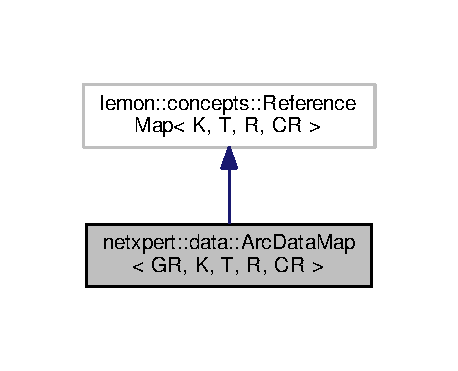
\includegraphics[width=220pt]{classnetxpert_1_1data_1_1ArcDataMap__inherit__graph}
\end{center}
\end{figure}


Collaboration diagram for netxpert\+:\+:data\+:\+:Arc\+Data\+Map$<$ GR, K, T, R, CR $>$\+:\nopagebreak
\begin{figure}[H]
\begin{center}
\leavevmode
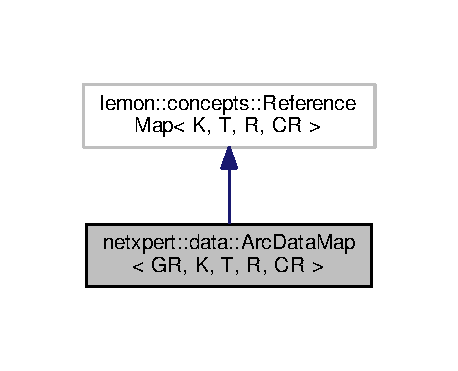
\includegraphics[width=220pt]{classnetxpert_1_1data_1_1ArcDataMap__coll__graph}
\end{center}
\end{figure}
\subsection*{Public Member Functions}
\begin{DoxyCompactItemize}
\item 
\hyperlink{classnetxpert_1_1data_1_1ArcDataMap_a6dd73f6c194b7b4f41a2d3457e90ccb3}{Arc\+Data\+Map} (const GR \&\+\_\+g)
\item 
Reference {\bfseries operator\mbox{[}$\,$\mbox{]}} (const Key \&e)\hypertarget{classnetxpert_1_1data_1_1ArcDataMap_ab19b12bb1dbcc25a57c6b12d7f4bf1f1}{}\label{classnetxpert_1_1data_1_1ArcDataMap_ab19b12bb1dbcc25a57c6b12d7f4bf1f1}

\item 
Const\+Reference {\bfseries operator\mbox{[}$\,$\mbox{]}} (const Key \&e) const \hypertarget{classnetxpert_1_1data_1_1ArcDataMap_a75fd10dc00b5dab7b2545f18af2b18e8}{}\label{classnetxpert_1_1data_1_1ArcDataMap_a75fd10dc00b5dab7b2545f18af2b18e8}

\item 
void {\bfseries set} (const Key \&k, const Value \&v)\hypertarget{classnetxpert_1_1data_1_1ArcDataMap_abed56a049ad56a8fefa45631407cb5f7}{}\label{classnetxpert_1_1data_1_1ArcDataMap_abed56a049ad56a8fefa45631407cb5f7}

\item 
void \hyperlink{classnetxpert_1_1data_1_1ArcDataMap_a2e1260a6420e1d3d12e37a2d419dc51a}{fill\+Cost\+Map} (graph\+\_\+t\+::\+Arc\+Map$<$ cost\+\_\+t $>$ \&\+\_\+cost\+Map)\hypertarget{classnetxpert_1_1data_1_1ArcDataMap_a2e1260a6420e1d3d12e37a2d419dc51a}{}\label{classnetxpert_1_1data_1_1ArcDataMap_a2e1260a6420e1d3d12e37a2d419dc51a}

\begin{DoxyCompactList}\small\item\em fills the cost map that is passed in by reference \end{DoxyCompactList}\item 
void \hyperlink{classnetxpert_1_1data_1_1ArcDataMap_a2b7867df35bee63d8e422a0009ed7a98}{fill\+Cap\+Map} (graph\+\_\+t\+::\+Arc\+Map$<$ capacity\+\_\+t $>$ \&\+\_\+cap\+Map)\hypertarget{classnetxpert_1_1data_1_1ArcDataMap_a2b7867df35bee63d8e422a0009ed7a98}{}\label{classnetxpert_1_1data_1_1ArcDataMap_a2b7867df35bee63d8e422a0009ed7a98}

\begin{DoxyCompactList}\small\item\em fills the capacity map that is passed in by reference \end{DoxyCompactList}\item 
const cost\+\_\+t \hyperlink{classnetxpert_1_1data_1_1ArcDataMap_ab38aa26b69f85d1c03afd8f8ec996328}{get\+Cost} (const Key \&e) const \hypertarget{classnetxpert_1_1data_1_1ArcDataMap_ab38aa26b69f85d1c03afd8f8ec996328}{}\label{classnetxpert_1_1data_1_1ArcDataMap_ab38aa26b69f85d1c03afd8f8ec996328}

\begin{DoxyCompactList}\small\item\em gets the cost for given arc \end{DoxyCompactList}\item 
const capacity\+\_\+t \hyperlink{classnetxpert_1_1data_1_1ArcDataMap_ad61cc93ecab71a5628b5f4669a658d9c}{get\+Cap} (const Key \&e) const \hypertarget{classnetxpert_1_1data_1_1ArcDataMap_ad61cc93ecab71a5628b5f4669a658d9c}{}\label{classnetxpert_1_1data_1_1ArcDataMap_ad61cc93ecab71a5628b5f4669a658d9c}

\begin{DoxyCompactList}\small\item\em gets the cost for given arc \end{DoxyCompactList}\end{DoxyCompactItemize}


\subsection{Detailed Description}
\subsubsection*{template$<$typename GR, typename K, typename T, typename R = T\&, typename CR = const T\&$>$\\*
class netxpert\+::data\+::\+Arc\+Data\+Map$<$ G\+R, K, T, R, C\+R $>$}

Combined structure of graph attribtues as L\+E\+M\+ON Reference Map. 

\begin{DoxyWarning}{Warning}
Not used! 
\end{DoxyWarning}


\subsection{Constructor \& Destructor Documentation}
\index{netxpert\+::data\+::\+Arc\+Data\+Map@{netxpert\+::data\+::\+Arc\+Data\+Map}!Arc\+Data\+Map@{Arc\+Data\+Map}}
\index{Arc\+Data\+Map@{Arc\+Data\+Map}!netxpert\+::data\+::\+Arc\+Data\+Map@{netxpert\+::data\+::\+Arc\+Data\+Map}}
\subsubsection[{\texorpdfstring{Arc\+Data\+Map(const G\+R \&\+\_\+g)}{ArcDataMap(const GR &_g)}}]{\setlength{\rightskip}{0pt plus 5cm}template$<$typename GR , typename K , typename T , typename R  = T\&, typename CR  = const T\&$>$ {\bf netxpert\+::data\+::\+Arc\+Data\+Map}$<$ GR, K, T, R, CR $>$\+::{\bf Arc\+Data\+Map} (
\begin{DoxyParamCaption}
\item[{const GR \&}]{\+\_\+g}
\end{DoxyParamCaption}
)\hspace{0.3cm}{\ttfamily [inline]}}\hypertarget{classnetxpert_1_1data_1_1ArcDataMap_a6dd73f6c194b7b4f41a2d3457e90ccb3}{}\label{classnetxpert_1_1data_1_1ArcDataMap_a6dd73f6c194b7b4f41a2d3457e90ccb3}
Constructor initialize map \char`\"{}\+\_\+data\char`\"{} on construction 

The documentation for this class was generated from the following file\+:\begin{DoxyCompactItemize}
\item 
/home/hahne/dev/netxpert1\+\_\+0/include/lemon-\/net.\+h\end{DoxyCompactItemize}

\hypertarget{classClass}{}\section{Class Class Reference}
\label{classClass}\index{Class@{Class}}


\subsection{Detailed Description}
configuration file for Net\+Xpert 

The documentation for this class was generated from the following file\+:\begin{DoxyCompactItemize}
\item 
/home/hahne/dev/netxpert1\+\_\+0/include/config.\+h\end{DoxyCompactItemize}

\hypertarget{structnetxpert_1_1data_1_1ColumnMap}{}\section{netxpert\+:\+:data\+:\+:Column\+Map Struct Reference}
\label{structnetxpert_1_1data_1_1ColumnMap}\index{netxpert\+::data\+::\+Column\+Map@{netxpert\+::data\+::\+Column\+Map}}


Stores the column names of the input data.  




{\ttfamily \#include $<$data.\+h$>$}

\subsection*{Public Attributes}
\begin{DoxyCompactItemize}
\item 
std\+::string \hyperlink{structnetxpert_1_1data_1_1ColumnMap_afa2e07c5ca6f7bca12dd69aa0f6afb3d}{arc\+I\+D\+Col\+Name}\hypertarget{structnetxpert_1_1data_1_1ColumnMap_afa2e07c5ca6f7bca12dd69aa0f6afb3d}{}\label{structnetxpert_1_1data_1_1ColumnMap_afa2e07c5ca6f7bca12dd69aa0f6afb3d}

\begin{DoxyCompactList}\small\item\em ID column name of the arcs. \end{DoxyCompactList}\item 
std\+::string \hyperlink{structnetxpert_1_1data_1_1ColumnMap_a006100a7e43d78db1fe67277bd2a7363}{from\+Col\+Name}\hypertarget{structnetxpert_1_1data_1_1ColumnMap_a006100a7e43d78db1fe67277bd2a7363}{}\label{structnetxpert_1_1data_1_1ColumnMap_a006100a7e43d78db1fe67277bd2a7363}

\begin{DoxyCompactList}\small\item\em From node column Name of the arcs. \end{DoxyCompactList}\item 
std\+::string \hyperlink{structnetxpert_1_1data_1_1ColumnMap_aae1750eea68bc1f4a7da4d61a6ef9849}{to\+Col\+Name}\hypertarget{structnetxpert_1_1data_1_1ColumnMap_aae1750eea68bc1f4a7da4d61a6ef9849}{}\label{structnetxpert_1_1data_1_1ColumnMap_aae1750eea68bc1f4a7da4d61a6ef9849}

\begin{DoxyCompactList}\small\item\em To node column Name of the arcs. \end{DoxyCompactList}\item 
std\+::string \hyperlink{structnetxpert_1_1data_1_1ColumnMap_a33a2ae88decf47649144469e5209a1c6}{cost\+Col\+Name}\hypertarget{structnetxpert_1_1data_1_1ColumnMap_a33a2ae88decf47649144469e5209a1c6}{}\label{structnetxpert_1_1data_1_1ColumnMap_a33a2ae88decf47649144469e5209a1c6}

\begin{DoxyCompactList}\small\item\em Cost column Name of the arcs. \end{DoxyCompactList}\item 
std\+::string \hyperlink{structnetxpert_1_1data_1_1ColumnMap_af653e17931c6f940746a62db17c1e3a3}{cap\+Col\+Name}\hypertarget{structnetxpert_1_1data_1_1ColumnMap_af653e17931c6f940746a62db17c1e3a3}{}\label{structnetxpert_1_1data_1_1ColumnMap_af653e17931c6f940746a62db17c1e3a3}

\begin{DoxyCompactList}\small\item\em Capacity node column Name of the arcs. \end{DoxyCompactList}\item 
std\+::string \hyperlink{structnetxpert_1_1data_1_1ColumnMap_a46b8b3dbb48282803f1e8b0f53122ecd}{oneway\+Col\+Name}\hypertarget{structnetxpert_1_1data_1_1ColumnMap_a46b8b3dbb48282803f1e8b0f53122ecd}{}\label{structnetxpert_1_1data_1_1ColumnMap_a46b8b3dbb48282803f1e8b0f53122ecd}

\begin{DoxyCompactList}\small\item\em Oneway column Name of the arcs. \end{DoxyCompactList}\item 
std\+::string \hyperlink{structnetxpert_1_1data_1_1ColumnMap_ab1fb1b720e96e33003e3d77179fd870b}{node\+I\+D\+Col\+Name}\hypertarget{structnetxpert_1_1data_1_1ColumnMap_ab1fb1b720e96e33003e3d77179fd870b}{}\label{structnetxpert_1_1data_1_1ColumnMap_ab1fb1b720e96e33003e3d77179fd870b}

\begin{DoxyCompactList}\small\item\em ID column name of the nodes. \end{DoxyCompactList}\item 
std\+::string \hyperlink{structnetxpert_1_1data_1_1ColumnMap_af914fcd7bd73d3f4b678d26d5ac8b586}{supply\+Col\+Name}\hypertarget{structnetxpert_1_1data_1_1ColumnMap_af914fcd7bd73d3f4b678d26d5ac8b586}{}\label{structnetxpert_1_1data_1_1ColumnMap_af914fcd7bd73d3f4b678d26d5ac8b586}

\begin{DoxyCompactList}\small\item\em Supply column name of the nodes. \end{DoxyCompactList}\end{DoxyCompactItemize}


\subsection{Detailed Description}
Stores the column names of the input data. 

The documentation for this struct was generated from the following file\+:\begin{DoxyCompactItemize}
\item 
/home/hahne/dev/netxpert1\+\_\+0/include/data.\+h\end{DoxyCompactItemize}

\hypertarget{structnetxpert_1_1cnfg_1_1Config}{}\section{netxpert\+:\+:cnfg\+:\+:Config Struct Reference}
\label{structnetxpert_1_1cnfg_1_1Config}\index{netxpert\+::cnfg\+::\+Config@{netxpert\+::cnfg\+::\+Config}}


Storage for the configuration of Net\+Xpert.  




{\ttfamily \#include $<$config.\+h$>$}

\subsection*{Public Member Functions}
\begin{DoxyCompactItemize}
\item 
{\footnotesize template$<$class Archive $>$ }\\void \hyperlink{structnetxpert_1_1cnfg_1_1Config_a69a9e3cd168b240c34cfb544c614ebbc}{serialize} (Archive \&ar)
\end{DoxyCompactItemize}
\subsection*{Public Attributes}
\begin{DoxyCompactItemize}
\item 
std\+::string \hyperlink{structnetxpert_1_1cnfg_1_1Config_abfbfd2126c7d8e675f1c786cf7a1004a}{Net\+X\+D\+B\+Path}\hypertarget{structnetxpert_1_1cnfg_1_1Config_abfbfd2126c7d8e675f1c786cf7a1004a}{}\label{structnetxpert_1_1cnfg_1_1Config_abfbfd2126c7d8e675f1c786cf7a1004a}

\begin{DoxyCompactList}\small\item\em Path for the input database. \end{DoxyCompactList}\item 
std\+::string \hyperlink{structnetxpert_1_1cnfg_1_1Config_a11f88b978f21663025714bff816cfe86}{Result\+D\+B\+Path}\hypertarget{structnetxpert_1_1cnfg_1_1Config_a11f88b978f21663025714bff816cfe86}{}\label{structnetxpert_1_1cnfg_1_1Config_a11f88b978f21663025714bff816cfe86}

\begin{DoxyCompactList}\small\item\em Path for the result database. \end{DoxyCompactList}\item 
\hyperlink{namespacenetxpert_1_1cnfg_a235b32f52360f5f331279b34e85064a5}{netxpert\+::cnfg\+::\+R\+E\+S\+U\+L\+T\+\_\+\+D\+B\+\_\+\+T\+Y\+PE} \hyperlink{structnetxpert_1_1cnfg_1_1Config_a088abe76a5f5b531b7294122b1a63542}{Result\+D\+B\+Type}\hypertarget{structnetxpert_1_1cnfg_1_1Config_a088abe76a5f5b531b7294122b1a63542}{}\label{structnetxpert_1_1cnfg_1_1Config_a088abe76a5f5b531b7294122b1a63542}

\begin{DoxyCompactList}\small\item\em Type of the result database type. \end{DoxyCompactList}\item 
std\+::string \hyperlink{structnetxpert_1_1cnfg_1_1Config_a365d31191baf6a1bc7b700e949c1ac05}{Result\+Table\+Name}\hypertarget{structnetxpert_1_1cnfg_1_1Config_a365d31191baf6a1bc7b700e949c1ac05}{}\label{structnetxpert_1_1cnfg_1_1Config_a365d31191baf6a1bc7b700e949c1ac05}

\begin{DoxyCompactList}\small\item\em Name of the result table. \end{DoxyCompactList}\item 
bool \hyperlink{structnetxpert_1_1cnfg_1_1Config_a899d7ea93cedfb52addfd6ba9dc23ef8}{S\+P\+T\+All\+Dests}\hypertarget{structnetxpert_1_1cnfg_1_1Config_a899d7ea93cedfb52addfd6ba9dc23ef8}{}\label{structnetxpert_1_1cnfg_1_1Config_a899d7ea93cedfb52addfd6ba9dc23ef8}

\begin{DoxyCompactList}\small\item\em If true, then all shortest paths from the given start point to all reachable destinations in the network will be computed in the shortest path solver. \end{DoxyCompactList}\item 
int \hyperlink{structnetxpert_1_1cnfg_1_1Config_a41afc9fb4f15155eec2f8c30eaae5500}{S\+P\+T\+Heap\+Card}
\begin{DoxyCompactList}\small\item\em Ariety for the heap structure in shortest path algorithms if supported. \end{DoxyCompactList}\item 
\hyperlink{namespacenetxpert_1_1cnfg_a6ff755ed7f76e0049e3eeeed86c9b55d}{netxpert\+::cnfg\+::\+S\+P\+T\+Algorithm} \hyperlink{structnetxpert_1_1cnfg_1_1Config_a207a8bc8efda8c4c67a256a13ed54e05}{Spt\+Algorithm}\hypertarget{structnetxpert_1_1cnfg_1_1Config_a207a8bc8efda8c4c67a256a13ed54e05}{}\label{structnetxpert_1_1cnfg_1_1Config_a207a8bc8efda8c4c67a256a13ed54e05}

\begin{DoxyCompactList}\small\item\em Shortest path algorithm to use. \end{DoxyCompactList}\item 
\hyperlink{namespacenetxpert_1_1cnfg_aae922390a89b0c9af1bc2532428c5ef9}{netxpert\+::cnfg\+::\+M\+C\+F\+Algorithm} \hyperlink{structnetxpert_1_1cnfg_1_1Config_af33b0b153b4682b2cff31be437acd0c1}{Mcf\+Algorithm}\hypertarget{structnetxpert_1_1cnfg_1_1Config_af33b0b153b4682b2cff31be437acd0c1}{}\label{structnetxpert_1_1cnfg_1_1Config_af33b0b153b4682b2cff31be437acd0c1}

\begin{DoxyCompactList}\small\item\em Minimum cost flow algorithm to use. \end{DoxyCompactList}\item 
\hyperlink{namespacenetxpert_1_1cnfg_ab77ff30f2da32945dbb19bdf6199f799}{netxpert\+::cnfg\+::\+M\+S\+T\+Algorithm} \hyperlink{structnetxpert_1_1cnfg_1_1Config_a7d4b58830190d9c7d79b23a61625bd44}{Mst\+Algorithm}\hypertarget{structnetxpert_1_1cnfg_1_1Config_a7d4b58830190d9c7d79b23a61625bd44}{}\label{structnetxpert_1_1cnfg_1_1Config_a7d4b58830190d9c7d79b23a61625bd44}

\begin{DoxyCompactList}\small\item\em Minimum spanning tree algorithm to use. \end{DoxyCompactList}\item 
bool \hyperlink{structnetxpert_1_1cnfg_1_1Config_a732e585e5f3cf8e04c7b230fd0b9aaf5}{Is\+Directed}\hypertarget{structnetxpert_1_1cnfg_1_1Config_a732e585e5f3cf8e04c7b230fd0b9aaf5}{}\label{structnetxpert_1_1cnfg_1_1Config_a732e585e5f3cf8e04c7b230fd0b9aaf5}

\begin{DoxyCompactList}\small\item\em Network is directed or bidirectional. \end{DoxyCompactList}\item 
std\+::string \hyperlink{structnetxpert_1_1cnfg_1_1Config_a123bb51f96e9136786cda1256b6ba68b}{Arcs\+Table\+Name}\hypertarget{structnetxpert_1_1cnfg_1_1Config_a123bb51f96e9136786cda1256b6ba68b}{}\label{structnetxpert_1_1cnfg_1_1Config_a123bb51f96e9136786cda1256b6ba68b}

\begin{DoxyCompactList}\small\item\em Name of the input arcs table. \end{DoxyCompactList}\item 
std\+::string \hyperlink{structnetxpert_1_1cnfg_1_1Config_aad2f1620e6f0724d682e8b789a3e5f84}{Arcs\+Geom\+Column\+Name}\hypertarget{structnetxpert_1_1cnfg_1_1Config_aad2f1620e6f0724d682e8b789a3e5f84}{}\label{structnetxpert_1_1cnfg_1_1Config_aad2f1620e6f0724d682e8b789a3e5f84}

\begin{DoxyCompactList}\small\item\em Geometry column name of the input arcs table. \end{DoxyCompactList}\item 
std\+::string \hyperlink{structnetxpert_1_1cnfg_1_1Config_a9c2df9c1f47014aef22ebd85e227907c}{Arc\+I\+D\+Column\+Name}\hypertarget{structnetxpert_1_1cnfg_1_1Config_a9c2df9c1f47014aef22ebd85e227907c}{}\label{structnetxpert_1_1cnfg_1_1Config_a9c2df9c1f47014aef22ebd85e227907c}

\begin{DoxyCompactList}\small\item\em ID column name of the input arcs table. \end{DoxyCompactList}\item 
std\+::string \hyperlink{structnetxpert_1_1cnfg_1_1Config_a7751fdb84c5fb76f8af07dba25768357}{From\+Node\+Column\+Name}\hypertarget{structnetxpert_1_1cnfg_1_1Config_a7751fdb84c5fb76f8af07dba25768357}{}\label{structnetxpert_1_1cnfg_1_1Config_a7751fdb84c5fb76f8af07dba25768357}

\begin{DoxyCompactList}\small\item\em From node column name of the input arcs table. \end{DoxyCompactList}\item 
std\+::string \hyperlink{structnetxpert_1_1cnfg_1_1Config_af5ab8e729eafee4eb059a251343d68f8}{To\+Node\+Column\+Name}\hypertarget{structnetxpert_1_1cnfg_1_1Config_af5ab8e729eafee4eb059a251343d68f8}{}\label{structnetxpert_1_1cnfg_1_1Config_af5ab8e729eafee4eb059a251343d68f8}

\begin{DoxyCompactList}\small\item\em To node column name of the input arcs table. \end{DoxyCompactList}\item 
std\+::string \hyperlink{structnetxpert_1_1cnfg_1_1Config_ac7b02cb4adb2b72140f73ab97f76fad8}{Cost\+Column\+Name}\hypertarget{structnetxpert_1_1cnfg_1_1Config_ac7b02cb4adb2b72140f73ab97f76fad8}{}\label{structnetxpert_1_1cnfg_1_1Config_ac7b02cb4adb2b72140f73ab97f76fad8}

\begin{DoxyCompactList}\small\item\em Cost column name of the input arcs table. \end{DoxyCompactList}\item 
std\+::string \hyperlink{structnetxpert_1_1cnfg_1_1Config_a2587718329c1c79ac894c48793202e4f}{Cap\+Column\+Name}\hypertarget{structnetxpert_1_1cnfg_1_1Config_a2587718329c1c79ac894c48793202e4f}{}\label{structnetxpert_1_1cnfg_1_1Config_a2587718329c1c79ac894c48793202e4f}

\begin{DoxyCompactList}\small\item\em Capacity column name of the input arcs table. \end{DoxyCompactList}\item 
std\+::string \hyperlink{structnetxpert_1_1cnfg_1_1Config_a89556dbbbadcfbd6055346a4ad77e353}{Oneway\+Column\+Name}\hypertarget{structnetxpert_1_1cnfg_1_1Config_a89556dbbbadcfbd6055346a4ad77e353}{}\label{structnetxpert_1_1cnfg_1_1Config_a89556dbbbadcfbd6055346a4ad77e353}

\begin{DoxyCompactList}\small\item\em Oneway column name of the input arcs table. \end{DoxyCompactList}\item 
std\+::string \hyperlink{structnetxpert_1_1cnfg_1_1Config_a3bc097716fc6afe10d3c96b35edeb83a}{Nodes\+Table\+Name}\hypertarget{structnetxpert_1_1cnfg_1_1Config_a3bc097716fc6afe10d3c96b35edeb83a}{}\label{structnetxpert_1_1cnfg_1_1Config_a3bc097716fc6afe10d3c96b35edeb83a}

\begin{DoxyCompactList}\small\item\em Name of the input nodes table. \end{DoxyCompactList}\item 
std\+::string \hyperlink{structnetxpert_1_1cnfg_1_1Config_a9c7263b8431c13be4187e4451baae541}{Nodes\+Geom\+Column\+Name}\hypertarget{structnetxpert_1_1cnfg_1_1Config_a9c7263b8431c13be4187e4451baae541}{}\label{structnetxpert_1_1cnfg_1_1Config_a9c7263b8431c13be4187e4451baae541}

\begin{DoxyCompactList}\small\item\em Geometry column name of the input nodes table. \end{DoxyCompactList}\item 
std\+::string \hyperlink{structnetxpert_1_1cnfg_1_1Config_a1faa14bece3cacb0366586674ce177e7}{Node\+I\+D\+Column\+Name}\hypertarget{structnetxpert_1_1cnfg_1_1Config_a1faa14bece3cacb0366586674ce177e7}{}\label{structnetxpert_1_1cnfg_1_1Config_a1faa14bece3cacb0366586674ce177e7}

\begin{DoxyCompactList}\small\item\em ID column name of the input nodes table. \end{DoxyCompactList}\item 
std\+::string \hyperlink{structnetxpert_1_1cnfg_1_1Config_a27ffb6532db544982eda53d2b3aad656}{Node\+Supply\+Column\+Name}\hypertarget{structnetxpert_1_1cnfg_1_1Config_a27ffb6532db544982eda53d2b3aad656}{}\label{structnetxpert_1_1cnfg_1_1Config_a27ffb6532db544982eda53d2b3aad656}

\begin{DoxyCompactList}\small\item\em Supply column name of the input nodes table. \end{DoxyCompactList}\item 
std\+::string \hyperlink{structnetxpert_1_1cnfg_1_1Config_aa30fa621c656cc1fb53dc7f32a122426}{Barrier\+Poly\+Table\+Name}\hypertarget{structnetxpert_1_1cnfg_1_1Config_aa30fa621c656cc1fb53dc7f32a122426}{}\label{structnetxpert_1_1cnfg_1_1Config_aa30fa621c656cc1fb53dc7f32a122426}

\begin{DoxyCompactList}\small\item\em Name of the barrier polygon table. \end{DoxyCompactList}\item 
std\+::string \hyperlink{structnetxpert_1_1cnfg_1_1Config_ad4dcf3083176c2c7dfdde577cef9b5d9}{Barrier\+Poly\+Geom\+Column\+Name}\hypertarget{structnetxpert_1_1cnfg_1_1Config_ad4dcf3083176c2c7dfdde577cef9b5d9}{}\label{structnetxpert_1_1cnfg_1_1Config_ad4dcf3083176c2c7dfdde577cef9b5d9}

\begin{DoxyCompactList}\small\item\em Geometry column name of the barrier polygon table. \end{DoxyCompactList}\item 
std\+::string \hyperlink{structnetxpert_1_1cnfg_1_1Config_aa352c00d9f5796d2ff964b1982f5f35d}{Barrier\+Line\+Table\+Name}\hypertarget{structnetxpert_1_1cnfg_1_1Config_aa352c00d9f5796d2ff964b1982f5f35d}{}\label{structnetxpert_1_1cnfg_1_1Config_aa352c00d9f5796d2ff964b1982f5f35d}

\begin{DoxyCompactList}\small\item\em Name of the barrier line table. \end{DoxyCompactList}\item 
std\+::string \hyperlink{structnetxpert_1_1cnfg_1_1Config_a53c92c5975dbb9b861f87838021c360e}{Barrier\+Line\+Geom\+Column\+Name}\hypertarget{structnetxpert_1_1cnfg_1_1Config_a53c92c5975dbb9b861f87838021c360e}{}\label{structnetxpert_1_1cnfg_1_1Config_a53c92c5975dbb9b861f87838021c360e}

\begin{DoxyCompactList}\small\item\em Geometry column name of the barrier line table. \end{DoxyCompactList}\item 
std\+::string \hyperlink{structnetxpert_1_1cnfg_1_1Config_a344e11f497239a95bb1cf7f94542dcbc}{Barrier\+Point\+Table\+Name}\hypertarget{structnetxpert_1_1cnfg_1_1Config_a344e11f497239a95bb1cf7f94542dcbc}{}\label{structnetxpert_1_1cnfg_1_1Config_a344e11f497239a95bb1cf7f94542dcbc}

\begin{DoxyCompactList}\small\item\em Name of the barrier point table. \end{DoxyCompactList}\item 
std\+::string \hyperlink{structnetxpert_1_1cnfg_1_1Config_ad4ab91f16c00fba3b04c76ba770e80e1}{Barrier\+Point\+Geom\+Column\+Name}\hypertarget{structnetxpert_1_1cnfg_1_1Config_ad4ab91f16c00fba3b04c76ba770e80e1}{}\label{structnetxpert_1_1cnfg_1_1Config_ad4ab91f16c00fba3b04c76ba770e80e1}

\begin{DoxyCompactList}\small\item\em Geometry column name of the barrier point table. \end{DoxyCompactList}\item 
int \hyperlink{structnetxpert_1_1cnfg_1_1Config_aee1dee4ec74c14f60bbb87c3c267255f}{Treshold}\hypertarget{structnetxpert_1_1cnfg_1_1Config_aee1dee4ec74c14f60bbb87c3c267255f}{}\label{structnetxpert_1_1cnfg_1_1Config_aee1dee4ec74c14f60bbb87c3c267255f}

\begin{DoxyCompactList}\small\item\em Treshold for distance search\+: closest arc of network to given point; (Snapping tolerance) \end{DoxyCompactList}\item 
bool \hyperlink{structnetxpert_1_1cnfg_1_1Config_a415b76b1b41d24dc3b4cf11b9021f366}{Use\+Spatial\+Index}
\item 
bool \hyperlink{structnetxpert_1_1cnfg_1_1Config_ac94abe7cd836323220db9e8f7ac674df}{Load\+D\+B\+Into\+Memory}
\item 
int \hyperlink{structnetxpert_1_1cnfg_1_1Config_a56651fcf68e1afe6d0a9b042301508ed}{Number\+Of\+Tests}\hypertarget{structnetxpert_1_1cnfg_1_1Config_a56651fcf68e1afe6d0a9b042301508ed}{}\label{structnetxpert_1_1cnfg_1_1Config_a56651fcf68e1afe6d0a9b042301508ed}

\begin{DoxyCompactList}\small\item\em Number of tests to run. \end{DoxyCompactList}\item 
std\+::string \hyperlink{structnetxpert_1_1cnfg_1_1Config_a30e9c138aaee454b4b9f178a5d9fec0a}{Spatia\+Lite\+Home}\hypertarget{structnetxpert_1_1cnfg_1_1Config_a30e9c138aaee454b4b9f178a5d9fec0a}{}\label{structnetxpert_1_1cnfg_1_1Config_a30e9c138aaee454b4b9f178a5d9fec0a}

\begin{DoxyCompactList}\small\item\em Path to the directory of the Spatia\+Lite library. \end{DoxyCompactList}\item 
std\+::string \hyperlink{structnetxpert_1_1cnfg_1_1Config_a4df2574cae792012d65db17eaf3d0a22}{Spatia\+Lite\+Core\+Name}\hypertarget{structnetxpert_1_1cnfg_1_1Config_a4df2574cae792012d65db17eaf3d0a22}{}\label{structnetxpert_1_1cnfg_1_1Config_a4df2574cae792012d65db17eaf3d0a22}

\begin{DoxyCompactList}\small\item\em Name of the Spatia\+Lite library (without file extension) \end{DoxyCompactList}\item 
\hyperlink{namespacenetxpert_1_1cnfg_a1514d3ae51414bf0bcd8d1fe8e868b89}{netxpert\+::cnfg\+::\+G\+E\+O\+M\+E\+T\+R\+Y\+\_\+\+H\+A\+N\+D\+L\+I\+NG} \hyperlink{structnetxpert_1_1cnfg_1_1Config_abad7200444a8c97b59bc6978a7abeae6}{Geometry\+Handling}\hypertarget{structnetxpert_1_1cnfg_1_1Config_abad7200444a8c97b59bc6978a7abeae6}{}\label{structnetxpert_1_1cnfg_1_1Config_abad7200444a8c97b59bc6978a7abeae6}

\begin{DoxyCompactList}\small\item\em Geometry handling (no geometry, straight lines, real geometry). \end{DoxyCompactList}\item 
\hyperlink{namespacenetxpert_1_1cnfg_ae473d83baf6d2ee9328c66364eefc8df}{netxpert\+::cnfg\+::\+T\+E\+S\+T\+C\+A\+SE} \hyperlink{structnetxpert_1_1cnfg_1_1Config_a73f9299fb8e35e1f4a9946f37dc3d17c}{Test\+Case}\hypertarget{structnetxpert_1_1cnfg_1_1Config_a73f9299fb8e35e1f4a9946f37dc3d17c}{}\label{structnetxpert_1_1cnfg_1_1Config_a73f9299fb8e35e1f4a9946f37dc3d17c}

\begin{DoxyCompactList}\small\item\em Test case to run. \end{DoxyCompactList}\item 
\hyperlink{namespacenetxpert_1_1cnfg_ac9cb46108300f2d88ac15f7460ca0696}{netxpert\+::cnfg\+::\+L\+O\+G\+\_\+\+L\+E\+V\+EL} \hyperlink{structnetxpert_1_1cnfg_1_1Config_a41d9e5a7901723efc1afb53384a42826}{Log\+Level}\hypertarget{structnetxpert_1_1cnfg_1_1Config_a41d9e5a7901723efc1afb53384a42826}{}\label{structnetxpert_1_1cnfg_1_1Config_a41d9e5a7901723efc1afb53384a42826}

\begin{DoxyCompactList}\small\item\em Application log level. \end{DoxyCompactList}\item 
bool \hyperlink{structnetxpert_1_1cnfg_1_1Config_aef1cbd3c83c99e7cb677594ef154fa3f}{Clean\+Network}\hypertarget{structnetxpert_1_1cnfg_1_1Config_aef1cbd3c83c99e7cb677594ef154fa3f}{}\label{structnetxpert_1_1cnfg_1_1Config_aef1cbd3c83c99e7cb677594ef154fa3f}

\begin{DoxyCompactList}\small\item\em Clean input network on load. \end{DoxyCompactList}\item 
std\+::string \hyperlink{structnetxpert_1_1cnfg_1_1Config_a32bdb3e794544e30465de6224a9f92bb}{Log\+File\+Full\+Path}\hypertarget{structnetxpert_1_1cnfg_1_1Config_a32bdb3e794544e30465de6224a9f92bb}{}\label{structnetxpert_1_1cnfg_1_1Config_a32bdb3e794544e30465de6224a9f92bb}

\begin{DoxyCompactList}\small\item\em Path to log file. \end{DoxyCompactList}\end{DoxyCompactItemize}


\subsection{Detailed Description}
Storage for the configuration of Net\+Xpert. 

\subsection{Member Function Documentation}
\index{netxpert\+::cnfg\+::\+Config@{netxpert\+::cnfg\+::\+Config}!serialize@{serialize}}
\index{serialize@{serialize}!netxpert\+::cnfg\+::\+Config@{netxpert\+::cnfg\+::\+Config}}
\subsubsection[{\texorpdfstring{serialize(\+Archive \&ar)}{serialize(Archive &ar)}}]{\setlength{\rightskip}{0pt plus 5cm}template$<$class Archive $>$ void netxpert\+::cnfg\+::\+Config\+::serialize (
\begin{DoxyParamCaption}
\item[{Archive \&}]{ar}
\end{DoxyParamCaption}
)\hspace{0.3cm}{\ttfamily [inline]}}\hypertarget{structnetxpert_1_1cnfg_1_1Config_a69a9e3cd168b240c34cfb544c614ebbc}{}\label{structnetxpert_1_1cnfg_1_1Config_a69a9e3cd168b240c34cfb544c614ebbc}
Serialize struct members to json 

\subsection{Member Data Documentation}
\index{netxpert\+::cnfg\+::\+Config@{netxpert\+::cnfg\+::\+Config}!Load\+D\+B\+Into\+Memory@{Load\+D\+B\+Into\+Memory}}
\index{Load\+D\+B\+Into\+Memory@{Load\+D\+B\+Into\+Memory}!netxpert\+::cnfg\+::\+Config@{netxpert\+::cnfg\+::\+Config}}
\subsubsection[{\texorpdfstring{Load\+D\+B\+Into\+Memory}{LoadDBIntoMemory}}]{\setlength{\rightskip}{0pt plus 5cm}bool netxpert\+::cnfg\+::\+Config\+::\+Load\+D\+B\+Into\+Memory}\hypertarget{structnetxpert_1_1cnfg_1_1Config_ac94abe7cd836323220db9e8f7ac674df}{}\label{structnetxpert_1_1cnfg_1_1Config_ac94abe7cd836323220db9e8f7ac674df}
\begin{DoxyRefDesc}{Deprecated}
\item[\hyperlink{deprecated__deprecated000002}{Deprecated}]Load input database into memory. \end{DoxyRefDesc}
\index{netxpert\+::cnfg\+::\+Config@{netxpert\+::cnfg\+::\+Config}!S\+P\+T\+Heap\+Card@{S\+P\+T\+Heap\+Card}}
\index{S\+P\+T\+Heap\+Card@{S\+P\+T\+Heap\+Card}!netxpert\+::cnfg\+::\+Config@{netxpert\+::cnfg\+::\+Config}}
\subsubsection[{\texorpdfstring{S\+P\+T\+Heap\+Card}{SPTHeapCard}}]{\setlength{\rightskip}{0pt plus 5cm}int netxpert\+::cnfg\+::\+Config\+::\+S\+P\+T\+Heap\+Card}\hypertarget{structnetxpert_1_1cnfg_1_1Config_a41afc9fb4f15155eec2f8c30eaae5500}{}\label{structnetxpert_1_1cnfg_1_1Config_a41afc9fb4f15155eec2f8c30eaae5500}


Ariety for the heap structure in shortest path algorithms if supported. 

\begin{DoxyWarning}{Warning}
Unsed at the moment! 
\end{DoxyWarning}
\index{netxpert\+::cnfg\+::\+Config@{netxpert\+::cnfg\+::\+Config}!Use\+Spatial\+Index@{Use\+Spatial\+Index}}
\index{Use\+Spatial\+Index@{Use\+Spatial\+Index}!netxpert\+::cnfg\+::\+Config@{netxpert\+::cnfg\+::\+Config}}
\subsubsection[{\texorpdfstring{Use\+Spatial\+Index}{UseSpatialIndex}}]{\setlength{\rightskip}{0pt plus 5cm}bool netxpert\+::cnfg\+::\+Config\+::\+Use\+Spatial\+Index}\hypertarget{structnetxpert_1_1cnfg_1_1Config_a415b76b1b41d24dc3b4cf11b9021f366}{}\label{structnetxpert_1_1cnfg_1_1Config_a415b76b1b41d24dc3b4cf11b9021f366}
\begin{DoxyRefDesc}{Deprecated}
\item[\hyperlink{deprecated__deprecated000001}{Deprecated}]Use spatial index or not in input database. Default\+: true \end{DoxyRefDesc}


The documentation for this struct was generated from the following file\+:\begin{DoxyCompactItemize}
\item 
/home/hahne/dev/netxpert1\+\_\+0/include/config.\+h\end{DoxyCompactItemize}

\hypertarget{classnetxpert_1_1cnfg_1_1ConfigReader}{}\section{netxpert\+:\+:cnfg\+:\+:Config\+Reader Class Reference}
\label{classnetxpert_1_1cnfg_1_1ConfigReader}\index{netxpert\+::cnfg\+::\+Config\+Reader@{netxpert\+::cnfg\+::\+Config\+Reader}}
\subsection*{Public Member Functions}
\begin{DoxyCompactItemize}
\item 
\hyperlink{structnetxpert_1_1cnfg_1_1Config}{Config} {\bfseries Get\+Config\+From\+J\+S\+ON} (std\+::string json\+String)\hypertarget{classnetxpert_1_1cnfg_1_1ConfigReader_adb5756de4a36b951ef31e40f6ead49bc}{}\label{classnetxpert_1_1cnfg_1_1ConfigReader_adb5756de4a36b951ef31e40f6ead49bc}

\item 
void {\bfseries Get\+Config\+From\+J\+S\+O\+N\+File} (std\+::string file\+Name, \hyperlink{structnetxpert_1_1cnfg_1_1Config}{netxpert\+::cnfg\+::\+Config} \&cnfg)\hypertarget{classnetxpert_1_1cnfg_1_1ConfigReader_a3752b114bf9de7624eab789c37acdc0f}{}\label{classnetxpert_1_1cnfg_1_1ConfigReader_a3752b114bf9de7624eab789c37acdc0f}

\end{DoxyCompactItemize}


The documentation for this class was generated from the following file\+:\begin{DoxyCompactItemize}
\item 
/home/hahne/dev/netxpert1\+\_\+0/include/config.\+h\end{DoxyCompactItemize}

\hypertarget{classnetxpert_1_1io_1_1DBHELPER}{}\section{netxpert\+:\+:io\+:\+:D\+B\+H\+E\+L\+P\+ER Class Reference}
\label{classnetxpert_1_1io_1_1DBHELPER}\index{netxpert\+::io\+::\+D\+B\+H\+E\+L\+P\+ER@{netxpert\+::io\+::\+D\+B\+H\+E\+L\+P\+ER}}


Static \hyperlink{classClass}{Class} that controls the Spatia\+Lite DB processing access.  




{\ttfamily \#include $<$dbhelper.\+h$>$}

\subsection*{Static Public Member Functions}
\begin{DoxyCompactItemize}
\item 
static void {\bfseries Initialize} (const \hyperlink{structnetxpert_1_1cnfg_1_1Config}{netxpert\+::cnfg\+::\+Config} \&cnfg)\hypertarget{classnetxpert_1_1io_1_1DBHELPER_a091b1da6ebcbb415f633383ce9f3732e}{}\label{classnetxpert_1_1io_1_1DBHELPER_a091b1da6ebcbb415f633383ce9f3732e}

\item 
static void {\bfseries Commit\+Current\+Transaction} ()\hypertarget{classnetxpert_1_1io_1_1DBHELPER_ac6f26d9cd75b7425606193cd94cd8ce0}{}\label{classnetxpert_1_1io_1_1DBHELPER_ac6f26d9cd75b7425606193cd94cd8ce0}

\item 
static void {\bfseries Open\+New\+Transaction} ()\hypertarget{classnetxpert_1_1io_1_1DBHELPER_ab0f5e0871bfe5ccf43eacc467ba1d1e5}{}\label{classnetxpert_1_1io_1_1DBHELPER_ab0f5e0871bfe5ccf43eacc467ba1d1e5}

\item 
static netxpert\+::data\+::\+Input\+Arcs {\bfseries Load\+Network\+From\+DB} (const std\+::string \&\+\_\+table\+Name, const \hyperlink{structnetxpert_1_1data_1_1ColumnMap}{netxpert\+::data\+::\+Column\+Map} \&\+\_\+map)\hypertarget{classnetxpert_1_1io_1_1DBHELPER_adea7317655d98165addf32ca98246e55}{}\label{classnetxpert_1_1io_1_1DBHELPER_adea7317655d98165addf32ca98246e55}

\item 
static netxpert\+::data\+::\+Network\+Builder\+Input\+Arcs {\bfseries Load\+Network\+To\+Build\+From\+DB} (const std\+::string \&\+\_\+table\+Name, const \hyperlink{structnetxpert_1_1data_1_1ColumnMap}{netxpert\+::data\+::\+Column\+Map} \&\+\_\+map)\hypertarget{classnetxpert_1_1io_1_1DBHELPER_ae2938be0a57e275a376ddad51ea0561f}{}\label{classnetxpert_1_1io_1_1DBHELPER_ae2938be0a57e275a376ddad51ea0561f}

\item 
static std\+::vector$<$ \hyperlink{structnetxpert_1_1data_1_1NewNode}{netxpert\+::data\+::\+New\+Node} $>$ {\bfseries Load\+Nodes\+From\+DB} (const std\+::string \&\+\_\+table\+Name, const std\+::string \&geom\+Col\+Name, const \hyperlink{structnetxpert_1_1data_1_1ColumnMap}{netxpert\+::data\+::\+Column\+Map} \&\+\_\+map)\hypertarget{classnetxpert_1_1io_1_1DBHELPER_a81a4919efc4dc8d35bb2ba47ae55da25}{}\label{classnetxpert_1_1io_1_1DBHELPER_a81a4919efc4dc8d35bb2ba47ae55da25}

\item 
static std\+::unique\+\_\+ptr$<$ S\+Q\+Lite\+::\+Statement $>$ {\bfseries Prepare\+Get\+Closest\+Arc\+Query} (const std\+::string \&table\+Name, const std\+::string \&geom\+Column\+Name, const \hyperlink{structnetxpert_1_1data_1_1ColumnMap}{netxpert\+::data\+::\+Column\+Map} \&cmap, const \hyperlink{namespacenetxpert_1_1data_a7f0e5c814a8a55ea94f348b10826e206}{netxpert\+::data\+::\+Arc\+I\+D\+Column\+Data\+Type} arc\+I\+D\+Col\+Data\+Type, const bool with\+Capacity)\hypertarget{classnetxpert_1_1io_1_1DBHELPER_afeea6c99ff55007ab5079c75c39bd4c6}{}\label{classnetxpert_1_1io_1_1DBHELPER_afeea6c99ff55007ab5079c75c39bd4c6}

\item 
static \hyperlink{structnetxpert_1_1data_1_1ExtClosestArcAndPoint}{netxpert\+::data\+::\+Ext\+Closest\+Arc\+And\+Point} {\bfseries Get\+Closest\+Arc\+From\+Point} (const geos\+::geom\+::\+Coordinate \&coord, const int treshold, S\+Q\+Lite\+::\+Statement \&qry, const bool with\+Capacity)\hypertarget{classnetxpert_1_1io_1_1DBHELPER_ae842b4ce30eee6ec2c85444844318994}{}\label{classnetxpert_1_1io_1_1DBHELPER_ae842b4ce30eee6ec2c85444844318994}

\item 
static std\+::unique\+\_\+ptr$<$ geos\+::geom\+::\+Multi\+Line\+String $>$ {\bfseries Get\+Arc\+Geometry\+From\+DB} (const std\+::string \&table\+Name, const std\+::string \&arc\+I\+D\+Column\+Name, const std\+::string \&geom\+Column\+Name, const \hyperlink{namespacenetxpert_1_1data_a7f0e5c814a8a55ea94f348b10826e206}{netxpert\+::data\+::\+Arc\+I\+D\+Column\+Data\+Type} arc\+I\+D\+Col\+Data\+Type, const netxpert\+::data\+::extarcid\+\_\+t \&arc\+ID)\hypertarget{classnetxpert_1_1io_1_1DBHELPER_af44cf45d7c4ee81a3e4037901efeb43f}{}\label{classnetxpert_1_1io_1_1DBHELPER_af44cf45d7c4ee81a3e4037901efeb43f}

\item 
static std\+::unique\+\_\+ptr$<$ geos\+::geom\+::\+Multi\+Line\+String $>$ {\bfseries Get\+Arc\+Geometries\+From\+DB} (const std\+::string \&table\+Name, const std\+::string \&arc\+I\+D\+Column\+Name, const std\+::string \&geom\+Column\+Name, const \hyperlink{namespacenetxpert_1_1data_a7f0e5c814a8a55ea94f348b10826e206}{netxpert\+::data\+::\+Arc\+I\+D\+Column\+Data\+Type} arc\+I\+D\+Col\+Data\+Type, const std\+::string \&arc\+I\+Ds)\hypertarget{classnetxpert_1_1io_1_1DBHELPER_a1e91daf8cd224e722ea58a522c5043e2}{}\label{classnetxpert_1_1io_1_1DBHELPER_a1e91daf8cd224e722ea58a522c5043e2}

\item 
static std\+::unordered\+\_\+set$<$ netxpert\+::data\+::extarcid\+\_\+t $>$ {\bfseries Get\+Intersecting\+Arcs} (const std\+::string \&barrier\+Table\+Name, const std\+::string \&barrier\+Geom\+Col\+Name, const std\+::string \&arcs\+Table\+Name, const std\+::string \&arc\+I\+D\+Col\+Name, const std\+::string \&arc\+Geom\+Col\+Name)\hypertarget{classnetxpert_1_1io_1_1DBHELPER_afdfafd0732ca51ce231422b5372541d4}{}\label{classnetxpert_1_1io_1_1DBHELPER_afdfafd0732ca51ce231422b5372541d4}

\item 
static std\+::vector$<$ std\+::unique\+\_\+ptr$<$ geos\+::geom\+::\+Geometry $>$ $>$ {\bfseries Get\+Barrier\+Geometries\+From\+DB} (const std\+::string \&barrier\+Table\+Name, const std\+::string \&barrier\+Geom\+Col\+Name)\hypertarget{classnetxpert_1_1io_1_1DBHELPER_a03a39530e7e86cfa58a0c7d69bd95b7a}{}\label{classnetxpert_1_1io_1_1DBHELPER_a03a39530e7e86cfa58a0c7d69bd95b7a}

\item 
static std\+::unique\+\_\+ptr$<$ geos\+::geom\+::\+Multi\+Point $>$ {\bfseries Get\+Arc\+Vertex\+Geometries\+By\+Buffer\+From\+DB} (const std\+::string \&table\+Name, const std\+::string \&geom\+Column\+Name, const \hyperlink{namespacenetxpert_1_1data_a7f0e5c814a8a55ea94f348b10826e206}{netxpert\+::data\+::\+Arc\+I\+D\+Column\+Data\+Type} arc\+I\+D\+Col\+Data\+Type, const std\+::string \&arc\+I\+D\+Col\+Name, const double buffer\+Val, const geos\+::geom\+::\+Coordinate \&p)\hypertarget{classnetxpert_1_1io_1_1DBHELPER_af5fea985543faa266073b9584c9c2993}{}\label{classnetxpert_1_1io_1_1DBHELPER_af5fea985543faa266073b9584c9c2993}

\item 
static std\+::unique\+\_\+ptr$<$ S\+Q\+Lite\+::\+Statement $>$ {\bfseries Prepare\+Is\+Point\+On\+Arc\+Query} (std\+::string table\+Name, std\+::string arc\+I\+D\+Column\+Name, std\+::string geom\+Column\+Name, \hyperlink{namespacenetxpert_1_1data_a7f0e5c814a8a55ea94f348b10826e206}{netxpert\+::data\+::\+Arc\+I\+D\+Column\+Data\+Type} arc\+I\+D\+Col\+Data\+Type)\hypertarget{classnetxpert_1_1io_1_1DBHELPER_a9d49d1a45cc7317b42426f7b49f59ff0}{}\label{classnetxpert_1_1io_1_1DBHELPER_a9d49d1a45cc7317b42426f7b49f59ff0}

\item 
static bool {\bfseries Is\+Point\+On\+Arc} (geos\+::geom\+::\+Coordinate coords, std\+::string ext\+Arc\+ID, std\+::shared\+\_\+ptr$<$ S\+Q\+Lite\+::\+Statement $>$ qry)\hypertarget{classnetxpert_1_1io_1_1DBHELPER_ae71296535a5fd34865b8b53e9db35180}{}\label{classnetxpert_1_1io_1_1DBHELPER_ae71296535a5fd34865b8b53e9db35180}

\item 
static double {\bfseries Get\+Position\+Of\+Closest\+Point} (std\+::string arcs\+Geom\+Column\+Name, std\+::string arcs\+Table\+Name, geos\+::geom\+::\+Coordinate coord, std\+::string ext\+Arc\+ID, S\+Q\+Lite\+::\+Statement \&pos\+Of\+Closest\+Point\+Qry)\hypertarget{classnetxpert_1_1io_1_1DBHELPER_aef956790dbe373a5c140e923493e5cd2}{}\label{classnetxpert_1_1io_1_1DBHELPER_aef956790dbe373a5c140e923493e5cd2}

\item 
static void {\bfseries Close\+Connection} ()\hypertarget{classnetxpert_1_1io_1_1DBHELPER_a77b192e35cfe5a7291859622583f906b}{}\label{classnetxpert_1_1io_1_1DBHELPER_a77b192e35cfe5a7291859622583f906b}

\item 
static void {\bfseries Load\+Geometry\+To\+Mem} (const std\+::string \&\+\_\+table\+Name, const \hyperlink{structnetxpert_1_1data_1_1ColumnMap}{netxpert\+::data\+::\+Column\+Map} \&\+\_\+map, const std\+::string \&geom\+Column\+Name)\hypertarget{classnetxpert_1_1io_1_1DBHELPER_a45895a557a20d42912aba39db006de59}{}\label{classnetxpert_1_1io_1_1DBHELPER_a45895a557a20d42912aba39db006de59}

\item 
static void {\bfseries Load\+Geometry\+To\+Mem} (const std\+::string \&\+\_\+table\+Name, const \hyperlink{structnetxpert_1_1data_1_1ColumnMap}{netxpert\+::data\+::\+Column\+Map} \&\+\_\+map, const std\+::string \&geom\+Column\+Name, const std\+::string \&arc\+I\+Ds)\hypertarget{classnetxpert_1_1io_1_1DBHELPER_a990cf25e6b12bd828e6221f5fcba8d73}{}\label{classnetxpert_1_1io_1_1DBHELPER_a990cf25e6b12bd828e6221f5fcba8d73}

\item 
static std\+::unique\+\_\+ptr$<$ geos\+::geom\+::\+Multi\+Line\+String $>$ {\bfseries Get\+Arc\+Geometries\+From\+Mem} (const std\+::string \&arc\+I\+Ds)\hypertarget{classnetxpert_1_1io_1_1DBHELPER_a785fdc3b270c78a1e5c5fbeda553182f}{}\label{classnetxpert_1_1io_1_1DBHELPER_a785fdc3b270c78a1e5c5fbeda553182f}

\end{DoxyCompactItemize}
\subsection*{Static Public Attributes}
\begin{DoxyCompactItemize}
\item 
static bool {\bfseries Is\+Initialized}\hypertarget{classnetxpert_1_1io_1_1DBHELPER_a7484e6b69665374f10a7b6e384dd9723}{}\label{classnetxpert_1_1io_1_1DBHELPER_a7484e6b69665374f10a7b6e384dd9723}

\item 
static std\+::unordered\+\_\+set$<$ netxpert\+::data\+::extarcid\+\_\+t $>$ {\bfseries Eliminated\+Arcs}\hypertarget{classnetxpert_1_1io_1_1DBHELPER_a1689cbaa3e6f7742b9c461fb5631a6b8}{}\label{classnetxpert_1_1io_1_1DBHELPER_a1689cbaa3e6f7742b9c461fb5631a6b8}

\item 
static std\+::shared\+\_\+ptr$<$ geos\+::geom\+::\+Geometry\+Factory $>$ {\bfseries G\+E\+O\+\_\+\+F\+A\+C\+T\+O\+RY}\hypertarget{classnetxpert_1_1io_1_1DBHELPER_a5bd8c8262a68576ac7d185539c23d6d0}{}\label{classnetxpert_1_1io_1_1DBHELPER_a5bd8c8262a68576ac7d185539c23d6d0}

\end{DoxyCompactItemize}


\subsection{Detailed Description}
Static \hyperlink{classClass}{Class} that controls the Spatia\+Lite DB processing access. 

The documentation for this class was generated from the following file\+:\begin{DoxyCompactItemize}
\item 
/home/hahne/dev/netxpert1\+\_\+0/include/dbhelper.\+h\end{DoxyCompactItemize}

\hypertarget{classnetxpert_1_1io_1_1DBWriter}{}\section{netxpert\+:\+:io\+:\+:D\+B\+Writer Class Reference}
\label{classnetxpert_1_1io_1_1DBWriter}\index{netxpert\+::io\+::\+D\+B\+Writer@{netxpert\+::io\+::\+D\+B\+Writer}}


Abstract \hyperlink{classClass}{Class} (Interface) for the output DB.  




{\ttfamily \#include $<$dbwriter.\+h$>$}



Inheritance diagram for netxpert\+:\+:io\+:\+:D\+B\+Writer\+:\nopagebreak
\begin{figure}[H]
\begin{center}
\leavevmode
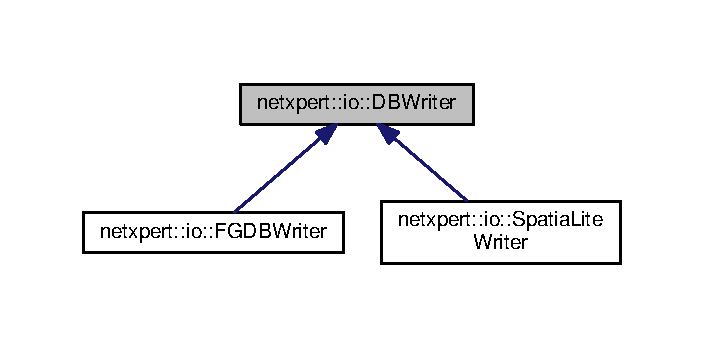
\includegraphics[width=338pt]{classnetxpert_1_1io_1_1DBWriter__inherit__graph}
\end{center}
\end{figure}
\subsection*{Public Member Functions}
\begin{DoxyCompactItemize}
\item 
virtual void {\bfseries Commit\+Current\+Transaction} ()=0\hypertarget{classnetxpert_1_1io_1_1DBWriter_aa6cbde221c9cb281fc564ec5947e4a89}{}\label{classnetxpert_1_1io_1_1DBWriter_aa6cbde221c9cb281fc564ec5947e4a89}

\item 
virtual void {\bfseries Create\+Net\+Xpert\+DB} ()=0\hypertarget{classnetxpert_1_1io_1_1DBWriter_a9aed2a197051fa97b389c9adf7bb5c3b}{}\label{classnetxpert_1_1io_1_1DBWriter_a9aed2a197051fa97b389c9adf7bb5c3b}

\item 
virtual void {\bfseries Create\+Solver\+Result\+Table} (const std\+::string \&\+\_\+table\+Name, const \hyperlink{namespacenetxpert_1_1data_a923ee7cb7eab8b9dbfd62fb6d26f51cb}{netxpert\+::data\+::\+Net\+Xpert\+Solver} solver\+Type)=0\hypertarget{classnetxpert_1_1io_1_1DBWriter_a605512371218841f9cfcfcd3d9badeb0}{}\label{classnetxpert_1_1io_1_1DBWriter_a605512371218841f9cfcfcd3d9badeb0}

\item 
virtual void {\bfseries Create\+Solver\+Result\+Table} (const std\+::string \&\+\_\+table\+Name, const \hyperlink{namespacenetxpert_1_1data_a923ee7cb7eab8b9dbfd62fb6d26f51cb}{netxpert\+::data\+::\+Net\+Xpert\+Solver} solver\+Type, const bool drop\+First)=0\hypertarget{classnetxpert_1_1io_1_1DBWriter_a35dd9c00f0621302fcf9e8fe4810e6ea}{}\label{classnetxpert_1_1io_1_1DBWriter_a35dd9c00f0621302fcf9e8fe4810e6ea}

\item 
virtual void {\bfseries Open\+New\+Transaction} ()=0\hypertarget{classnetxpert_1_1io_1_1DBWriter_a6c30c6e65624efc60019ca619b1a5822}{}\label{classnetxpert_1_1io_1_1DBWriter_a6c30c6e65624efc60019ca619b1a5822}

\item 
virtual void {\bfseries Close\+Connection} ()=0\hypertarget{classnetxpert_1_1io_1_1DBWriter_af660494aa22a5ef6106aed7c8262f336}{}\label{classnetxpert_1_1io_1_1DBWriter_af660494aa22a5ef6106aed7c8262f336}

\end{DoxyCompactItemize}


\subsection{Detailed Description}
Abstract \hyperlink{classClass}{Class} (Interface) for the output DB. 

The documentation for this class was generated from the following file\+:\begin{DoxyCompactItemize}
\item 
/home/hahne/dev/netxpert1\+\_\+0/include/dbwriter.\+h\end{DoxyCompactItemize}

\hypertarget{structnetxpert_1_1data_1_1DistributionArc}{}\section{netxpert\+:\+:data\+:\+:Distribution\+Arc Struct Reference}
\label{structnetxpert_1_1data_1_1DistributionArc}\index{netxpert\+::data\+::\+Distribution\+Arc@{netxpert\+::data\+::\+Distribution\+Arc}}


Data type for storing tuple $<$Compressed\+Path,flow$>$  




{\ttfamily \#include $<$data.\+h$>$}

\subsection*{Public Attributes}
\begin{DoxyCompactItemize}
\item 
\hyperlink{namespacenetxpert_1_1data_a82e488b55f222a9759d73e24f6087033}{Compressed\+Path} {\bfseries path}\hypertarget{structnetxpert_1_1data_1_1DistributionArc_ac7b77e587a4e3345afc59618db3e5b77}{}\label{structnetxpert_1_1data_1_1DistributionArc_ac7b77e587a4e3345afc59618db3e5b77}

\item 
flow\+\_\+t {\bfseries flow}\hypertarget{structnetxpert_1_1data_1_1DistributionArc_a43332bf5cc4f8341dda9d6c7b1eaeafb}{}\label{structnetxpert_1_1data_1_1DistributionArc_a43332bf5cc4f8341dda9d6c7b1eaeafb}

\end{DoxyCompactItemize}


\subsection{Detailed Description}
Data type for storing tuple $<$Compressed\+Path,flow$>$ 

The documentation for this struct was generated from the following file\+:\begin{DoxyCompactItemize}
\item 
/home/hahne/dev/netxpert1\+\_\+0/include/data.\+h\end{DoxyCompactItemize}

\hypertarget{structnetxpert_1_1data_1_1DuplicateArcData}{}\section{netxpert\+:\+:data\+:\+:Duplicate\+Arc\+Data Struct Reference}
\label{structnetxpert_1_1data_1_1DuplicateArcData}\index{netxpert\+::data\+::\+Duplicate\+Arc\+Data@{netxpert\+::data\+::\+Duplicate\+Arc\+Data}}


Data type for storing tuple $<$ext\+Arc\+ID,cost,capacity$>$  




{\ttfamily \#include $<$data.\+h$>$}

\subsection*{Public Attributes}
\begin{DoxyCompactItemize}
\item 
std\+::string {\bfseries ext\+Arc\+ID}\hypertarget{structnetxpert_1_1data_1_1DuplicateArcData_a389b60d12409b276c52e9fdcf3e3028a}{}\label{structnetxpert_1_1data_1_1DuplicateArcData_a389b60d12409b276c52e9fdcf3e3028a}

\item 
cost\+\_\+t {\bfseries cost}\hypertarget{structnetxpert_1_1data_1_1DuplicateArcData_afe676d824fbb93406e61d9f8461d205e}{}\label{structnetxpert_1_1data_1_1DuplicateArcData_afe676d824fbb93406e61d9f8461d205e}

\end{DoxyCompactItemize}


\subsection{Detailed Description}
Data type for storing tuple $<$ext\+Arc\+ID,cost,capacity$>$ 

The documentation for this struct was generated from the following file\+:\begin{DoxyCompactItemize}
\item 
/home/hahne/dev/netxpert1\+\_\+0/include/data.\+h\end{DoxyCompactItemize}

\hypertarget{classequal__to}{}\section{equal\+\_\+to Class Reference}
\label{classequal__to}\index{equal\+\_\+to@{equal\+\_\+to}}


\subsection{Detailed Description}
custom key type O\+D\+Pair in unordered map. 

The documentation for this class was generated from the following file\+:\begin{DoxyCompactItemize}
\item 
/home/hahne/dev/netxpert1\+\_\+0/include/data.\+h\end{DoxyCompactItemize}

\hypertarget{classequal__to}{}\section{equal\+\_\+to Class Reference}
\label{classequal__to}\index{equal\+\_\+to@{equal\+\_\+to}}


\subsection{Detailed Description}
custom key type O\+D\+Pair in unordered map. 

The documentation for this class was generated from the following file\+:\begin{DoxyCompactItemize}
\item 
/home/hahne/dev/netxpert1\+\_\+0/include/data.\+h\end{DoxyCompactItemize}

\hypertarget{classstd_1_1equal__to_3_01netxpert_1_1data_1_1InternalArc_01_4}{}\section{std\+:\+:equal\+\_\+to$<$ netxpert\+:\+:data\+:\+:Internal\+Arc $>$ Class Template Reference}
\label{classstd_1_1equal__to_3_01netxpert_1_1data_1_1InternalArc_01_4}\index{std\+::equal\+\_\+to$<$ netxpert\+::data\+::\+Internal\+Arc $>$@{std\+::equal\+\_\+to$<$ netxpert\+::data\+::\+Internal\+Arc $>$}}
\subsection*{Public Member Functions}
\begin{DoxyCompactItemize}
\item 
bool {\bfseries operator()} (const \hyperlink{structnetxpert_1_1data_1_1InternalArc}{netxpert\+::data\+::\+Internal\+Arc} \&a, const \hyperlink{structnetxpert_1_1data_1_1InternalArc}{netxpert\+::data\+::\+Internal\+Arc} \&b) const \hypertarget{classstd_1_1equal__to_3_01netxpert_1_1data_1_1InternalArc_01_4_a4b6538fb00825f540bc3e94d28027d38}{}\label{classstd_1_1equal__to_3_01netxpert_1_1data_1_1InternalArc_01_4_a4b6538fb00825f540bc3e94d28027d38}

\end{DoxyCompactItemize}


The documentation for this class was generated from the following file\+:\begin{DoxyCompactItemize}
\item 
/home/hahne/dev/netxpert1\+\_\+0/include/data.\+h\end{DoxyCompactItemize}

\hypertarget{structnetxpert_1_1data_1_1ExtClosestArcAndPoint}{}\section{netxpert\+:\+:data\+:\+:Ext\+Closest\+Arc\+And\+Point Struct Reference}
\label{structnetxpert_1_1data_1_1ExtClosestArcAndPoint}\index{netxpert\+::data\+::\+Ext\+Closest\+Arc\+And\+Point@{netxpert\+::data\+::\+Ext\+Closest\+Arc\+And\+Point}}
\subsection*{Public Attributes}
\begin{DoxyCompactItemize}
\item 
std\+::string {\bfseries ext\+Arc\+ID}\hypertarget{structnetxpert_1_1data_1_1ExtClosestArcAndPoint_a821aa8ee01fbd25c199e7f9fa770a44f}{}\label{structnetxpert_1_1data_1_1ExtClosestArcAndPoint_a821aa8ee01fbd25c199e7f9fa770a44f}

\item 
std\+::string {\bfseries ext\+From\+Node}\hypertarget{structnetxpert_1_1data_1_1ExtClosestArcAndPoint_abdaf7b5738f4ca5e710841d5ff7fd904}{}\label{structnetxpert_1_1data_1_1ExtClosestArcAndPoint_abdaf7b5738f4ca5e710841d5ff7fd904}

\item 
std\+::string {\bfseries ext\+To\+Node}\hypertarget{structnetxpert_1_1data_1_1ExtClosestArcAndPoint_aaf521441394e04cf1e18e91497c80691}{}\label{structnetxpert_1_1data_1_1ExtClosestArcAndPoint_aaf521441394e04cf1e18e91497c80691}

\item 
cost\+\_\+t {\bfseries cost}\hypertarget{structnetxpert_1_1data_1_1ExtClosestArcAndPoint_a0f5a880f5145e32f971512eaf9b5983b}{}\label{structnetxpert_1_1data_1_1ExtClosestArcAndPoint_a0f5a880f5145e32f971512eaf9b5983b}

\item 
capacity\+\_\+t {\bfseries capacity}\hypertarget{structnetxpert_1_1data_1_1ExtClosestArcAndPoint_a350fa54bc26af1bf561752df97cff106}{}\label{structnetxpert_1_1data_1_1ExtClosestArcAndPoint_a350fa54bc26af1bf561752df97cff106}

\item 
geos\+::geom\+::\+Coordinate {\bfseries closest\+Point}\hypertarget{structnetxpert_1_1data_1_1ExtClosestArcAndPoint_a9b5d95aa9e2194b622866d1c45316082}{}\label{structnetxpert_1_1data_1_1ExtClosestArcAndPoint_a9b5d95aa9e2194b622866d1c45316082}

\item 
std\+::shared\+\_\+ptr$<$ geos\+::geom\+::\+Geometry $>$ {\bfseries arc\+Geom}\hypertarget{structnetxpert_1_1data_1_1ExtClosestArcAndPoint_a294b37e5cb1c6e77380d163ecda306cd}{}\label{structnetxpert_1_1data_1_1ExtClosestArcAndPoint_a294b37e5cb1c6e77380d163ecda306cd}

\end{DoxyCompactItemize}


The documentation for this struct was generated from the following file\+:\begin{DoxyCompactItemize}
\item 
/home/hahne/dev/netxpert1\+\_\+0/include/data.\+h\end{DoxyCompactItemize}

\hypertarget{structnetxpert_1_1data_1_1ExtDistributionArc}{}\section{netxpert\+:\+:data\+:\+:Ext\+Distribution\+Arc Struct Reference}
\label{structnetxpert_1_1data_1_1ExtDistributionArc}\index{netxpert\+::data\+::\+Ext\+Distribution\+Arc@{netxpert\+::data\+::\+Ext\+Distribution\+Arc}}


Data type for storing tuple $<$ext\+Arc\+ID,ext\+Arc,cost,flow$>$  




{\ttfamily \#include $<$data.\+h$>$}



Collaboration diagram for netxpert\+:\+:data\+:\+:Ext\+Distribution\+Arc\+:\nopagebreak
\begin{figure}[H]
\begin{center}
\leavevmode
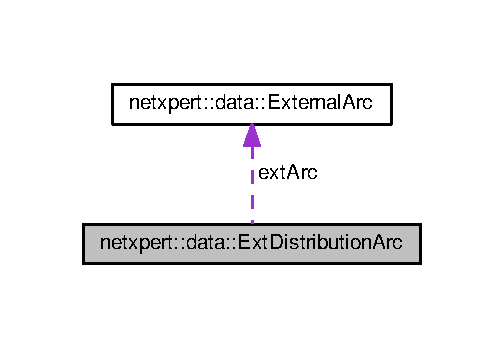
\includegraphics[width=242pt]{structnetxpert_1_1data_1_1ExtDistributionArc__coll__graph}
\end{center}
\end{figure}
\subsection*{Public Member Functions}
\begin{DoxyCompactItemize}
\item 
{\footnotesize template$<$class Archive $>$ }\\void {\bfseries serialize} (Archive \&ar)\hypertarget{structnetxpert_1_1data_1_1ExtDistributionArc_af3bf2382bfa90bafc9c80baa6e9e160b}{}\label{structnetxpert_1_1data_1_1ExtDistributionArc_af3bf2382bfa90bafc9c80baa6e9e160b}

\end{DoxyCompactItemize}
\subsection*{Public Attributes}
\begin{DoxyCompactItemize}
\item 
netxpert\+::data\+::\+Ext\+Arc\+ID {\bfseries arcid}\hypertarget{structnetxpert_1_1data_1_1ExtDistributionArc_a14b932c73adc34dd6cfb3cdbb39c6e95}{}\label{structnetxpert_1_1data_1_1ExtDistributionArc_a14b932c73adc34dd6cfb3cdbb39c6e95}

\item 
\hyperlink{structnetxpert_1_1data_1_1ExternalArc}{netxpert\+::data\+::\+External\+Arc} {\bfseries ext\+Arc}\hypertarget{structnetxpert_1_1data_1_1ExtDistributionArc_af4d9999cd6bbad0b55912f65911d0938}{}\label{structnetxpert_1_1data_1_1ExtDistributionArc_af4d9999cd6bbad0b55912f65911d0938}

\item 
cost\+\_\+t {\bfseries cost}\hypertarget{structnetxpert_1_1data_1_1ExtDistributionArc_a8c7c744b4dd482a8968299edaaa25cdf}{}\label{structnetxpert_1_1data_1_1ExtDistributionArc_a8c7c744b4dd482a8968299edaaa25cdf}

\item 
flow\+\_\+t {\bfseries flow}\hypertarget{structnetxpert_1_1data_1_1ExtDistributionArc_ad42ca648414668690de6b3c12dceba7b}{}\label{structnetxpert_1_1data_1_1ExtDistributionArc_ad42ca648414668690de6b3c12dceba7b}

\end{DoxyCompactItemize}


\subsection{Detailed Description}
Data type for storing tuple $<$ext\+Arc\+ID,ext\+Arc,cost,flow$>$ 

The documentation for this struct was generated from the following file\+:\begin{DoxyCompactItemize}
\item 
/home/hahne/dev/netxpert1\+\_\+0/include/data.\+h\end{DoxyCompactItemize}

\hypertarget{classExtension}{}\section{Extension Class Reference}
\label{classExtension}\index{Extension@{Extension}}


\subsection{Detailed Description}
key type O\+D\+Pair specifying how to hash; serves as key in unordered map. 

The documentation for this class was generated from the following file\+:\begin{DoxyCompactItemize}
\item 
/home/hahne/dev/netxpert1\+\_\+0/include/data.\+h\end{DoxyCompactItemize}

\hypertarget{classExtension}{}\section{Extension Class Reference}
\label{classExtension}\index{Extension@{Extension}}


\subsection{Detailed Description}
key type O\+D\+Pair specifying how to hash; serves as key in unordered map. 

The documentation for this class was generated from the following file\+:\begin{DoxyCompactItemize}
\item 
/home/hahne/dev/netxpert1\+\_\+0/include/data.\+h\end{DoxyCompactItemize}

\hypertarget{structnetxpert_1_1data_1_1ExternalArc}{}\section{netxpert\+:\+:data\+:\+:External\+Arc Struct Reference}
\label{structnetxpert_1_1data_1_1ExternalArc}\index{netxpert\+::data\+::\+External\+Arc@{netxpert\+::data\+::\+External\+Arc}}


Custom data type for storing external nodes tuple $<$from\+Node,to\+Node$>$ as simple type variant.  




{\ttfamily \#include $<$data.\+h$>$}

\subsection*{Public Member Functions}
\begin{DoxyCompactItemize}
\item 
{\footnotesize template$<$class Archive $>$ }\\void {\bfseries serialize} (Archive \&ar)\hypertarget{structnetxpert_1_1data_1_1ExternalArc_ac7c95273f4824d70da14c835ee8af62c}{}\label{structnetxpert_1_1data_1_1ExternalArc_ac7c95273f4824d70da14c835ee8af62c}

\end{DoxyCompactItemize}
\subsection*{Public Attributes}
\begin{DoxyCompactItemize}
\item 
std\+::string {\bfseries ext\+From\+Node}\hypertarget{structnetxpert_1_1data_1_1ExternalArc_ad151959688de67b567d6c6391f9182d4}{}\label{structnetxpert_1_1data_1_1ExternalArc_ad151959688de67b567d6c6391f9182d4}

\item 
std\+::string {\bfseries ext\+To\+Node}\hypertarget{structnetxpert_1_1data_1_1ExternalArc_a9f748154fb313753f42bafb658a47cdf}{}\label{structnetxpert_1_1data_1_1ExternalArc_a9f748154fb313753f42bafb658a47cdf}

\end{DoxyCompactItemize}


\subsection{Detailed Description}
Custom data type for storing external nodes tuple $<$from\+Node,to\+Node$>$ as simple type variant. 

The documentation for this struct was generated from the following file\+:\begin{DoxyCompactItemize}
\item 
/home/hahne/dev/netxpert1\+\_\+0/include/data.\+h\end{DoxyCompactItemize}

\hypertarget{structnetxpert_1_1data_1_1ExtNodeSupply}{}\section{netxpert\+:\+:data\+:\+:Ext\+Node\+Supply Struct Reference}
\label{structnetxpert_1_1data_1_1ExtNodeSupply}\index{netxpert\+::data\+::\+Ext\+Node\+Supply@{netxpert\+::data\+::\+Ext\+Node\+Supply}}


Data type for storing external node supply $<$ext\+Node\+ID,supply$>$ as simple type variant.  




{\ttfamily \#include $<$data.\+h$>$}

\subsection*{Public Member Functions}
\begin{DoxyCompactItemize}
\item 
{\footnotesize template$<$class Archive $>$ }\\void {\bfseries serialize} (Archive \&ar)\hypertarget{structnetxpert_1_1data_1_1ExtNodeSupply_a8cd30e2dd02383ac4530d68fe4c9d891}{}\label{structnetxpert_1_1data_1_1ExtNodeSupply_a8cd30e2dd02383ac4530d68fe4c9d891}

\end{DoxyCompactItemize}
\subsection*{Public Attributes}
\begin{DoxyCompactItemize}
\item 
netxpert\+::data\+::\+Ext\+Node\+ID {\bfseries ext\+Node\+ID}\hypertarget{structnetxpert_1_1data_1_1ExtNodeSupply_aaeff38c797587121ef750f7959995cd1}{}\label{structnetxpert_1_1data_1_1ExtNodeSupply_aaeff38c797587121ef750f7959995cd1}

\item 
supply\+\_\+t {\bfseries supply}\hypertarget{structnetxpert_1_1data_1_1ExtNodeSupply_a78243186ee0efdb852709054f2b21074}{}\label{structnetxpert_1_1data_1_1ExtNodeSupply_a78243186ee0efdb852709054f2b21074}

\end{DoxyCompactItemize}


\subsection{Detailed Description}
Data type for storing external node supply $<$ext\+Node\+ID,supply$>$ as simple type variant. 

The documentation for this struct was generated from the following file\+:\begin{DoxyCompactItemize}
\item 
/home/hahne/dev/netxpert1\+\_\+0/include/data.\+h\end{DoxyCompactItemize}

\hypertarget{structnetxpert_1_1data_1_1ExtODPair}{}\section{netxpert\+:\+:data\+:\+:Ext\+O\+D\+Pair Struct Reference}
\label{structnetxpert_1_1data_1_1ExtODPair}\index{netxpert\+::data\+::\+Ext\+O\+D\+Pair@{netxpert\+::data\+::\+Ext\+O\+D\+Pair}}


Custom data type for storing \hyperlink{structnetxpert_1_1data_1_1ExtODPair}{Ext\+O\+D\+Pair} tuple $<$origin,dest$>$ as simple type variant.  




{\ttfamily \#include $<$data.\+h$>$}

\subsection*{Public Member Functions}
\begin{DoxyCompactItemize}
\item 
bool {\bfseries operator==} (const \hyperlink{structnetxpert_1_1data_1_1ExtODPair}{Ext\+O\+D\+Pair} \&p2) const \hypertarget{structnetxpert_1_1data_1_1ExtODPair_a8209b9b7fe51bf55a73ca4fde3120627}{}\label{structnetxpert_1_1data_1_1ExtODPair_a8209b9b7fe51bf55a73ca4fde3120627}

\item 
{\footnotesize template$<$class Archive $>$ }\\void {\bfseries serialize} (Archive \&ar)\hypertarget{structnetxpert_1_1data_1_1ExtODPair_aed8b2cd85d2ddcb2e3c76512e8eeae21}{}\label{structnetxpert_1_1data_1_1ExtODPair_aed8b2cd85d2ddcb2e3c76512e8eeae21}

\end{DoxyCompactItemize}
\subsection*{Public Attributes}
\begin{DoxyCompactItemize}
\item 
uint32\+\_\+t {\bfseries origin}\hypertarget{structnetxpert_1_1data_1_1ExtODPair_a35f843db5fc7705ab12959727bc528b4}{}\label{structnetxpert_1_1data_1_1ExtODPair_a35f843db5fc7705ab12959727bc528b4}

\item 
uint32\+\_\+t {\bfseries dest}\hypertarget{structnetxpert_1_1data_1_1ExtODPair_ae38c7608bba39a2d32ef1a5ea6e4c187}{}\label{structnetxpert_1_1data_1_1ExtODPair_ae38c7608bba39a2d32ef1a5ea6e4c187}

\end{DoxyCompactItemize}


\subsection{Detailed Description}
Custom data type for storing \hyperlink{structnetxpert_1_1data_1_1ExtODPair}{Ext\+O\+D\+Pair} tuple $<$origin,dest$>$ as simple type variant. 

The documentation for this struct was generated from the following file\+:\begin{DoxyCompactItemize}
\item 
/home/hahne/dev/netxpert1\+\_\+0/include/data.\+h\end{DoxyCompactItemize}

\hypertarget{structnetxpert_1_1data_1_1ExtSPTreeArc}{}\section{netxpert\+:\+:data\+:\+:Ext\+S\+P\+Tree\+Arc Struct Reference}
\label{structnetxpert_1_1data_1_1ExtSPTreeArc}\index{netxpert\+::data\+::\+Ext\+S\+P\+Tree\+Arc@{netxpert\+::data\+::\+Ext\+S\+P\+Tree\+Arc}}


Custom data type for storing external arc of S\+P\+Tree/\+O\+D\+Matrix $<$ext\+From\+Node,ext\+To\+Node,cost$>$ as simple type variant.  




{\ttfamily \#include $<$data.\+h$>$}



Collaboration diagram for netxpert\+:\+:data\+:\+:Ext\+S\+P\+Tree\+Arc\+:\nopagebreak
\begin{figure}[H]
\begin{center}
\leavevmode
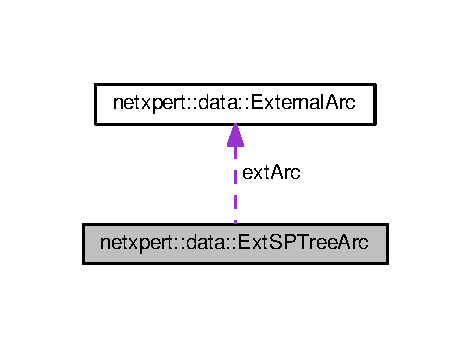
\includegraphics[width=226pt]{structnetxpert_1_1data_1_1ExtSPTreeArc__coll__graph}
\end{center}
\end{figure}
\subsection*{Public Member Functions}
\begin{DoxyCompactItemize}
\item 
{\footnotesize template$<$class Archive $>$ }\\void {\bfseries serialize} (Archive \&ar)\hypertarget{structnetxpert_1_1data_1_1ExtSPTreeArc_a56e7f1d95674c14d505d897e2a34506b}{}\label{structnetxpert_1_1data_1_1ExtSPTreeArc_a56e7f1d95674c14d505d897e2a34506b}

\end{DoxyCompactItemize}
\subsection*{Public Attributes}
\begin{DoxyCompactItemize}
\item 
netxpert\+::data\+::\+Ext\+Arc\+ID {\bfseries ext\+Arc\+ID}\hypertarget{structnetxpert_1_1data_1_1ExtSPTreeArc_ab5d23ea88dab7a425dc6c9f7135f0f56}{}\label{structnetxpert_1_1data_1_1ExtSPTreeArc_ab5d23ea88dab7a425dc6c9f7135f0f56}

\item 
\hyperlink{structnetxpert_1_1data_1_1ExternalArc}{netxpert\+::data\+::\+External\+Arc} {\bfseries ext\+Arc}\hypertarget{structnetxpert_1_1data_1_1ExtSPTreeArc_ab867b9d9f89891afd0b789f806b94b60}{}\label{structnetxpert_1_1data_1_1ExtSPTreeArc_ab867b9d9f89891afd0b789f806b94b60}

\item 
cost\+\_\+t {\bfseries cost}\hypertarget{structnetxpert_1_1data_1_1ExtSPTreeArc_a9c473340c0d1071a14eed68f5750f37f}{}\label{structnetxpert_1_1data_1_1ExtSPTreeArc_a9c473340c0d1071a14eed68f5750f37f}

\end{DoxyCompactItemize}


\subsection{Detailed Description}
Custom data type for storing external arc of S\+P\+Tree/\+O\+D\+Matrix $<$ext\+From\+Node,ext\+To\+Node,cost$>$ as simple type variant. 

The documentation for this struct was generated from the following file\+:\begin{DoxyCompactItemize}
\item 
/home/hahne/dev/netxpert1\+\_\+0/include/data.\+h\end{DoxyCompactItemize}

\hypertarget{structnetxpert_1_1data_1_1ExtTransportationData}{}\section{netxpert\+:\+:data\+:\+:Ext\+Transportation\+Data Struct Reference}
\label{structnetxpert_1_1data_1_1ExtTransportationData}\index{netxpert\+::data\+::\+Ext\+Transportation\+Data@{netxpert\+::data\+::\+Ext\+Transportation\+Data}}
\subsection*{Public Member Functions}
\begin{DoxyCompactItemize}
\item 
{\footnotesize template$<$class Archive $>$ }\\void {\bfseries serialize} (Archive \&ar)\hypertarget{structnetxpert_1_1data_1_1ExtTransportationData_a89f3a53b514bb3a1b5859e3561ac295f}{}\label{structnetxpert_1_1data_1_1ExtTransportationData_a89f3a53b514bb3a1b5859e3561ac295f}

\end{DoxyCompactItemize}
\subsection*{Public Attributes}
\begin{DoxyCompactItemize}
\item 
netxpert\+::data\+::\+Ext\+S\+P\+T\+Arcs {\bfseries odm}\hypertarget{structnetxpert_1_1data_1_1ExtTransportationData_a0d58e4a34c31679a87e411a5059a22f4}{}\label{structnetxpert_1_1data_1_1ExtTransportationData_a0d58e4a34c31679a87e411a5059a22f4}

\item 
netxpert\+::data\+::\+Ext\+Node\+Supplies {\bfseries supply}\hypertarget{structnetxpert_1_1data_1_1ExtTransportationData_a60dc77c5bf8dc0e33c7eb447c6cf7e08}{}\label{structnetxpert_1_1data_1_1ExtTransportationData_a60dc77c5bf8dc0e33c7eb447c6cf7e08}

\end{DoxyCompactItemize}


The documentation for this struct was generated from the following file\+:\begin{DoxyCompactItemize}
\item 
/home/hahne/dev/netxpert1\+\_\+0/include/data.\+h\end{DoxyCompactItemize}

\hypertarget{classnetxpert_1_1io_1_1FGDBWriter}{}\section{netxpert\+:\+:io\+:\+:F\+G\+D\+B\+Writer Class Reference}
\label{classnetxpert_1_1io_1_1FGDBWriter}\index{netxpert\+::io\+::\+F\+G\+D\+B\+Writer@{netxpert\+::io\+::\+F\+G\+D\+B\+Writer}}


Writes the result of Net\+Xpert into a E\+S\+RI File\+Geodatabase.  




{\ttfamily \#include $<$fgdbwriter.\+h$>$}



Inheritance diagram for netxpert\+:\+:io\+:\+:F\+G\+D\+B\+Writer\+:\nopagebreak
\begin{figure}[H]
\begin{center}
\leavevmode
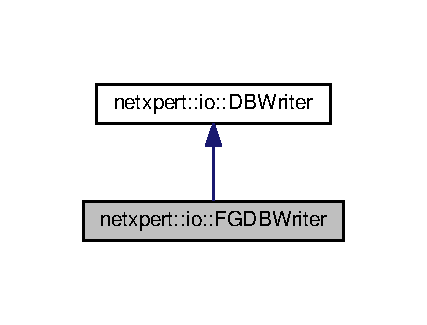
\includegraphics[width=205pt]{classnetxpert_1_1io_1_1FGDBWriter__inherit__graph}
\end{center}
\end{figure}


Collaboration diagram for netxpert\+:\+:io\+:\+:F\+G\+D\+B\+Writer\+:\nopagebreak
\begin{figure}[H]
\begin{center}
\leavevmode
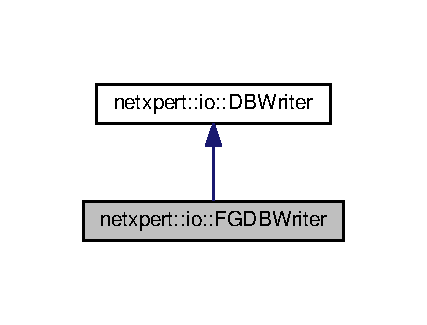
\includegraphics[width=205pt]{classnetxpert_1_1io_1_1FGDBWriter__coll__graph}
\end{center}
\end{figure}
\subsection*{Public Member Functions}
\begin{DoxyCompactItemize}
\item 
{\bfseries F\+G\+D\+B\+Writer} (\hyperlink{structnetxpert_1_1cnfg_1_1Config}{netxpert\+::cnfg\+::\+Config} \&netxpert\+Config)\hypertarget{classnetxpert_1_1io_1_1FGDBWriter_aa61e7d22c7bf7c12400c830a712ff5ab}{}\label{classnetxpert_1_1io_1_1FGDBWriter_aa61e7d22c7bf7c12400c830a712ff5ab}

\item 
void {\bfseries Commit\+Current\+Transaction} ()\hypertarget{classnetxpert_1_1io_1_1FGDBWriter_a18e8afe6996ff6cc492cd41134998068}{}\label{classnetxpert_1_1io_1_1FGDBWriter_a18e8afe6996ff6cc492cd41134998068}

\item 
void {\bfseries Create\+Net\+Xpert\+DB} ()\hypertarget{classnetxpert_1_1io_1_1FGDBWriter_ae99c6ad785d867ae2978f447ce96a2b6}{}\label{classnetxpert_1_1io_1_1FGDBWriter_ae99c6ad785d867ae2978f447ce96a2b6}

\item 
void {\bfseries Create\+Solver\+Result\+Table} (const std\+::string \&\+\_\+table\+Name, const \hyperlink{namespacenetxpert_1_1data_a923ee7cb7eab8b9dbfd62fb6d26f51cb}{netxpert\+::data\+::\+Net\+Xpert\+Solver} solver\+Type)\hypertarget{classnetxpert_1_1io_1_1FGDBWriter_a76e57985a136af8618f36e480525b3d2}{}\label{classnetxpert_1_1io_1_1FGDBWriter_a76e57985a136af8618f36e480525b3d2}

\item 
void {\bfseries Create\+Solver\+Result\+Table} (const std\+::string \&\+\_\+table\+Name, const \hyperlink{namespacenetxpert_1_1data_a923ee7cb7eab8b9dbfd62fb6d26f51cb}{netxpert\+::data\+::\+Net\+Xpert\+Solver} solver\+Type, const bool drop\+First)\hypertarget{classnetxpert_1_1io_1_1FGDBWriter_a640ffa09d53425d1823fd98a5faaaa90}{}\label{classnetxpert_1_1io_1_1FGDBWriter_a640ffa09d53425d1823fd98a5faaaa90}

\item 
void {\bfseries Open\+New\+Transaction} ()\hypertarget{classnetxpert_1_1io_1_1FGDBWriter_a71bd85819e7a1ca4097cc845b03f3806}{}\label{classnetxpert_1_1io_1_1FGDBWriter_a71bd85819e7a1ca4097cc845b03f3806}

\item 
void \hyperlink{classnetxpert_1_1io_1_1FGDBWriter_a10935bb3b8a9b96ca5982020133c6da2}{Save\+Network\+Builder\+Arc} (const std\+::string \&ext\+Arc\+ID, const uint32\+\_\+t from\+Node, const uint32\+\_\+t to\+Node, const double cost, const double capacity, const std\+::string \&oneway, const geos\+::geom\+::\+Geometry \&arc, const std\+::string \&\+\_\+table\+Name)
\item 
void {\bfseries Save\+Result\+Arc} (const std\+::string \&orig, const std\+::string \&dest, const double cost, const double capacity, const double flow, const geos\+::geom\+::\+Multi\+Line\+String \&route, const std\+::string \&\+\_\+table\+Name)\hypertarget{classnetxpert_1_1io_1_1FGDBWriter_a2ce305e5b6be31fbb4915f23589d3f58}{}\label{classnetxpert_1_1io_1_1FGDBWriter_a2ce305e5b6be31fbb4915f23589d3f58}

\item 
void {\bfseries Save\+Result\+Arc} (const std\+::string \&orig, const std\+::string \&dest, const double cost, const geos\+::geom\+::\+Multi\+Line\+String \&route, const std\+::string \&\+\_\+table\+Name)\hypertarget{classnetxpert_1_1io_1_1FGDBWriter_a20881849b5ae7818364f1b62dd41f983}{}\label{classnetxpert_1_1io_1_1FGDBWriter_a20881849b5ae7818364f1b62dd41f983}

\item 
void {\bfseries Save\+Result\+Arc} (const std\+::string \&original\+Arc\+ID, const double cost, const geos\+::geom\+::\+Multi\+Line\+String \&route, const std\+::string \&\+\_\+table\+Name)\hypertarget{classnetxpert_1_1io_1_1FGDBWriter_a0446693ad1ab99dce0471a575bf04a66}{}\label{classnetxpert_1_1io_1_1FGDBWriter_a0446693ad1ab99dce0471a575bf04a66}

\item 
void {\bfseries Save\+Result\+Arc} (const std\+::string \&orig, const double cost, const double cutoff, const geos\+::geom\+::\+Multi\+Line\+String \&route, const std\+::string \&\+\_\+table\+Name)\hypertarget{classnetxpert_1_1io_1_1FGDBWriter_a2ed233090b6e8feb2eff6207dbea7d0a}{}\label{classnetxpert_1_1io_1_1FGDBWriter_a2ed233090b6e8feb2eff6207dbea7d0a}

\item 
void {\bfseries Close\+Connection} ()\hypertarget{classnetxpert_1_1io_1_1FGDBWriter_af86818c4b41f226846754a3746ec009d}{}\label{classnetxpert_1_1io_1_1FGDBWriter_af86818c4b41f226846754a3746ec009d}

\end{DoxyCompactItemize}


\subsection{Detailed Description}
Writes the result of Net\+Xpert into a E\+S\+RI File\+Geodatabase. 

\subsection{Member Function Documentation}
\index{netxpert\+::io\+::\+F\+G\+D\+B\+Writer@{netxpert\+::io\+::\+F\+G\+D\+B\+Writer}!Save\+Network\+Builder\+Arc@{Save\+Network\+Builder\+Arc}}
\index{Save\+Network\+Builder\+Arc@{Save\+Network\+Builder\+Arc}!netxpert\+::io\+::\+F\+G\+D\+B\+Writer@{netxpert\+::io\+::\+F\+G\+D\+B\+Writer}}
\subsubsection[{\texorpdfstring{Save\+Network\+Builder\+Arc(const std\+::string \&ext\+Arc\+I\+D, const uint32\+\_\+t from\+Node, const uint32\+\_\+t to\+Node, const double cost, const double capacity, const std\+::string \&oneway, const geos\+::geom\+::\+Geometry \&arc, const std\+::string \&\+\_\+table\+Name)}{SaveNetworkBuilderArc(const std::string &extArcID, const uint32_t fromNode, const uint32_t toNode, const double cost, const double capacity, const std::string &oneway, const geos::geom::Geometry &arc, const std::string &_tableName)}}]{\setlength{\rightskip}{0pt plus 5cm}void netxpert\+::io\+::\+F\+G\+D\+B\+Writer\+::\+Save\+Network\+Builder\+Arc (
\begin{DoxyParamCaption}
\item[{const std\+::string \&}]{ext\+Arc\+ID, }
\item[{const uint32\+\_\+t}]{from\+Node, }
\item[{const uint32\+\_\+t}]{to\+Node, }
\item[{const double}]{cost, }
\item[{const double}]{capacity, }
\item[{const std\+::string \&}]{oneway, }
\item[{const geos\+::geom\+::\+Geometry \&}]{arc, }
\item[{const std\+::string \&}]{\+\_\+table\+Name}
\end{DoxyParamCaption}
)}\hypertarget{classnetxpert_1_1io_1_1FGDBWriter_a10935bb3b8a9b96ca5982020133c6da2}{}\label{classnetxpert_1_1io_1_1FGDBWriter_a10935bb3b8a9b96ca5982020133c6da2}
For saving the result arc of a built network into the net\+Xpert result DB 

The documentation for this class was generated from the following file\+:\begin{DoxyCompactItemize}
\item 
/home/hahne/dev/netxpert1\+\_\+0/include/fgdbwriter.\+h\end{DoxyCompactItemize}

\hypertarget{structnetxpert_1_1data_1_1FlowCost}{}\section{netxpert\+:\+:data\+:\+:Flow\+Cost Struct Reference}
\label{structnetxpert_1_1data_1_1FlowCost}\index{netxpert\+::data\+::\+Flow\+Cost@{netxpert\+::data\+::\+Flow\+Cost}}


Data type for storing tuple $<$from\+Node,to\+Node,flow,cost$>$  




{\ttfamily \#include $<$data.\+h$>$}

\subsection*{Public Attributes}
\begin{DoxyCompactItemize}
\item 
arc\+\_\+t {\bfseries int\+Arc}\hypertarget{structnetxpert_1_1data_1_1FlowCost_a51a06cd2018eebbb38eccc2de816c7aa}{}\label{structnetxpert_1_1data_1_1FlowCost_a51a06cd2018eebbb38eccc2de816c7aa}

\item 
capacity\+\_\+t {\bfseries flow}\hypertarget{structnetxpert_1_1data_1_1FlowCost_ad162527ddd7887b64b1cd2c1a3c5194c}{}\label{structnetxpert_1_1data_1_1FlowCost_ad162527ddd7887b64b1cd2c1a3c5194c}

\item 
cost\+\_\+t {\bfseries cost}\hypertarget{structnetxpert_1_1data_1_1FlowCost_a098fccc5cac184b83536f1490efd5716}{}\label{structnetxpert_1_1data_1_1FlowCost_a098fccc5cac184b83536f1490efd5716}

\end{DoxyCompactItemize}


\subsection{Detailed Description}
Data type for storing tuple $<$from\+Node,to\+Node,flow,cost$>$ 

The documentation for this struct was generated from the following file\+:\begin{DoxyCompactItemize}
\item 
/home/hahne/dev/netxpert1\+\_\+0/include/data.\+h\end{DoxyCompactItemize}

\hypertarget{classstd_1_1hash_3_01netxpert_1_1data_1_1InternalArc_01_4}{}\section{std\+:\+:hash$<$ netxpert\+:\+:data\+:\+:Internal\+Arc $>$ Class Template Reference}
\label{classstd_1_1hash_3_01netxpert_1_1data_1_1InternalArc_01_4}\index{std\+::hash$<$ netxpert\+::data\+::\+Internal\+Arc $>$@{std\+::hash$<$ netxpert\+::data\+::\+Internal\+Arc $>$}}
\subsection*{Public Member Functions}
\begin{DoxyCompactItemize}
\item 
long {\bfseries operator()} (const \hyperlink{structnetxpert_1_1data_1_1InternalArc}{netxpert\+::data\+::\+Internal\+Arc} \&x) const \hypertarget{classstd_1_1hash_3_01netxpert_1_1data_1_1InternalArc_01_4_a789af0a23bd7d548a7ab16850cb9ad6c}{}\label{classstd_1_1hash_3_01netxpert_1_1data_1_1InternalArc_01_4_a789af0a23bd7d548a7ab16850cb9ad6c}

\end{DoxyCompactItemize}


The documentation for this class was generated from the following file\+:\begin{DoxyCompactItemize}
\item 
/home/hahne/dev/netxpert1\+\_\+0/include/data.\+h\end{DoxyCompactItemize}

\hypertarget{classnetxpert_1_1core_1_1IMinCostFlow}{}\section{netxpert\+:\+:core\+:\+:I\+Min\+Cost\+Flow Class Reference}
\label{classnetxpert_1_1core_1_1IMinCostFlow}\index{netxpert\+::core\+::\+I\+Min\+Cost\+Flow@{netxpert\+::core\+::\+I\+Min\+Cost\+Flow}}


Abstract \hyperlink{classClass}{Class} (Interface) for all Minimum Cost Flow Problem Solvers in netxpert core.  




{\ttfamily \#include $<$imcflow.\+h$>$}



Inheritance diagram for netxpert\+:\+:core\+:\+:I\+Min\+Cost\+Flow\+:\nopagebreak
\begin{figure}[H]
\begin{center}
\leavevmode
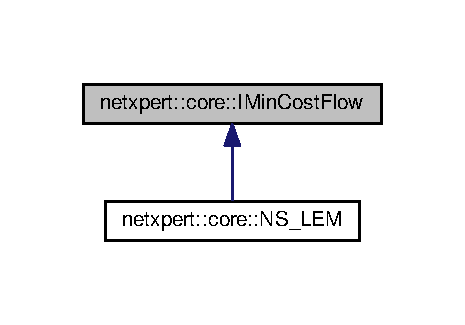
\includegraphics[width=223pt]{classnetxpert_1_1core_1_1IMinCostFlow__inherit__graph}
\end{center}
\end{figure}
\subsection*{Public Member Functions}
\begin{DoxyCompactItemize}
\item 
virtual void {\bfseries Load\+Net} (const uint32\+\_\+t nmax, const uint32\+\_\+t mmax, lemon\+::\+Filter\+Arcs$<$ netxpert\+::data\+::graph\+\_\+t, netxpert\+::data\+::graph\+\_\+t\+::\+Arc\+Map$<$ bool $>$$>$ $\ast$sg, netxpert\+::data\+::graph\+\_\+t\+::\+Arc\+Map$<$ netxpert\+::data\+::cost\+\_\+t $>$ $\ast$\+\_\+cost\+Map, netxpert\+::data\+::graph\+\_\+t\+::\+Arc\+Map$<$ netxpert\+::data\+::capacity\+\_\+t $>$ $\ast$\+\_\+cap\+Map, netxpert\+::data\+::graph\+\_\+t\+::\+Node\+Map$<$ netxpert\+::data\+::supply\+\_\+t $>$ $\ast$\+\_\+supply\+Map)=0\hypertarget{classnetxpert_1_1core_1_1IMinCostFlow_afe4ac0e1320c36cbccbb6c97e0c05765}{}\label{classnetxpert_1_1core_1_1IMinCostFlow_afe4ac0e1320c36cbccbb6c97e0c05765}

\item 
virtual const uint32\+\_\+t {\bfseries Get\+Arc\+Count} ()=0\hypertarget{classnetxpert_1_1core_1_1IMinCostFlow_afc43c05d492c96e3795c844636ff3a6a}{}\label{classnetxpert_1_1core_1_1IMinCostFlow_afc43c05d492c96e3795c844636ff3a6a}

\item 
virtual const uint32\+\_\+t {\bfseries Get\+Node\+Count} ()=0\hypertarget{classnetxpert_1_1core_1_1IMinCostFlow_a0d09f6b1be2a843c3dd8da0377cd43ba}{}\label{classnetxpert_1_1core_1_1IMinCostFlow_a0d09f6b1be2a843c3dd8da0377cd43ba}

\item 
virtual void {\bfseries Solve\+M\+CF} ()=0\hypertarget{classnetxpert_1_1core_1_1IMinCostFlow_a4730faf5a646cb01130a3dd36e3205ba}{}\label{classnetxpert_1_1core_1_1IMinCostFlow_a4730faf5a646cb01130a3dd36e3205ba}

\item 
virtual const double {\bfseries Get\+Optimum} () const =0\hypertarget{classnetxpert_1_1core_1_1IMinCostFlow_a2828271d5ac69c015f431cd5793ab661}{}\label{classnetxpert_1_1core_1_1IMinCostFlow_a2828271d5ac69c015f431cd5793ab661}

\item 
virtual std\+::vector$<$ netxpert\+::data\+::arc\+\_\+t $>$ {\bfseries Get\+M\+C\+F\+Arcs} ()=0\hypertarget{classnetxpert_1_1core_1_1IMinCostFlow_a664df6422560419a23e49c5948e4ace4}{}\label{classnetxpert_1_1core_1_1IMinCostFlow_a664df6422560419a23e49c5948e4ace4}

\item 
virtual netxpert\+::data\+::graph\+\_\+t\+::\+Arc\+Map$<$ netxpert\+::data\+::flow\+\_\+t $>$ $\ast$ {\bfseries Get\+M\+C\+F\+Flow} ()=0\hypertarget{classnetxpert_1_1core_1_1IMinCostFlow_ac1303e3c31a2f4e2ec11e6ddc1ee0a30}{}\label{classnetxpert_1_1core_1_1IMinCostFlow_ac1303e3c31a2f4e2ec11e6ddc1ee0a30}

\item 
virtual netxpert\+::data\+::graph\+\_\+t\+::\+Arc\+Map$<$ netxpert\+::data\+::cost\+\_\+t $>$ $\ast$ {\bfseries Get\+M\+C\+F\+Cost} ()=0\hypertarget{classnetxpert_1_1core_1_1IMinCostFlow_a1262b923b11fc3b240c2e61f1e2e7f07}{}\label{classnetxpert_1_1core_1_1IMinCostFlow_a1262b923b11fc3b240c2e61f1e2e7f07}

\item 
virtual const int {\bfseries Get\+M\+C\+F\+Status} ()=0\hypertarget{classnetxpert_1_1core_1_1IMinCostFlow_a71466b0a2c494afb015197a103ec0dcc}{}\label{classnetxpert_1_1core_1_1IMinCostFlow_a71466b0a2c494afb015197a103ec0dcc}

\end{DoxyCompactItemize}


\subsection{Detailed Description}
Abstract \hyperlink{classClass}{Class} (Interface) for all Minimum Cost Flow Problem Solvers in netxpert core. 

The documentation for this class was generated from the following file\+:\begin{DoxyCompactItemize}
\item 
/home/hahne/dev/netxpert1\+\_\+0/include/core/imcflow.\+h\end{DoxyCompactItemize}

\hypertarget{classnetxpert_1_1core_1_1IMinSpanTree}{}\section{netxpert\+:\+:core\+:\+:I\+Min\+Span\+Tree Class Reference}
\label{classnetxpert_1_1core_1_1IMinSpanTree}\index{netxpert\+::core\+::\+I\+Min\+Span\+Tree@{netxpert\+::core\+::\+I\+Min\+Span\+Tree}}


Abstract \hyperlink{classClass}{Class} (Interface) for all Minimum Spanning Tree Solvers in netxpert core.  




{\ttfamily \#include $<$imstree.\+h$>$}



Inheritance diagram for netxpert\+:\+:core\+:\+:I\+Min\+Span\+Tree\+:\nopagebreak
\begin{figure}[H]
\begin{center}
\leavevmode
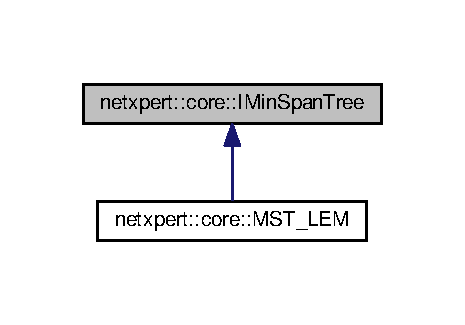
\includegraphics[width=223pt]{classnetxpert_1_1core_1_1IMinSpanTree__inherit__graph}
\end{center}
\end{figure}
\subsection*{Public Member Functions}
\begin{DoxyCompactItemize}
\item 
virtual \hyperlink{classnetxpert_1_1core_1_1IMinSpanTree_a6179745c4e3b91c1cc4260ff43a40a07}{$\sim$\+I\+Min\+Span\+Tree} ()
\item 
virtual void {\bfseries Load\+Net} (const uint32\+\_\+t nmax, const uint32\+\_\+t mmax, lemon\+::\+Filter\+Arcs$<$ netxpert\+::data\+::graph\+\_\+t, netxpert\+::data\+::graph\+\_\+t\+::\+Arc\+Map$<$ bool $>$$>$ $\ast$sg, netxpert\+::data\+::graph\+\_\+t\+::\+Arc\+Map$<$ netxpert\+::data\+::cost\+\_\+t $>$ $\ast$cm)=0\hypertarget{classnetxpert_1_1core_1_1IMinSpanTree_afe3b59f776882e4b645fb53f2000a363}{}\label{classnetxpert_1_1core_1_1IMinSpanTree_afe3b59f776882e4b645fb53f2000a363}

\item 
virtual const uint32\+\_\+t {\bfseries Get\+Arc\+Count} ()=0\hypertarget{classnetxpert_1_1core_1_1IMinSpanTree_ae4b36350ca156e0d1f507c6c6acb1e71}{}\label{classnetxpert_1_1core_1_1IMinSpanTree_ae4b36350ca156e0d1f507c6c6acb1e71}

\item 
virtual const uint32\+\_\+t {\bfseries Get\+Node\+Count} ()=0\hypertarget{classnetxpert_1_1core_1_1IMinSpanTree_aaf79eb23e96a7dc1030c88298a800f98}{}\label{classnetxpert_1_1core_1_1IMinSpanTree_aaf79eb23e96a7dc1030c88298a800f98}

\item 
virtual void {\bfseries Solve\+M\+ST} ()=0\hypertarget{classnetxpert_1_1core_1_1IMinSpanTree_af1f5ddfaed28ad881c376746fd448e58}{}\label{classnetxpert_1_1core_1_1IMinSpanTree_af1f5ddfaed28ad881c376746fd448e58}

\item 
virtual const double {\bfseries Get\+Optimum} () const =0\hypertarget{classnetxpert_1_1core_1_1IMinSpanTree_a3c5b7486449a768eccb92ac1bc7ee446}{}\label{classnetxpert_1_1core_1_1IMinSpanTree_a3c5b7486449a768eccb92ac1bc7ee446}

\item 
virtual std\+::vector$<$ netxpert\+::data\+::arc\+\_\+t $>$ {\bfseries Get\+M\+ST} ()=0\hypertarget{classnetxpert_1_1core_1_1IMinSpanTree_a0c31d5383b3a26be340db74d543c8d88}{}\label{classnetxpert_1_1core_1_1IMinSpanTree_a0c31d5383b3a26be340db74d543c8d88}

\end{DoxyCompactItemize}


\subsection{Detailed Description}
Abstract \hyperlink{classClass}{Class} (Interface) for all Minimum Spanning Tree Solvers in netxpert core. 

\subsection{Constructor \& Destructor Documentation}
\index{netxpert\+::core\+::\+I\+Min\+Span\+Tree@{netxpert\+::core\+::\+I\+Min\+Span\+Tree}!````~I\+Min\+Span\+Tree@{$\sim$\+I\+Min\+Span\+Tree}}
\index{````~I\+Min\+Span\+Tree@{$\sim$\+I\+Min\+Span\+Tree}!netxpert\+::core\+::\+I\+Min\+Span\+Tree@{netxpert\+::core\+::\+I\+Min\+Span\+Tree}}
\subsubsection[{\texorpdfstring{$\sim$\+I\+Min\+Span\+Tree()}{~IMinSpanTree()}}]{\setlength{\rightskip}{0pt plus 5cm}virtual netxpert\+::core\+::\+I\+Min\+Span\+Tree\+::$\sim$\+I\+Min\+Span\+Tree (
\begin{DoxyParamCaption}
{}
\end{DoxyParamCaption}
)\hspace{0.3cm}{\ttfamily [inline]}, {\ttfamily [virtual]}}\hypertarget{classnetxpert_1_1core_1_1IMinSpanTree_a6179745c4e3b91c1cc4260ff43a40a07}{}\label{classnetxpert_1_1core_1_1IMinSpanTree_a6179745c4e3b91c1cc4260ff43a40a07}
Default destructor 

The documentation for this class was generated from the following file\+:\begin{DoxyCompactItemize}
\item 
/home/hahne/dev/netxpert1\+\_\+0/include/core/imstree.\+h\end{DoxyCompactItemize}

\hypertarget{classnetxpert_1_1core_1_1Inf}{}\section{netxpert\+:\+:core\+:\+:Inf$<$ T $>$ Class Template Reference}
\label{classnetxpert_1_1core_1_1Inf}\index{netxpert\+::core\+::\+Inf$<$ T $>$@{netxpert\+::core\+::\+Inf$<$ T $>$}}


Modeling Infinity for the given type T.  




{\ttfamily \#include $<$sptlem.\+h$>$}

\subsection*{Public Member Functions}
\begin{DoxyCompactItemize}
\item 
{\bfseries operator T} ()\hypertarget{classnetxpert_1_1core_1_1Inf_a850daa0b653488313b63afe256aa0c58}{}\label{classnetxpert_1_1core_1_1Inf_a850daa0b653488313b63afe256aa0c58}

\end{DoxyCompactItemize}


\subsection{Detailed Description}
\subsubsection*{template$<$typename T$>$\\*
class netxpert\+::core\+::\+Inf$<$ T $>$}

Modeling Infinity for the given type T. 

The documentation for this class was generated from the following file\+:\begin{DoxyCompactItemize}
\item 
/home/hahne/dev/netxpert1\+\_\+0/include/core/sptlem.\+h\end{DoxyCompactItemize}

\hypertarget{structnetxpert_1_1data_1_1InputArc}{}\section{netxpert\+:\+:data\+:\+:Input\+Arc Struct Reference}
\label{structnetxpert_1_1data_1_1InputArc}\index{netxpert\+::data\+::\+Input\+Arc@{netxpert\+::data\+::\+Input\+Arc}}


Data type for storing tuple $<$ext\+Arc\+ID,ext\+From\+Node,ext\+To\+Node,cost,capacity,oneway$>$  




{\ttfamily \#include $<$data.\+h$>$}

\subsection*{Public Attributes}
\begin{DoxyCompactItemize}
\item 
std\+::string {\bfseries ext\+Arc\+ID}\hypertarget{structnetxpert_1_1data_1_1InputArc_aade488cd43daa40ff6a35360c86c993c}{}\label{structnetxpert_1_1data_1_1InputArc_aade488cd43daa40ff6a35360c86c993c}

\item 
std\+::string {\bfseries ext\+From\+Node}\hypertarget{structnetxpert_1_1data_1_1InputArc_a18891df1db94361fafa712470f278d0b}{}\label{structnetxpert_1_1data_1_1InputArc_a18891df1db94361fafa712470f278d0b}

\item 
std\+::string {\bfseries ext\+To\+Node}\hypertarget{structnetxpert_1_1data_1_1InputArc_ad2eab89deba0bbf05686ac5327e96228}{}\label{structnetxpert_1_1data_1_1InputArc_ad2eab89deba0bbf05686ac5327e96228}

\item 
cost\+\_\+t {\bfseries cost}\hypertarget{structnetxpert_1_1data_1_1InputArc_ab77d27ef459496b962b5145add83b74e}{}\label{structnetxpert_1_1data_1_1InputArc_ab77d27ef459496b962b5145add83b74e}

\item 
capacity\+\_\+t {\bfseries capacity}\hypertarget{structnetxpert_1_1data_1_1InputArc_aa893d560c2a228c1b6b2ca79f39293a2}{}\label{structnetxpert_1_1data_1_1InputArc_aa893d560c2a228c1b6b2ca79f39293a2}

\item 
std\+::string {\bfseries oneway}\hypertarget{structnetxpert_1_1data_1_1InputArc_aa80c616efeb9a1db5f930d9db0eb8def}{}\label{structnetxpert_1_1data_1_1InputArc_aa80c616efeb9a1db5f930d9db0eb8def}

\end{DoxyCompactItemize}


\subsection{Detailed Description}
Data type for storing tuple $<$ext\+Arc\+ID,ext\+From\+Node,ext\+To\+Node,cost,capacity,oneway$>$ 

The documentation for this struct was generated from the following file\+:\begin{DoxyCompactItemize}
\item 
/home/hahne/dev/netxpert1\+\_\+0/include/data.\+h\end{DoxyCompactItemize}

\hypertarget{structnetxpert_1_1data_1_1InputNode}{}\section{netxpert\+:\+:data\+:\+:Input\+Node Struct Reference}
\label{structnetxpert_1_1data_1_1InputNode}\index{netxpert\+::data\+::\+Input\+Node@{netxpert\+::data\+::\+Input\+Node}}


Data type for storing tuple $<$ext\+Node\+ID,node\+Supply$>$  




{\ttfamily \#include $<$data.\+h$>$}

\subsection*{Public Attributes}
\begin{DoxyCompactItemize}
\item 
std\+::string {\bfseries ext\+Node\+ID}\hypertarget{structnetxpert_1_1data_1_1InputNode_ac64b67ca4891f9ec38e0696516b7104a}{}\label{structnetxpert_1_1data_1_1InputNode_ac64b67ca4891f9ec38e0696516b7104a}

\item 
supply\+\_\+t {\bfseries node\+Supply}\hypertarget{structnetxpert_1_1data_1_1InputNode_adc1ecc439c628a3bee4bdc99aad38a64}{}\label{structnetxpert_1_1data_1_1InputNode_adc1ecc439c628a3bee4bdc99aad38a64}

\end{DoxyCompactItemize}


\subsection{Detailed Description}
Data type for storing tuple $<$ext\+Node\+ID,node\+Supply$>$ 

The documentation for this struct was generated from the following file\+:\begin{DoxyCompactItemize}
\item 
/home/hahne/dev/netxpert1\+\_\+0/include/data.\+h\end{DoxyCompactItemize}

\hypertarget{structnetxpert_1_1data_1_1InternalArc}{}\section{netxpert\+:\+:data\+:\+:Internal\+Arc Struct Reference}
\label{structnetxpert_1_1data_1_1InternalArc}\index{netxpert\+::data\+::\+Internal\+Arc@{netxpert\+::data\+::\+Internal\+Arc}}


Custom data type for storing nodes tuple $<$from\+Node,to\+Node$>$  




{\ttfamily \#include $<$data.\+h$>$}

\subsection*{Public Member Functions}
\begin{DoxyCompactItemize}
\item 
bool {\bfseries operator==} (const \hyperlink{structnetxpert_1_1data_1_1InternalArc}{Internal\+Arc} \&p2) const \hypertarget{structnetxpert_1_1data_1_1InternalArc_aa0d033fb0aa1997571df5f7ea7c2b76c}{}\label{structnetxpert_1_1data_1_1InternalArc_aa0d033fb0aa1997571df5f7ea7c2b76c}

\end{DoxyCompactItemize}
\subsection*{Public Attributes}
\begin{DoxyCompactItemize}
\item 
uint32\+\_\+t {\bfseries from\+Node}\hypertarget{structnetxpert_1_1data_1_1InternalArc_aab63ee5093de1453325a28fd8a0c69ff}{}\label{structnetxpert_1_1data_1_1InternalArc_aab63ee5093de1453325a28fd8a0c69ff}

\item 
uint32\+\_\+t {\bfseries to\+Node}\hypertarget{structnetxpert_1_1data_1_1InternalArc_a10adb9e06d4a970eb43c77fd27ac91c1}{}\label{structnetxpert_1_1data_1_1InternalArc_a10adb9e06d4a970eb43c77fd27ac91c1}

\end{DoxyCompactItemize}


\subsection{Detailed Description}
Custom data type for storing nodes tuple $<$from\+Node,to\+Node$>$ 

The documentation for this struct was generated from the following file\+:\begin{DoxyCompactItemize}
\item 
/home/hahne/dev/netxpert1\+\_\+0/include/data.\+h\end{DoxyCompactItemize}

\hypertarget{classnetxpert_1_1InternalNet}{}\section{netxpert\+:\+:Internal\+Net Class Reference}
\label{classnetxpert_1_1InternalNet}\index{netxpert\+::\+Internal\+Net@{netxpert\+::\+Internal\+Net}}


The internal Network representation.  




{\ttfamily \#include $<$lemon-\/net.\+h$>$}

\subsection*{Public Member Functions}
\begin{DoxyCompactItemize}
\item 
\hyperlink{classnetxpert_1_1InternalNet_ade299cebc75fa88cc5a6df932ebbe896}{Internal\+Net} (const netxpert\+::data\+::\+Input\+Arcs \&arcs\+Tbl, const \hyperlink{structnetxpert_1_1data_1_1ColumnMap}{netxpert\+::data\+::\+Column\+Map} \&\+\_\+map=\hyperlink{structnetxpert_1_1data_1_1ColumnMap}{netxpert\+::data\+::\+Column\+Map}(), const \hyperlink{structnetxpert_1_1cnfg_1_1Config}{netxpert\+::cnfg\+::\+Config} \&cnfg=\hyperlink{structnetxpert_1_1cnfg_1_1Config}{netxpert\+::cnfg\+::\+Config}(), const netxpert\+::data\+::\+Input\+Nodes \&nodes\+Tbl=netxpert\+::data\+::\+Input\+Nodes(), const bool auto\+Clean=true, const std\+::map$<$ std\+::string, netxpert\+::data\+::\+Int\+Node\+ID $>$ \&ext\+Int\+Node\+Map=std\+::map$<$ std\+::string, netxpert\+::data\+::\+Int\+Node\+ID $>$())
\item 
\hyperlink{classnetxpert_1_1InternalNet_a2f4b653540c70d6be7d5b7097b78bc2c}{$\sim$\+Internal\+Net} ()\hypertarget{classnetxpert_1_1InternalNet_a2f4b653540c70d6be7d5b7097b78bc2c}{}\label{classnetxpert_1_1InternalNet_a2f4b653540c70d6be7d5b7097b78bc2c}

\begin{DoxyCompactList}\small\item\em Deconstructor. \end{DoxyCompactList}\item 
const netxpert\+::data\+::arc\+\_\+t {\bfseries Get\+Arc\+From\+ID} (const netxpert\+::data\+::intarcid\+\_\+t arc\+ID)\hypertarget{classnetxpert_1_1InternalNet_a115ab61c1fbfc9302c8c1316f7edee88}{}\label{classnetxpert_1_1InternalNet_a115ab61c1fbfc9302c8c1316f7edee88}

\item 
const netxpert\+::data\+::arc\+\_\+t {\bfseries Get\+Arc\+From\+Orig\+ID} (const netxpert\+::data\+::extarcid\+\_\+t arc\+ID)\hypertarget{classnetxpert_1_1InternalNet_aa5ac2ea0cb99043a7794de05aa8dd73c}{}\label{classnetxpert_1_1InternalNet_aa5ac2ea0cb99043a7794de05aa8dd73c}

\item 
const netxpert\+::data\+::intarcid\+\_\+t {\bfseries Get\+Arc\+ID} (const netxpert\+::data\+::arc\+\_\+t \&arc)\hypertarget{classnetxpert_1_1InternalNet_a9ce19233f535b871c896c04508a7f1cc}{}\label{classnetxpert_1_1InternalNet_a9ce19233f535b871c896c04508a7f1cc}

\item 
const \hyperlink{structnetxpert_1_1data_1_1ArcData}{netxpert\+::data\+::\+Arc\+Data} {\bfseries Get\+Arc\+Data} (const netxpert\+::data\+::arc\+\_\+t \&arc)\hypertarget{classnetxpert_1_1InternalNet_adcf5e8f339b55f53e3ee1463310addf4}{}\label{classnetxpert_1_1InternalNet_adcf5e8f339b55f53e3ee1463310addf4}

\item 
void {\bfseries Set\+Arc\+Data} (const netxpert\+::data\+::arc\+\_\+t \&arc, const \hyperlink{structnetxpert_1_1data_1_1ArcData}{netxpert\+::data\+::\+Arc\+Data} \&arc\+Data)\hypertarget{classnetxpert_1_1InternalNet_a80d3e9b08052c51b453950b6a3f8426a}{}\label{classnetxpert_1_1InternalNet_a80d3e9b08052c51b453950b6a3f8426a}

\item 
const netxpert\+::data\+::cost\+\_\+t {\bfseries Get\+Arc\+Cost} (const netxpert\+::data\+::arc\+\_\+t \&arc)\hypertarget{classnetxpert_1_1InternalNet_a993c97d71c173378190624650fe98d7d}{}\label{classnetxpert_1_1InternalNet_a993c97d71c173378190624650fe98d7d}

\item 
const netxpert\+::data\+::capacity\+\_\+t {\bfseries Get\+Arc\+Capacity} (const netxpert\+::data\+::arc\+\_\+t \&arc)\hypertarget{classnetxpert_1_1InternalNet_a2bb02620417c4cd6888f24d9e2d210d2}{}\label{classnetxpert_1_1InternalNet_a2bb02620417c4cd6888f24d9e2d210d2}

\item 
const std\+::unordered\+\_\+set$<$ std\+::string $>$ {\bfseries Get\+Orig\+Arc\+I\+Ds} (const std\+::vector$<$ netxpert\+::data\+::arc\+\_\+t $>$ \&path)\hypertarget{classnetxpert_1_1InternalNet_aed560db8ae49a08ab624a699b0d2e1bc}{}\label{classnetxpert_1_1InternalNet_aed560db8ae49a08ab624a699b0d2e1bc}

\item 
const netxpert\+::data\+::arc\+\_\+t {\bfseries Get\+Arc\+From\+Nodes} (const netxpert\+::data\+::node\+\_\+t \&source, const netxpert\+::data\+::node\+\_\+t \&target)\hypertarget{classnetxpert_1_1InternalNet_aef0c2e3455e1710b27c864271a6d46d5}{}\label{classnetxpert_1_1InternalNet_aef0c2e3455e1710b27c864271a6d46d5}

\item 
const netxpert\+::data\+::node\+\_\+t {\bfseries Get\+Node\+From\+Orig\+ID} (const std\+::string node\+ID)\hypertarget{classnetxpert_1_1InternalNet_a05884dc72ebd5e768f7dd1c296811360}{}\label{classnetxpert_1_1InternalNet_a05884dc72ebd5e768f7dd1c296811360}

\item 
const std\+::string {\bfseries Get\+Orig\+Node\+ID} (const netxpert\+::data\+::node\+\_\+t \&node)\hypertarget{classnetxpert_1_1InternalNet_a7289c17bde0c31a1856069db1eaf392a}{}\label{classnetxpert_1_1InternalNet_a7289c17bde0c31a1856069db1eaf392a}

\item 
const uint32\+\_\+t {\bfseries Get\+Node\+ID} (const netxpert\+::data\+::node\+\_\+t \&node)\hypertarget{classnetxpert_1_1InternalNet_a016dca35f3551596e8dcee9af4810091}{}\label{classnetxpert_1_1InternalNet_a016dca35f3551596e8dcee9af4810091}

\item 
const netxpert\+::data\+::node\+\_\+t {\bfseries Get\+Node\+From\+ID} (const uint32\+\_\+t node\+ID)\hypertarget{classnetxpert_1_1InternalNet_a18be0ed9fc7136a58cbb9c3255470a50}{}\label{classnetxpert_1_1InternalNet_a18be0ed9fc7136a58cbb9c3255470a50}

\item 
const netxpert\+::data\+::supply\+\_\+t {\bfseries Get\+Node\+Supply} (const netxpert\+::data\+::node\+\_\+t \&node)\hypertarget{classnetxpert_1_1InternalNet_a2e4c7863165a03f9a630417b1266b5b6}{}\label{classnetxpert_1_1InternalNet_a2e4c7863165a03f9a630417b1266b5b6}

\item 
const netxpert\+::data\+::graph\+\_\+t\+::\+Node\+It {\bfseries Get\+Nodes\+Iter} ()\hypertarget{classnetxpert_1_1InternalNet_ae25db254fd5fc5396ab1004880a3d834}{}\label{classnetxpert_1_1InternalNet_ae25db254fd5fc5396ab1004880a3d834}

\item 
const netxpert\+::data\+::graph\+\_\+t\+::\+Arc\+It {\bfseries Get\+Arcs\+Iter} ()\hypertarget{classnetxpert_1_1InternalNet_a7db1dd34c730eaf24ff90cf0c92f0ff6}{}\label{classnetxpert_1_1InternalNet_a7db1dd34c730eaf24ff90cf0c92f0ff6}

\item 
const netxpert\+::data\+::node\+\_\+t {\bfseries Get\+Source\+Node} (const netxpert\+::data\+::arc\+\_\+t \&arc)\hypertarget{classnetxpert_1_1InternalNet_adb82b20b3ca95c20a1c2b8ef3ca76a29}{}\label{classnetxpert_1_1InternalNet_adb82b20b3ca95c20a1c2b8ef3ca76a29}

\item 
const netxpert\+::data\+::node\+\_\+t {\bfseries Get\+Target\+Node} (const netxpert\+::data\+::arc\+\_\+t \&arc)\hypertarget{classnetxpert_1_1InternalNet_a618cfe702e2f447cda78dd4384979e23}{}\label{classnetxpert_1_1InternalNet_a618cfe702e2f447cda78dd4384979e23}

\item 
const geos\+::geom\+::\+Coordinate {\bfseries Get\+Start\+Or\+End\+Node\+Geometry} (const netxpert\+::data\+::\+Ext\+Node\+ID node)\hypertarget{classnetxpert_1_1InternalNet_ab0223b625c6a03a4e7dfaee4f6efa609}{}\label{classnetxpert_1_1InternalNet_ab0223b625c6a03a4e7dfaee4f6efa609}

\item 
const uint32\+\_\+t {\bfseries Get\+Node\+Count} ()\hypertarget{classnetxpert_1_1InternalNet_a8c6cc549cc2bb8596e0ca9090cbdfdd4}{}\label{classnetxpert_1_1InternalNet_a8c6cc549cc2bb8596e0ca9090cbdfdd4}

\item 
const uint32\+\_\+t {\bfseries Get\+Arc\+Count} ()\hypertarget{classnetxpert_1_1InternalNet_aeef27800e7f0bda9ef518d8e4273fea7}{}\label{classnetxpert_1_1InternalNet_aeef27800e7f0bda9ef518d8e4273fea7}

\item 
netxpert\+::data\+::graph\+\_\+t $\ast$ {\bfseries Get\+Graph} ()\hypertarget{classnetxpert_1_1InternalNet_a67d06885a857c73c755a562ec6389ba5}{}\label{classnetxpert_1_1InternalNet_a67d06885a857c73c755a562ec6389ba5}

\item 
netxpert\+::data\+::graph\+\_\+t\+::\+Arc\+Map$<$ netxpert\+::data\+::cost\+\_\+t $>$ $\ast$ {\bfseries Get\+Cost\+Map} ()\hypertarget{classnetxpert_1_1InternalNet_a4630bcae97db4d4f14969c27df504f3f}{}\label{classnetxpert_1_1InternalNet_a4630bcae97db4d4f14969c27df504f3f}

\item 
netxpert\+::data\+::graph\+\_\+t\+::\+Arc\+Map$<$ netxpert\+::data\+::cost\+\_\+t $>$ $\ast$ {\bfseries Get\+Cap\+Map} ()\hypertarget{classnetxpert_1_1InternalNet_af70f905904597c8ff70e74c743406234}{}\label{classnetxpert_1_1InternalNet_af70f905904597c8ff70e74c743406234}

\item 
netxpert\+::data\+::graph\+\_\+t\+::\+Arc\+Map$<$ bool $>$ $\ast$ {\bfseries Get\+Arc\+Filter\+Map} ()\hypertarget{classnetxpert_1_1InternalNet_a20e628e1ff1dc6b576ab94df4681995d}{}\label{classnetxpert_1_1InternalNet_a20e628e1ff1dc6b576ab94df4681995d}

\item 
netxpert\+::data\+::graph\+\_\+t\+::\+Node\+Map$<$ netxpert\+::data\+::supply\+\_\+t $>$ $\ast$ {\bfseries Get\+Supply\+Map} ()\hypertarget{classnetxpert_1_1InternalNet_aeb4a4e90f15e1006ada43f23ee84803c}{}\label{classnetxpert_1_1InternalNet_aeb4a4e90f15e1006ada43f23ee84803c}

\item 
netxpert\+::data\+::graph\+\_\+t\+::\+Node\+Map$<$ std\+::string $>$ $\ast$ {\bfseries Get\+Node\+Map} ()\hypertarget{classnetxpert_1_1InternalNet_a851f427a0c49e53dd5348e06e45b1dfe}{}\label{classnetxpert_1_1InternalNet_a851f427a0c49e53dd5348e06e45b1dfe}

\item 
const std\+::unordered\+\_\+map$<$ std\+::string, netxpert\+::data\+::node\+\_\+t $>$ {\bfseries Get\+Node\+I\+D\+Map} ()\hypertarget{classnetxpert_1_1InternalNet_a28a038378a7fda3a71cd336d7f907a8d}{}\label{classnetxpert_1_1InternalNet_a28a038378a7fda3a71cd336d7f907a8d}

\item 
void {\bfseries Set\+Node\+Data} (const std\+::string \&node\+ID, const netxpert\+::data\+::node\+\_\+t \&node)\hypertarget{classnetxpert_1_1InternalNet_aebd32a385c7273c478786becb9a86b95}{}\label{classnetxpert_1_1InternalNet_aebd32a385c7273c478786becb9a86b95}

\item 
const uint32\+\_\+t {\bfseries Add\+Node} (const \hyperlink{structnetxpert_1_1data_1_1NewNode}{netxpert\+::data\+::\+New\+Node} \&new\+Node, const int treshold, S\+Q\+Lite\+::\+Statement \&closest\+Arc\+Qry, const bool with\+Capacity, const \hyperlink{namespacenetxpert_1_1data_addf98eb51735356977db0de627cc38c1}{netxpert\+::data\+::\+Added\+Node\+Type} start\+Or\+End)\hypertarget{classnetxpert_1_1InternalNet_a4aa66e236aef1b675de6f9aa68c7fbc3}{}\label{classnetxpert_1_1InternalNet_a4aa66e236aef1b675de6f9aa68c7fbc3}

\item 
const uint32\+\_\+t \hyperlink{classnetxpert_1_1InternalNet_aae481644d03b116b8011b02f35f62a0f}{Add\+Start\+Node} (std\+::string ext\+Node\+ID, double x, double y, netxpert\+::data\+::supply\+\_\+t supply, int treshold, const \hyperlink{structnetxpert_1_1data_1_1ColumnMap}{netxpert\+::data\+::\+Column\+Map} \&cmap, bool with\+Capacity)\hypertarget{classnetxpert_1_1InternalNet_aae481644d03b116b8011b02f35f62a0f}{}\label{classnetxpert_1_1InternalNet_aae481644d03b116b8011b02f35f62a0f}

\begin{DoxyCompactList}\small\item\em Simple Method for adding start nodes. \end{DoxyCompactList}\item 
const uint32\+\_\+t \hyperlink{classnetxpert_1_1InternalNet_adc91c6dd6bb51f0261ba3ff1e62f0b57}{Add\+End\+Node} (std\+::string ext\+Node\+ID, double x, double y, netxpert\+::data\+::supply\+\_\+t supply, int treshold, const \hyperlink{structnetxpert_1_1data_1_1ColumnMap}{netxpert\+::data\+::\+Column\+Map} \&cmap, bool with\+Capacity)\hypertarget{classnetxpert_1_1InternalNet_adc91c6dd6bb51f0261ba3ff1e62f0b57}{}\label{classnetxpert_1_1InternalNet_adc91c6dd6bb51f0261ba3ff1e62f0b57}

\begin{DoxyCompactList}\small\item\em Simple Method for adding end nodes. \end{DoxyCompactList}\item 
std\+::vector$<$ std\+::pair$<$ uint32\+\_\+t, std\+::string $>$ $>$ \hyperlink{classnetxpert_1_1InternalNet_afc56b61890606de9ea83acdad408db39}{Load\+Start\+Nodes} (std\+::vector$<$ \hyperlink{structnetxpert_1_1data_1_1NewNode}{netxpert\+::data\+::\+New\+Node} $>$ new\+Nodes, const int treshold, const std\+::string arcs\+Table\+Name, const std\+::string geom\+Column\+Name, const \hyperlink{structnetxpert_1_1data_1_1ColumnMap}{netxpert\+::data\+::\+Column\+Map} \&cmap, const bool with\+Capacity)\hypertarget{classnetxpert_1_1InternalNet_afc56b61890606de9ea83acdad408db39}{}\label{classnetxpert_1_1InternalNet_afc56b61890606de9ea83acdad408db39}

\begin{DoxyCompactList}\small\item\em Simple Method for adding multiple start nodes. \end{DoxyCompactList}\item 
std\+::vector$<$ std\+::pair$<$ uint32\+\_\+t, std\+::string $>$ $>$ \hyperlink{classnetxpert_1_1InternalNet_a0b6b10e311bdf4495af093fcc68690ad}{Load\+End\+Nodes} (std\+::vector$<$ \hyperlink{structnetxpert_1_1data_1_1NewNode}{netxpert\+::data\+::\+New\+Node} $>$ new\+Nodes, const int treshold, const std\+::string arcs\+Table\+Name, const std\+::string geom\+Column\+Name, const \hyperlink{structnetxpert_1_1data_1_1ColumnMap}{netxpert\+::data\+::\+Column\+Map} \&cmap, const bool with\+Capacity)\hypertarget{classnetxpert_1_1InternalNet_a0b6b10e311bdf4495af093fcc68690ad}{}\label{classnetxpert_1_1InternalNet_a0b6b10e311bdf4495af093fcc68690ad}

\begin{DoxyCompactList}\small\item\em Simple Method for adding multiple end nodes. \end{DoxyCompactList}\item 
void {\bfseries Reset} ()\hypertarget{classnetxpert_1_1InternalNet_aa2dccfb48a31d718181d96518c3532e2}{}\label{classnetxpert_1_1InternalNet_aa2dccfb48a31d718181d96518c3532e2}

\item 
void \hyperlink{classnetxpert_1_1InternalNet_a4b62c28e5ec1b756cde5851f62be8498}{Process\+S\+P\+T\+Result\+Arcs\+Mem} (const std\+::string \&orig, const std\+::string \&dest, const netxpert\+::data\+::cost\+\_\+t cost, const std\+::string \&arc\+I\+Ds, const std\+::vector$<$ netxpert\+::data\+::arc\+\_\+t $>$ \&route\+Node\+Arc\+Rep, const std\+::string \&result\+Table\+Name, \hyperlink{classnetxpert_1_1io_1_1DBWriter}{netxpert\+::io\+::\+D\+B\+Writer} \&writer, S\+Q\+Lite\+::\+Statement \&qry)\hypertarget{classnetxpert_1_1InternalNet_a4b62c28e5ec1b756cde5851f62be8498}{}\label{classnetxpert_1_1InternalNet_a4b62c28e5ec1b756cde5851f62be8498}

\begin{DoxyCompactList}\small\item\em Main method for processing and saving result arcs (preloading geometry into memory) Solver\+: S\+PT, O\+DM. \end{DoxyCompactList}\item 
void \hyperlink{classnetxpert_1_1InternalNet_aaad9b38faf38aeb62d266499d2204ea0}{Process\+Result\+Arcs} (const std\+::string \&arc\+I\+Ds, const std\+::string \&result\+Table\+Name)\hypertarget{classnetxpert_1_1InternalNet_aaad9b38faf38aeb62d266499d2204ea0}{}\label{classnetxpert_1_1InternalNet_aaad9b38faf38aeb62d266499d2204ea0}

\begin{DoxyCompactList}\small\item\em Method for processing and saving a subset of original arcs as results Solver\+: M\+ST. \end{DoxyCompactList}\item 
void \hyperlink{classnetxpert_1_1InternalNet_ae39fff10981cd5f5da5541a44f515fe1}{Process\+Iso\+Result\+Arcs\+Mem} (const std\+::string \&orig, const netxpert\+::data\+::cost\+\_\+t cost, const std\+::string \&arc\+I\+Ds, const std\+::vector$<$ netxpert\+::data\+::arc\+\_\+t $>$ \&route\+Node\+Arc\+Rep, const std\+::string \&result\+Table\+Name, \hyperlink{classnetxpert_1_1io_1_1DBWriter}{netxpert\+::io\+::\+D\+B\+Writer} \&writer, S\+Q\+Lite\+::\+Statement \&qry, const std\+::unordered\+\_\+map$<$ netxpert\+::data\+::\+Ext\+Node\+ID, std\+::vector$<$ double $>$ $>$ cut\+Offs)\hypertarget{classnetxpert_1_1InternalNet_ae39fff10981cd5f5da5541a44f515fe1}{}\label{classnetxpert_1_1InternalNet_ae39fff10981cd5f5da5541a44f515fe1}

\begin{DoxyCompactList}\small\item\em Main method for processing and saving result arcs (preloading geometry into memory) Solver\+: \hyperlink{classnetxpert_1_1Isolines}{Isolines}. \end{DoxyCompactList}\item 
void \hyperlink{classnetxpert_1_1InternalNet_ab5def53f2b21f3867029b40d5f876b31}{Process\+M\+C\+F\+Result\+Arcs\+Mem} (const std\+::string \&orig, const std\+::string \&dest, const netxpert\+::data\+::cost\+\_\+t cost, const netxpert\+::data\+::capacity\+\_\+t capacity, const netxpert\+::data\+::flow\+\_\+t flow, const std\+::string \&arc\+I\+Ds, std\+::vector$<$ netxpert\+::data\+::arc\+\_\+t $>$ \&route\+Node\+Arc\+Rep, const std\+::string \&result\+Table\+Name, \hyperlink{classnetxpert_1_1io_1_1DBWriter}{netxpert\+::io\+::\+D\+B\+Writer} \&writer, S\+Q\+Lite\+::\+Statement \&qry)\hypertarget{classnetxpert_1_1InternalNet_ab5def53f2b21f3867029b40d5f876b31}{}\label{classnetxpert_1_1InternalNet_ab5def53f2b21f3867029b40d5f876b31}

\begin{DoxyCompactList}\small\item\em Main method for processing and saving result arcs (preloading geometry into memory) Solver\+: M\+CF, T\+Ps. \end{DoxyCompactList}\item 
void \hyperlink{classnetxpert_1_1InternalNet_a24aca09a6eb6ad32aed2a2be21bf6b1a}{Print\+Graph} ()\hypertarget{classnetxpert_1_1InternalNet_a24aca09a6eb6ad32aed2a2be21bf6b1a}{}\label{classnetxpert_1_1InternalNet_a24aca09a6eb6ad32aed2a2be21bf6b1a}

\begin{DoxyCompactList}\small\item\em prints the graph in simple form. \end{DoxyCompactList}\item 
void \hyperlink{classnetxpert_1_1InternalNet_a31e36780528b9138a5a294b86fb65666}{Export\+To\+D\+I\+M\+A\+CS} (const std\+::string \&path)\hypertarget{classnetxpert_1_1InternalNet_a31e36780528b9138a5a294b86fb65666}{}\label{classnetxpert_1_1InternalNet_a31e36780528b9138a5a294b86fb65666}

\begin{DoxyCompactList}\small\item\em exports the graph into D\+I\+M\+A\+CS format. \end{DoxyCompactList}\item 
\hyperlink{namespacenetxpert_1_1data_a9504ea932b3debceb4ba7f6831e80bbd}{netxpert\+::data\+::\+Min\+Cost\+Flow\+Instance\+Type} \hyperlink{classnetxpert_1_1InternalNet_a6f1e8b2605cfdaba41f5c30794228ff3}{Get\+Min\+Cost\+Flow\+Instance\+Type} ()\hypertarget{classnetxpert_1_1InternalNet_a6f1e8b2605cfdaba41f5c30794228ff3}{}\label{classnetxpert_1_1InternalNet_a6f1e8b2605cfdaba41f5c30794228ff3}

\begin{DoxyCompactList}\small\item\em Gets contraction hierarchy node map. \end{DoxyCompactList}\item 
void \hyperlink{classnetxpert_1_1InternalNet_ab34466537d05108f22413a427f37e8b1}{Transform\+Unbalanced\+M\+CF} (\hyperlink{namespacenetxpert_1_1data_a9504ea932b3debceb4ba7f6831e80bbd}{netxpert\+::data\+::\+Min\+Cost\+Flow\+Instance\+Type} mcf\+Instance\+Type)\hypertarget{classnetxpert_1_1InternalNet_ab34466537d05108f22413a427f37e8b1}{}\label{classnetxpert_1_1InternalNet_ab34466537d05108f22413a427f37e8b1}

\begin{DoxyCompactList}\small\item\em Transforms an unbalanced M\+C\+FP through dummy nodes. Goal is a balanced distribution of supply and demand. \end{DoxyCompactList}\end{DoxyCompactItemize}


\subsection{Detailed Description}
The internal Network representation. 

\subsection{Constructor \& Destructor Documentation}
\index{netxpert\+::\+Internal\+Net@{netxpert\+::\+Internal\+Net}!Internal\+Net@{Internal\+Net}}
\index{Internal\+Net@{Internal\+Net}!netxpert\+::\+Internal\+Net@{netxpert\+::\+Internal\+Net}}
\subsubsection[{\texorpdfstring{Internal\+Net(const netxpert\+::data\+::\+Input\+Arcs \&arcs\+Tbl, const netxpert\+::data\+::\+Column\+Map \&\+\_\+map=netxpert\+::data\+::\+Column\+Map(), const netxpert\+::cnfg\+::\+Config \&cnfg=netxpert\+::cnfg\+::\+Config(), const netxpert\+::data\+::\+Input\+Nodes \&nodes\+Tbl=netxpert\+::data\+::\+Input\+Nodes(), const bool auto\+Clean=true, const std\+::map$<$ std\+::string, netxpert\+::data\+::\+Int\+Node\+I\+D $>$ \&ext\+Int\+Node\+Map=std\+::map$<$ std\+::string, netxpert\+::data\+::\+Int\+Node\+I\+D $>$())}{InternalNet(const netxpert::data::InputArcs &arcsTbl, const netxpert::data::ColumnMap &_map=netxpert::data::ColumnMap(), const netxpert::cnfg::Config &cnfg=netxpert::cnfg::Config(), const netxpert::data::InputNodes &nodesTbl=netxpert::data::InputNodes(), const bool autoClean=true, const std::map< std::string, netxpert::data::IntNodeID > &extIntNodeMap=std::map< std::string, netxpert::data::IntNodeID >())}}]{\setlength{\rightskip}{0pt plus 5cm}netxpert\+::\+Internal\+Net\+::\+Internal\+Net (
\begin{DoxyParamCaption}
\item[{const netxpert\+::data\+::\+Input\+Arcs \&}]{arcs\+Tbl, }
\item[{const {\bf netxpert\+::data\+::\+Column\+Map} \&}]{\+\_\+map = {\ttfamily {\bf netxpert\+::data\+::\+Column\+Map}()}, }
\item[{const {\bf netxpert\+::cnfg\+::\+Config} \&}]{cnfg = {\ttfamily {\bf netxpert\+::cnfg\+::\+Config}()}, }
\item[{const netxpert\+::data\+::\+Input\+Nodes \&}]{nodes\+Tbl = {\ttfamily netxpert\+:\+:data\+:\+:InputNodes()}, }
\item[{const bool}]{auto\+Clean = {\ttfamily true}, }
\item[{const std\+::map$<$ std\+::string, netxpert\+::data\+::\+Int\+Node\+ID $>$ \&}]{ext\+Int\+Node\+Map = {\ttfamily std\+:\+:map$<$~std\+:\+:string,~netxpert\+:\+:data\+:\+:IntNodeID~$>$()}}
\end{DoxyParamCaption}
)}\hypertarget{classnetxpert_1_1InternalNet_ade299cebc75fa88cc5a6df932ebbe896}{}\label{classnetxpert_1_1InternalNet_ade299cebc75fa88cc5a6df932ebbe896}
Constructor. 
\begin{DoxyParams}{Parameters}
{\em arcs\+Tbl} & represents arcs read from a database. This is mandatory. \\
\hline
\end{DoxyParams}


The documentation for this class was generated from the following file\+:\begin{DoxyCompactItemize}
\item 
/home/hahne/dev/netxpert1\+\_\+0/include/lemon-\/net.\+h\end{DoxyCompactItemize}

\hypertarget{structnetxpert_1_1data_1_1IntNetSplittedArc}{}\section{netxpert\+:\+:data\+:\+:Int\+Net\+Splitted\+Arc$<$ arc\+\_\+t $>$ Struct Template Reference}
\label{structnetxpert_1_1data_1_1IntNetSplittedArc}\index{netxpert\+::data\+::\+Int\+Net\+Splitted\+Arc$<$ arc\+\_\+t $>$@{netxpert\+::data\+::\+Int\+Net\+Splitted\+Arc$<$ arc\+\_\+t $>$}}


Custom data type for storing $<$arc,cost,capacity,segment\+Geoms$>$  




{\ttfamily \#include $<$data.\+h$>$}

\subsection*{Public Attributes}
\begin{DoxyCompactItemize}
\item 
arc\+\_\+t {\bfseries arc}\hypertarget{structnetxpert_1_1data_1_1IntNetSplittedArc_a84555d946cad0227dbb1b500c22417db}{}\label{structnetxpert_1_1data_1_1IntNetSplittedArc_a84555d946cad0227dbb1b500c22417db}

\item 
cost\+\_\+t {\bfseries cost}\hypertarget{structnetxpert_1_1data_1_1IntNetSplittedArc_a7e809fc3c3451bee691fd82990f336c1}{}\label{structnetxpert_1_1data_1_1IntNetSplittedArc_a7e809fc3c3451bee691fd82990f336c1}

\item 
capacity\+\_\+t {\bfseries capacity}\hypertarget{structnetxpert_1_1data_1_1IntNetSplittedArc_ac833c478d5765bc468046dccd70af07f}{}\label{structnetxpert_1_1data_1_1IntNetSplittedArc_ac833c478d5765bc468046dccd70af07f}

\item 
std\+::pair$<$ std\+::shared\+\_\+ptr$<$ geos\+::geom\+::\+Geometry $>$, std\+::shared\+\_\+ptr$<$ geos\+::geom\+::\+Geometry $>$ $>$ {\bfseries segments}\hypertarget{structnetxpert_1_1data_1_1IntNetSplittedArc_abf08996a9e91e5f6992886ec95299ac1}{}\label{structnetxpert_1_1data_1_1IntNetSplittedArc_abf08996a9e91e5f6992886ec95299ac1}

\end{DoxyCompactItemize}


\subsection{Detailed Description}
\subsubsection*{template$<$typename arc\+\_\+t$>$\\*
struct netxpert\+::data\+::\+Int\+Net\+Splitted\+Arc$<$ arc\+\_\+t $>$}

Custom data type for storing $<$arc,cost,capacity,segment\+Geoms$>$ 

The documentation for this struct was generated from the following file\+:\begin{DoxyCompactItemize}
\item 
/home/hahne/dev/netxpert1\+\_\+0/include/data.\+h\end{DoxyCompactItemize}

\hypertarget{structnetxpert_1_1data_1_1IntNetSplittedArc2}{}\section{netxpert\+:\+:data\+:\+:Int\+Net\+Splitted\+Arc2$<$ arc\+\_\+t $>$ Struct Template Reference}
\label{structnetxpert_1_1data_1_1IntNetSplittedArc2}\index{netxpert\+::data\+::\+Int\+Net\+Splitted\+Arc2$<$ arc\+\_\+t $>$@{netxpert\+::data\+::\+Int\+Net\+Splitted\+Arc2$<$ arc\+\_\+t $>$}}
\subsection*{Public Attributes}
\begin{DoxyCompactItemize}
\item 
arc\+\_\+t {\bfseries arc}\hypertarget{structnetxpert_1_1data_1_1IntNetSplittedArc2_a288ceb24231ed62ee4a947babd95ecc5}{}\label{structnetxpert_1_1data_1_1IntNetSplittedArc2_a288ceb24231ed62ee4a947babd95ecc5}

\item 
cost\+\_\+t {\bfseries cost}\hypertarget{structnetxpert_1_1data_1_1IntNetSplittedArc2_a37026da4ee83e794a32d5e9f6d898829}{}\label{structnetxpert_1_1data_1_1IntNetSplittedArc2_a37026da4ee83e794a32d5e9f6d898829}

\item 
capacity\+\_\+t {\bfseries capacity}\hypertarget{structnetxpert_1_1data_1_1IntNetSplittedArc2_a14333cffdec76e58f337ad929305482d}{}\label{structnetxpert_1_1data_1_1IntNetSplittedArc2_a14333cffdec76e58f337ad929305482d}

\item 
std\+::vector$<$ std\+::shared\+\_\+ptr$<$ geos\+::geom\+::\+Geometry $>$ $>$ {\bfseries segments}\hypertarget{structnetxpert_1_1data_1_1IntNetSplittedArc2_af02eef99a5c7b46aa89f2636bf6c134f}{}\label{structnetxpert_1_1data_1_1IntNetSplittedArc2_af02eef99a5c7b46aa89f2636bf6c134f}

\end{DoxyCompactItemize}


The documentation for this struct was generated from the following file\+:\begin{DoxyCompactItemize}
\item 
/home/hahne/dev/netxpert1\+\_\+0/include/data.\+h\end{DoxyCompactItemize}

\hypertarget{classnetxpert_1_1simple_1_1Isolines}{}\section{netxpert\+:\+:simple\+:\+:Isolines Class Reference}
\label{classnetxpert_1_1simple_1_1Isolines}\index{netxpert\+::simple\+::\+Isolines@{netxpert\+::simple\+::\+Isolines}}
\subsection*{Public Member Functions}
\begin{DoxyCompactItemize}
\item 
{\bfseries Isolines} (std\+::string json\+Cnfg)\hypertarget{classnetxpert_1_1simple_1_1Isolines_a8727aeaafb1264b64073f7b5f4f0f6f0}{}\label{classnetxpert_1_1simple_1_1Isolines_a8727aeaafb1264b64073f7b5f4f0f6f0}

\item 
int {\bfseries Solve} ()\hypertarget{classnetxpert_1_1simple_1_1Isolines_a1b80fb16c7b49cc434b1436b8703576d}{}\label{classnetxpert_1_1simple_1_1Isolines_a1b80fb16c7b49cc434b1436b8703576d}

\item 
void {\bfseries Set\+Cut\+Offs} (std\+::string cut\+Offs\+As\+J\+S\+ON)\hypertarget{classnetxpert_1_1simple_1_1Isolines_a0546706debe1d7c87c61ba292b0a1e29}{}\label{classnetxpert_1_1simple_1_1Isolines_a0546706debe1d7c87c61ba292b0a1e29}

\item 
void {\bfseries Set\+Cut\+Offs} (std\+::unordered\+\_\+map$<$ netxpert\+::data\+::\+Ext\+Node\+ID, double $>$ cut\+Offs)\hypertarget{classnetxpert_1_1simple_1_1Isolines_ac7281b0cf2db016a9ca3496c21bcb9d2}{}\label{classnetxpert_1_1simple_1_1Isolines_ac7281b0cf2db016a9ca3496c21bcb9d2}

\item 
double {\bfseries Get\+Optimum} ()\hypertarget{classnetxpert_1_1simple_1_1Isolines_a6b4eca4f9029c5b34ae5d10abb406f9c}{}\label{classnetxpert_1_1simple_1_1Isolines_a6b4eca4f9029c5b34ae5d10abb406f9c}

\item 
std\+::string {\bfseries Get\+Shortest\+Paths\+As\+J\+S\+ON} ()\hypertarget{classnetxpert_1_1simple_1_1Isolines_ab3d1a1300dbfa15e896a0adb0b149145}{}\label{classnetxpert_1_1simple_1_1Isolines_ab3d1a1300dbfa15e896a0adb0b149145}

\item 
std\+::vector$<$ \hyperlink{structnetxpert_1_1data_1_1ExtSPTreeArc}{netxpert\+::data\+::\+Ext\+S\+P\+Tree\+Arc} $>$ {\bfseries Get\+Shortest\+Paths} ()\hypertarget{classnetxpert_1_1simple_1_1Isolines_ad69ef5676ba0ab6bd6aba752371c7a0e}{}\label{classnetxpert_1_1simple_1_1Isolines_ad69ef5676ba0ab6bd6aba752371c7a0e}

\end{DoxyCompactItemize}


The documentation for this class was generated from the following file\+:\begin{DoxyCompactItemize}
\item 
/home/hahne/dev/netxpert1\+\_\+0/include/simple/isolines\+\_\+simple.\+h\end{DoxyCompactItemize}

\hypertarget{classnetxpert_1_1Isolines}{}\section{netxpert\+:\+:Isolines Class Reference}
\label{classnetxpert_1_1Isolines}\index{netxpert\+::\+Isolines@{netxpert\+::\+Isolines}}


Solver for calculating \hyperlink{classnetxpert_1_1Isolines}{Isolines}, i.\+e. bands of accessible areas in a network.  




{\ttfamily \#include $<$isolines.\+h$>$}



Inheritance diagram for netxpert\+:\+:Isolines\+:\nopagebreak
\begin{figure}[H]
\begin{center}
\leavevmode
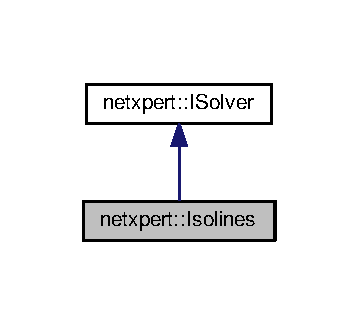
\includegraphics[width=172pt]{classnetxpert_1_1Isolines__inherit__graph}
\end{center}
\end{figure}


Collaboration diagram for netxpert\+:\+:Isolines\+:\nopagebreak
\begin{figure}[H]
\begin{center}
\leavevmode
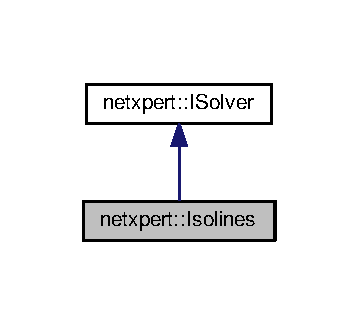
\includegraphics[width=172pt]{classnetxpert_1_1Isolines__coll__graph}
\end{center}
\end{figure}
\subsection*{Public Member Functions}
\begin{DoxyCompactItemize}
\item 
{\bfseries Isolines} (\hyperlink{structnetxpert_1_1cnfg_1_1Config}{netxpert\+::cnfg\+::\+Config} \&cnfg)\hypertarget{classnetxpert_1_1Isolines_acb5bc1dcfd8535cf2382da7bb2fc72e0}{}\label{classnetxpert_1_1Isolines_acb5bc1dcfd8535cf2382da7bb2fc72e0}

\item 
void {\bfseries Solve} (std\+::string net)\hypertarget{classnetxpert_1_1Isolines_ad39fb089dddaa857f16f2a9e1b24ea99}{}\label{classnetxpert_1_1Isolines_ad39fb089dddaa857f16f2a9e1b24ea99}

\item 
void {\bfseries Solve} (\hyperlink{classnetxpert_1_1InternalNet}{netxpert\+::\+Internal\+Net} \&net)\hypertarget{classnetxpert_1_1Isolines_a5d079814c4ed89bd44e4325f0bd98ec4}{}\label{classnetxpert_1_1Isolines_a5d079814c4ed89bd44e4325f0bd98ec4}

\item 
\hyperlink{namespacenetxpert_1_1cnfg_a6ff755ed7f76e0049e3eeeed86c9b55d}{netxpert\+::cnfg\+::\+S\+P\+T\+Algorithm} {\bfseries Get\+Algorithm} () const \hypertarget{classnetxpert_1_1Isolines_a760a64b82f9861b02307628c77834951}{}\label{classnetxpert_1_1Isolines_a760a64b82f9861b02307628c77834951}

\item 
void {\bfseries Set\+Algorithm} (\hyperlink{namespacenetxpert_1_1cnfg_a6ff755ed7f76e0049e3eeeed86c9b55d}{netxpert\+::cnfg\+::\+S\+P\+T\+Algorithm} mst\+Algorithm)\hypertarget{classnetxpert_1_1Isolines_a5bab8b9300026387a4b654783182c7bb}{}\label{classnetxpert_1_1Isolines_a5bab8b9300026387a4b654783182c7bb}

\item 
int {\bfseries Get\+S\+P\+T\+Heap\+Card} () const \hypertarget{classnetxpert_1_1Isolines_a472e713ce884e0a52cbc965ea5c88bb0}{}\label{classnetxpert_1_1Isolines_a472e713ce884e0a52cbc965ea5c88bb0}

\item 
void {\bfseries Set\+S\+P\+T\+Heap\+Card} (int heap\+Card)\hypertarget{classnetxpert_1_1Isolines_a723ac49d853072e88ea3aa56804ae8e1}{}\label{classnetxpert_1_1Isolines_a723ac49d853072e88ea3aa56804ae8e1}

\item 
\hyperlink{namespacenetxpert_1_1cnfg_a1514d3ae51414bf0bcd8d1fe8e868b89}{netxpert\+::cnfg\+::\+G\+E\+O\+M\+E\+T\+R\+Y\+\_\+\+H\+A\+N\+D\+L\+I\+NG} {\bfseries Get\+Geometry\+Handling} () const \hypertarget{classnetxpert_1_1Isolines_abf02c332c26d2d9963fce909124c351f}{}\label{classnetxpert_1_1Isolines_abf02c332c26d2d9963fce909124c351f}

\item 
void {\bfseries Set\+Geometry\+Handling} (\hyperlink{namespacenetxpert_1_1cnfg_a1514d3ae51414bf0bcd8d1fe8e868b89}{netxpert\+::cnfg\+::\+G\+E\+O\+M\+E\+T\+R\+Y\+\_\+\+H\+A\+N\+D\+L\+I\+NG} geom\+Handling)\hypertarget{classnetxpert_1_1Isolines_a4da1c3178b82c9224e96813618881a18}{}\label{classnetxpert_1_1Isolines_a4da1c3178b82c9224e96813618881a18}

\item 
void {\bfseries Set\+Origins} (std\+::vector$<$ netxpert\+::data\+::node\+\_\+t $>$ \&origs)\hypertarget{classnetxpert_1_1Isolines_ab8f7eeafad0d22c4aa22907c6e435b44}{}\label{classnetxpert_1_1Isolines_ab8f7eeafad0d22c4aa22907c6e435b44}

\item 
void \hyperlink{classnetxpert_1_1Isolines_a268f8d2922cc0a95f48255fd185e95dd}{Set\+Origins} (const std\+::vector$<$ uint32\+\_\+t $>$ \&origs)
\item 
std\+::vector$<$ netxpert\+::data\+::node\+\_\+t $>$ {\bfseries Get\+Origins} () const \hypertarget{classnetxpert_1_1Isolines_aa8e03b9b563a9c6e9f38d1715d73be4a}{}\label{classnetxpert_1_1Isolines_aa8e03b9b563a9c6e9f38d1715d73be4a}

\item 
std\+::vector$<$ uint32\+\_\+t $>$ \hyperlink{classnetxpert_1_1Isolines_a8f20bea3e7cb0f0ce5d6e425e96a8453}{Get\+Origin\+I\+Ds} () const 
\item 
std\+::map$<$ netxpert\+::data\+::\+Ext\+Node\+ID, std\+::vector$<$ double $>$ $>$ {\bfseries Get\+Cut\+Offs} ()\hypertarget{classnetxpert_1_1Isolines_a43c9e00fa69a07cc9ed63faf370a7db6}{}\label{classnetxpert_1_1Isolines_a43c9e00fa69a07cc9ed63faf370a7db6}

\item 
void {\bfseries Set\+Cut\+Offs} (std\+::map$<$ netxpert\+::data\+::\+Ext\+Node\+ID, std\+::vector$<$ double $>$ $>$ \&cut\+Offs)\hypertarget{classnetxpert_1_1Isolines_a43a9387e53fc990cab17a32d8a1e43de}{}\label{classnetxpert_1_1Isolines_a43a9387e53fc990cab17a32d8a1e43de}

\item 
const double {\bfseries Get\+Optimum} () const \hypertarget{classnetxpert_1_1Isolines_a83ed59ee0cab81a47819079daef06659}{}\label{classnetxpert_1_1Isolines_a83ed59ee0cab81a47819079daef06659}

\item 
void {\bfseries Save\+Results} (const std\+::string \&result\+Table\+Name, const \hyperlink{structnetxpert_1_1data_1_1ColumnMap}{netxpert\+::data\+::\+Column\+Map} \&cmap) const \hypertarget{classnetxpert_1_1Isolines_aded20cf087ab22f36a7c718c5b0231c9}{}\label{classnetxpert_1_1Isolines_aded20cf087ab22f36a7c718c5b0231c9}

\item 
std\+::map$<$ \hyperlink{structnetxpert_1_1data_1_1ODPair}{netxpert\+::data\+::\+O\+D\+Pair}, \hyperlink{namespacenetxpert_1_1data_a82e488b55f222a9759d73e24f6087033}{netxpert\+::data\+::\+Compressed\+Path} $>$ {\bfseries Get\+Shortest\+Paths} () const \hypertarget{classnetxpert_1_1Isolines_aa3dcc219417cd639dfc0ef3b65a31dae}{}\label{classnetxpert_1_1Isolines_aa3dcc219417cd639dfc0ef3b65a31dae}

\end{DoxyCompactItemize}


\subsection{Detailed Description}
Solver for calculating \hyperlink{classnetxpert_1_1Isolines}{Isolines}, i.\+e. bands of accessible areas in a network. 

\begin{DoxyWarning}{Warning}
Experimental!
\end{DoxyWarning}
Concept\+: solve the 1 -\/ all S\+PT problem and cut off the routes at the defined cut off values; do this for all origins. 

\subsection{Member Function Documentation}
\index{netxpert\+::\+Isolines@{netxpert\+::\+Isolines}!Get\+Origin\+I\+Ds@{Get\+Origin\+I\+Ds}}
\index{Get\+Origin\+I\+Ds@{Get\+Origin\+I\+Ds}!netxpert\+::\+Isolines@{netxpert\+::\+Isolines}}
\subsubsection[{\texorpdfstring{Get\+Origin\+I\+Ds() const }{GetOriginIDs() const }}]{\setlength{\rightskip}{0pt plus 5cm}std\+::vector$<$uint32\+\_\+t$>$ netxpert\+::\+Isolines\+::\+Get\+Origin\+I\+Ds (
\begin{DoxyParamCaption}
{}
\end{DoxyParamCaption}
) const\hspace{0.3cm}{\ttfamily [inline]}}\hypertarget{classnetxpert_1_1Isolines_a8f20bea3e7cb0f0ce5d6e425e96a8453}{}\label{classnetxpert_1_1Isolines_a8f20bea3e7cb0f0ce5d6e425e96a8453}
Simple Wrapper for S\+W\+IG \index{netxpert\+::\+Isolines@{netxpert\+::\+Isolines}!Set\+Origins@{Set\+Origins}}
\index{Set\+Origins@{Set\+Origins}!netxpert\+::\+Isolines@{netxpert\+::\+Isolines}}
\subsubsection[{\texorpdfstring{Set\+Origins(const std\+::vector$<$ uint32\+\_\+t $>$ \&origs)}{SetOrigins(const std::vector< uint32_t > &origs)}}]{\setlength{\rightskip}{0pt plus 5cm}void netxpert\+::\+Isolines\+::\+Set\+Origins (
\begin{DoxyParamCaption}
\item[{const std\+::vector$<$ uint32\+\_\+t $>$ \&}]{origs}
\end{DoxyParamCaption}
)\hspace{0.3cm}{\ttfamily [inline]}}\hypertarget{classnetxpert_1_1Isolines_a268f8d2922cc0a95f48255fd185e95dd}{}\label{classnetxpert_1_1Isolines_a268f8d2922cc0a95f48255fd185e95dd}
Simple Wrapper for S\+W\+IG 

The documentation for this class was generated from the following file\+:\begin{DoxyCompactItemize}
\item 
/home/hahne/dev/netxpert1\+\_\+0/include/solver/isolines.\+h\end{DoxyCompactItemize}

\hypertarget{classnetxpert_1_1ISolver}{}\section{netxpert\+:\+:I\+Solver Class Reference}
\label{classnetxpert_1_1ISolver}\index{netxpert\+::\+I\+Solver@{netxpert\+::\+I\+Solver}}


Abstract \hyperlink{classClass}{Class} (Interface) for all Solvers.  




{\ttfamily \#include $<$isolver.\+h$>$}



Inheritance diagram for netxpert\+:\+:I\+Solver\+:\nopagebreak
\begin{figure}[H]
\begin{center}
\leavevmode
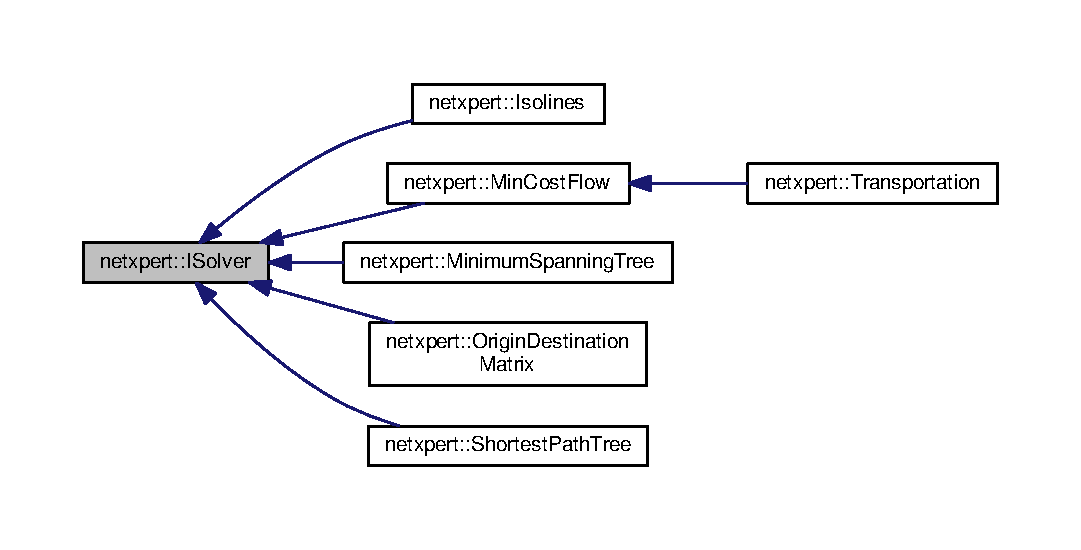
\includegraphics[width=350pt]{classnetxpert_1_1ISolver__inherit__graph}
\end{center}
\end{figure}
\subsection*{Public Member Functions}
\begin{DoxyCompactItemize}
\item 
virtual \hyperlink{classnetxpert_1_1ISolver_adb78f899fbaec49ffd6df5bfd0528074}{$\sim$\+I\+Solver} ()
\item 
virtual void {\bfseries Solve} (std\+::string net)=0\hypertarget{classnetxpert_1_1ISolver_a7b7b8a1f684b832f33bab453020b1b4d}{}\label{classnetxpert_1_1ISolver_a7b7b8a1f684b832f33bab453020b1b4d}

\item 
virtual void {\bfseries Solve} (\hyperlink{classnetxpert_1_1InternalNet}{netxpert\+::\+Internal\+Net} \&net)=0\hypertarget{classnetxpert_1_1ISolver_aaa10dfba4e9fa72426ce15c925cd9176}{}\label{classnetxpert_1_1ISolver_aaa10dfba4e9fa72426ce15c925cd9176}

\item 
virtual const double {\bfseries Get\+Optimum} () const =0\hypertarget{classnetxpert_1_1ISolver_a234f67574e3402388046b224497c9c1e}{}\label{classnetxpert_1_1ISolver_a234f67574e3402388046b224497c9c1e}

\end{DoxyCompactItemize}


\subsection{Detailed Description}
Abstract \hyperlink{classClass}{Class} (Interface) for all Solvers. 

\subsection{Constructor \& Destructor Documentation}
\index{netxpert\+::\+I\+Solver@{netxpert\+::\+I\+Solver}!````~I\+Solver@{$\sim$\+I\+Solver}}
\index{````~I\+Solver@{$\sim$\+I\+Solver}!netxpert\+::\+I\+Solver@{netxpert\+::\+I\+Solver}}
\subsubsection[{\texorpdfstring{$\sim$\+I\+Solver()}{~ISolver()}}]{\setlength{\rightskip}{0pt plus 5cm}virtual netxpert\+::\+I\+Solver\+::$\sim$\+I\+Solver (
\begin{DoxyParamCaption}
{}
\end{DoxyParamCaption}
)\hspace{0.3cm}{\ttfamily [inline]}, {\ttfamily [virtual]}}\hypertarget{classnetxpert_1_1ISolver_adb78f899fbaec49ffd6df5bfd0528074}{}\label{classnetxpert_1_1ISolver_adb78f899fbaec49ffd6df5bfd0528074}
Default destructor 

The documentation for this class was generated from the following file\+:\begin{DoxyCompactItemize}
\item 
/home/hahne/dev/netxpert1\+\_\+0/include/solver/isolver.\+h\end{DoxyCompactItemize}

\hypertarget{classnetxpert_1_1core_1_1ISPTree}{}\section{netxpert\+:\+:core\+:\+:I\+S\+P\+Tree Class Reference}
\label{classnetxpert_1_1core_1_1ISPTree}\index{netxpert\+::core\+::\+I\+S\+P\+Tree@{netxpert\+::core\+::\+I\+S\+P\+Tree}}


Abstract \hyperlink{classClass}{Class} (Interface) for all Shortest Path Tree Solvers in netxpert core.  




{\ttfamily \#include $<$isptree.\+h$>$}



Inheritance diagram for netxpert\+:\+:core\+:\+:I\+S\+P\+Tree\+:\nopagebreak
\begin{figure}[H]
\begin{center}
\leavevmode
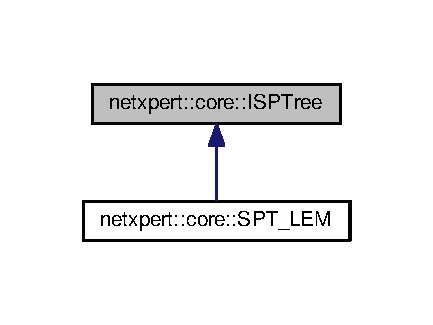
\includegraphics[width=208pt]{classnetxpert_1_1core_1_1ISPTree__inherit__graph}
\end{center}
\end{figure}
\subsection*{Public Member Functions}
\begin{DoxyCompactItemize}
\item 
virtual \hyperlink{classnetxpert_1_1core_1_1ISPTree_a7b61aa12791f75c6979e15f59638cd66}{$\sim$\+I\+S\+P\+Tree} ()
\item 
virtual void {\bfseries Load\+Net} (const uint32\+\_\+t nmax, const uint32\+\_\+t mmax, lemon\+::\+Filter\+Arcs$<$ netxpert\+::data\+::graph\+\_\+t, netxpert\+::data\+::graph\+\_\+t\+::\+Arc\+Map$<$ bool $>$$>$ $\ast$sg, netxpert\+::data\+::graph\+\_\+t\+::\+Arc\+Map$<$ netxpert\+::data\+::cost\+\_\+t $>$ $\ast$cm)=0\hypertarget{classnetxpert_1_1core_1_1ISPTree_a0f402198fc211009404778f75fa2d7cd}{}\label{classnetxpert_1_1core_1_1ISPTree_a0f402198fc211009404778f75fa2d7cd}

\item 
virtual const uint32\+\_\+t {\bfseries Get\+Arc\+Count} ()=0\hypertarget{classnetxpert_1_1core_1_1ISPTree_a55c963bcf6487959df59aa16cef0ea09}{}\label{classnetxpert_1_1core_1_1ISPTree_a55c963bcf6487959df59aa16cef0ea09}

\item 
virtual const uint32\+\_\+t {\bfseries Get\+Node\+Count} ()=0\hypertarget{classnetxpert_1_1core_1_1ISPTree_abe34ece0cc4fb8033d19cbb40b771e27}{}\label{classnetxpert_1_1core_1_1ISPTree_abe34ece0cc4fb8033d19cbb40b771e27}

\item 
virtual void {\bfseries Solve\+S\+PT} (netxpert\+::data\+::cost\+\_\+t treshold=-\/1, bool bidirectional=false)=0\hypertarget{classnetxpert_1_1core_1_1ISPTree_a2db289365cb0d26a1383cb597fd33c64}{}\label{classnetxpert_1_1core_1_1ISPTree_a2db289365cb0d26a1383cb597fd33c64}

\item 
virtual void {\bfseries Set\+Origin} (netxpert\+::data\+::node\+\_\+t New\+Org)=0\hypertarget{classnetxpert_1_1core_1_1ISPTree_a61eac5ae182237609500301be61be3fc}{}\label{classnetxpert_1_1core_1_1ISPTree_a61eac5ae182237609500301be61be3fc}

\item 
virtual void {\bfseries Set\+Dest} (netxpert\+::data\+::node\+\_\+t New\+Dst)=0\hypertarget{classnetxpert_1_1core_1_1ISPTree_a6b7b96b53e27888109e5c97d327e96fc}{}\label{classnetxpert_1_1core_1_1ISPTree_a6b7b96b53e27888109e5c97d327e96fc}

\item 
virtual bool {\bfseries Reached} (netxpert\+::data\+::node\+\_\+t Node\+ID)=0\hypertarget{classnetxpert_1_1core_1_1ISPTree_adfa7078d4e790f10090d67a7f50f1b0d}{}\label{classnetxpert_1_1core_1_1ISPTree_adfa7078d4e790f10090d67a7f50f1b0d}

\item 
virtual const std\+::vector$<$ netxpert\+::data\+::node\+\_\+t $>$ {\bfseries Get\+Predecessors} (netxpert\+::data\+::node\+\_\+t \+\_\+dest)=0\hypertarget{classnetxpert_1_1core_1_1ISPTree_a7aee1d7f478bf851fd04df7484484c51}{}\label{classnetxpert_1_1core_1_1ISPTree_a7aee1d7f478bf851fd04df7484484c51}

\item 
virtual const std\+::vector$<$ netxpert\+::data\+::arc\+\_\+t $>$ {\bfseries Get\+Path} (netxpert\+::data\+::node\+\_\+t \+\_\+dest)=0\hypertarget{classnetxpert_1_1core_1_1ISPTree_ac3f4413acee44b24e594ae1a5444f7b3}{}\label{classnetxpert_1_1core_1_1ISPTree_ac3f4413acee44b24e594ae1a5444f7b3}

\item 
virtual const netxpert\+::data\+::cost\+\_\+t {\bfseries Get\+Dist} (netxpert\+::data\+::node\+\_\+t \+\_\+dest)=0\hypertarget{classnetxpert_1_1core_1_1ISPTree_ad8f1456e940781da2cc414634fe584b8}{}\label{classnetxpert_1_1core_1_1ISPTree_ad8f1456e940781da2cc414634fe584b8}

\end{DoxyCompactItemize}


\subsection{Detailed Description}
Abstract \hyperlink{classClass}{Class} (Interface) for all Shortest Path Tree Solvers in netxpert core. 

\subsection{Constructor \& Destructor Documentation}
\index{netxpert\+::core\+::\+I\+S\+P\+Tree@{netxpert\+::core\+::\+I\+S\+P\+Tree}!````~I\+S\+P\+Tree@{$\sim$\+I\+S\+P\+Tree}}
\index{````~I\+S\+P\+Tree@{$\sim$\+I\+S\+P\+Tree}!netxpert\+::core\+::\+I\+S\+P\+Tree@{netxpert\+::core\+::\+I\+S\+P\+Tree}}
\subsubsection[{\texorpdfstring{$\sim$\+I\+S\+P\+Tree()}{~ISPTree()}}]{\setlength{\rightskip}{0pt plus 5cm}virtual netxpert\+::core\+::\+I\+S\+P\+Tree\+::$\sim$\+I\+S\+P\+Tree (
\begin{DoxyParamCaption}
{}
\end{DoxyParamCaption}
)\hspace{0.3cm}{\ttfamily [inline]}, {\ttfamily [virtual]}}\hypertarget{classnetxpert_1_1core_1_1ISPTree_a7b61aa12791f75c6979e15f59638cd66}{}\label{classnetxpert_1_1core_1_1ISPTree_a7b61aa12791f75c6979e15f59638cd66}
Default destructor 

The documentation for this class was generated from the following file\+:\begin{DoxyCompactItemize}
\item 
/home/hahne/dev/netxpert1\+\_\+0/include/core/isptree.\+h\end{DoxyCompactItemize}

\hypertarget{classnetxpert_1_1utils_1_1LOGGER}{}\section{netxpert\+:\+:utils\+:\+:L\+O\+G\+G\+ER Class Reference}
\label{classnetxpert_1_1utils_1_1LOGGER}\index{netxpert\+::utils\+::\+L\+O\+G\+G\+ER@{netxpert\+::utils\+::\+L\+O\+G\+G\+ER}}


Logger class.  




{\ttfamily \#include $<$logger.\+h$>$}

\subsection*{Static Public Member Functions}
\begin{DoxyCompactItemize}
\item 
static void {\bfseries Initialize} (const \hyperlink{structnetxpert_1_1cnfg_1_1Config}{netxpert\+::cnfg\+::\+Config} \&cnfg)\hypertarget{classnetxpert_1_1utils_1_1LOGGER_ad122b92cee3035750ea187afc31d13d8}{}\label{classnetxpert_1_1utils_1_1LOGGER_ad122b92cee3035750ea187afc31d13d8}

\item 
static void {\bfseries Log\+Debug} (std\+::string log\+Msg)\hypertarget{classnetxpert_1_1utils_1_1LOGGER_aa9150ff82d540dbdd39f90e8f4690ba6}{}\label{classnetxpert_1_1utils_1_1LOGGER_aa9150ff82d540dbdd39f90e8f4690ba6}

\item 
static void {\bfseries Log\+Info} (std\+::string log\+Msg)\hypertarget{classnetxpert_1_1utils_1_1LOGGER_a1e480b4dc6a33bca4e6a732e018841a9}{}\label{classnetxpert_1_1utils_1_1LOGGER_a1e480b4dc6a33bca4e6a732e018841a9}

\item 
static void {\bfseries Log\+Warning} (std\+::string log\+Msg)\hypertarget{classnetxpert_1_1utils_1_1LOGGER_a184af8779965d8663ca84b4f7e4ba3e9}{}\label{classnetxpert_1_1utils_1_1LOGGER_a184af8779965d8663ca84b4f7e4ba3e9}

\item 
static void {\bfseries Log\+Error} (std\+::string log\+Msg)\hypertarget{classnetxpert_1_1utils_1_1LOGGER_af336fd2d432bf26747590f3a3a5a92c3}{}\label{classnetxpert_1_1utils_1_1LOGGER_af336fd2d432bf26747590f3a3a5a92c3}

\item 
static void {\bfseries Log\+Fatal} (std\+::string log\+Msg)\hypertarget{classnetxpert_1_1utils_1_1LOGGER_aea1f7109666d88ce88e7612494ee59f1}{}\label{classnetxpert_1_1utils_1_1LOGGER_aea1f7109666d88ce88e7612494ee59f1}

\end{DoxyCompactItemize}
\subsection*{Static Public Attributes}
\begin{DoxyCompactItemize}
\item 
static bool {\bfseries Is\+Initialized}\hypertarget{classnetxpert_1_1utils_1_1LOGGER_a7577f62a660b9897d686cdfe88ae441d}{}\label{classnetxpert_1_1utils_1_1LOGGER_a7577f62a660b9897d686cdfe88ae441d}

\item 
static std\+::string {\bfseries Full\+Log\+File\+Name}\hypertarget{classnetxpert_1_1utils_1_1LOGGER_a8235454671e8ef5030e271479a01e0f7}{}\label{classnetxpert_1_1utils_1_1LOGGER_a8235454671e8ef5030e271479a01e0f7}

\end{DoxyCompactItemize}


\subsection{Detailed Description}
Logger class. 

The documentation for this class was generated from the following file\+:\begin{DoxyCompactItemize}
\item 
/home/hahne/dev/netxpert1\+\_\+0/include/logger.\+h\end{DoxyCompactItemize}

\hypertarget{classnetxpert_1_1simple_1_1MinCostFlow}{}\section{netxpert\+:\+:simple\+:\+:Min\+Cost\+Flow Class Reference}
\label{classnetxpert_1_1simple_1_1MinCostFlow}\index{netxpert\+::simple\+::\+Min\+Cost\+Flow@{netxpert\+::simple\+::\+Min\+Cost\+Flow}}
\subsection*{Public Member Functions}
\begin{DoxyCompactItemize}
\item 
{\bfseries Min\+Cost\+Flow} (std\+::string json\+Cnfg)\hypertarget{classnetxpert_1_1simple_1_1MinCostFlow_a13dfb61a02a2f888020466eb2598b40e}{}\label{classnetxpert_1_1simple_1_1MinCostFlow_a13dfb61a02a2f888020466eb2598b40e}

\item 
int {\bfseries Solve} ()\hypertarget{classnetxpert_1_1simple_1_1MinCostFlow_a9dc858a93393ef31b2c91b81a0d820f9}{}\label{classnetxpert_1_1simple_1_1MinCostFlow_a9dc858a93393ef31b2c91b81a0d820f9}

\item 
double {\bfseries Get\+Optimum} ()\hypertarget{classnetxpert_1_1simple_1_1MinCostFlow_acc572dba96f07653eb3ca0d84256b401}{}\label{classnetxpert_1_1simple_1_1MinCostFlow_acc572dba96f07653eb3ca0d84256b401}

\item 
std\+::string {\bfseries Get\+Minimum\+Cost\+Flow\+As\+J\+S\+ON} ()\hypertarget{classnetxpert_1_1simple_1_1MinCostFlow_a02be05d9010997ea763351921baef1fd}{}\label{classnetxpert_1_1simple_1_1MinCostFlow_a02be05d9010997ea763351921baef1fd}

\item 
std\+::vector$<$ \hyperlink{structnetxpert_1_1data_1_1FlowCost}{netxpert\+::data\+::\+Flow\+Cost} $>$ {\bfseries Get\+Minimum\+Cost\+Flow} ()\hypertarget{classnetxpert_1_1simple_1_1MinCostFlow_a8281df731a9a267ad58104fed3f6fa82}{}\label{classnetxpert_1_1simple_1_1MinCostFlow_a8281df731a9a267ad58104fed3f6fa82}

\end{DoxyCompactItemize}


The documentation for this class was generated from the following file\+:\begin{DoxyCompactItemize}
\item 
/home/hahne/dev/netxpert1\+\_\+0/include/simple/mcfp\+\_\+simple.\+h\end{DoxyCompactItemize}

\hypertarget{classnetxpert_1_1MinCostFlow}{}\section{netxpert\+:\+:Min\+Cost\+Flow Class Reference}
\label{classnetxpert_1_1MinCostFlow}\index{netxpert\+::\+Min\+Cost\+Flow@{netxpert\+::\+Min\+Cost\+Flow}}


Solver for the Minimum Cost Flow Problem.  




{\ttfamily \#include $<$mcflow.\+h$>$}



Inheritance diagram for netxpert\+:\+:Min\+Cost\+Flow\+:\nopagebreak
\begin{figure}[H]
\begin{center}
\leavevmode
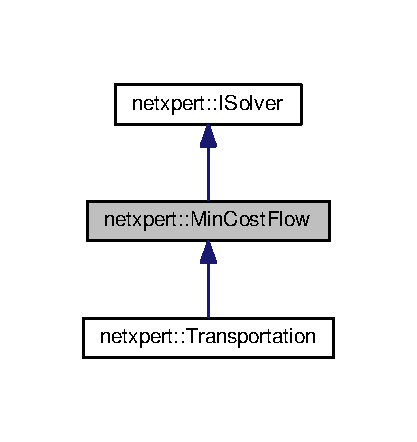
\includegraphics[width=200pt]{classnetxpert_1_1MinCostFlow__inherit__graph}
\end{center}
\end{figure}


Collaboration diagram for netxpert\+:\+:Min\+Cost\+Flow\+:\nopagebreak
\begin{figure}[H]
\begin{center}
\leavevmode
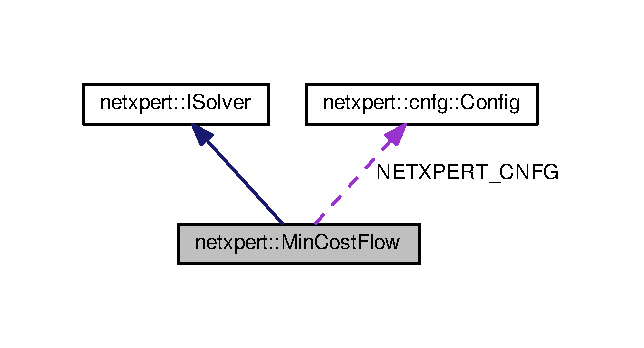
\includegraphics[width=309pt]{classnetxpert_1_1MinCostFlow__coll__graph}
\end{center}
\end{figure}
\subsection*{Public Member Functions}
\begin{DoxyCompactItemize}
\item 
{\bfseries Min\+Cost\+Flow} (\hyperlink{structnetxpert_1_1cnfg_1_1Config}{netxpert\+::cnfg\+::\+Config} \&cnfg)\hypertarget{classnetxpert_1_1MinCostFlow_ac130d7426b4d84a02373e51454fdc63f}{}\label{classnetxpert_1_1MinCostFlow_ac130d7426b4d84a02373e51454fdc63f}

\item 
void {\bfseries Solve} (std\+::string net)\hypertarget{classnetxpert_1_1MinCostFlow_a818d05c0b2b1e517e65b7670c3e3ad75}{}\label{classnetxpert_1_1MinCostFlow_a818d05c0b2b1e517e65b7670c3e3ad75}

\item 
void {\bfseries Solve} (\hyperlink{classnetxpert_1_1InternalNet}{netxpert\+::\+Internal\+Net} \&net)\hypertarget{classnetxpert_1_1MinCostFlow_a62aeea837ffdb2c659a0ac741d64137b}{}\label{classnetxpert_1_1MinCostFlow_a62aeea837ffdb2c659a0ac741d64137b}

\item 
std\+::vector$<$ \hyperlink{structnetxpert_1_1data_1_1FlowCost}{netxpert\+::data\+::\+Flow\+Cost} $>$ {\bfseries Get\+Min\+Cost\+Flow} () const \hypertarget{classnetxpert_1_1MinCostFlow_a245a11fd055d104bade19bc44ca415d5}{}\label{classnetxpert_1_1MinCostFlow_a245a11fd055d104bade19bc44ca415d5}

\item 
\hyperlink{namespacenetxpert_1_1cnfg_aae922390a89b0c9af1bc2532428c5ef9}{netxpert\+::cnfg\+::\+M\+C\+F\+Algorithm} {\bfseries Get\+Algorithm} () const \hypertarget{classnetxpert_1_1MinCostFlow_acca2bc1d079cf8de208fffb02a92a49f}{}\label{classnetxpert_1_1MinCostFlow_acca2bc1d079cf8de208fffb02a92a49f}

\item 
void {\bfseries Set\+Algorithm} (\hyperlink{namespacenetxpert_1_1cnfg_aae922390a89b0c9af1bc2532428c5ef9}{netxpert\+::cnfg\+::\+M\+C\+F\+Algorithm} mcf\+Algorithm)\hypertarget{classnetxpert_1_1MinCostFlow_abf6a79a9451ae557338fb72c29813897}{}\label{classnetxpert_1_1MinCostFlow_abf6a79a9451ae557338fb72c29813897}

\item 
\hyperlink{namespacenetxpert_1_1data_a0ea30f651c6cc7e7a6edd5a5cbe6346c}{netxpert\+::data\+::\+M\+C\+F\+Solver\+Status} {\bfseries Get\+Solver\+Status} () const \hypertarget{classnetxpert_1_1MinCostFlow_ab87f6c58a8173823296fcb3529947495}{}\label{classnetxpert_1_1MinCostFlow_ab87f6c58a8173823296fcb3529947495}

\item 
const double {\bfseries Get\+Optimum} () const \hypertarget{classnetxpert_1_1MinCostFlow_ab4201f39d97364c9b0766b2c4f6415b0}{}\label{classnetxpert_1_1MinCostFlow_ab4201f39d97364c9b0766b2c4f6415b0}

\item 
void {\bfseries Save\+Results} (const std\+::string \&result\+Table\+Name, const \hyperlink{structnetxpert_1_1data_1_1ColumnMap}{netxpert\+::data\+::\+Column\+Map} \&cmap) const \hypertarget{classnetxpert_1_1MinCostFlow_a8f0f6280d112e40d2215dcba35022ef5}{}\label{classnetxpert_1_1MinCostFlow_a8f0f6280d112e40d2215dcba35022ef5}

\end{DoxyCompactItemize}
\subsection*{Public Attributes}
\begin{DoxyCompactItemize}
\item 
bool {\bfseries Is\+Directed}\hypertarget{classnetxpert_1_1MinCostFlow_ac9f9eec0385917e499121a44a7a5cc7c}{}\label{classnetxpert_1_1MinCostFlow_ac9f9eec0385917e499121a44a7a5cc7c}

\end{DoxyCompactItemize}
\subsection*{Protected Member Functions}
\begin{DoxyCompactItemize}
\item 
void {\bfseries solve} (\hyperlink{classnetxpert_1_1InternalNet}{netxpert\+::\+Internal\+Net} \&net)\hypertarget{classnetxpert_1_1MinCostFlow_aa488ec0d0eb1b492bae093ae3cec7040}{}\label{classnetxpert_1_1MinCostFlow_aa488ec0d0eb1b492bae093ae3cec7040}

\item 
bool {\bfseries validate\+Network\+Data} (\hyperlink{classnetxpert_1_1InternalNet}{netxpert\+::\+Internal\+Net} \&net)\hypertarget{classnetxpert_1_1MinCostFlow_a30d7985e7f5149476c3442146204f709}{}\label{classnetxpert_1_1MinCostFlow_a30d7985e7f5149476c3442146204f709}

\item 
lemon\+::\+Filter\+Arcs$<$ netxpert\+::data\+::graph\+\_\+t, netxpert\+::data\+::graph\+\_\+t\+::\+Arc\+Map$<$ bool $>$ $>$ {\bfseries convert\+Internal\+Network\+To\+Solver\+Data} (\hyperlink{classnetxpert_1_1InternalNet}{netxpert\+::\+Internal\+Net} \&net)\hypertarget{classnetxpert_1_1MinCostFlow_a87acb5c57d7c13dc4ce87751bd112d30}{}\label{classnetxpert_1_1MinCostFlow_a87acb5c57d7c13dc4ce87751bd112d30}

\item 
void {\bfseries get\+Supply\+Nodes\+Type\+Count} (int \&src\+Node\+Count, int \&transship\+Node\+Count, int \&sink\+Node\+Count)\hypertarget{classnetxpert_1_1MinCostFlow_af43ab101328511e444adac86b25076f6}{}\label{classnetxpert_1_1MinCostFlow_af43ab101328511e444adac86b25076f6}

\end{DoxyCompactItemize}
\subsection*{Protected Attributes}
\begin{DoxyCompactItemize}
\item 
\hyperlink{structnetxpert_1_1cnfg_1_1Config}{netxpert\+::cnfg\+::\+Config} {\bfseries N\+E\+T\+X\+P\+E\+R\+T\+\_\+\+C\+N\+FG}\hypertarget{classnetxpert_1_1MinCostFlow_a7eb616387e700481e8bd38d0895a0b0c}{}\label{classnetxpert_1_1MinCostFlow_a7eb616387e700481e8bd38d0895a0b0c}

\item 
double {\bfseries optimum} = 0\hypertarget{classnetxpert_1_1MinCostFlow_ac97c5e0f6fea8cbb91ca6a1ee20a19ae}{}\label{classnetxpert_1_1MinCostFlow_ac97c5e0f6fea8cbb91ca6a1ee20a19ae}

\item 
\hyperlink{namespacenetxpert_1_1data_a0ea30f651c6cc7e7a6edd5a5cbe6346c}{netxpert\+::data\+::\+M\+C\+F\+Solver\+Status} {\bfseries solver\+Status}\hypertarget{classnetxpert_1_1MinCostFlow_a9a48b11bac35b930a4b6445fbf49e1ca}{}\label{classnetxpert_1_1MinCostFlow_a9a48b11bac35b930a4b6445fbf49e1ca}

\item 
\hyperlink{namespacenetxpert_1_1cnfg_aae922390a89b0c9af1bc2532428c5ef9}{netxpert\+::cnfg\+::\+M\+C\+F\+Algorithm} {\bfseries algorithm}\hypertarget{classnetxpert_1_1MinCostFlow_af32c8684a78aecf05eca2284a143ab7b}{}\label{classnetxpert_1_1MinCostFlow_af32c8684a78aecf05eca2284a143ab7b}

\item 
std\+::vector$<$ \hyperlink{structnetxpert_1_1data_1_1FlowCost}{netxpert\+::data\+::\+Flow\+Cost} $>$ {\bfseries flow\+Cost}\hypertarget{classnetxpert_1_1MinCostFlow_acb4f44eae2cd34f6bb759e38020f5caf}{}\label{classnetxpert_1_1MinCostFlow_acb4f44eae2cd34f6bb759e38020f5caf}

\item 
std\+::shared\+\_\+ptr$<$ \hyperlink{classnetxpert_1_1core_1_1IMinCostFlow}{netxpert\+::core\+::\+I\+Min\+Cost\+Flow} $>$ {\bfseries mcf}\hypertarget{classnetxpert_1_1MinCostFlow_acb8876e53342acf0f90a009ba7766935}{}\label{classnetxpert_1_1MinCostFlow_acb8876e53342acf0f90a009ba7766935}

\end{DoxyCompactItemize}


\subsection{Detailed Description}
Solver for the Minimum Cost Flow Problem. 

The documentation for this class was generated from the following file\+:\begin{DoxyCompactItemize}
\item 
/home/hahne/dev/netxpert1\+\_\+0/include/solver/mcflow.\+h\end{DoxyCompactItemize}

\hypertarget{classnetxpert_1_1MinimumSpanningTree}{}\section{netxpert\+:\+:Minimum\+Spanning\+Tree Class Reference}
\label{classnetxpert_1_1MinimumSpanningTree}\index{netxpert\+::\+Minimum\+Spanning\+Tree@{netxpert\+::\+Minimum\+Spanning\+Tree}}


Solver for the Minimum Spanning Tree Problem.  




{\ttfamily \#include $<$mstree.\+h$>$}



Inheritance diagram for netxpert\+:\+:Minimum\+Spanning\+Tree\+:\nopagebreak
\begin{figure}[H]
\begin{center}
\leavevmode
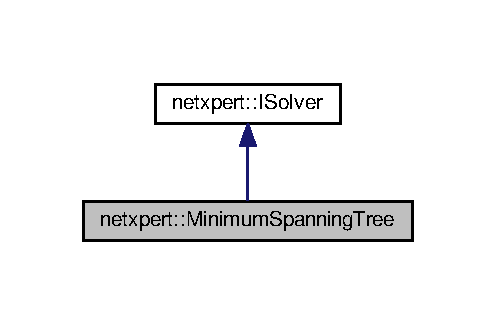
\includegraphics[width=238pt]{classnetxpert_1_1MinimumSpanningTree__inherit__graph}
\end{center}
\end{figure}


Collaboration diagram for netxpert\+:\+:Minimum\+Spanning\+Tree\+:\nopagebreak
\begin{figure}[H]
\begin{center}
\leavevmode
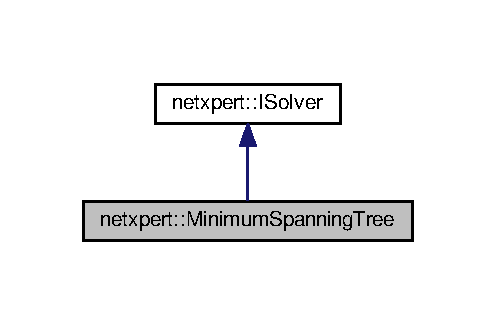
\includegraphics[width=238pt]{classnetxpert_1_1MinimumSpanningTree__coll__graph}
\end{center}
\end{figure}
\subsection*{Public Member Functions}
\begin{DoxyCompactItemize}
\item 
\hyperlink{classnetxpert_1_1MinimumSpanningTree_a7d1cd0fc061bd8b056f4317eabdcdc0a}{Minimum\+Spanning\+Tree} (\hyperlink{structnetxpert_1_1cnfg_1_1Config}{netxpert\+::cnfg\+::\+Config} \&cnfg)
\item 
\hyperlink{classnetxpert_1_1MinimumSpanningTree_ab3ad88e9f5a29b397de4e55f1ffb12f8}{$\sim$\+Minimum\+Spanning\+Tree} ()
\item 
void {\bfseries Solve} (std\+::string net)\hypertarget{classnetxpert_1_1MinimumSpanningTree_ae7ae3fa3b3be489c9d4de521a93b5afe}{}\label{classnetxpert_1_1MinimumSpanningTree_ae7ae3fa3b3be489c9d4de521a93b5afe}

\item 
void {\bfseries Solve} (\hyperlink{classnetxpert_1_1InternalNet}{netxpert\+::\+Internal\+Net} \&net)\hypertarget{classnetxpert_1_1MinimumSpanningTree_a9feb9c9f9d154da798f079b23f0f81f0}{}\label{classnetxpert_1_1MinimumSpanningTree_a9feb9c9f9d154da798f079b23f0f81f0}

\item 
\hyperlink{namespacenetxpert_1_1cnfg_ab77ff30f2da32945dbb19bdf6199f799}{netxpert\+::cnfg\+::\+M\+S\+T\+Algorithm} {\bfseries Get\+Algorithm} () const \hypertarget{classnetxpert_1_1MinimumSpanningTree_ac3f3aae29b21d63a744337e1a1f3e731}{}\label{classnetxpert_1_1MinimumSpanningTree_ac3f3aae29b21d63a744337e1a1f3e731}

\item 
void {\bfseries Set\+Algorithm} (\hyperlink{namespacenetxpert_1_1cnfg_ab77ff30f2da32945dbb19bdf6199f799}{netxpert\+::cnfg\+::\+M\+S\+T\+Algorithm} mst\+Algorithm)\hypertarget{classnetxpert_1_1MinimumSpanningTree_ab78ec431e6e093d7add8c4cbf2e42ef2}{}\label{classnetxpert_1_1MinimumSpanningTree_ab78ec431e6e093d7add8c4cbf2e42ef2}

\item 
const double {\bfseries Get\+Optimum} () const \hypertarget{classnetxpert_1_1MinimumSpanningTree_a5a8777928028df716efcabd643cf3506}{}\label{classnetxpert_1_1MinimumSpanningTree_a5a8777928028df716efcabd643cf3506}

\item 
std\+::vector$<$ netxpert\+::data\+::arc\+\_\+t $>$ {\bfseries Get\+Minimum\+Spanning\+Tree} () const \hypertarget{classnetxpert_1_1MinimumSpanningTree_a79bb14f2ccab2abcacf9bb466d1e3a1c}{}\label{classnetxpert_1_1MinimumSpanningTree_a79bb14f2ccab2abcacf9bb466d1e3a1c}

\item 
void {\bfseries Save\+Results} (const std\+::string \&result\+Table\+Name, const \hyperlink{structnetxpert_1_1data_1_1ColumnMap}{netxpert\+::data\+::\+Column\+Map} \&cmap) const \hypertarget{classnetxpert_1_1MinimumSpanningTree_a958dacf0024f62a9bd46a4bef28827f7}{}\label{classnetxpert_1_1MinimumSpanningTree_a958dacf0024f62a9bd46a4bef28827f7}

\end{DoxyCompactItemize}


\subsection{Detailed Description}
Solver for the Minimum Spanning Tree Problem. 

\subsection{Constructor \& Destructor Documentation}
\index{netxpert\+::\+Minimum\+Spanning\+Tree@{netxpert\+::\+Minimum\+Spanning\+Tree}!Minimum\+Spanning\+Tree@{Minimum\+Spanning\+Tree}}
\index{Minimum\+Spanning\+Tree@{Minimum\+Spanning\+Tree}!netxpert\+::\+Minimum\+Spanning\+Tree@{netxpert\+::\+Minimum\+Spanning\+Tree}}
\subsubsection[{\texorpdfstring{Minimum\+Spanning\+Tree(netxpert\+::cnfg\+::\+Config \&cnfg)}{MinimumSpanningTree(netxpert::cnfg::Config &cnfg)}}]{\setlength{\rightskip}{0pt plus 5cm}netxpert\+::\+Minimum\+Spanning\+Tree\+::\+Minimum\+Spanning\+Tree (
\begin{DoxyParamCaption}
\item[{{\bf netxpert\+::cnfg\+::\+Config} \&}]{cnfg}
\end{DoxyParamCaption}
)}\hypertarget{classnetxpert_1_1MinimumSpanningTree_a7d1cd0fc061bd8b056f4317eabdcdc0a}{}\label{classnetxpert_1_1MinimumSpanningTree_a7d1cd0fc061bd8b056f4317eabdcdc0a}
Default constructor \index{netxpert\+::\+Minimum\+Spanning\+Tree@{netxpert\+::\+Minimum\+Spanning\+Tree}!````~Minimum\+Spanning\+Tree@{$\sim$\+Minimum\+Spanning\+Tree}}
\index{````~Minimum\+Spanning\+Tree@{$\sim$\+Minimum\+Spanning\+Tree}!netxpert\+::\+Minimum\+Spanning\+Tree@{netxpert\+::\+Minimum\+Spanning\+Tree}}
\subsubsection[{\texorpdfstring{$\sim$\+Minimum\+Spanning\+Tree()}{~MinimumSpanningTree()}}]{\setlength{\rightskip}{0pt plus 5cm}netxpert\+::\+Minimum\+Spanning\+Tree\+::$\sim$\+Minimum\+Spanning\+Tree (
\begin{DoxyParamCaption}
{}
\end{DoxyParamCaption}
)\hspace{0.3cm}{\ttfamily [inline]}}\hypertarget{classnetxpert_1_1MinimumSpanningTree_ab3ad88e9f5a29b397de4e55f1ffb12f8}{}\label{classnetxpert_1_1MinimumSpanningTree_ab3ad88e9f5a29b397de4e55f1ffb12f8}
Default destructor 

The documentation for this class was generated from the following file\+:\begin{DoxyCompactItemize}
\item 
/home/hahne/dev/netxpert1\+\_\+0/include/solver/mstree.\+h\end{DoxyCompactItemize}

\hypertarget{classnetxpert_1_1simple_1_1MinimumSpanningTree}{}\section{netxpert\+:\+:simple\+:\+:Minimum\+Spanning\+Tree Class Reference}
\label{classnetxpert_1_1simple_1_1MinimumSpanningTree}\index{netxpert\+::simple\+::\+Minimum\+Spanning\+Tree@{netxpert\+::simple\+::\+Minimum\+Spanning\+Tree}}
\subsection*{Public Member Functions}
\begin{DoxyCompactItemize}
\item 
{\bfseries Minimum\+Spanning\+Tree} (std\+::string json\+Cnfg)\hypertarget{classnetxpert_1_1simple_1_1MinimumSpanningTree_a3f2cdeae5033766a054e20ed2ce02e3b}{}\label{classnetxpert_1_1simple_1_1MinimumSpanningTree_a3f2cdeae5033766a054e20ed2ce02e3b}

\item 
int {\bfseries Solve} ()\hypertarget{classnetxpert_1_1simple_1_1MinimumSpanningTree_abc9cd18efebd7c7fe5e449849f92530f}{}\label{classnetxpert_1_1simple_1_1MinimumSpanningTree_abc9cd18efebd7c7fe5e449849f92530f}

\item 
double {\bfseries Get\+Optimum} ()\hypertarget{classnetxpert_1_1simple_1_1MinimumSpanningTree_a27eb0c623199876d1fdace2c8f32e88b}{}\label{classnetxpert_1_1simple_1_1MinimumSpanningTree_a27eb0c623199876d1fdace2c8f32e88b}

\item 
std\+::string {\bfseries Get\+Minimum\+Spanning\+Tree\+As\+J\+S\+ON} ()\hypertarget{classnetxpert_1_1simple_1_1MinimumSpanningTree_a8200c69b26e1910f2c22ea3842027242}{}\label{classnetxpert_1_1simple_1_1MinimumSpanningTree_a8200c69b26e1910f2c22ea3842027242}

\item 
std\+::vector$<$ \hyperlink{structnetxpert_1_1data_1_1ExternalArc}{netxpert\+::data\+::\+External\+Arc} $>$ {\bfseries Get\+Minimum\+Spanning\+Tree} ()\hypertarget{classnetxpert_1_1simple_1_1MinimumSpanningTree_ad43de6f61435414777307a685b1ad46b}{}\label{classnetxpert_1_1simple_1_1MinimumSpanningTree_ad43de6f61435414777307a685b1ad46b}

\end{DoxyCompactItemize}


The documentation for this class was generated from the following file\+:\begin{DoxyCompactItemize}
\item 
/home/hahne/dev/netxpert1\+\_\+0/include/simple/mstree\+\_\+simple.\+h\end{DoxyCompactItemize}

\hypertarget{classnetxpert_1_1core_1_1MST__LEM}{}\section{netxpert\+:\+:core\+:\+:M\+S\+T\+\_\+\+L\+EM Class Reference}
\label{classnetxpert_1_1core_1_1MST__LEM}\index{netxpert\+::core\+::\+M\+S\+T\+\_\+\+L\+EM@{netxpert\+::core\+::\+M\+S\+T\+\_\+\+L\+EM}}


Core Solver for the Minimum Spanning Tree Problem with L\+E\+M\+ON.  




{\ttfamily \#include $<$mstlem.\+h$>$}



Inheritance diagram for netxpert\+:\+:core\+:\+:M\+S\+T\+\_\+\+L\+EM\+:\nopagebreak
\begin{figure}[H]
\begin{center}
\leavevmode
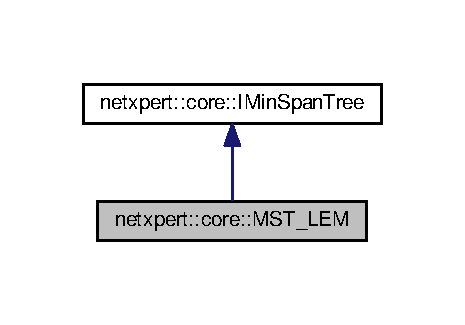
\includegraphics[width=223pt]{classnetxpert_1_1core_1_1MST__LEM__inherit__graph}
\end{center}
\end{figure}


Collaboration diagram for netxpert\+:\+:core\+:\+:M\+S\+T\+\_\+\+L\+EM\+:\nopagebreak
\begin{figure}[H]
\begin{center}
\leavevmode
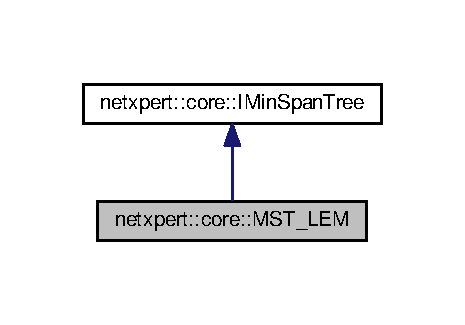
\includegraphics[width=223pt]{classnetxpert_1_1core_1_1MST__LEM__coll__graph}
\end{center}
\end{figure}
\subsection*{Public Member Functions}
\begin{DoxyCompactItemize}
\item 
{\bfseries M\+S\+T\+\_\+\+L\+EM} (\hyperlink{classnetxpert_1_1core_1_1MST__LEM}{M\+S\+T\+\_\+\+L\+EM} const \&)\hypertarget{classnetxpert_1_1core_1_1MST__LEM_abdd5584b9ac0cfbf68ea3053fab84875}{}\label{classnetxpert_1_1core_1_1MST__LEM_abdd5584b9ac0cfbf68ea3053fab84875}

\item 
void {\bfseries Load\+Net} (const uint32\+\_\+t nmax, const uint32\+\_\+t mmax, lemon\+::\+Filter\+Arcs$<$ netxpert\+::data\+::graph\+\_\+t, netxpert\+::data\+::graph\+\_\+t\+::\+Arc\+Map$<$ bool $>$$>$ $\ast$sg, netxpert\+::data\+::graph\+\_\+t\+::\+Arc\+Map$<$ netxpert\+::data\+::cost\+\_\+t $>$ $\ast$cm)\hypertarget{classnetxpert_1_1core_1_1MST__LEM_a5dc785d80fa6ee78d798dbb3f9e61355}{}\label{classnetxpert_1_1core_1_1MST__LEM_a5dc785d80fa6ee78d798dbb3f9e61355}

\item 
const uint32\+\_\+t {\bfseries Get\+Arc\+Count} ()\hypertarget{classnetxpert_1_1core_1_1MST__LEM_a97f75745010d6f4f21f602b59cde87b4}{}\label{classnetxpert_1_1core_1_1MST__LEM_a97f75745010d6f4f21f602b59cde87b4}

\item 
const uint32\+\_\+t {\bfseries Get\+Node\+Count} ()\hypertarget{classnetxpert_1_1core_1_1MST__LEM_a7a3348f7565087a86f156bdd889c6ec8}{}\label{classnetxpert_1_1core_1_1MST__LEM_a7a3348f7565087a86f156bdd889c6ec8}

\item 
void {\bfseries Solve\+M\+ST} ()\hypertarget{classnetxpert_1_1core_1_1MST__LEM_a3aa993c7a865803f7222e7c8d76893e9}{}\label{classnetxpert_1_1core_1_1MST__LEM_a3aa993c7a865803f7222e7c8d76893e9}

\item 
const double {\bfseries Get\+Optimum} () const \hypertarget{classnetxpert_1_1core_1_1MST__LEM_a73b7fa80fae50c424dea2022f45f6ee8}{}\label{classnetxpert_1_1core_1_1MST__LEM_a73b7fa80fae50c424dea2022f45f6ee8}

\item 
std\+::vector$<$ netxpert\+::data\+::arc\+\_\+t $>$ {\bfseries Get\+M\+ST} ()\hypertarget{classnetxpert_1_1core_1_1MST__LEM_afaedc6059124fd068f6db625cc691a32}{}\label{classnetxpert_1_1core_1_1MST__LEM_afaedc6059124fd068f6db625cc691a32}

\end{DoxyCompactItemize}
\subsection*{Protected Attributes}
\begin{DoxyCompactItemize}
\item 
uint32\+\_\+t {\bfseries nmax}\hypertarget{classnetxpert_1_1core_1_1MST__LEM_a3af5cdbf7bdb534934847206ce31fc57}{}\label{classnetxpert_1_1core_1_1MST__LEM_a3af5cdbf7bdb534934847206ce31fc57}

\item 
uint32\+\_\+t {\bfseries mmax}\hypertarget{classnetxpert_1_1core_1_1MST__LEM_ac5d7c2ae33b25ea6c1a8d21c3b899c79}{}\label{classnetxpert_1_1core_1_1MST__LEM_ac5d7c2ae33b25ea6c1a8d21c3b899c79}

\item 
netxpert\+::data\+::filtered\+\_\+graph\+\_\+t $\ast$ {\bfseries g}\hypertarget{classnetxpert_1_1core_1_1MST__LEM_ab62135ef6aa9743fa306cc580f19d0e5}{}\label{classnetxpert_1_1core_1_1MST__LEM_ab62135ef6aa9743fa306cc580f19d0e5}

\item 
netxpert\+::data\+::filtered\+\_\+graph\+\_\+t\+::\+Arc\+Map$<$ bool $>$ $\ast$ {\bfseries arc\+Bool\+Map}\hypertarget{classnetxpert_1_1core_1_1MST__LEM_afa414ca90eeccf83e5788bc6e26a1d93}{}\label{classnetxpert_1_1core_1_1MST__LEM_afa414ca90eeccf83e5788bc6e26a1d93}

\item 
netxpert\+::data\+::graph\+\_\+t\+::\+Arc\+Map$<$ cost\+\_\+t $>$ $\ast$ {\bfseries cost\+Map}\hypertarget{classnetxpert_1_1core_1_1MST__LEM_a879d338b891a8fec4c7b23cd391d87e8}{}\label{classnetxpert_1_1core_1_1MST__LEM_a879d338b891a8fec4c7b23cd391d87e8}

\item 
double {\bfseries total\+Cost}\hypertarget{classnetxpert_1_1core_1_1MST__LEM_a7d1cf08ff7bb320218cdb5feb5f029a7}{}\label{classnetxpert_1_1core_1_1MST__LEM_a7d1cf08ff7bb320218cdb5feb5f029a7}

\item 
std\+::vector$<$ netxpert\+::data\+::node\+\_\+t $>$ {\bfseries nodes}\hypertarget{classnetxpert_1_1core_1_1MST__LEM_a691f128604478290d6d96ed95db14cb2}{}\label{classnetxpert_1_1core_1_1MST__LEM_a691f128604478290d6d96ed95db14cb2}

\end{DoxyCompactItemize}


\subsection{Detailed Description}
Core Solver for the Minimum Spanning Tree Problem with L\+E\+M\+ON. 

The documentation for this class was generated from the following file\+:\begin{DoxyCompactItemize}
\item 
/home/hahne/dev/netxpert1\+\_\+0/include/core/mstlem.\+h\end{DoxyCompactItemize}

\hypertarget{structnetxpert_1_1data_1_1MSTResult}{}\section{netxpert\+:\+:data\+:\+:M\+S\+T\+Result Struct Reference}
\label{structnetxpert_1_1data_1_1MSTResult}\index{netxpert\+::data\+::\+M\+S\+T\+Result@{netxpert\+::data\+::\+M\+S\+T\+Result}}


Data type for storing the result of the M\+ST Solver in J\+S\+O\+N-\/\+Format.  




{\ttfamily \#include $<$data.\+h$>$}

\subsection*{Public Member Functions}
\begin{DoxyCompactItemize}
\item 
{\footnotesize template$<$class Archive $>$ }\\void {\bfseries serialize} (Archive \&ar)\hypertarget{structnetxpert_1_1data_1_1MSTResult_aca4fd1b2be387fb7168fbf6c0b64ba9f}{}\label{structnetxpert_1_1data_1_1MSTResult_aca4fd1b2be387fb7168fbf6c0b64ba9f}

\end{DoxyCompactItemize}
\subsection*{Public Attributes}
\begin{DoxyCompactItemize}
\item 
cost\+\_\+t {\bfseries optimum}\hypertarget{structnetxpert_1_1data_1_1MSTResult_a7e5e35232f019e1652656be9053b0b3c}{}\label{structnetxpert_1_1data_1_1MSTResult_a7e5e35232f019e1652656be9053b0b3c}

\item 
std\+::vector$<$ \hyperlink{structnetxpert_1_1data_1_1ExternalArc}{netxpert\+::data\+::\+External\+Arc} $>$ {\bfseries mst}\hypertarget{structnetxpert_1_1data_1_1MSTResult_adc2b8fc5a9581dff5f5aa63148248681}{}\label{structnetxpert_1_1data_1_1MSTResult_adc2b8fc5a9581dff5f5aa63148248681}

\end{DoxyCompactItemize}


\subsection{Detailed Description}
Data type for storing the result of the M\+ST Solver in J\+S\+O\+N-\/\+Format. 

The documentation for this struct was generated from the following file\+:\begin{DoxyCompactItemize}
\item 
/home/hahne/dev/netxpert1\+\_\+0/include/data.\+h\end{DoxyCompactItemize}

\hypertarget{classnetxpert_1_1NetworkBuilder}{}\section{netxpert\+:\+:Network\+Builder Class Reference}
\label{classnetxpert_1_1NetworkBuilder}\index{netxpert\+::\+Network\+Builder@{netxpert\+::\+Network\+Builder}}


Builds a network of the given linestrings.  




{\ttfamily \#include $<$networkbuilder.\+h$>$}

\subsection*{Public Member Functions}
\begin{DoxyCompactItemize}
\item 
{\bfseries Network\+Builder} (\hyperlink{structnetxpert_1_1cnfg_1_1Config}{netxpert\+::cnfg\+::\+Config} \&cnfg)\hypertarget{classnetxpert_1_1NetworkBuilder_a13d5e72464e3f89262ebcd895afffbfe}{}\label{classnetxpert_1_1NetworkBuilder_a13d5e72464e3f89262ebcd895afffbfe}

\item 
void \hyperlink{classnetxpert_1_1NetworkBuilder_a70a8c45f04b0ad7acedd93881ac4a72f}{Load\+Data} ()
\item 
void {\bfseries Save\+Results} (const std\+::string \&result\+Table\+Name, const \hyperlink{structnetxpert_1_1data_1_1ColumnMap}{netxpert\+::data\+::\+Column\+Map} \&cmap) const \hypertarget{classnetxpert_1_1NetworkBuilder_a6f13e74431743fd769b820e6c369a210}{}\label{classnetxpert_1_1NetworkBuilder_a6f13e74431743fd769b820e6c369a210}

\item 
std\+::unordered\+\_\+map$<$ uint32\+\_\+t, \hyperlink{structnetxpert_1_1data_1_1NetworkBuilderResultArc}{netxpert\+::data\+::\+Network\+Builder\+Result\+Arc} $>$ {\bfseries Get\+Built\+Network} ()\hypertarget{classnetxpert_1_1NetworkBuilder_aeb4830f91f3bdf24925b4524bd7adc3f}{}\label{classnetxpert_1_1NetworkBuilder_aeb4830f91f3bdf24925b4524bd7adc3f}

\end{DoxyCompactItemize}


\subsection{Detailed Description}
Builds a network of the given linestrings. 


\begin{DoxyItemize}
\item Multipart to Single Part Linestrings
\end{DoxyItemize}

Start\+Point(\+Linestring)\+: From\+Node, End\+Point(\+Linestring)\+: To\+Node
\begin{DoxyItemize}
\item Undirected als Standard in Solver input --$>$ Pro (compared to planarization)\+: no loss of attribute information on the edges of the graph --$>$ Con (compared to planarization)\+: much more (useless) egdes and nodes in the resulting graph --$>$ IN\+: lines --$>$ O\+UT\+: edges in network structure with From\+Node and To\+Node and all input attributes 
\end{DoxyItemize}

\subsection{Member Function Documentation}
\index{netxpert\+::\+Network\+Builder@{netxpert\+::\+Network\+Builder}!Load\+Data@{Load\+Data}}
\index{Load\+Data@{Load\+Data}!netxpert\+::\+Network\+Builder@{netxpert\+::\+Network\+Builder}}
\subsubsection[{\texorpdfstring{Load\+Data()}{LoadData()}}]{\setlength{\rightskip}{0pt plus 5cm}void netxpert\+::\+Network\+Builder\+::\+Load\+Data (
\begin{DoxyParamCaption}
{}
\end{DoxyParamCaption}
)}\hypertarget{classnetxpert_1_1NetworkBuilder_a70a8c45f04b0ad7acedd93881ac4a72f}{}\label{classnetxpert_1_1NetworkBuilder_a70a8c45f04b0ad7acedd93881ac4a72f}
Loads the Edge Data into a Graph. Caution\+:
\begin{DoxyItemize}
\item There is no check for planarity of the input!
\item Multilinestrings that cannot be merged as a Linestring will throw an exception 
\end{DoxyItemize}

The documentation for this class was generated from the following file\+:\begin{DoxyCompactItemize}
\item 
/home/hahne/dev/netxpert1\+\_\+0/include/networkbuilder.\+h\end{DoxyCompactItemize}

\hypertarget{classnetxpert_1_1simple_1_1NetworkBuilder}{}\section{netxpert\+:\+:simple\+:\+:Network\+Builder Class Reference}
\label{classnetxpert_1_1simple_1_1NetworkBuilder}\index{netxpert\+::simple\+::\+Network\+Builder@{netxpert\+::simple\+::\+Network\+Builder}}
\subsection*{Public Member Functions}
\begin{DoxyCompactItemize}
\item 
{\bfseries Network\+Builder} (std\+::string json\+Cnfg)\hypertarget{classnetxpert_1_1simple_1_1NetworkBuilder_a2de3b0d090c5a4620856410733298a00}{}\label{classnetxpert_1_1simple_1_1NetworkBuilder_a2de3b0d090c5a4620856410733298a00}

\item 
int {\bfseries Build} ()\hypertarget{classnetxpert_1_1simple_1_1NetworkBuilder_af29aed4686e74df5aec2d7c0c5515e28}{}\label{classnetxpert_1_1simple_1_1NetworkBuilder_af29aed4686e74df5aec2d7c0c5515e28}

\item 
std\+::string {\bfseries Get\+Built\+Network\+As\+J\+S\+ON} ()\hypertarget{classnetxpert_1_1simple_1_1NetworkBuilder_a1450b51222cd84dbb9131b7d3876c669}{}\label{classnetxpert_1_1simple_1_1NetworkBuilder_a1450b51222cd84dbb9131b7d3876c669}

\item 
std\+::unordered\+\_\+map$<$ uint32\+\_\+t, \hyperlink{structnetxpert_1_1data_1_1NetworkBuilderResultArc}{netxpert\+::data\+::\+Network\+Builder\+Result\+Arc} $>$ {\bfseries Get\+Built\+Network} ()\hypertarget{classnetxpert_1_1simple_1_1NetworkBuilder_a05c8e60e3d042ec1a3a98a1b277b283d}{}\label{classnetxpert_1_1simple_1_1NetworkBuilder_a05c8e60e3d042ec1a3a98a1b277b283d}

\end{DoxyCompactItemize}


The documentation for this class was generated from the following file\+:\begin{DoxyCompactItemize}
\item 
/home/hahne/dev/netxpert1\+\_\+0/include/simple/netbuilder\+\_\+simple.\+h\end{DoxyCompactItemize}

\hypertarget{structnetxpert_1_1data_1_1NetworkBuilderInputArc}{}\section{netxpert\+:\+:data\+:\+:Network\+Builder\+Input\+Arc Struct Reference}
\label{structnetxpert_1_1data_1_1NetworkBuilderInputArc}\index{netxpert\+::data\+::\+Network\+Builder\+Input\+Arc@{netxpert\+::data\+::\+Network\+Builder\+Input\+Arc}}
\subsection*{Public Attributes}
\begin{DoxyCompactItemize}
\item 
netxpert\+::data\+::\+Ext\+Arc\+ID {\bfseries ext\+Arc\+ID}\hypertarget{structnetxpert_1_1data_1_1NetworkBuilderInputArc_ae556b3db0db08d8f7028327502ab196f}{}\label{structnetxpert_1_1data_1_1NetworkBuilderInputArc_ae556b3db0db08d8f7028327502ab196f}

\item 
cost\+\_\+t {\bfseries cost}\hypertarget{structnetxpert_1_1data_1_1NetworkBuilderInputArc_a8f63108fb1e20801741acb30cd3e5dfa}{}\label{structnetxpert_1_1data_1_1NetworkBuilderInputArc_a8f63108fb1e20801741acb30cd3e5dfa}

\item 
capacity\+\_\+t {\bfseries capacity}\hypertarget{structnetxpert_1_1data_1_1NetworkBuilderInputArc_a206349fa6fc7b2feb9f0bf4b9ddb2c60}{}\label{structnetxpert_1_1data_1_1NetworkBuilderInputArc_a206349fa6fc7b2feb9f0bf4b9ddb2c60}

\item 
std\+::string {\bfseries oneway}\hypertarget{structnetxpert_1_1data_1_1NetworkBuilderInputArc_a74d7a87d8450550568bc0617619148ba}{}\label{structnetxpert_1_1data_1_1NetworkBuilderInputArc_a74d7a87d8450550568bc0617619148ba}

\item 
std\+::shared\+\_\+ptr$<$ geos\+::geom\+::\+Geometry $>$ {\bfseries geom}\hypertarget{structnetxpert_1_1data_1_1NetworkBuilderInputArc_a7df7b2712355e17a5002863a89499bfc}{}\label{structnetxpert_1_1data_1_1NetworkBuilderInputArc_a7df7b2712355e17a5002863a89499bfc}

\end{DoxyCompactItemize}


The documentation for this struct was generated from the following file\+:\begin{DoxyCompactItemize}
\item 
/home/hahne/dev/netxpert1\+\_\+0/include/data.\+h\end{DoxyCompactItemize}

\hypertarget{structnetxpert_1_1data_1_1NetworkBuilderResultArc}{}\section{netxpert\+:\+:data\+:\+:Network\+Builder\+Result\+Arc Struct Reference}
\label{structnetxpert_1_1data_1_1NetworkBuilderResultArc}\index{netxpert\+::data\+::\+Network\+Builder\+Result\+Arc@{netxpert\+::data\+::\+Network\+Builder\+Result\+Arc}}
\subsection*{Public Attributes}
\begin{DoxyCompactItemize}
\item 
netxpert\+::data\+::\+Ext\+Arc\+ID {\bfseries ext\+Arc\+ID}\hypertarget{structnetxpert_1_1data_1_1NetworkBuilderResultArc_a89b02b1e1193c1e76a0245af7a457672}{}\label{structnetxpert_1_1data_1_1NetworkBuilderResultArc_a89b02b1e1193c1e76a0245af7a457672}

\item 
netxpert\+::data\+::\+Int\+Node\+ID {\bfseries from\+Node}\hypertarget{structnetxpert_1_1data_1_1NetworkBuilderResultArc_ad36e37d10416c0407838a1937098e4e4}{}\label{structnetxpert_1_1data_1_1NetworkBuilderResultArc_ad36e37d10416c0407838a1937098e4e4}

\item 
netxpert\+::data\+::\+Int\+Node\+ID {\bfseries to\+Node}\hypertarget{structnetxpert_1_1data_1_1NetworkBuilderResultArc_a4699143444b09a28107dea1f4b839e4d}{}\label{structnetxpert_1_1data_1_1NetworkBuilderResultArc_a4699143444b09a28107dea1f4b839e4d}

\item 
cost\+\_\+t {\bfseries cost}\hypertarget{structnetxpert_1_1data_1_1NetworkBuilderResultArc_a38d019c49042828fd1830bffb1b1094e}{}\label{structnetxpert_1_1data_1_1NetworkBuilderResultArc_a38d019c49042828fd1830bffb1b1094e}

\item 
capacity\+\_\+t {\bfseries capacity}\hypertarget{structnetxpert_1_1data_1_1NetworkBuilderResultArc_a8038e19a6bb50e7f37ceb2ff2651a818}{}\label{structnetxpert_1_1data_1_1NetworkBuilderResultArc_a8038e19a6bb50e7f37ceb2ff2651a818}

\item 
std\+::string {\bfseries oneway}\hypertarget{structnetxpert_1_1data_1_1NetworkBuilderResultArc_a41f4d23ac63c68345a75b5b1c07c756d}{}\label{structnetxpert_1_1data_1_1NetworkBuilderResultArc_a41f4d23ac63c68345a75b5b1c07c756d}

\item 
std\+::shared\+\_\+ptr$<$ geos\+::geom\+::\+Geometry $>$ {\bfseries geom}\hypertarget{structnetxpert_1_1data_1_1NetworkBuilderResultArc_a55fcc155aa1ff55426aa5a6c46b50198}{}\label{structnetxpert_1_1data_1_1NetworkBuilderResultArc_a55fcc155aa1ff55426aa5a6c46b50198}

\end{DoxyCompactItemize}


The documentation for this struct was generated from the following file\+:\begin{DoxyCompactItemize}
\item 
/home/hahne/dev/netxpert1\+\_\+0/include/data.\+h\end{DoxyCompactItemize}

\hypertarget{structnetxpert_1_1data_1_1NewArc}{}\section{netxpert\+:\+:data\+:\+:New\+Arc Struct Reference}
\label{structnetxpert_1_1data_1_1NewArc}\index{netxpert\+::data\+::\+New\+Arc@{netxpert\+::data\+::\+New\+Arc}}


Data type for storing tuple $<$arc\+Geom,node\+Type,cost,capacity$>$  




{\ttfamily \#include $<$data.\+h$>$}

\subsection*{Public Member Functions}
\begin{DoxyCompactItemize}
\item 
{\bfseries New\+Arc} (geos\+::geom\+::\+Line\+String \&\+\_\+arc\+Geom, \hyperlink{namespacenetxpert_1_1data_addf98eb51735356977db0de627cc38c1}{netxpert\+::data\+::\+Added\+Node\+Type} \+\_\+node\+Type, cost\+\_\+t \+\_\+cost, capacity\+\_\+t \+\_\+capacity)\hypertarget{structnetxpert_1_1data_1_1NewArc_ad027a540561bdbe0c04f4b35f24c72ee}{}\label{structnetxpert_1_1data_1_1NewArc_ad027a540561bdbe0c04f4b35f24c72ee}

\end{DoxyCompactItemize}
\subsection*{Public Attributes}
\begin{DoxyCompactItemize}
\item 
std\+::shared\+\_\+ptr$<$ geos\+::geom\+::\+Line\+String $>$ {\bfseries arc\+Geom}\hypertarget{structnetxpert_1_1data_1_1NewArc_a20c64f9c24fd0910c9a901d36536cedb}{}\label{structnetxpert_1_1data_1_1NewArc_a20c64f9c24fd0910c9a901d36536cedb}

\item 
\hyperlink{namespacenetxpert_1_1data_addf98eb51735356977db0de627cc38c1}{netxpert\+::data\+::\+Added\+Node\+Type} {\bfseries node\+Type}\hypertarget{structnetxpert_1_1data_1_1NewArc_a2cc385c4d17c0e9c822ac8c5b638faa3}{}\label{structnetxpert_1_1data_1_1NewArc_a2cc385c4d17c0e9c822ac8c5b638faa3}

\item 
cost\+\_\+t {\bfseries cost}\hypertarget{structnetxpert_1_1data_1_1NewArc_ae23ace08123a63319b6150cfee255bb8}{}\label{structnetxpert_1_1data_1_1NewArc_ae23ace08123a63319b6150cfee255bb8}

\item 
capacity\+\_\+t {\bfseries capacity}\hypertarget{structnetxpert_1_1data_1_1NewArc_a86b7e3e72f67671c0e4a8dc24827ee7e}{}\label{structnetxpert_1_1data_1_1NewArc_a86b7e3e72f67671c0e4a8dc24827ee7e}

\end{DoxyCompactItemize}


\subsection{Detailed Description}
Data type for storing tuple $<$arc\+Geom,node\+Type,cost,capacity$>$ 

The documentation for this struct was generated from the following file\+:\begin{DoxyCompactItemize}
\item 
/home/hahne/dev/netxpert1\+\_\+0/include/data.\+h\end{DoxyCompactItemize}

\hypertarget{structnetxpert_1_1data_1_1NewNode}{}\section{netxpert\+:\+:data\+:\+:New\+Node Struct Reference}
\label{structnetxpert_1_1data_1_1NewNode}\index{netxpert\+::data\+::\+New\+Node@{netxpert\+::data\+::\+New\+Node}}


Data type for storing new nodes data $<$ext\+Node\+ID,coord,supply$>$  




{\ttfamily \#include $<$data.\+h$>$}

\subsection*{Public Attributes}
\begin{DoxyCompactItemize}
\item 
std\+::string {\bfseries ext\+Node\+ID}\hypertarget{structnetxpert_1_1data_1_1NewNode_a496646063edc6bac5e9635a389945f77}{}\label{structnetxpert_1_1data_1_1NewNode_a496646063edc6bac5e9635a389945f77}

\item 
geos\+::geom\+::\+Coordinate {\bfseries coord}\hypertarget{structnetxpert_1_1data_1_1NewNode_aa7ca0ee93cfd38d9029454e5473be714}{}\label{structnetxpert_1_1data_1_1NewNode_aa7ca0ee93cfd38d9029454e5473be714}

\item 
supply\+\_\+t {\bfseries supply}\hypertarget{structnetxpert_1_1data_1_1NewNode_aad7383c50430a210253740698e8ef770}{}\label{structnetxpert_1_1data_1_1NewNode_aad7383c50430a210253740698e8ef770}

\end{DoxyCompactItemize}


\subsection{Detailed Description}
Data type for storing new nodes data $<$ext\+Node\+ID,coord,supply$>$ 

The documentation for this struct was generated from the following file\+:\begin{DoxyCompactItemize}
\item 
/home/hahne/dev/netxpert1\+\_\+0/include/data.\+h\end{DoxyCompactItemize}

\hypertarget{structnetxpert_1_1data_1_1NodeSupply}{}\section{netxpert\+:\+:data\+:\+:Node\+Supply Struct Reference}
\label{structnetxpert_1_1data_1_1NodeSupply}\index{netxpert\+::data\+::\+Node\+Supply@{netxpert\+::data\+::\+Node\+Supply}}


Data type for storing tuple $<$ext\+Node\+ID,supply$>$  




{\ttfamily \#include $<$data.\+h$>$}

\subsection*{Public Attributes}
\begin{DoxyCompactItemize}
\item 
std\+::string {\bfseries ext\+Node\+ID}\hypertarget{structnetxpert_1_1data_1_1NodeSupply_ae977142b5eda0491bf9e834cadaa0a88}{}\label{structnetxpert_1_1data_1_1NodeSupply_ae977142b5eda0491bf9e834cadaa0a88}

\item 
supply\+\_\+t {\bfseries supply}\hypertarget{structnetxpert_1_1data_1_1NodeSupply_a8d065c3f62a0aa29a2cd854b22e7c6bf}{}\label{structnetxpert_1_1data_1_1NodeSupply_a8d065c3f62a0aa29a2cd854b22e7c6bf}

\end{DoxyCompactItemize}


\subsection{Detailed Description}
Data type for storing tuple $<$ext\+Node\+ID,supply$>$ 

The documentation for this struct was generated from the following file\+:\begin{DoxyCompactItemize}
\item 
/home/hahne/dev/netxpert1\+\_\+0/include/data.\+h\end{DoxyCompactItemize}

\hypertarget{classnetxpert_1_1core_1_1NS__LEM}{}\section{netxpert\+:\+:core\+:\+:N\+S\+\_\+\+L\+EM Class Reference}
\label{classnetxpert_1_1core_1_1NS__LEM}\index{netxpert\+::core\+::\+N\+S\+\_\+\+L\+EM@{netxpert\+::core\+::\+N\+S\+\_\+\+L\+EM}}


Core Solver for the Minimum Cost Flow Problem with the Network Simplex algorithm of L\+E\+M\+ON.  




{\ttfamily \#include $<$nslem.\+h$>$}



Inheritance diagram for netxpert\+:\+:core\+:\+:N\+S\+\_\+\+L\+EM\+:\nopagebreak
\begin{figure}[H]
\begin{center}
\leavevmode
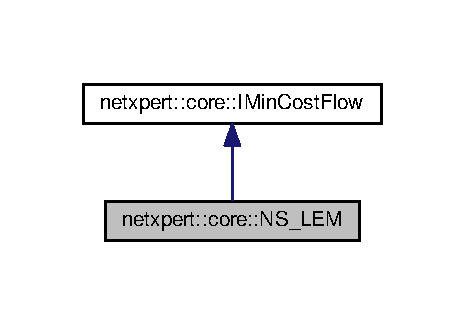
\includegraphics[width=223pt]{classnetxpert_1_1core_1_1NS__LEM__inherit__graph}
\end{center}
\end{figure}


Collaboration diagram for netxpert\+:\+:core\+:\+:N\+S\+\_\+\+L\+EM\+:\nopagebreak
\begin{figure}[H]
\begin{center}
\leavevmode
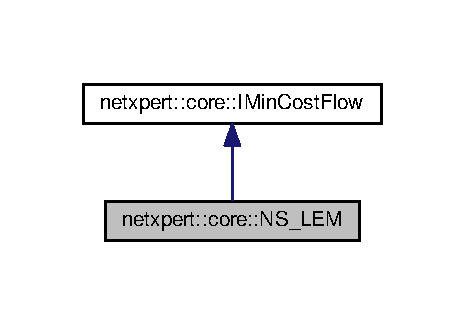
\includegraphics[width=223pt]{classnetxpert_1_1core_1_1NS__LEM__coll__graph}
\end{center}
\end{figure}
\subsection*{Public Member Functions}
\begin{DoxyCompactItemize}
\item 
void {\bfseries Load\+Net} (const uint32\+\_\+t nmax, const uint32\+\_\+t mmax, lemon\+::\+Filter\+Arcs$<$ netxpert\+::data\+::graph\+\_\+t, netxpert\+::data\+::graph\+\_\+t\+::\+Arc\+Map$<$ bool $>$$>$ $\ast$sg, netxpert\+::data\+::graph\+\_\+t\+::\+Arc\+Map$<$ netxpert\+::data\+::cost\+\_\+t $>$ $\ast$\+\_\+cost\+Map, netxpert\+::data\+::graph\+\_\+t\+::\+Arc\+Map$<$ netxpert\+::data\+::capacity\+\_\+t $>$ $\ast$\+\_\+cap\+Map, netxpert\+::data\+::graph\+\_\+t\+::\+Node\+Map$<$ supply\+\_\+t $>$ $\ast$\+\_\+supply\+Map)\hypertarget{classnetxpert_1_1core_1_1NS__LEM_a5cdf7a28a16732ce28eb95fe3255db2a}{}\label{classnetxpert_1_1core_1_1NS__LEM_a5cdf7a28a16732ce28eb95fe3255db2a}

\item 
const uint32\+\_\+t {\bfseries Get\+Arc\+Count} ()\hypertarget{classnetxpert_1_1core_1_1NS__LEM_a03a501e91d92869badc51835059a63d9}{}\label{classnetxpert_1_1core_1_1NS__LEM_a03a501e91d92869badc51835059a63d9}

\item 
const uint32\+\_\+t {\bfseries Get\+Node\+Count} ()\hypertarget{classnetxpert_1_1core_1_1NS__LEM_aec06454662c27708f592a7b4dc3f3c93}{}\label{classnetxpert_1_1core_1_1NS__LEM_aec06454662c27708f592a7b4dc3f3c93}

\item 
void {\bfseries Solve\+M\+CF} ()\hypertarget{classnetxpert_1_1core_1_1NS__LEM_ae34d52960b82c712554362e7730103c0}{}\label{classnetxpert_1_1core_1_1NS__LEM_ae34d52960b82c712554362e7730103c0}

\item 
const double {\bfseries Get\+Optimum} () const \hypertarget{classnetxpert_1_1core_1_1NS__LEM_a1458d55ff84f74ad2fbe040033bee38c}{}\label{classnetxpert_1_1core_1_1NS__LEM_a1458d55ff84f74ad2fbe040033bee38c}

\item 
std\+::vector$<$ netxpert\+::data\+::arc\+\_\+t $>$ {\bfseries Get\+M\+C\+F\+Arcs} ()\hypertarget{classnetxpert_1_1core_1_1NS__LEM_ad12184f360951418f2e00e3bfa0fe746}{}\label{classnetxpert_1_1core_1_1NS__LEM_ad12184f360951418f2e00e3bfa0fe746}

\item 
netxpert\+::data\+::graph\+\_\+t\+::\+Arc\+Map$<$ netxpert\+::data\+::flow\+\_\+t $>$ $\ast$ {\bfseries Get\+M\+C\+F\+Flow} ()\hypertarget{classnetxpert_1_1core_1_1NS__LEM_ae7cb3ce93684294d2f87c2504aa9757a}{}\label{classnetxpert_1_1core_1_1NS__LEM_ae7cb3ce93684294d2f87c2504aa9757a}

\item 
netxpert\+::data\+::graph\+\_\+t\+::\+Arc\+Map$<$ netxpert\+::data\+::cost\+\_\+t $>$ $\ast$ {\bfseries Get\+M\+C\+F\+Cost} ()\hypertarget{classnetxpert_1_1core_1_1NS__LEM_aa93b64efcb6242a9222d6ecb0146eef8}{}\label{classnetxpert_1_1core_1_1NS__LEM_aa93b64efcb6242a9222d6ecb0146eef8}

\item 
const int {\bfseries Get\+M\+C\+F\+Status} ()\hypertarget{classnetxpert_1_1core_1_1NS__LEM_ad94b6da1ebbf367b903f178ea6f8df01}{}\label{classnetxpert_1_1core_1_1NS__LEM_ad94b6da1ebbf367b903f178ea6f8df01}

\item 
void {\bfseries Print\+Result} ()\hypertarget{classnetxpert_1_1core_1_1NS__LEM_abf5de9e17e749ff12935439a833968da}{}\label{classnetxpert_1_1core_1_1NS__LEM_abf5de9e17e749ff12935439a833968da}

\end{DoxyCompactItemize}
\subsection*{Protected Attributes}
\begin{DoxyCompactItemize}
\item 
uint32\+\_\+t {\bfseries nmax}\hypertarget{classnetxpert_1_1core_1_1NS__LEM_a7d9ac4a6d045532e29d4485d2a3e2c87}{}\label{classnetxpert_1_1core_1_1NS__LEM_a7d9ac4a6d045532e29d4485d2a3e2c87}

\item 
uint32\+\_\+t {\bfseries mmax}\hypertarget{classnetxpert_1_1core_1_1NS__LEM_a1782bde4d1fbcef5ce6ce937cebc9d0e}{}\label{classnetxpert_1_1core_1_1NS__LEM_a1782bde4d1fbcef5ce6ce937cebc9d0e}

\end{DoxyCompactItemize}


\subsection{Detailed Description}
Core Solver for the Minimum Cost Flow Problem with the Network Simplex algorithm of L\+E\+M\+ON. 

The documentation for this class was generated from the following file\+:\begin{DoxyCompactItemize}
\item 
/home/hahne/dev/netxpert1\+\_\+0/include/core/nslem.\+h\end{DoxyCompactItemize}

\hypertarget{structnetxpert_1_1data_1_1ODPair}{}\section{netxpert\+:\+:data\+:\+:O\+D\+Pair Struct Reference}
\label{structnetxpert_1_1data_1_1ODPair}\index{netxpert\+::data\+::\+O\+D\+Pair@{netxpert\+::data\+::\+O\+D\+Pair}}


Custom data type for storing lemon \hyperlink{structnetxpert_1_1data_1_1ODPair}{O\+D\+Pair} tuple $<$origin,dest$>$  




{\ttfamily \#include $<$data.\+h$>$}

\subsection*{Public Member Functions}
\begin{DoxyCompactItemize}
\item 
bool {\bfseries operator==} (const \hyperlink{structnetxpert_1_1data_1_1ODPair}{O\+D\+Pair} \&p2) const \hypertarget{structnetxpert_1_1data_1_1ODPair_a4d240c740c3710d9529e714df658ae53}{}\label{structnetxpert_1_1data_1_1ODPair_a4d240c740c3710d9529e714df658ae53}

\item 
bool {\bfseries operator$<$} (const \hyperlink{structnetxpert_1_1data_1_1ODPair}{O\+D\+Pair} \&p2) const \hypertarget{structnetxpert_1_1data_1_1ODPair_afd53307442216ae9a1b1cb5359a107a7}{}\label{structnetxpert_1_1data_1_1ODPair_afd53307442216ae9a1b1cb5359a107a7}

\end{DoxyCompactItemize}
\subsection*{Public Attributes}
\begin{DoxyCompactItemize}
\item 
netxpert\+::data\+::node\+\_\+t {\bfseries origin}\hypertarget{structnetxpert_1_1data_1_1ODPair_a557a8b00799f18a5df315e15f0f8ccb9}{}\label{structnetxpert_1_1data_1_1ODPair_a557a8b00799f18a5df315e15f0f8ccb9}

\item 
netxpert\+::data\+::node\+\_\+t {\bfseries dest}\hypertarget{structnetxpert_1_1data_1_1ODPair_aa1674cccee6cf54f23192cd290ce22a1}{}\label{structnetxpert_1_1data_1_1ODPair_aa1674cccee6cf54f23192cd290ce22a1}

\end{DoxyCompactItemize}


\subsection{Detailed Description}
Custom data type for storing lemon \hyperlink{structnetxpert_1_1data_1_1ODPair}{O\+D\+Pair} tuple $<$origin,dest$>$ 

The documentation for this struct was generated from the following file\+:\begin{DoxyCompactItemize}
\item 
/home/hahne/dev/netxpert1\+\_\+0/include/data.\+h\end{DoxyCompactItemize}

\hypertarget{classnetxpert_1_1OriginDestinationMatrix}{}\section{netxpert\+:\+:Origin\+Destination\+Matrix Class Reference}
\label{classnetxpert_1_1OriginDestinationMatrix}\index{netxpert\+::\+Origin\+Destination\+Matrix@{netxpert\+::\+Origin\+Destination\+Matrix}}


Solver for computing an Origin Destination Matrix.  




{\ttfamily \#include $<$odmatrix.\+h$>$}



Inheritance diagram for netxpert\+:\+:Origin\+Destination\+Matrix\+:\nopagebreak
\begin{figure}[H]
\begin{center}
\leavevmode
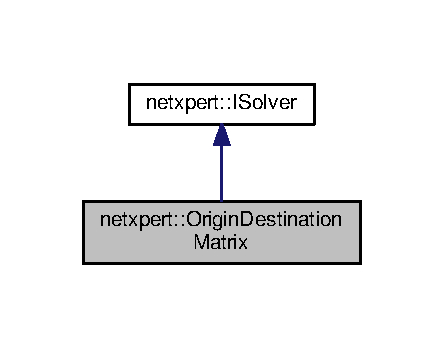
\includegraphics[width=213pt]{classnetxpert_1_1OriginDestinationMatrix__inherit__graph}
\end{center}
\end{figure}


Collaboration diagram for netxpert\+:\+:Origin\+Destination\+Matrix\+:\nopagebreak
\begin{figure}[H]
\begin{center}
\leavevmode
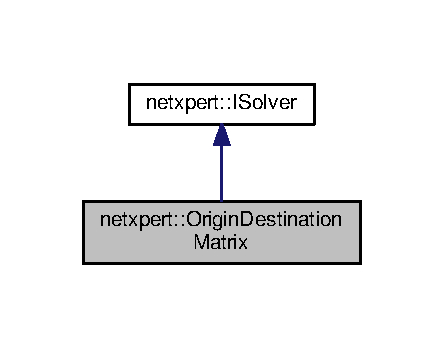
\includegraphics[width=213pt]{classnetxpert_1_1OriginDestinationMatrix__coll__graph}
\end{center}
\end{figure}
\subsection*{Public Member Functions}
\begin{DoxyCompactItemize}
\item 
\hyperlink{classnetxpert_1_1OriginDestinationMatrix_a2ffcb9a8e1698ac09145d5ab08cfb8f4}{Origin\+Destination\+Matrix} (\hyperlink{structnetxpert_1_1cnfg_1_1Config}{netxpert\+::cnfg\+::\+Config} \&cnfg)
\item 
\hyperlink{classnetxpert_1_1OriginDestinationMatrix_ae2337bd32fe54db9027a0ae5612bf247}{$\sim$\+Origin\+Destination\+Matrix} ()
\item 
void {\bfseries Solve} (std\+::string net)\hypertarget{classnetxpert_1_1OriginDestinationMatrix_a6021a419ef2db34a079e508b79b94656}{}\label{classnetxpert_1_1OriginDestinationMatrix_a6021a419ef2db34a079e508b79b94656}

\item 
void {\bfseries Solve} (\hyperlink{classnetxpert_1_1InternalNet}{netxpert\+::\+Internal\+Net} \&net)\hypertarget{classnetxpert_1_1OriginDestinationMatrix_a78f9ae34b0a3caa0711fd4806ce2cad7}{}\label{classnetxpert_1_1OriginDestinationMatrix_a78f9ae34b0a3caa0711fd4806ce2cad7}

\item 
\hyperlink{namespacenetxpert_1_1cnfg_a6ff755ed7f76e0049e3eeeed86c9b55d}{netxpert\+::cnfg\+::\+S\+P\+T\+Algorithm} {\bfseries Get\+Algorithm} () const \hypertarget{classnetxpert_1_1OriginDestinationMatrix_a1ce368d57c55f63a8a3d8a956246f51c}{}\label{classnetxpert_1_1OriginDestinationMatrix_a1ce368d57c55f63a8a3d8a956246f51c}

\item 
void {\bfseries Set\+Algorithm} (\hyperlink{namespacenetxpert_1_1cnfg_a6ff755ed7f76e0049e3eeeed86c9b55d}{netxpert\+::cnfg\+::\+S\+P\+T\+Algorithm} mst\+Algorithm)\hypertarget{classnetxpert_1_1OriginDestinationMatrix_a97634a566c9cb0f4d16f09460695dca5}{}\label{classnetxpert_1_1OriginDestinationMatrix_a97634a566c9cb0f4d16f09460695dca5}

\item 
int {\bfseries Get\+S\+P\+T\+Heap\+Card} () const \hypertarget{classnetxpert_1_1OriginDestinationMatrix_a9a74ba346eb886f6364cf8ee49fc999b}{}\label{classnetxpert_1_1OriginDestinationMatrix_a9a74ba346eb886f6364cf8ee49fc999b}

\item 
void {\bfseries Set\+S\+P\+T\+Heap\+Card} (int heap\+Card)\hypertarget{classnetxpert_1_1OriginDestinationMatrix_a3eccac28a93415efcde47fb7c5864513}{}\label{classnetxpert_1_1OriginDestinationMatrix_a3eccac28a93415efcde47fb7c5864513}

\item 
\hyperlink{namespacenetxpert_1_1cnfg_a1514d3ae51414bf0bcd8d1fe8e868b89}{netxpert\+::cnfg\+::\+G\+E\+O\+M\+E\+T\+R\+Y\+\_\+\+H\+A\+N\+D\+L\+I\+NG} {\bfseries Get\+Geometry\+Handling} () const \hypertarget{classnetxpert_1_1OriginDestinationMatrix_a4c13924e741f428b858126b4cee8fc5c}{}\label{classnetxpert_1_1OriginDestinationMatrix_a4c13924e741f428b858126b4cee8fc5c}

\item 
void {\bfseries Set\+Geometry\+Handling} (\hyperlink{namespacenetxpert_1_1cnfg_a1514d3ae51414bf0bcd8d1fe8e868b89}{netxpert\+::cnfg\+::\+G\+E\+O\+M\+E\+T\+R\+Y\+\_\+\+H\+A\+N\+D\+L\+I\+NG} geom\+Handling)\hypertarget{classnetxpert_1_1OriginDestinationMatrix_a429a93b66e57d7a1c1a4d621b4676162}{}\label{classnetxpert_1_1OriginDestinationMatrix_a429a93b66e57d7a1c1a4d621b4676162}

\item 
void {\bfseries Set\+Origins} (std\+::vector$<$ netxpert\+::data\+::node\+\_\+t $>$ \&origs)\hypertarget{classnetxpert_1_1OriginDestinationMatrix_ae799703ff303d31e2c26b4bced78ac43}{}\label{classnetxpert_1_1OriginDestinationMatrix_ae799703ff303d31e2c26b4bced78ac43}

\item 
void \hyperlink{classnetxpert_1_1OriginDestinationMatrix_af6235667a08d4fca3b1d88cbb4fec513}{Set\+Origins} (const std\+::vector$<$ uint32\+\_\+t $>$ \&origs)
\item 
void {\bfseries Set\+Origins} (std\+::vector$<$ std\+::pair$<$ netxpert\+::data\+::node\+\_\+t, std\+::string $>$$>$ \&origs)\hypertarget{classnetxpert_1_1OriginDestinationMatrix_a6842884d4c037bfaf21f892c4bc49f39}{}\label{classnetxpert_1_1OriginDestinationMatrix_a6842884d4c037bfaf21f892c4bc49f39}

\item 
std\+::vector$<$ netxpert\+::data\+::node\+\_\+t $>$ {\bfseries Get\+Origins} () const \hypertarget{classnetxpert_1_1OriginDestinationMatrix_a070086cd6c9dfd56c6d647bdb4d1f044}{}\label{classnetxpert_1_1OriginDestinationMatrix_a070086cd6c9dfd56c6d647bdb4d1f044}

\item 
std\+::vector$<$ uint32\+\_\+t $>$ \hyperlink{classnetxpert_1_1OriginDestinationMatrix_ad18ee15d95918031e6e69af7cced7be8}{Get\+Origin\+I\+Ds} () const 
\item 
void {\bfseries Set\+Destinations} (std\+::vector$<$ netxpert\+::data\+::node\+\_\+t $>$ \&dests)\hypertarget{classnetxpert_1_1OriginDestinationMatrix_a85be24fc41f55f43c371e531ea9c3814}{}\label{classnetxpert_1_1OriginDestinationMatrix_a85be24fc41f55f43c371e531ea9c3814}

\item 
void \hyperlink{classnetxpert_1_1OriginDestinationMatrix_ac0ae25a4fd186aeee1ce7c1b50538a62}{Set\+Destinations} (const std\+::vector$<$ uint32\+\_\+t $>$ \&dests)
\item 
void {\bfseries Set\+Destinations} (std\+::vector$<$ std\+::pair$<$ netxpert\+::data\+::node\+\_\+t, std\+::string $>$$>$ \&dests)\hypertarget{classnetxpert_1_1OriginDestinationMatrix_a05b29c743df9d1d9002d682e47c791ba}{}\label{classnetxpert_1_1OriginDestinationMatrix_a05b29c743df9d1d9002d682e47c791ba}

\item 
std\+::vector$<$ netxpert\+::data\+::node\+\_\+t $>$ {\bfseries Get\+Destinations} () const \hypertarget{classnetxpert_1_1OriginDestinationMatrix_aee97b176bc22b67dc3381af2a858be74}{}\label{classnetxpert_1_1OriginDestinationMatrix_aee97b176bc22b67dc3381af2a858be74}

\item 
std\+::vector$<$ uint32\+\_\+t $>$ \hyperlink{classnetxpert_1_1OriginDestinationMatrix_a92652a2389da24d35f6f1233a1298f91}{Get\+Destination\+I\+Ds} () const 
\item 
std\+::vector$<$ netxpert\+::data\+::node\+\_\+t $>$ {\bfseries Get\+Reached\+Dests} () const \hypertarget{classnetxpert_1_1OriginDestinationMatrix_abdcfabcf36cc23240bd13ed0a021704d}{}\label{classnetxpert_1_1OriginDestinationMatrix_abdcfabcf36cc23240bd13ed0a021704d}

\item 
std\+::vector$<$ uint32\+\_\+t $>$ \hyperlink{classnetxpert_1_1OriginDestinationMatrix_ad7850510d0b31ae9b9d80e795be83756}{Get\+Reached\+Dest\+I\+Ds} () const 
\item 
std\+::map$<$ \hyperlink{structnetxpert_1_1data_1_1ODPair}{netxpert\+::data\+::\+O\+D\+Pair}, \hyperlink{namespacenetxpert_1_1data_a82e488b55f222a9759d73e24f6087033}{netxpert\+::data\+::\+Compressed\+Path} $>$ {\bfseries Get\+Shortest\+Paths} () const \hypertarget{classnetxpert_1_1OriginDestinationMatrix_a0685f3a1113698381631ab37b71fa0ba}{}\label{classnetxpert_1_1OriginDestinationMatrix_a0685f3a1113698381631ab37b71fa0ba}

\item 
std\+::map$<$ \hyperlink{structnetxpert_1_1data_1_1ODPair}{netxpert\+::data\+::\+O\+D\+Pair}, netxpert\+::data\+::cost\+\_\+t $>$ {\bfseries Get\+O\+D\+Matrix} () const \hypertarget{classnetxpert_1_1OriginDestinationMatrix_a7fa514c840cda5d6e8c076b15dc807e6}{}\label{classnetxpert_1_1OriginDestinationMatrix_a7fa514c840cda5d6e8c076b15dc807e6}

\item 
const double {\bfseries Get\+Optimum} () const \hypertarget{classnetxpert_1_1OriginDestinationMatrix_a0d02226f1246cc54aca03dbdfddabb62}{}\label{classnetxpert_1_1OriginDestinationMatrix_a0d02226f1246cc54aca03dbdfddabb62}

\item 
void {\bfseries Save\+Results} (const std\+::string \&result\+Table\+Name, const \hyperlink{structnetxpert_1_1data_1_1ColumnMap}{netxpert\+::data\+::\+Column\+Map} \&cmap) const \hypertarget{classnetxpert_1_1OriginDestinationMatrix_a2dccec6e7af7d844d38e9ab3f8f151b9}{}\label{classnetxpert_1_1OriginDestinationMatrix_a2dccec6e7af7d844d38e9ab3f8f151b9}

\end{DoxyCompactItemize}


\subsection{Detailed Description}
Solver for computing an Origin Destination Matrix. 

\subsection{Constructor \& Destructor Documentation}
\index{netxpert\+::\+Origin\+Destination\+Matrix@{netxpert\+::\+Origin\+Destination\+Matrix}!Origin\+Destination\+Matrix@{Origin\+Destination\+Matrix}}
\index{Origin\+Destination\+Matrix@{Origin\+Destination\+Matrix}!netxpert\+::\+Origin\+Destination\+Matrix@{netxpert\+::\+Origin\+Destination\+Matrix}}
\subsubsection[{\texorpdfstring{Origin\+Destination\+Matrix(netxpert\+::cnfg\+::\+Config \&cnfg)}{OriginDestinationMatrix(netxpert::cnfg::Config &cnfg)}}]{\setlength{\rightskip}{0pt plus 5cm}netxpert\+::\+Origin\+Destination\+Matrix\+::\+Origin\+Destination\+Matrix (
\begin{DoxyParamCaption}
\item[{{\bf netxpert\+::cnfg\+::\+Config} \&}]{cnfg}
\end{DoxyParamCaption}
)}\hypertarget{classnetxpert_1_1OriginDestinationMatrix_a2ffcb9a8e1698ac09145d5ab08cfb8f4}{}\label{classnetxpert_1_1OriginDestinationMatrix_a2ffcb9a8e1698ac09145d5ab08cfb8f4}
Default constructor \index{netxpert\+::\+Origin\+Destination\+Matrix@{netxpert\+::\+Origin\+Destination\+Matrix}!````~Origin\+Destination\+Matrix@{$\sim$\+Origin\+Destination\+Matrix}}
\index{````~Origin\+Destination\+Matrix@{$\sim$\+Origin\+Destination\+Matrix}!netxpert\+::\+Origin\+Destination\+Matrix@{netxpert\+::\+Origin\+Destination\+Matrix}}
\subsubsection[{\texorpdfstring{$\sim$\+Origin\+Destination\+Matrix()}{~OriginDestinationMatrix()}}]{\setlength{\rightskip}{0pt plus 5cm}netxpert\+::\+Origin\+Destination\+Matrix\+::$\sim$\+Origin\+Destination\+Matrix (
\begin{DoxyParamCaption}
{}
\end{DoxyParamCaption}
)\hspace{0.3cm}{\ttfamily [inline]}}\hypertarget{classnetxpert_1_1OriginDestinationMatrix_ae2337bd32fe54db9027a0ae5612bf247}{}\label{classnetxpert_1_1OriginDestinationMatrix_ae2337bd32fe54db9027a0ae5612bf247}
Default destructor 

\subsection{Member Function Documentation}
\index{netxpert\+::\+Origin\+Destination\+Matrix@{netxpert\+::\+Origin\+Destination\+Matrix}!Get\+Destination\+I\+Ds@{Get\+Destination\+I\+Ds}}
\index{Get\+Destination\+I\+Ds@{Get\+Destination\+I\+Ds}!netxpert\+::\+Origin\+Destination\+Matrix@{netxpert\+::\+Origin\+Destination\+Matrix}}
\subsubsection[{\texorpdfstring{Get\+Destination\+I\+Ds() const }{GetDestinationIDs() const }}]{\setlength{\rightskip}{0pt plus 5cm}std\+::vector$<$uint32\+\_\+t$>$ netxpert\+::\+Origin\+Destination\+Matrix\+::\+Get\+Destination\+I\+Ds (
\begin{DoxyParamCaption}
{}
\end{DoxyParamCaption}
) const}\hypertarget{classnetxpert_1_1OriginDestinationMatrix_a92652a2389da24d35f6f1233a1298f91}{}\label{classnetxpert_1_1OriginDestinationMatrix_a92652a2389da24d35f6f1233a1298f91}
Simple Wrapper for S\+W\+IG \index{netxpert\+::\+Origin\+Destination\+Matrix@{netxpert\+::\+Origin\+Destination\+Matrix}!Get\+Origin\+I\+Ds@{Get\+Origin\+I\+Ds}}
\index{Get\+Origin\+I\+Ds@{Get\+Origin\+I\+Ds}!netxpert\+::\+Origin\+Destination\+Matrix@{netxpert\+::\+Origin\+Destination\+Matrix}}
\subsubsection[{\texorpdfstring{Get\+Origin\+I\+Ds() const }{GetOriginIDs() const }}]{\setlength{\rightskip}{0pt plus 5cm}std\+::vector$<$uint32\+\_\+t$>$ netxpert\+::\+Origin\+Destination\+Matrix\+::\+Get\+Origin\+I\+Ds (
\begin{DoxyParamCaption}
{}
\end{DoxyParamCaption}
) const\hspace{0.3cm}{\ttfamily [inline]}}\hypertarget{classnetxpert_1_1OriginDestinationMatrix_ad18ee15d95918031e6e69af7cced7be8}{}\label{classnetxpert_1_1OriginDestinationMatrix_ad18ee15d95918031e6e69af7cced7be8}
Simple Wrapper for S\+W\+IG \index{netxpert\+::\+Origin\+Destination\+Matrix@{netxpert\+::\+Origin\+Destination\+Matrix}!Get\+Reached\+Dest\+I\+Ds@{Get\+Reached\+Dest\+I\+Ds}}
\index{Get\+Reached\+Dest\+I\+Ds@{Get\+Reached\+Dest\+I\+Ds}!netxpert\+::\+Origin\+Destination\+Matrix@{netxpert\+::\+Origin\+Destination\+Matrix}}
\subsubsection[{\texorpdfstring{Get\+Reached\+Dest\+I\+Ds() const }{GetReachedDestIDs() const }}]{\setlength{\rightskip}{0pt plus 5cm}std\+::vector$<$uint32\+\_\+t$>$ netxpert\+::\+Origin\+Destination\+Matrix\+::\+Get\+Reached\+Dest\+I\+Ds (
\begin{DoxyParamCaption}
{}
\end{DoxyParamCaption}
) const}\hypertarget{classnetxpert_1_1OriginDestinationMatrix_ad7850510d0b31ae9b9d80e795be83756}{}\label{classnetxpert_1_1OriginDestinationMatrix_ad7850510d0b31ae9b9d80e795be83756}
Simple Wrapper for S\+W\+IG \index{netxpert\+::\+Origin\+Destination\+Matrix@{netxpert\+::\+Origin\+Destination\+Matrix}!Set\+Destinations@{Set\+Destinations}}
\index{Set\+Destinations@{Set\+Destinations}!netxpert\+::\+Origin\+Destination\+Matrix@{netxpert\+::\+Origin\+Destination\+Matrix}}
\subsubsection[{\texorpdfstring{Set\+Destinations(const std\+::vector$<$ uint32\+\_\+t $>$ \&dests)}{SetDestinations(const std::vector< uint32_t > &dests)}}]{\setlength{\rightskip}{0pt plus 5cm}void netxpert\+::\+Origin\+Destination\+Matrix\+::\+Set\+Destinations (
\begin{DoxyParamCaption}
\item[{const std\+::vector$<$ uint32\+\_\+t $>$ \&}]{dests}
\end{DoxyParamCaption}
)\hspace{0.3cm}{\ttfamily [inline]}}\hypertarget{classnetxpert_1_1OriginDestinationMatrix_ac0ae25a4fd186aeee1ce7c1b50538a62}{}\label{classnetxpert_1_1OriginDestinationMatrix_ac0ae25a4fd186aeee1ce7c1b50538a62}
Simple Wrapper for S\+W\+IG \index{netxpert\+::\+Origin\+Destination\+Matrix@{netxpert\+::\+Origin\+Destination\+Matrix}!Set\+Origins@{Set\+Origins}}
\index{Set\+Origins@{Set\+Origins}!netxpert\+::\+Origin\+Destination\+Matrix@{netxpert\+::\+Origin\+Destination\+Matrix}}
\subsubsection[{\texorpdfstring{Set\+Origins(const std\+::vector$<$ uint32\+\_\+t $>$ \&origs)}{SetOrigins(const std::vector< uint32_t > &origs)}}]{\setlength{\rightskip}{0pt plus 5cm}void netxpert\+::\+Origin\+Destination\+Matrix\+::\+Set\+Origins (
\begin{DoxyParamCaption}
\item[{const std\+::vector$<$ uint32\+\_\+t $>$ \&}]{origs}
\end{DoxyParamCaption}
)\hspace{0.3cm}{\ttfamily [inline]}}\hypertarget{classnetxpert_1_1OriginDestinationMatrix_af6235667a08d4fca3b1d88cbb4fec513}{}\label{classnetxpert_1_1OriginDestinationMatrix_af6235667a08d4fca3b1d88cbb4fec513}
Simple Wrapper for S\+W\+IG 

The documentation for this class was generated from the following file\+:\begin{DoxyCompactItemize}
\item 
/home/hahne/dev/netxpert1\+\_\+0/include/solver/odmatrix.\+h\end{DoxyCompactItemize}

\hypertarget{classnetxpert_1_1simple_1_1OriginDestinationMatrix}{}\section{netxpert\+:\+:simple\+:\+:Origin\+Destination\+Matrix Class Reference}
\label{classnetxpert_1_1simple_1_1OriginDestinationMatrix}\index{netxpert\+::simple\+::\+Origin\+Destination\+Matrix@{netxpert\+::simple\+::\+Origin\+Destination\+Matrix}}
\subsection*{Public Member Functions}
\begin{DoxyCompactItemize}
\item 
{\bfseries Origin\+Destination\+Matrix} (std\+::string json\+Cnfg)\hypertarget{classnetxpert_1_1simple_1_1OriginDestinationMatrix_af8c50cacd33cc7e744eba19b236bf0d0}{}\label{classnetxpert_1_1simple_1_1OriginDestinationMatrix_af8c50cacd33cc7e744eba19b236bf0d0}

\item 
int {\bfseries Solve} ()\hypertarget{classnetxpert_1_1simple_1_1OriginDestinationMatrix_a0ae3ad35c6c2ce358634c931f1cd6c7b}{}\label{classnetxpert_1_1simple_1_1OriginDestinationMatrix_a0ae3ad35c6c2ce358634c931f1cd6c7b}

\item 
int {\bfseries Solve} (bool parallel)\hypertarget{classnetxpert_1_1simple_1_1OriginDestinationMatrix_ac746559fd6d2543df7cf0204556413c8}{}\label{classnetxpert_1_1simple_1_1OriginDestinationMatrix_ac746559fd6d2543df7cf0204556413c8}

\item 
double {\bfseries Get\+Optimum} ()\hypertarget{classnetxpert_1_1simple_1_1OriginDestinationMatrix_aa5cfa1d67d46d0f316a3372cee884023}{}\label{classnetxpert_1_1simple_1_1OriginDestinationMatrix_aa5cfa1d67d46d0f316a3372cee884023}

\item 
std\+::string {\bfseries Get\+O\+D\+Matrix\+As\+J\+S\+ON} ()\hypertarget{classnetxpert_1_1simple_1_1OriginDestinationMatrix_a553d23d199377b96c16d21d286809cd8}{}\label{classnetxpert_1_1simple_1_1OriginDestinationMatrix_a553d23d199377b96c16d21d286809cd8}

\item 
std\+::vector$<$ \hyperlink{structnetxpert_1_1data_1_1ExtSPTreeArc}{netxpert\+::data\+::\+Ext\+S\+P\+Tree\+Arc} $>$ {\bfseries Get\+O\+D\+Matrix} ()\hypertarget{classnetxpert_1_1simple_1_1OriginDestinationMatrix_adca164a4061f90ba3d534ae0fda98afb}{}\label{classnetxpert_1_1simple_1_1OriginDestinationMatrix_adca164a4061f90ba3d534ae0fda98afb}

\end{DoxyCompactItemize}


The documentation for this class was generated from the following file\+:\begin{DoxyCompactItemize}
\item 
/home/hahne/dev/netxpert1\+\_\+0/include/simple/odmatrix\+\_\+simple.\+h\end{DoxyCompactItemize}

\hypertarget{classnetxpert_1_1ShortestPathTree}{}\section{netxpert\+:\+:Shortest\+Path\+Tree Class Reference}
\label{classnetxpert_1_1ShortestPathTree}\index{netxpert\+::\+Shortest\+Path\+Tree@{netxpert\+::\+Shortest\+Path\+Tree}}


Solver for the Shortest Path Tree Problem.  




{\ttfamily \#include $<$sptree.\+h$>$}



Inheritance diagram for netxpert\+:\+:Shortest\+Path\+Tree\+:\nopagebreak
\begin{figure}[H]
\begin{center}
\leavevmode
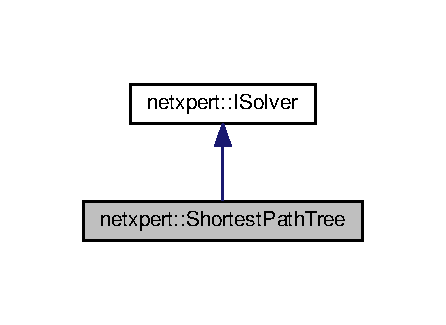
\includegraphics[width=214pt]{classnetxpert_1_1ShortestPathTree__inherit__graph}
\end{center}
\end{figure}


Collaboration diagram for netxpert\+:\+:Shortest\+Path\+Tree\+:\nopagebreak
\begin{figure}[H]
\begin{center}
\leavevmode
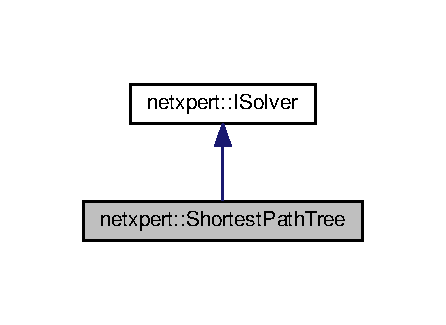
\includegraphics[width=214pt]{classnetxpert_1_1ShortestPathTree__coll__graph}
\end{center}
\end{figure}
\subsection*{Public Member Functions}
\begin{DoxyCompactItemize}
\item 
\hyperlink{classnetxpert_1_1ShortestPathTree_a98b5de4fe83005fdba7216253d81b4f8}{Shortest\+Path\+Tree} (\hyperlink{structnetxpert_1_1cnfg_1_1Config}{netxpert\+::cnfg\+::\+Config} \&cnfg)
\item 
\hyperlink{classnetxpert_1_1ShortestPathTree_a6f1ad2e2a4f8f99927eb960a4c706d34}{$\sim$\+Shortest\+Path\+Tree} ()
\item 
void {\bfseries Solve} (std\+::string net)\hypertarget{classnetxpert_1_1ShortestPathTree_a9d051b476c6e16c8382f00c6fd41443c}{}\label{classnetxpert_1_1ShortestPathTree_a9d051b476c6e16c8382f00c6fd41443c}

\item 
void {\bfseries Solve} (\hyperlink{classnetxpert_1_1InternalNet}{netxpert\+::\+Internal\+Net} \&net)\hypertarget{classnetxpert_1_1ShortestPathTree_afaab6c93fa959a87162b23d65a7e77c6}{}\label{classnetxpert_1_1ShortestPathTree_afaab6c93fa959a87162b23d65a7e77c6}

\item 
\hyperlink{namespacenetxpert_1_1cnfg_a6ff755ed7f76e0049e3eeeed86c9b55d}{netxpert\+::cnfg\+::\+S\+P\+T\+Algorithm} {\bfseries Get\+Algorithm} () const \hypertarget{classnetxpert_1_1ShortestPathTree_a3991a05aedb7e38953aa1031db9566bd}{}\label{classnetxpert_1_1ShortestPathTree_a3991a05aedb7e38953aa1031db9566bd}

\item 
void {\bfseries Set\+Algorithm} (\hyperlink{namespacenetxpert_1_1cnfg_a6ff755ed7f76e0049e3eeeed86c9b55d}{netxpert\+::cnfg\+::\+S\+P\+T\+Algorithm} spt\+Algorithm)\hypertarget{classnetxpert_1_1ShortestPathTree_a25a50385e71110a61f13f7627123f38d}{}\label{classnetxpert_1_1ShortestPathTree_a25a50385e71110a61f13f7627123f38d}

\item 
int {\bfseries Get\+S\+P\+T\+Heap\+Card} () const \hypertarget{classnetxpert_1_1ShortestPathTree_a27ba660aebb8e7542a640ed89af60b63}{}\label{classnetxpert_1_1ShortestPathTree_a27ba660aebb8e7542a640ed89af60b63}

\item 
void {\bfseries Set\+S\+P\+T\+Heap\+Card} (int heap\+Card)\hypertarget{classnetxpert_1_1ShortestPathTree_a7d0f7d46f546d67c4d14f561935f4d45}{}\label{classnetxpert_1_1ShortestPathTree_a7d0f7d46f546d67c4d14f561935f4d45}

\item 
\hyperlink{namespacenetxpert_1_1cnfg_a1514d3ae51414bf0bcd8d1fe8e868b89}{netxpert\+::cnfg\+::\+G\+E\+O\+M\+E\+T\+R\+Y\+\_\+\+H\+A\+N\+D\+L\+I\+NG} {\bfseries Get\+Geometry\+Handling} () const \hypertarget{classnetxpert_1_1ShortestPathTree_aef627a9c761474e1bad3152e29705f21}{}\label{classnetxpert_1_1ShortestPathTree_aef627a9c761474e1bad3152e29705f21}

\item 
void {\bfseries Set\+Geometry\+Handling} (\hyperlink{namespacenetxpert_1_1cnfg_a1514d3ae51414bf0bcd8d1fe8e868b89}{netxpert\+::cnfg\+::\+G\+E\+O\+M\+E\+T\+R\+Y\+\_\+\+H\+A\+N\+D\+L\+I\+NG} geom\+Handling)\hypertarget{classnetxpert_1_1ShortestPathTree_ad87ceadb7166f331e7ae66fe70126ff2}{}\label{classnetxpert_1_1ShortestPathTree_ad87ceadb7166f331e7ae66fe70126ff2}

\item 
const netxpert\+::data\+::node\+\_\+t {\bfseries Get\+Origin} () const \hypertarget{classnetxpert_1_1ShortestPathTree_aa760de850ca158259580031115c5eb08}{}\label{classnetxpert_1_1ShortestPathTree_aa760de850ca158259580031115c5eb08}

\item 
const uint32\+\_\+t \hyperlink{classnetxpert_1_1ShortestPathTree_a2902fa8ea1f028e3db1f30957fe80bb3}{Get\+Origin\+ID} () const 
\item 
void {\bfseries Set\+Origin} (const netxpert\+::data\+::node\+\_\+t orig)\hypertarget{classnetxpert_1_1ShortestPathTree_ab15a0c08e48a18ae0f9005ecc6b06f2e}{}\label{classnetxpert_1_1ShortestPathTree_ab15a0c08e48a18ae0f9005ecc6b06f2e}

\item 
void \hyperlink{classnetxpert_1_1ShortestPathTree_a8cdf595af07fc9a9cfd43519a61616ac}{Set\+Origin} (const uint32\+\_\+t orig)
\item 
std\+::vector$<$ netxpert\+::data\+::node\+\_\+t $>$ {\bfseries Get\+Destinations} () const \hypertarget{classnetxpert_1_1ShortestPathTree_a6f1682d49ced42f47cbc10377b89e8ed}{}\label{classnetxpert_1_1ShortestPathTree_a6f1682d49ced42f47cbc10377b89e8ed}

\item 
std\+::vector$<$ uint32\+\_\+t $>$ \hyperlink{classnetxpert_1_1ShortestPathTree_a0c58dd334c20fc9d9fc54788f5cd009d}{Get\+Destination\+I\+Ds} () const 
\item 
void {\bfseries Set\+Destinations} (const std\+::vector$<$ netxpert\+::data\+::node\+\_\+t $>$ \&dests)\hypertarget{classnetxpert_1_1ShortestPathTree_ade834f898cdb04271bf5a03761da5c29}{}\label{classnetxpert_1_1ShortestPathTree_ade834f898cdb04271bf5a03761da5c29}

\item 
void \hyperlink{classnetxpert_1_1ShortestPathTree_a9fe7e9de16da3589962ddc1e16838691}{Set\+Destinations} (const std\+::vector$<$ uint32\+\_\+t $>$ \&dests)
\item 
std\+::vector$<$ netxpert\+::data\+::node\+\_\+t $>$ {\bfseries Get\+Reached\+Dests} () const \hypertarget{classnetxpert_1_1ShortestPathTree_a5793c2237688107aaedefeeff33af23c}{}\label{classnetxpert_1_1ShortestPathTree_a5793c2237688107aaedefeeff33af23c}

\item 
std\+::vector$<$ uint32\+\_\+t $>$ {\bfseries Get\+Reached\+Dest\+I\+Ds} () const \hypertarget{classnetxpert_1_1ShortestPathTree_ab54e89b59509c274de60ff91fd46d72a}{}\label{classnetxpert_1_1ShortestPathTree_ab54e89b59509c274de60ff91fd46d72a}

\item 
std\+::map$<$ \hyperlink{structnetxpert_1_1data_1_1ODPair}{netxpert\+::data\+::\+O\+D\+Pair}, \hyperlink{namespacenetxpert_1_1data_a82e488b55f222a9759d73e24f6087033}{netxpert\+::data\+::\+Compressed\+Path} $>$ {\bfseries Get\+Shortest\+Paths} () const \hypertarget{classnetxpert_1_1ShortestPathTree_a12d052cbd1d363f93671aae69ac506a6}{}\label{classnetxpert_1_1ShortestPathTree_a12d052cbd1d363f93671aae69ac506a6}

\item 
const double {\bfseries Get\+Optimum} () const \hypertarget{classnetxpert_1_1ShortestPathTree_a3907e625165ffa6492f8815099edc379}{}\label{classnetxpert_1_1ShortestPathTree_a3907e625165ffa6492f8815099edc379}

\item 
void {\bfseries Save\+Results} (const std\+::string \&result\+Table\+Name, const \hyperlink{structnetxpert_1_1data_1_1ColumnMap}{netxpert\+::data\+::\+Column\+Map} \&cmap, const std\+::string \&format=\char`\"{}database\char`\"{}) const \hypertarget{classnetxpert_1_1ShortestPathTree_a5c110d69c62241ad934d50bbf36d8325}{}\label{classnetxpert_1_1ShortestPathTree_a5c110d69c62241ad934d50bbf36d8325}

\end{DoxyCompactItemize}


\subsection{Detailed Description}
Solver for the Shortest Path Tree Problem. 

\subsection{Constructor \& Destructor Documentation}
\index{netxpert\+::\+Shortest\+Path\+Tree@{netxpert\+::\+Shortest\+Path\+Tree}!Shortest\+Path\+Tree@{Shortest\+Path\+Tree}}
\index{Shortest\+Path\+Tree@{Shortest\+Path\+Tree}!netxpert\+::\+Shortest\+Path\+Tree@{netxpert\+::\+Shortest\+Path\+Tree}}
\subsubsection[{\texorpdfstring{Shortest\+Path\+Tree(netxpert\+::cnfg\+::\+Config \&cnfg)}{ShortestPathTree(netxpert::cnfg::Config &cnfg)}}]{\setlength{\rightskip}{0pt plus 5cm}netxpert\+::\+Shortest\+Path\+Tree\+::\+Shortest\+Path\+Tree (
\begin{DoxyParamCaption}
\item[{{\bf netxpert\+::cnfg\+::\+Config} \&}]{cnfg}
\end{DoxyParamCaption}
)}\hypertarget{classnetxpert_1_1ShortestPathTree_a98b5de4fe83005fdba7216253d81b4f8}{}\label{classnetxpert_1_1ShortestPathTree_a98b5de4fe83005fdba7216253d81b4f8}
Default constructor \index{netxpert\+::\+Shortest\+Path\+Tree@{netxpert\+::\+Shortest\+Path\+Tree}!````~Shortest\+Path\+Tree@{$\sim$\+Shortest\+Path\+Tree}}
\index{````~Shortest\+Path\+Tree@{$\sim$\+Shortest\+Path\+Tree}!netxpert\+::\+Shortest\+Path\+Tree@{netxpert\+::\+Shortest\+Path\+Tree}}
\subsubsection[{\texorpdfstring{$\sim$\+Shortest\+Path\+Tree()}{~ShortestPathTree()}}]{\setlength{\rightskip}{0pt plus 5cm}netxpert\+::\+Shortest\+Path\+Tree\+::$\sim$\+Shortest\+Path\+Tree (
\begin{DoxyParamCaption}
{}
\end{DoxyParamCaption}
)\hspace{0.3cm}{\ttfamily [inline]}}\hypertarget{classnetxpert_1_1ShortestPathTree_a6f1ad2e2a4f8f99927eb960a4c706d34}{}\label{classnetxpert_1_1ShortestPathTree_a6f1ad2e2a4f8f99927eb960a4c706d34}
Default destructor 

\subsection{Member Function Documentation}
\index{netxpert\+::\+Shortest\+Path\+Tree@{netxpert\+::\+Shortest\+Path\+Tree}!Get\+Destination\+I\+Ds@{Get\+Destination\+I\+Ds}}
\index{Get\+Destination\+I\+Ds@{Get\+Destination\+I\+Ds}!netxpert\+::\+Shortest\+Path\+Tree@{netxpert\+::\+Shortest\+Path\+Tree}}
\subsubsection[{\texorpdfstring{Get\+Destination\+I\+Ds() const }{GetDestinationIDs() const }}]{\setlength{\rightskip}{0pt plus 5cm}std\+::vector$<$uint32\+\_\+t$>$ netxpert\+::\+Shortest\+Path\+Tree\+::\+Get\+Destination\+I\+Ds (
\begin{DoxyParamCaption}
{}
\end{DoxyParamCaption}
) const}\hypertarget{classnetxpert_1_1ShortestPathTree_a0c58dd334c20fc9d9fc54788f5cd009d}{}\label{classnetxpert_1_1ShortestPathTree_a0c58dd334c20fc9d9fc54788f5cd009d}
Simple Wrapper for S\+W\+IG \index{netxpert\+::\+Shortest\+Path\+Tree@{netxpert\+::\+Shortest\+Path\+Tree}!Get\+Origin\+ID@{Get\+Origin\+ID}}
\index{Get\+Origin\+ID@{Get\+Origin\+ID}!netxpert\+::\+Shortest\+Path\+Tree@{netxpert\+::\+Shortest\+Path\+Tree}}
\subsubsection[{\texorpdfstring{Get\+Origin\+I\+D() const }{GetOriginID() const }}]{\setlength{\rightskip}{0pt plus 5cm}const uint32\+\_\+t netxpert\+::\+Shortest\+Path\+Tree\+::\+Get\+Origin\+ID (
\begin{DoxyParamCaption}
{}
\end{DoxyParamCaption}
) const\hspace{0.3cm}{\ttfamily [inline]}}\hypertarget{classnetxpert_1_1ShortestPathTree_a2902fa8ea1f028e3db1f30957fe80bb3}{}\label{classnetxpert_1_1ShortestPathTree_a2902fa8ea1f028e3db1f30957fe80bb3}
Simple Wrapper for S\+W\+IG \index{netxpert\+::\+Shortest\+Path\+Tree@{netxpert\+::\+Shortest\+Path\+Tree}!Set\+Destinations@{Set\+Destinations}}
\index{Set\+Destinations@{Set\+Destinations}!netxpert\+::\+Shortest\+Path\+Tree@{netxpert\+::\+Shortest\+Path\+Tree}}
\subsubsection[{\texorpdfstring{Set\+Destinations(const std\+::vector$<$ uint32\+\_\+t $>$ \&dests)}{SetDestinations(const std::vector< uint32_t > &dests)}}]{\setlength{\rightskip}{0pt plus 5cm}void netxpert\+::\+Shortest\+Path\+Tree\+::\+Set\+Destinations (
\begin{DoxyParamCaption}
\item[{const std\+::vector$<$ uint32\+\_\+t $>$ \&}]{dests}
\end{DoxyParamCaption}
)}\hypertarget{classnetxpert_1_1ShortestPathTree_a9fe7e9de16da3589962ddc1e16838691}{}\label{classnetxpert_1_1ShortestPathTree_a9fe7e9de16da3589962ddc1e16838691}
Simple Wrapper for S\+W\+IG \index{netxpert\+::\+Shortest\+Path\+Tree@{netxpert\+::\+Shortest\+Path\+Tree}!Set\+Origin@{Set\+Origin}}
\index{Set\+Origin@{Set\+Origin}!netxpert\+::\+Shortest\+Path\+Tree@{netxpert\+::\+Shortest\+Path\+Tree}}
\subsubsection[{\texorpdfstring{Set\+Origin(const uint32\+\_\+t orig)}{SetOrigin(const uint32_t orig)}}]{\setlength{\rightskip}{0pt plus 5cm}void netxpert\+::\+Shortest\+Path\+Tree\+::\+Set\+Origin (
\begin{DoxyParamCaption}
\item[{const uint32\+\_\+t}]{orig}
\end{DoxyParamCaption}
)\hspace{0.3cm}{\ttfamily [inline]}}\hypertarget{classnetxpert_1_1ShortestPathTree_a8cdf595af07fc9a9cfd43519a61616ac}{}\label{classnetxpert_1_1ShortestPathTree_a8cdf595af07fc9a9cfd43519a61616ac}
Simple Wrapper for S\+W\+IG 

The documentation for this class was generated from the following file\+:\begin{DoxyCompactItemize}
\item 
/home/hahne/dev/netxpert1\+\_\+0/include/solver/sptree.\+h\end{DoxyCompactItemize}

\hypertarget{classnetxpert_1_1simple_1_1ShortestPathTree}{}\section{netxpert\+:\+:simple\+:\+:Shortest\+Path\+Tree Class Reference}
\label{classnetxpert_1_1simple_1_1ShortestPathTree}\index{netxpert\+::simple\+::\+Shortest\+Path\+Tree@{netxpert\+::simple\+::\+Shortest\+Path\+Tree}}
\subsection*{Public Member Functions}
\begin{DoxyCompactItemize}
\item 
{\bfseries Shortest\+Path\+Tree} (std\+::string json\+Cnfg)\hypertarget{classnetxpert_1_1simple_1_1ShortestPathTree_a4ded1db3e88023be3da94f4817d1264d}{}\label{classnetxpert_1_1simple_1_1ShortestPathTree_a4ded1db3e88023be3da94f4817d1264d}

\item 
int {\bfseries Solve} ()\hypertarget{classnetxpert_1_1simple_1_1ShortestPathTree_a9c144586bb5ddc94c8618437c84027e3}{}\label{classnetxpert_1_1simple_1_1ShortestPathTree_a9c144586bb5ddc94c8618437c84027e3}

\item 
const double {\bfseries Get\+Optimum} () const \hypertarget{classnetxpert_1_1simple_1_1ShortestPathTree_ac0c22005112bf82fecb495d697e86df9}{}\label{classnetxpert_1_1simple_1_1ShortestPathTree_ac0c22005112bf82fecb495d697e86df9}

\item 
std\+::string {\bfseries Get\+Shortest\+Paths\+As\+J\+S\+ON} ()\hypertarget{classnetxpert_1_1simple_1_1ShortestPathTree_a06b7a717cb1efdb6901550a08d2ed7a5}{}\label{classnetxpert_1_1simple_1_1ShortestPathTree_a06b7a717cb1efdb6901550a08d2ed7a5}

\item 
std\+::vector$<$ \hyperlink{structnetxpert_1_1data_1_1ExtSPTreeArc}{netxpert\+::data\+::\+Ext\+S\+P\+Tree\+Arc} $>$ {\bfseries Get\+Shortest\+Paths} ()\hypertarget{classnetxpert_1_1simple_1_1ShortestPathTree_ae6891d22b808390a81aeafbc74fa1235}{}\label{classnetxpert_1_1simple_1_1ShortestPathTree_ae6891d22b808390a81aeafbc74fa1235}

\end{DoxyCompactItemize}


The documentation for this class was generated from the following file\+:\begin{DoxyCompactItemize}
\item 
/home/hahne/dev/netxpert1\+\_\+0/include/simple/sptree\+\_\+simple.\+h\end{DoxyCompactItemize}

\hypertarget{classnetxpert_1_1io_1_1SpatiaLiteWriter}{}\section{netxpert\+:\+:io\+:\+:Spatia\+Lite\+Writer Class Reference}
\label{classnetxpert_1_1io_1_1SpatiaLiteWriter}\index{netxpert\+::io\+::\+Spatia\+Lite\+Writer@{netxpert\+::io\+::\+Spatia\+Lite\+Writer}}


Writes the result of Net\+Xpert into a Spatia\+Lite DB.  




{\ttfamily \#include $<$slitewriter.\+h$>$}



Inheritance diagram for netxpert\+:\+:io\+:\+:Spatia\+Lite\+Writer\+:\nopagebreak
\begin{figure}[H]
\begin{center}
\leavevmode
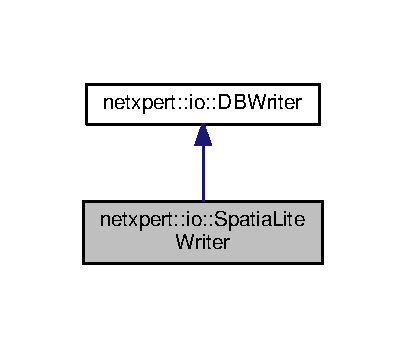
\includegraphics[width=195pt]{classnetxpert_1_1io_1_1SpatiaLiteWriter__inherit__graph}
\end{center}
\end{figure}


Collaboration diagram for netxpert\+:\+:io\+:\+:Spatia\+Lite\+Writer\+:\nopagebreak
\begin{figure}[H]
\begin{center}
\leavevmode
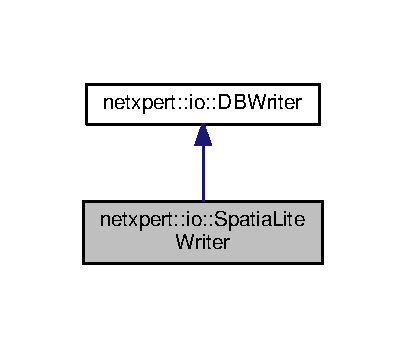
\includegraphics[width=195pt]{classnetxpert_1_1io_1_1SpatiaLiteWriter__coll__graph}
\end{center}
\end{figure}
\subsection*{Public Member Functions}
\begin{DoxyCompactItemize}
\item 
{\bfseries Spatia\+Lite\+Writer} (\hyperlink{structnetxpert_1_1cnfg_1_1Config}{netxpert\+::cnfg\+::\+Config} \&cnfg)\hypertarget{classnetxpert_1_1io_1_1SpatiaLiteWriter_a48bbbeae8faa48aa23691c0651ffd6e1}{}\label{classnetxpert_1_1io_1_1SpatiaLiteWriter_a48bbbeae8faa48aa23691c0651ffd6e1}

\item 
{\bfseries Spatia\+Lite\+Writer} (\hyperlink{structnetxpert_1_1cnfg_1_1Config}{netxpert\+::cnfg\+::\+Config} \&cnfg, std\+::string db\+Path)\hypertarget{classnetxpert_1_1io_1_1SpatiaLiteWriter_af56b5642da873797a7f0455e9c8e7d0a}{}\label{classnetxpert_1_1io_1_1SpatiaLiteWriter_af56b5642da873797a7f0455e9c8e7d0a}

\item 
void {\bfseries Commit\+Current\+Transaction} ()\hypertarget{classnetxpert_1_1io_1_1SpatiaLiteWriter_a760b619e9bf1f1686c7a477fc727c2c2}{}\label{classnetxpert_1_1io_1_1SpatiaLiteWriter_a760b619e9bf1f1686c7a477fc727c2c2}

\item 
void {\bfseries Create\+Net\+Xpert\+DB} ()\hypertarget{classnetxpert_1_1io_1_1SpatiaLiteWriter_aa5aed60ecc92a8aa169cc5f49e73840d}{}\label{classnetxpert_1_1io_1_1SpatiaLiteWriter_aa5aed60ecc92a8aa169cc5f49e73840d}

\item 
void {\bfseries Create\+Solver\+Result\+Table} (const std\+::string \&\+\_\+table\+Name, const \hyperlink{namespacenetxpert_1_1data_a923ee7cb7eab8b9dbfd62fb6d26f51cb}{netxpert\+::data\+::\+Net\+Xpert\+Solver} solver\+Type)\hypertarget{classnetxpert_1_1io_1_1SpatiaLiteWriter_ac98e76bdc1dc0796f20f5a82b548aa93}{}\label{classnetxpert_1_1io_1_1SpatiaLiteWriter_ac98e76bdc1dc0796f20f5a82b548aa93}

\item 
void {\bfseries Create\+Solver\+Result\+Table} (const std\+::string \&\+\_\+table\+Name, const \hyperlink{namespacenetxpert_1_1data_a923ee7cb7eab8b9dbfd62fb6d26f51cb}{netxpert\+::data\+::\+Net\+Xpert\+Solver} solver\+Type, const bool drop\+First)\hypertarget{classnetxpert_1_1io_1_1SpatiaLiteWriter_aac0ed9fe0552f78afab69e8f4cb600c0}{}\label{classnetxpert_1_1io_1_1SpatiaLiteWriter_aac0ed9fe0552f78afab69e8f4cb600c0}

\item 
void {\bfseries Open\+New\+Transaction} ()\hypertarget{classnetxpert_1_1io_1_1SpatiaLiteWriter_aa469d8a214f7a3e2fbbde78480f1ceae}{}\label{classnetxpert_1_1io_1_1SpatiaLiteWriter_aa469d8a214f7a3e2fbbde78480f1ceae}

\item 
std\+::unique\+\_\+ptr$<$ S\+Q\+Lite\+::\+Statement $>$ {\bfseries Prepare\+Save\+Result\+Arc} (const std\+::string \&\+\_\+table\+Name, const \hyperlink{namespacenetxpert_1_1data_a923ee7cb7eab8b9dbfd62fb6d26f51cb}{netxpert\+::data\+::\+Net\+Xpert\+Solver} solver\+Type)\hypertarget{classnetxpert_1_1io_1_1SpatiaLiteWriter_ad2805936f5c7a5791f0f9d37e340abc7}{}\label{classnetxpert_1_1io_1_1SpatiaLiteWriter_ad2805936f5c7a5791f0f9d37e340abc7}

\item 
void \hyperlink{classnetxpert_1_1io_1_1SpatiaLiteWriter_a54a18cc63018ff0e7a8f96248fcf2785}{Save\+Result\+Arc} (const std\+::string \&orig, const std\+::string \&dest, const double cost, const double capacity, const double flow, const geos\+::geom\+::\+Multi\+Line\+String \&route, const std\+::string \&\+\_\+table\+Name, S\+Q\+Lite\+::\+Statement \&query)
\item 
void {\bfseries Save\+Result\+Arc} (const std\+::string \&orig, const std\+::string \&dest, const double cost, const geos\+::geom\+::\+Multi\+Line\+String \&route, const std\+::string \&\+\_\+table\+Name, S\+Q\+Lite\+::\+Statement \&query)\hypertarget{classnetxpert_1_1io_1_1SpatiaLiteWriter_a2095cd746371906d7c890452ae9f7f9f}{}\label{classnetxpert_1_1io_1_1SpatiaLiteWriter_a2095cd746371906d7c890452ae9f7f9f}

\item 
void {\bfseries Save\+Result\+Arc} (const std\+::string \&orig, const double cost, const double cutoff, const geos\+::geom\+::\+Multi\+Line\+String \&route, const std\+::string \&\+\_\+table\+Name, S\+Q\+Lite\+::\+Statement \&query)\hypertarget{classnetxpert_1_1io_1_1SpatiaLiteWriter_ae9a68d34b908fadcfc86487c6012c678}{}\label{classnetxpert_1_1io_1_1SpatiaLiteWriter_ae9a68d34b908fadcfc86487c6012c678}

\item 
void {\bfseries Save\+Result\+Arc} (const std\+::string \&ext\+Arc\+ID, const double cost, const geos\+::geom\+::\+Multi\+Line\+String \&route, const std\+::string \&\+\_\+table\+Name, S\+Q\+Lite\+::\+Statement \&query)\hypertarget{classnetxpert_1_1io_1_1SpatiaLiteWriter_ad5699d9fcd9c30023aa0be395ec004ef}{}\label{classnetxpert_1_1io_1_1SpatiaLiteWriter_ad5699d9fcd9c30023aa0be395ec004ef}

\item 
void \hyperlink{classnetxpert_1_1io_1_1SpatiaLiteWriter_afad833dd75ce96d72718fe8cdac0ba11}{Save\+Network\+Builder\+Arc} (const std\+::string \&ext\+Arc\+ID, const uint32\+\_\+t from\+Node, const uint32\+\_\+t to\+Node, const double cost, const double capacity, const std\+::string \&oneway, const geos\+::geom\+::\+Geometry \&arc, const std\+::string \&\+\_\+table\+Name, S\+Q\+Lite\+::\+Statement \&query)
\item 
std\+::unique\+\_\+ptr$<$ S\+Q\+Lite\+::\+Statement $>$ {\bfseries Prepare\+Merge\+And\+Save\+Result\+Arcs} (std\+::string arc\+Table\+Name)\hypertarget{classnetxpert_1_1io_1_1SpatiaLiteWriter_a1736b92804e3fe4fd7ef15d32f559c47}{}\label{classnetxpert_1_1io_1_1SpatiaLiteWriter_a1736b92804e3fe4fd7ef15d32f559c47}

\item 
void \hyperlink{classnetxpert_1_1io_1_1SpatiaLiteWriter_adeb9fd254a0dbbb576047fbae8475044}{Merge\+And\+Save\+Result\+Arcs} (const std\+::string \&cost\+Column\+Name, const std\+::string \&geom\+Column\+Name, const std\+::string arc\+I\+D\+Column\+Name, const std\+::string \&arc\+Table\+Name, const std\+::string \&arc\+I\+Ds, const std\+::string \&result\+Table\+Name)
\item 
void \hyperlink{classnetxpert_1_1io_1_1SpatiaLiteWriter_a66c389507a4c5d979431c1a6e57e76f5}{Merge\+And\+Save\+Result\+Arcs} (const std\+::string \&orig, const std\+::string \&dest, const double cost, const double capacity, const double flow, const std\+::string \&geom\+Column\+Name, const std\+::string \&arc\+I\+D\+Column\+Name, const std\+::string \&arc\+Table\+Name, const std\+::string \&arc\+I\+Ds, const geos\+::geom\+::\+Multi\+Line\+String \&m\+Line, const std\+::string \&result\+Table\+Name)
\item 
void {\bfseries Close\+Connection} ()\hypertarget{classnetxpert_1_1io_1_1SpatiaLiteWriter_a0785a12e98c75749df06d3b33b98afb9}{}\label{classnetxpert_1_1io_1_1SpatiaLiteWriter_a0785a12e98c75749df06d3b33b98afb9}

\end{DoxyCompactItemize}


\subsection{Detailed Description}
Writes the result of Net\+Xpert into a Spatia\+Lite DB. 

\subsection{Member Function Documentation}
\index{netxpert\+::io\+::\+Spatia\+Lite\+Writer@{netxpert\+::io\+::\+Spatia\+Lite\+Writer}!Merge\+And\+Save\+Result\+Arcs@{Merge\+And\+Save\+Result\+Arcs}}
\index{Merge\+And\+Save\+Result\+Arcs@{Merge\+And\+Save\+Result\+Arcs}!netxpert\+::io\+::\+Spatia\+Lite\+Writer@{netxpert\+::io\+::\+Spatia\+Lite\+Writer}}
\subsubsection[{\texorpdfstring{Merge\+And\+Save\+Result\+Arcs(const std\+::string \&cost\+Column\+Name, const std\+::string \&geom\+Column\+Name, const std\+::string arc\+I\+D\+Column\+Name, const std\+::string \&arc\+Table\+Name, const std\+::string \&arc\+I\+Ds, const std\+::string \&result\+Table\+Name)}{MergeAndSaveResultArcs(const std::string &costColumnName, const std::string &geomColumnName, const std::string arcIDColumnName, const std::string &arcTableName, const std::string &arcIDs, const std::string &resultTableName)}}]{\setlength{\rightskip}{0pt plus 5cm}void netxpert\+::io\+::\+Spatia\+Lite\+Writer\+::\+Merge\+And\+Save\+Result\+Arcs (
\begin{DoxyParamCaption}
\item[{const std\+::string \&}]{cost\+Column\+Name, }
\item[{const std\+::string \&}]{geom\+Column\+Name, }
\item[{const std\+::string}]{arc\+I\+D\+Column\+Name, }
\item[{const std\+::string \&}]{arc\+Table\+Name, }
\item[{const std\+::string \&}]{arc\+I\+Ds, }
\item[{const std\+::string \&}]{result\+Table\+Name}
\end{DoxyParamCaption}
)}\hypertarget{classnetxpert_1_1io_1_1SpatiaLiteWriter_adeb9fd254a0dbbb576047fbae8475044}{}\label{classnetxpert_1_1io_1_1SpatiaLiteWriter_adeb9fd254a0dbbb576047fbae8475044}
For saving a subset of original arcs in the original net\+Xpert DB. This method performs a S\+E\+L\+E\+CT of the arcs (arc\+I\+Ds) in the original net\+Xpert DB and inserts them in a new table (data processing within the DB). Obviously this is faster and memory friendlier than reading the arcs into memory first and push them into a database afterwards (geometry parsing etc.). \index{netxpert\+::io\+::\+Spatia\+Lite\+Writer@{netxpert\+::io\+::\+Spatia\+Lite\+Writer}!Merge\+And\+Save\+Result\+Arcs@{Merge\+And\+Save\+Result\+Arcs}}
\index{Merge\+And\+Save\+Result\+Arcs@{Merge\+And\+Save\+Result\+Arcs}!netxpert\+::io\+::\+Spatia\+Lite\+Writer@{netxpert\+::io\+::\+Spatia\+Lite\+Writer}}
\subsubsection[{\texorpdfstring{Merge\+And\+Save\+Result\+Arcs(const std\+::string \&orig, const std\+::string \&dest, const double cost, const double capacity, const double flow, const std\+::string \&geom\+Column\+Name, const std\+::string \&arc\+I\+D\+Column\+Name, const std\+::string \&arc\+Table\+Name, const std\+::string \&arc\+I\+Ds, const geos\+::geom\+::\+Multi\+Line\+String \&m\+Line, const std\+::string \&result\+Table\+Name)}{MergeAndSaveResultArcs(const std::string &orig, const std::string &dest, const double cost, const double capacity, const double flow, const std::string &geomColumnName, const std::string &arcIDColumnName, const std::string &arcTableName, const std::string &arcIDs, const geos::geom::MultiLineString &mLine, const std::string &resultTableName)}}]{\setlength{\rightskip}{0pt plus 5cm}void netxpert\+::io\+::\+Spatia\+Lite\+Writer\+::\+Merge\+And\+Save\+Result\+Arcs (
\begin{DoxyParamCaption}
\item[{const std\+::string \&}]{orig, }
\item[{const std\+::string \&}]{dest, }
\item[{const double}]{cost, }
\item[{const double}]{capacity, }
\item[{const double}]{flow, }
\item[{const std\+::string \&}]{geom\+Column\+Name, }
\item[{const std\+::string \&}]{arc\+I\+D\+Column\+Name, }
\item[{const std\+::string \&}]{arc\+Table\+Name, }
\item[{const std\+::string \&}]{arc\+I\+Ds, }
\item[{const geos\+::geom\+::\+Multi\+Line\+String \&}]{m\+Line, }
\item[{const std\+::string \&}]{result\+Table\+Name}
\end{DoxyParamCaption}
)}\hypertarget{classnetxpert_1_1io_1_1SpatiaLiteWriter_a66c389507a4c5d979431c1a6e57e76f5}{}\label{classnetxpert_1_1io_1_1SpatiaLiteWriter_a66c389507a4c5d979431c1a6e57e76f5}
\begin{DoxyWarning}{Warning}
D\+ON\textquotesingle{}T Use me! Use Preloaded Geometries via Network\+::\+Process\+Result\+Arcs\+Mem() Methods
\end{DoxyWarning}
For saving a subset of original arcs and addintional route parts in the original net\+Xpert DB. This method performs a S\+E\+L\+E\+CT of the arcs (arc\+I\+Ds) in the original net\+Xpert DB and inserts them in a new table (data processing within the DB). Obviously this is faster and memory friendlier than reading the arcs into memory first and push them into a database afterwards (geometry parsing etc.). \index{netxpert\+::io\+::\+Spatia\+Lite\+Writer@{netxpert\+::io\+::\+Spatia\+Lite\+Writer}!Save\+Network\+Builder\+Arc@{Save\+Network\+Builder\+Arc}}
\index{Save\+Network\+Builder\+Arc@{Save\+Network\+Builder\+Arc}!netxpert\+::io\+::\+Spatia\+Lite\+Writer@{netxpert\+::io\+::\+Spatia\+Lite\+Writer}}
\subsubsection[{\texorpdfstring{Save\+Network\+Builder\+Arc(const std\+::string \&ext\+Arc\+I\+D, const uint32\+\_\+t from\+Node, const uint32\+\_\+t to\+Node, const double cost, const double capacity, const std\+::string \&oneway, const geos\+::geom\+::\+Geometry \&arc, const std\+::string \&\+\_\+table\+Name, S\+Q\+Lite\+::\+Statement \&query)}{SaveNetworkBuilderArc(const std::string &extArcID, const uint32_t fromNode, const uint32_t toNode, const double cost, const double capacity, const std::string &oneway, const geos::geom::Geometry &arc, const std::string &_tableName, SQLite::Statement &query)}}]{\setlength{\rightskip}{0pt plus 5cm}void netxpert\+::io\+::\+Spatia\+Lite\+Writer\+::\+Save\+Network\+Builder\+Arc (
\begin{DoxyParamCaption}
\item[{const std\+::string \&}]{ext\+Arc\+ID, }
\item[{const uint32\+\_\+t}]{from\+Node, }
\item[{const uint32\+\_\+t}]{to\+Node, }
\item[{const double}]{cost, }
\item[{const double}]{capacity, }
\item[{const std\+::string \&}]{oneway, }
\item[{const geos\+::geom\+::\+Geometry \&}]{arc, }
\item[{const std\+::string \&}]{\+\_\+table\+Name, }
\item[{S\+Q\+Lite\+::\+Statement \&}]{query}
\end{DoxyParamCaption}
)}\hypertarget{classnetxpert_1_1io_1_1SpatiaLiteWriter_afad833dd75ce96d72718fe8cdac0ba11}{}\label{classnetxpert_1_1io_1_1SpatiaLiteWriter_afad833dd75ce96d72718fe8cdac0ba11}
For saving the result arc of a built network into the net\+Xpert result DB \index{netxpert\+::io\+::\+Spatia\+Lite\+Writer@{netxpert\+::io\+::\+Spatia\+Lite\+Writer}!Save\+Result\+Arc@{Save\+Result\+Arc}}
\index{Save\+Result\+Arc@{Save\+Result\+Arc}!netxpert\+::io\+::\+Spatia\+Lite\+Writer@{netxpert\+::io\+::\+Spatia\+Lite\+Writer}}
\subsubsection[{\texorpdfstring{Save\+Result\+Arc(const std\+::string \&orig, const std\+::string \&dest, const double cost, const double capacity, const double flow, const geos\+::geom\+::\+Multi\+Line\+String \&route, const std\+::string \&\+\_\+table\+Name, S\+Q\+Lite\+::\+Statement \&query)}{SaveResultArc(const std::string &orig, const std::string &dest, const double cost, const double capacity, const double flow, const geos::geom::MultiLineString &route, const std::string &_tableName, SQLite::Statement &query)}}]{\setlength{\rightskip}{0pt plus 5cm}void netxpert\+::io\+::\+Spatia\+Lite\+Writer\+::\+Save\+Result\+Arc (
\begin{DoxyParamCaption}
\item[{const std\+::string \&}]{orig, }
\item[{const std\+::string \&}]{dest, }
\item[{const double}]{cost, }
\item[{const double}]{capacity, }
\item[{const double}]{flow, }
\item[{const geos\+::geom\+::\+Multi\+Line\+String \&}]{route, }
\item[{const std\+::string \&}]{\+\_\+table\+Name, }
\item[{S\+Q\+Lite\+::\+Statement \&}]{query}
\end{DoxyParamCaption}
)}\hypertarget{classnetxpert_1_1io_1_1SpatiaLiteWriter_a54a18cc63018ff0e7a8f96248fcf2785}{}\label{classnetxpert_1_1io_1_1SpatiaLiteWriter_a54a18cc63018ff0e7a8f96248fcf2785}
For saving the result arc in the net\+Xpert result DB This method simply saves the data of a result arc into the net\+Xpert result DB. All result arc data is processed before calling this method. 

The documentation for this class was generated from the following file\+:\begin{DoxyCompactItemize}
\item 
/home/hahne/dev/netxpert1\+\_\+0/include/slitewriter.\+h\end{DoxyCompactItemize}

\hypertarget{structnetxpert_1_1data_1_1SplittedArc}{}\section{netxpert\+:\+:data\+:\+:Splitted\+Arc Struct Reference}
\label{structnetxpert_1_1data_1_1SplittedArc}\index{netxpert\+::data\+::\+Splitted\+Arc@{netxpert\+::data\+::\+Splitted\+Arc}}


Data type for storing tuple $<$from\+Node,to\+Node,arc\+Geom,cost,capacity$>$  




{\ttfamily \#include $<$data.\+h$>$}



Collaboration diagram for netxpert\+:\+:data\+:\+:Splitted\+Arc\+:\nopagebreak
\begin{figure}[H]
\begin{center}
\leavevmode
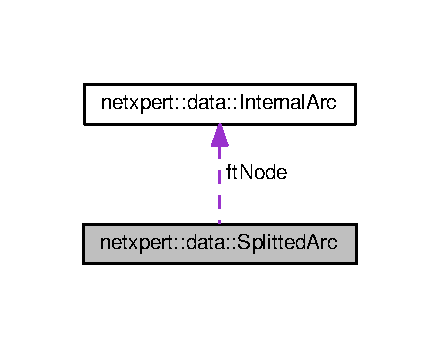
\includegraphics[width=211pt]{structnetxpert_1_1data_1_1SplittedArc__coll__graph}
\end{center}
\end{figure}
\subsection*{Public Attributes}
\begin{DoxyCompactItemize}
\item 
\hyperlink{structnetxpert_1_1data_1_1InternalArc}{netxpert\+::data\+::\+Internal\+Arc} {\bfseries ft\+Node}\hypertarget{structnetxpert_1_1data_1_1SplittedArc_a3aace0faa1861aa73cc19e8d09c9fb3c}{}\label{structnetxpert_1_1data_1_1SplittedArc_a3aace0faa1861aa73cc19e8d09c9fb3c}

\item 
cost\+\_\+t {\bfseries cost}\hypertarget{structnetxpert_1_1data_1_1SplittedArc_a8ec0717b28129abacfcf18c4c3895865}{}\label{structnetxpert_1_1data_1_1SplittedArc_a8ec0717b28129abacfcf18c4c3895865}

\item 
capacity\+\_\+t {\bfseries capacity}\hypertarget{structnetxpert_1_1data_1_1SplittedArc_a8b9bb43684e645f440c890783c8c0053}{}\label{structnetxpert_1_1data_1_1SplittedArc_a8b9bb43684e645f440c890783c8c0053}

\item 
std\+::shared\+\_\+ptr$<$ geos\+::geom\+::\+Multi\+Line\+String $>$ {\bfseries arc\+Geom}\hypertarget{structnetxpert_1_1data_1_1SplittedArc_ae8523bb6a235e0b448e80dbb91f182b0}{}\label{structnetxpert_1_1data_1_1SplittedArc_ae8523bb6a235e0b448e80dbb91f182b0}

\end{DoxyCompactItemize}


\subsection{Detailed Description}
Data type for storing tuple $<$from\+Node,to\+Node,arc\+Geom,cost,capacity$>$ 

The documentation for this struct was generated from the following file\+:\begin{DoxyCompactItemize}
\item 
/home/hahne/dev/netxpert1\+\_\+0/include/data.\+h\end{DoxyCompactItemize}

\hypertarget{classnetxpert_1_1core_1_1SPT__LEM}{}\section{netxpert\+:\+:core\+:\+:S\+P\+T\+\_\+\+L\+EM Class Reference}
\label{classnetxpert_1_1core_1_1SPT__LEM}\index{netxpert\+::core\+::\+S\+P\+T\+\_\+\+L\+EM@{netxpert\+::core\+::\+S\+P\+T\+\_\+\+L\+EM}}


Core Solver for the Shortest Path Tree Problem with binary Heap structure as default heap and Dijkstra\textquotesingle{}s algorithm of L\+E\+M\+ON.  




{\ttfamily \#include $<$sptlem.\+h$>$}



Inheritance diagram for netxpert\+:\+:core\+:\+:S\+P\+T\+\_\+\+L\+EM\+:\nopagebreak
\begin{figure}[H]
\begin{center}
\leavevmode
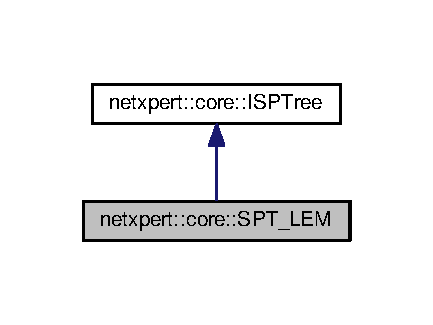
\includegraphics[width=208pt]{classnetxpert_1_1core_1_1SPT__LEM__inherit__graph}
\end{center}
\end{figure}


Collaboration diagram for netxpert\+:\+:core\+:\+:S\+P\+T\+\_\+\+L\+EM\+:\nopagebreak
\begin{figure}[H]
\begin{center}
\leavevmode
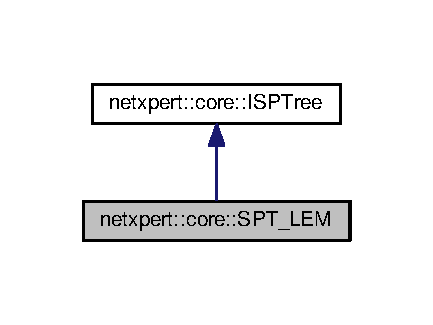
\includegraphics[width=208pt]{classnetxpert_1_1core_1_1SPT__LEM__coll__graph}
\end{center}
\end{figure}
\subsection*{Public Member Functions}
\begin{DoxyCompactItemize}
\item 
{\bfseries S\+P\+T\+\_\+\+L\+EM} (bool Drctd=true)\hypertarget{classnetxpert_1_1core_1_1SPT__LEM_ae8e11d1fcea636622f3c5d00e4642906}{}\label{classnetxpert_1_1core_1_1SPT__LEM_ae8e11d1fcea636622f3c5d00e4642906}

\item 
{\bfseries S\+P\+T\+\_\+\+L\+EM} (\hyperlink{classnetxpert_1_1core_1_1SPT__LEM}{S\+P\+T\+\_\+\+L\+EM} const \&)\hypertarget{classnetxpert_1_1core_1_1SPT__LEM_a1b1e3f1f5e6fb2a475395df5de1c8f7f}{}\label{classnetxpert_1_1core_1_1SPT__LEM_a1b1e3f1f5e6fb2a475395df5de1c8f7f}

\item 
void {\bfseries Load\+Net} (const uint32\+\_\+t nmax, const uint32\+\_\+t mmax, netxpert\+::data\+::filtered\+\_\+graph\+\_\+t $\ast$sg, netxpert\+::data\+::graph\+\_\+t\+::\+Arc\+Map$<$ netxpert\+::data\+::cost\+\_\+t $>$ $\ast$cm)\hypertarget{classnetxpert_1_1core_1_1SPT__LEM_a8fb936136e0c7e6c9f9e5eea9c7acba0}{}\label{classnetxpert_1_1core_1_1SPT__LEM_a8fb936136e0c7e6c9f9e5eea9c7acba0}

\item 
const uint32\+\_\+t {\bfseries Get\+Arc\+Count} ()\hypertarget{classnetxpert_1_1core_1_1SPT__LEM_acb011f54ba18bc9c5e2709129137fd72}{}\label{classnetxpert_1_1core_1_1SPT__LEM_acb011f54ba18bc9c5e2709129137fd72}

\item 
const uint32\+\_\+t {\bfseries Get\+Node\+Count} ()\hypertarget{classnetxpert_1_1core_1_1SPT__LEM_a15b68704ba3c584b3fbd66b283e54556}{}\label{classnetxpert_1_1core_1_1SPT__LEM_a15b68704ba3c584b3fbd66b283e54556}

\item 
void {\bfseries Solve\+S\+PT} (netxpert\+::data\+::cost\+\_\+t treshold=-\/1, bool bidirectional=true)\hypertarget{classnetxpert_1_1core_1_1SPT__LEM_a0baaa3bca3fbc8fcaeb97497735b0d93}{}\label{classnetxpert_1_1core_1_1SPT__LEM_a0baaa3bca3fbc8fcaeb97497735b0d93}

\item 
void {\bfseries Set\+Origin} (netxpert\+::data\+::node\+\_\+t \+\_\+origin)\hypertarget{classnetxpert_1_1core_1_1SPT__LEM_aacd93e8aa563539216b60b43c19871cc}{}\label{classnetxpert_1_1core_1_1SPT__LEM_aacd93e8aa563539216b60b43c19871cc}

\item 
void {\bfseries Set\+Dest} (netxpert\+::data\+::node\+\_\+t \+\_\+dest)\hypertarget{classnetxpert_1_1core_1_1SPT__LEM_a94de1da6ae4cc62cfb92d08b9f005912}{}\label{classnetxpert_1_1core_1_1SPT__LEM_a94de1da6ae4cc62cfb92d08b9f005912}

\item 
bool {\bfseries Reached} (netxpert\+::data\+::node\+\_\+t \+\_\+node)\hypertarget{classnetxpert_1_1core_1_1SPT__LEM_a13157e4e557cb7c8a4491855af49350b}{}\label{classnetxpert_1_1core_1_1SPT__LEM_a13157e4e557cb7c8a4491855af49350b}

\item 
const std\+::vector$<$ netxpert\+::data\+::node\+\_\+t $>$ {\bfseries Get\+Predecessors} (netxpert\+::data\+::node\+\_\+t \+\_\+dest)\hypertarget{classnetxpert_1_1core_1_1SPT__LEM_a86a2fd01219e9050743a704e932b1705}{}\label{classnetxpert_1_1core_1_1SPT__LEM_a86a2fd01219e9050743a704e932b1705}

\item 
const std\+::vector$<$ netxpert\+::data\+::arc\+\_\+t $>$ {\bfseries Get\+Path} (netxpert\+::data\+::node\+\_\+t \+\_\+dest)\hypertarget{classnetxpert_1_1core_1_1SPT__LEM_a716f3ddb0319ce581c903020d14a59db}{}\label{classnetxpert_1_1core_1_1SPT__LEM_a716f3ddb0319ce581c903020d14a59db}

\item 
const netxpert\+::data\+::cost\+\_\+t {\bfseries Get\+Dist} (netxpert\+::data\+::node\+\_\+t \+\_\+dest)\hypertarget{classnetxpert_1_1core_1_1SPT__LEM_a5b090847e90271c3dbc8215e37f642a7}{}\label{classnetxpert_1_1core_1_1SPT__LEM_a5b090847e90271c3dbc8215e37f642a7}

\end{DoxyCompactItemize}
\subsection*{Protected Attributes}
\begin{DoxyCompactItemize}
\item 
uint32\+\_\+t {\bfseries nmax}\hypertarget{classnetxpert_1_1core_1_1SPT__LEM_a8ded380546a1da7734d9ce23010a1cd9}{}\label{classnetxpert_1_1core_1_1SPT__LEM_a8ded380546a1da7734d9ce23010a1cd9}

\item 
uint32\+\_\+t {\bfseries mmax}\hypertarget{classnetxpert_1_1core_1_1SPT__LEM_a6ea75eb48f7f45bd19c4d126099e5dd9}{}\label{classnetxpert_1_1core_1_1SPT__LEM_a6ea75eb48f7f45bd19c4d126099e5dd9}

\end{DoxyCompactItemize}


\subsection{Detailed Description}
Core Solver for the Shortest Path Tree Problem with binary Heap structure as default heap and Dijkstra\textquotesingle{}s algorithm of L\+E\+M\+ON. 

The documentation for this class was generated from the following file\+:\begin{DoxyCompactItemize}
\item 
/home/hahne/dev/netxpert1\+\_\+0/include/core/sptlem.\+h\end{DoxyCompactItemize}

\hypertarget{structnetxpert_1_1data_1_1SPTResult}{}\section{netxpert\+:\+:data\+:\+:S\+P\+T\+Result Struct Reference}
\label{structnetxpert_1_1data_1_1SPTResult}\index{netxpert\+::data\+::\+S\+P\+T\+Result@{netxpert\+::data\+::\+S\+P\+T\+Result}}


Data type for storing the result of the S\+PT Solver in J\+S\+O\+N-\/\+Format.  




{\ttfamily \#include $<$data.\+h$>$}

\subsection*{Public Member Functions}
\begin{DoxyCompactItemize}
\item 
{\footnotesize template$<$class Archive $>$ }\\void {\bfseries serialize} (Archive \&ar)\hypertarget{structnetxpert_1_1data_1_1SPTResult_ac789313adfb3db98372f69d7e964a441}{}\label{structnetxpert_1_1data_1_1SPTResult_ac789313adfb3db98372f69d7e964a441}

\end{DoxyCompactItemize}
\subsection*{Public Attributes}
\begin{DoxyCompactItemize}
\item 
cost\+\_\+t {\bfseries optimum}\hypertarget{structnetxpert_1_1data_1_1SPTResult_a7474e0933e165b85736ae54482e91666}{}\label{structnetxpert_1_1data_1_1SPTResult_a7474e0933e165b85736ae54482e91666}

\item 
std\+::vector$<$ \hyperlink{structnetxpert_1_1data_1_1ExtSPTreeArc}{netxpert\+::data\+::\+Ext\+S\+P\+Tree\+Arc} $>$ {\bfseries spt}\hypertarget{structnetxpert_1_1data_1_1SPTResult_a7f5134ed3043eb8d93d8f2009bc58c2b}{}\label{structnetxpert_1_1data_1_1SPTResult_a7f5134ed3043eb8d93d8f2009bc58c2b}

\end{DoxyCompactItemize}


\subsection{Detailed Description}
Data type for storing the result of the S\+PT Solver in J\+S\+O\+N-\/\+Format. 

The documentation for this struct was generated from the following file\+:\begin{DoxyCompactItemize}
\item 
/home/hahne/dev/netxpert1\+\_\+0/include/data.\+h\end{DoxyCompactItemize}

\hypertarget{classnetxpert_1_1utils_1_1Stopwatch}{}\section{netxpert\+:\+:utils\+:\+:Stopwatch$<$ TimeT, ClockT, DurationT $>$ Class Template Reference}
\label{classnetxpert_1_1utils_1_1Stopwatch}\index{netxpert\+::utils\+::\+Stopwatch$<$ Time\+T, Clock\+T, Duration\+T $>$@{netxpert\+::utils\+::\+Stopwatch$<$ Time\+T, Clock\+T, Duration\+T $>$}}
\subsection*{Public Member Functions}
\begin{DoxyCompactItemize}
\item 
void {\bfseries start} ()\hypertarget{classnetxpert_1_1utils_1_1Stopwatch_aae232eaac691cd36eac325fed4df9fe0}{}\label{classnetxpert_1_1utils_1_1Stopwatch_aae232eaac691cd36eac325fed4df9fe0}

\item 
DurationT {\bfseries stop} ()\hypertarget{classnetxpert_1_1utils_1_1Stopwatch_a3cd4be178b032591a5763b892777f126}{}\label{classnetxpert_1_1utils_1_1Stopwatch_a3cd4be178b032591a5763b892777f126}

\item 
DurationT {\bfseries elapsed} ()\hypertarget{classnetxpert_1_1utils_1_1Stopwatch_ae7b8d9c8d437571277decfe68e9a5aac}{}\label{classnetxpert_1_1utils_1_1Stopwatch_ae7b8d9c8d437571277decfe68e9a5aac}

\end{DoxyCompactItemize}


The documentation for this class was generated from the following file\+:\begin{DoxyCompactItemize}
\item 
/home/hahne/dev/netxpert1\+\_\+0/include/utils.\+h\end{DoxyCompactItemize}

\hypertarget{structnetxpert_1_1data_1_1SwappedOldArc}{}\section{netxpert\+:\+:data\+:\+:Swapped\+Old\+Arc Struct Reference}
\label{structnetxpert_1_1data_1_1SwappedOldArc}\index{netxpert\+::data\+::\+Swapped\+Old\+Arc@{netxpert\+::data\+::\+Swapped\+Old\+Arc}}


Collaboration diagram for netxpert\+:\+:data\+:\+:Swapped\+Old\+Arc\+:\nopagebreak
\begin{figure}[H]
\begin{center}
\leavevmode
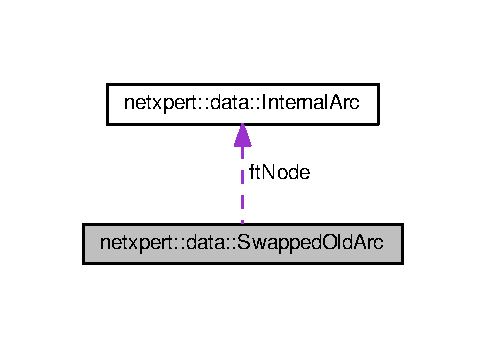
\includegraphics[width=233pt]{structnetxpert_1_1data_1_1SwappedOldArc__coll__graph}
\end{center}
\end{figure}
\subsection*{Public Attributes}
\begin{DoxyCompactItemize}
\item 
\hyperlink{structnetxpert_1_1data_1_1InternalArc}{netxpert\+::data\+::\+Internal\+Arc} {\bfseries ft\+Node}\hypertarget{structnetxpert_1_1data_1_1SwappedOldArc_aa3bb7dae740bf01acc60a9aec78d30ea}{}\label{structnetxpert_1_1data_1_1SwappedOldArc_aa3bb7dae740bf01acc60a9aec78d30ea}

\item 
cost\+\_\+t {\bfseries cost}\hypertarget{structnetxpert_1_1data_1_1SwappedOldArc_af6a61426c54e165ec413fc255c70f6df}{}\label{structnetxpert_1_1data_1_1SwappedOldArc_af6a61426c54e165ec413fc255c70f6df}

\item 
capacity\+\_\+t {\bfseries capacity}\hypertarget{structnetxpert_1_1data_1_1SwappedOldArc_a4fae66455a864ceb03224842df4210da}{}\label{structnetxpert_1_1data_1_1SwappedOldArc_a4fae66455a864ceb03224842df4210da}

\end{DoxyCompactItemize}


The documentation for this struct was generated from the following file\+:\begin{DoxyCompactItemize}
\item 
/home/hahne/dev/netxpert1\+\_\+0/include/data.\+h\end{DoxyCompactItemize}

\hypertarget{classnetxpert_1_1simple_1_1Transportation}{}\section{netxpert\+:\+:simple\+:\+:Transportation Class Reference}
\label{classnetxpert_1_1simple_1_1Transportation}\index{netxpert\+::simple\+::\+Transportation@{netxpert\+::simple\+::\+Transportation}}
\subsection*{Public Member Functions}
\begin{DoxyCompactItemize}
\item 
{\bfseries Transportation} (std\+::string json\+Cnfg)\hypertarget{classnetxpert_1_1simple_1_1Transportation_ad20d4fb083bca27030f954e7d38d90b6}{}\label{classnetxpert_1_1simple_1_1Transportation_ad20d4fb083bca27030f954e7d38d90b6}

\item 
int {\bfseries Solve} ()\hypertarget{classnetxpert_1_1simple_1_1Transportation_a6483918f2f94c48cf3157fdcf8656f0a}{}\label{classnetxpert_1_1simple_1_1Transportation_a6483918f2f94c48cf3157fdcf8656f0a}

\item 
double {\bfseries Get\+Optimum} ()\hypertarget{classnetxpert_1_1simple_1_1Transportation_a26f54056cff8ffdc19caa832354cde82}{}\label{classnetxpert_1_1simple_1_1Transportation_a26f54056cff8ffdc19caa832354cde82}

\item 
std\+::string {\bfseries Get\+Distribution\+As\+J\+S\+ON} ()\hypertarget{classnetxpert_1_1simple_1_1Transportation_a8ab271a28fbff93c6a95ed2a0442f619}{}\label{classnetxpert_1_1simple_1_1Transportation_a8ab271a28fbff93c6a95ed2a0442f619}

\item 
std\+::vector$<$ \hyperlink{structnetxpert_1_1data_1_1ExtDistributionArc}{netxpert\+::data\+::\+Ext\+Distribution\+Arc} $>$ {\bfseries Get\+Distribution} ()\hypertarget{classnetxpert_1_1simple_1_1Transportation_a03d1928b72bfab6ddc9514c23888a6b8}{}\label{classnetxpert_1_1simple_1_1Transportation_a03d1928b72bfab6ddc9514c23888a6b8}

\end{DoxyCompactItemize}


The documentation for this class was generated from the following file\+:\begin{DoxyCompactItemize}
\item 
/home/hahne/dev/netxpert1\+\_\+0/include/simple/transp\+\_\+simple.\+h\end{DoxyCompactItemize}

\hypertarget{classnetxpert_1_1Transportation}{}\section{netxpert\+:\+:Transportation Class Reference}
\label{classnetxpert_1_1Transportation}\index{netxpert\+::\+Transportation@{netxpert\+::\+Transportation}}


Solver for the \hyperlink{classnetxpert_1_1Transportation}{Transportation} Problem.  




{\ttfamily \#include $<$transportation.\+h$>$}



Inheritance diagram for netxpert\+:\+:Transportation\+:\nopagebreak
\begin{figure}[H]
\begin{center}
\leavevmode
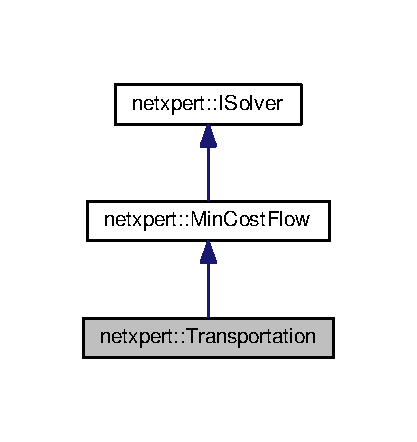
\includegraphics[width=200pt]{classnetxpert_1_1Transportation__inherit__graph}
\end{center}
\end{figure}


Collaboration diagram for netxpert\+:\+:Transportation\+:\nopagebreak
\begin{figure}[H]
\begin{center}
\leavevmode
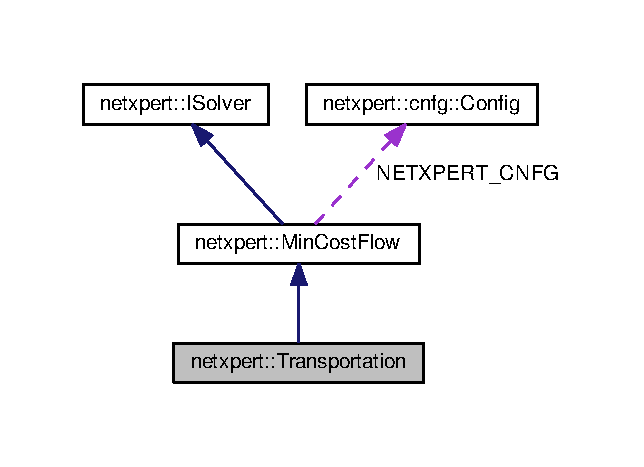
\includegraphics[width=309pt]{classnetxpert_1_1Transportation__coll__graph}
\end{center}
\end{figure}
\subsection*{Public Member Functions}
\begin{DoxyCompactItemize}
\item 
{\bfseries Transportation} (\hyperlink{structnetxpert_1_1cnfg_1_1Config}{netxpert\+::cnfg\+::\+Config} \&cnfg)\hypertarget{classnetxpert_1_1Transportation_ae6be3241f69bab69b2a1059178ae9fe5}{}\label{classnetxpert_1_1Transportation_ae6be3241f69bab69b2a1059178ae9fe5}

\item 
void {\bfseries Set\+Origins} (std\+::vector$<$ netxpert\+::data\+::node\+\_\+t $>$ \&origs)\hypertarget{classnetxpert_1_1Transportation_a89c684ee01d1ec1e3e02342cdc761837}{}\label{classnetxpert_1_1Transportation_a89c684ee01d1ec1e3e02342cdc761837}

\item 
void \hyperlink{classnetxpert_1_1Transportation_af603fe6fe78c175e90c002cec25c4f04}{Set\+Origins} (const std\+::vector$<$ uint32\+\_\+t $>$ \&origs)
\item 
std\+::vector$<$ netxpert\+::data\+::node\+\_\+t $>$ {\bfseries Get\+Origins} () const \hypertarget{classnetxpert_1_1Transportation_a5a6a99c1757a99e4dfa3fc1cd6f68f4f}{}\label{classnetxpert_1_1Transportation_a5a6a99c1757a99e4dfa3fc1cd6f68f4f}

\item 
std\+::vector$<$ uint32\+\_\+t $>$ \hyperlink{classnetxpert_1_1Transportation_afa07a6327889540be7db46ade38160f4}{Get\+Origin\+I\+Ds} () const 
\item 
void {\bfseries Set\+Destinations} (std\+::vector$<$ netxpert\+::data\+::node\+\_\+t $>$ \&dests)\hypertarget{classnetxpert_1_1Transportation_a8bfe70ee838457b6f25eb77de12c9ff2}{}\label{classnetxpert_1_1Transportation_a8bfe70ee838457b6f25eb77de12c9ff2}

\item 
void \hyperlink{classnetxpert_1_1Transportation_ac57b4230b6b295940fd673baa3b58c16}{Set\+Destinations} (const std\+::vector$<$ uint32\+\_\+t $>$ \&dests)
\item 
std\+::vector$<$ netxpert\+::data\+::node\+\_\+t $>$ {\bfseries Get\+Destinations} () const \hypertarget{classnetxpert_1_1Transportation_a9cb96d2c88207ef4599088f6562300dc}{}\label{classnetxpert_1_1Transportation_a9cb96d2c88207ef4599088f6562300dc}

\item 
std\+::vector$<$ uint32\+\_\+t $>$ \hyperlink{classnetxpert_1_1Transportation_ae901ff6721689f44d65373e79bc169b2}{Get\+Destination\+I\+Ds} () const 
\item 
void {\bfseries Set\+Ext\+O\+D\+Matrix} (std\+::vector$<$ \hyperlink{structnetxpert_1_1data_1_1ExtSPTreeArc}{netxpert\+::data\+::\+Ext\+S\+P\+Tree\+Arc} $>$ \+\_\+ext\+O\+D\+Matrix)\hypertarget{classnetxpert_1_1Transportation_aa3f6586670404e4c156afcd7ea1f6b3e}{}\label{classnetxpert_1_1Transportation_aa3f6586670404e4c156afcd7ea1f6b3e}

\item 
\hyperlink{classnetxpert_1_1InternalNet}{netxpert\+::\+Internal\+Net} $\ast$ {\bfseries Get\+Network} ()\hypertarget{classnetxpert_1_1Transportation_a404f8bbde60346861a1885b43a591ba8}{}\label{classnetxpert_1_1Transportation_a404f8bbde60346861a1885b43a591ba8}

\item 
void {\bfseries Set\+Ext\+Node\+Supply} (std\+::vector$<$ \hyperlink{structnetxpert_1_1data_1_1ExtNodeSupply}{netxpert\+::data\+::\+Ext\+Node\+Supply} $>$ \+\_\+node\+Supply)\hypertarget{classnetxpert_1_1Transportation_aba71c269cb507ee1575b203c13fe7898}{}\label{classnetxpert_1_1Transportation_aba71c269cb507ee1575b203c13fe7898}

\item 
std\+::map$<$ \hyperlink{structnetxpert_1_1data_1_1ODPair}{netxpert\+::data\+::\+O\+D\+Pair}, \hyperlink{structnetxpert_1_1data_1_1DistributionArc}{netxpert\+::data\+::\+Distribution\+Arc} $>$ {\bfseries Get\+Distribution} () const \hypertarget{classnetxpert_1_1Transportation_a937b20ec0d347a9950d272b931d1a312}{}\label{classnetxpert_1_1Transportation_a937b20ec0d347a9950d272b931d1a312}

\item 
std\+::string {\bfseries Get\+Solver\+J\+S\+O\+N\+Result} () const \hypertarget{classnetxpert_1_1Transportation_a8f902b10f9b0577029a125177c428f3c}{}\label{classnetxpert_1_1Transportation_a8f902b10f9b0577029a125177c428f3c}

\item 
std\+::vector$<$ \hyperlink{structnetxpert_1_1data_1_1ExtDistributionArc}{netxpert\+::data\+::\+Ext\+Distribution\+Arc} $>$ {\bfseries Get\+Ext\+Distribution} () const \hypertarget{classnetxpert_1_1Transportation_a53c91ad46f2ed5e2f2505d1a3d3c07fb}{}\label{classnetxpert_1_1Transportation_a53c91ad46f2ed5e2f2505d1a3d3c07fb}

\item 
std\+::string {\bfseries Get\+J\+S\+O\+N\+Ext\+Distribution} () const \hypertarget{classnetxpert_1_1Transportation_a3d7ada6b7c52f0c7e0ecf7cd4d795ff5}{}\label{classnetxpert_1_1Transportation_a3d7ada6b7c52f0c7e0ecf7cd4d795ff5}

\item 
void {\bfseries Save\+Results} (const std\+::string \&result\+Table\+Name, const \hyperlink{structnetxpert_1_1data_1_1ColumnMap}{netxpert\+::data\+::\+Column\+Map} \&cmap) const \hypertarget{classnetxpert_1_1Transportation_a5d79b20079a47ea164b692c7f2eed669}{}\label{classnetxpert_1_1Transportation_a5d79b20079a47ea164b692c7f2eed669}

\item 
void \hyperlink{classnetxpert_1_1Transportation_ac8b5f46f7332efb23cf4ef7add462b2b}{Solve} ()
\item 
void \hyperlink{classnetxpert_1_1Transportation_ada422481bba50b142ea0a5a73c29d276}{Solve} (\hyperlink{classnetxpert_1_1InternalNet}{netxpert\+::\+Internal\+Net} \&net)
\end{DoxyCompactItemize}
\subsection*{Additional Inherited Members}


\subsection{Detailed Description}
Solver for the \hyperlink{classnetxpert_1_1Transportation}{Transportation} Problem. 

\subsection{Member Function Documentation}
\index{netxpert\+::\+Transportation@{netxpert\+::\+Transportation}!Get\+Destination\+I\+Ds@{Get\+Destination\+I\+Ds}}
\index{Get\+Destination\+I\+Ds@{Get\+Destination\+I\+Ds}!netxpert\+::\+Transportation@{netxpert\+::\+Transportation}}
\subsubsection[{\texorpdfstring{Get\+Destination\+I\+Ds() const }{GetDestinationIDs() const }}]{\setlength{\rightskip}{0pt plus 5cm}std\+::vector$<$uint32\+\_\+t$>$ netxpert\+::\+Transportation\+::\+Get\+Destination\+I\+Ds (
\begin{DoxyParamCaption}
{}
\end{DoxyParamCaption}
) const\hspace{0.3cm}{\ttfamily [inline]}}\hypertarget{classnetxpert_1_1Transportation_ae901ff6721689f44d65373e79bc169b2}{}\label{classnetxpert_1_1Transportation_ae901ff6721689f44d65373e79bc169b2}
Simple Wrapper for S\+W\+IG \index{netxpert\+::\+Transportation@{netxpert\+::\+Transportation}!Get\+Origin\+I\+Ds@{Get\+Origin\+I\+Ds}}
\index{Get\+Origin\+I\+Ds@{Get\+Origin\+I\+Ds}!netxpert\+::\+Transportation@{netxpert\+::\+Transportation}}
\subsubsection[{\texorpdfstring{Get\+Origin\+I\+Ds() const }{GetOriginIDs() const }}]{\setlength{\rightskip}{0pt plus 5cm}std\+::vector$<$uint32\+\_\+t$>$ netxpert\+::\+Transportation\+::\+Get\+Origin\+I\+Ds (
\begin{DoxyParamCaption}
{}
\end{DoxyParamCaption}
) const\hspace{0.3cm}{\ttfamily [inline]}}\hypertarget{classnetxpert_1_1Transportation_afa07a6327889540be7db46ade38160f4}{}\label{classnetxpert_1_1Transportation_afa07a6327889540be7db46ade38160f4}
Simple Wrapper for S\+W\+IG \index{netxpert\+::\+Transportation@{netxpert\+::\+Transportation}!Set\+Destinations@{Set\+Destinations}}
\index{Set\+Destinations@{Set\+Destinations}!netxpert\+::\+Transportation@{netxpert\+::\+Transportation}}
\subsubsection[{\texorpdfstring{Set\+Destinations(const std\+::vector$<$ uint32\+\_\+t $>$ \&dests)}{SetDestinations(const std::vector< uint32_t > &dests)}}]{\setlength{\rightskip}{0pt plus 5cm}void netxpert\+::\+Transportation\+::\+Set\+Destinations (
\begin{DoxyParamCaption}
\item[{const std\+::vector$<$ uint32\+\_\+t $>$ \&}]{dests}
\end{DoxyParamCaption}
)\hspace{0.3cm}{\ttfamily [inline]}}\hypertarget{classnetxpert_1_1Transportation_ac57b4230b6b295940fd673baa3b58c16}{}\label{classnetxpert_1_1Transportation_ac57b4230b6b295940fd673baa3b58c16}
Simple Wrapper for S\+W\+IG \index{netxpert\+::\+Transportation@{netxpert\+::\+Transportation}!Set\+Origins@{Set\+Origins}}
\index{Set\+Origins@{Set\+Origins}!netxpert\+::\+Transportation@{netxpert\+::\+Transportation}}
\subsubsection[{\texorpdfstring{Set\+Origins(const std\+::vector$<$ uint32\+\_\+t $>$ \&origs)}{SetOrigins(const std::vector< uint32_t > &origs)}}]{\setlength{\rightskip}{0pt plus 5cm}void netxpert\+::\+Transportation\+::\+Set\+Origins (
\begin{DoxyParamCaption}
\item[{const std\+::vector$<$ uint32\+\_\+t $>$ \&}]{origs}
\end{DoxyParamCaption}
)\hspace{0.3cm}{\ttfamily [inline]}}\hypertarget{classnetxpert_1_1Transportation_af603fe6fe78c175e90c002cec25c4f04}{}\label{classnetxpert_1_1Transportation_af603fe6fe78c175e90c002cec25c4f04}
Simple Wrapper for S\+W\+IG \index{netxpert\+::\+Transportation@{netxpert\+::\+Transportation}!Solve@{Solve}}
\index{Solve@{Solve}!netxpert\+::\+Transportation@{netxpert\+::\+Transportation}}
\subsubsection[{\texorpdfstring{Solve()}{Solve()}}]{\setlength{\rightskip}{0pt plus 5cm}void netxpert\+::\+Transportation\+::\+Solve (
\begin{DoxyParamCaption}
{}
\end{DoxyParamCaption}
)}\hypertarget{classnetxpert_1_1Transportation_ac8b5f46f7332efb23cf4ef7add462b2b}{}\label{classnetxpert_1_1Transportation_ac8b5f46f7332efb23cf4ef7add462b2b}
Solves the \hyperlink{classnetxpert_1_1Transportation}{Transportation} Problem with the defined O\+D\+Matrix and Node\+Supply property. Solves on pure attribute data only i.\+e. output is always without geometry. (G\+E\+O\+M\+E\+T\+R\+Y\+\_\+\+H\+A\+N\+D\+L\+I\+NG is always set to \char`\"{}\+No\+Geometry\char`\"{}) \index{netxpert\+::\+Transportation@{netxpert\+::\+Transportation}!Solve@{Solve}}
\index{Solve@{Solve}!netxpert\+::\+Transportation@{netxpert\+::\+Transportation}}
\subsubsection[{\texorpdfstring{Solve(netxpert\+::\+Internal\+Net \&net)}{Solve(netxpert::InternalNet &net)}}]{\setlength{\rightskip}{0pt plus 5cm}void netxpert\+::\+Transportation\+::\+Solve (
\begin{DoxyParamCaption}
\item[{{\bf netxpert\+::\+Internal\+Net} \&}]{net}
\end{DoxyParamCaption}
)\hspace{0.3cm}{\ttfamily [virtual]}}\hypertarget{classnetxpert_1_1Transportation_ada422481bba50b142ea0a5a73c29d276}{}\label{classnetxpert_1_1Transportation_ada422481bba50b142ea0a5a73c29d276}
Solves the \hyperlink{classnetxpert_1_1Transportation}{Transportation} Problem with the given network and all origin and destination nodes. Uses the Net\+Xpert \hyperlink{classnetxpert_1_1OriginDestinationMatrix}{Origin\+Destination\+Matrix} Solver internally. 

Reimplemented from \hyperlink{classnetxpert_1_1MinCostFlow}{netxpert\+::\+Min\+Cost\+Flow}.



The documentation for this class was generated from the following file\+:\begin{DoxyCompactItemize}
\item 
/home/hahne/dev/netxpert1\+\_\+0/include/solver/transportation.\+h\end{DoxyCompactItemize}

\hypertarget{structnetxpert_1_1data_1_1TransportationResult}{}\section{netxpert\+:\+:data\+:\+:Transportation\+Result Struct Reference}
\label{structnetxpert_1_1data_1_1TransportationResult}\index{netxpert\+::data\+::\+Transportation\+Result@{netxpert\+::data\+::\+Transportation\+Result}}


Data type for storing the result of the Transpotation Solver in J\+S\+O\+N-\/\+Format.  




{\ttfamily \#include $<$data.\+h$>$}

\subsection*{Public Member Functions}
\begin{DoxyCompactItemize}
\item 
{\footnotesize template$<$class Archive $>$ }\\void {\bfseries serialize} (Archive \&ar)\hypertarget{structnetxpert_1_1data_1_1TransportationResult_a688ff859e14c24d46073b256fba0b91d}{}\label{structnetxpert_1_1data_1_1TransportationResult_a688ff859e14c24d46073b256fba0b91d}

\end{DoxyCompactItemize}
\subsection*{Public Attributes}
\begin{DoxyCompactItemize}
\item 
cost\+\_\+t {\bfseries optimum}\hypertarget{structnetxpert_1_1data_1_1TransportationResult_a2e3f7cdd01d4e888ddbd977fcd2568f1}{}\label{structnetxpert_1_1data_1_1TransportationResult_a2e3f7cdd01d4e888ddbd977fcd2568f1}

\item 
std\+::vector$<$ \hyperlink{structnetxpert_1_1data_1_1ExtDistributionArc}{netxpert\+::data\+::\+Ext\+Distribution\+Arc} $>$ {\bfseries dist}\hypertarget{structnetxpert_1_1data_1_1TransportationResult_a6308fdc81da323f01a7a650d7f86c772}{}\label{structnetxpert_1_1data_1_1TransportationResult_a6308fdc81da323f01a7a650d7f86c772}

\end{DoxyCompactItemize}


\subsection{Detailed Description}
Data type for storing the result of the Transpotation Solver in J\+S\+O\+N-\/\+Format. 

The documentation for this struct was generated from the following file\+:\begin{DoxyCompactItemize}
\item 
/home/hahne/dev/netxpert1\+\_\+0/include/data.\+h\end{DoxyCompactItemize}

\hypertarget{classnetxpert_1_1utils_1_1UTILS}{}\section{netxpert\+:\+:utils\+:\+:U\+T\+I\+LS Class Reference}
\label{classnetxpert_1_1utils_1_1UTILS}\index{netxpert\+::utils\+::\+U\+T\+I\+LS@{netxpert\+::utils\+::\+U\+T\+I\+LS}}


{\ttfamily \#include $<$utils.\+h$>$}

\subsection*{Static Public Member Functions}
\begin{DoxyCompactItemize}
\item 
static bool {\bfseries Path\+Exists} (const std\+::string \&path)\hypertarget{classnetxpert_1_1utils_1_1UTILS_a3ec5804a79dca438bcc2eba9724a1cee}{}\label{classnetxpert_1_1utils_1_1UTILS_a3ec5804a79dca438bcc2eba9724a1cee}

\item 
static bool {\bfseries File\+Exists} (const std\+::string \&path)\hypertarget{classnetxpert_1_1utils_1_1UTILS_a143eeceead6be450b106f5b1f7f21323}{}\label{classnetxpert_1_1utils_1_1UTILS_a143eeceead6be450b106f5b1f7f21323}

\item 
static std\+::string {\bfseries Get\+Current\+Dir} ()\hypertarget{classnetxpert_1_1utils_1_1UTILS_a820571660f5778938e6a6763f338bb13}{}\label{classnetxpert_1_1utils_1_1UTILS_a820571660f5778938e6a6763f338bb13}

\item 
static bool {\bfseries Set\+Current\+Dir} (const std\+::string \&path)\hypertarget{classnetxpert_1_1utils_1_1UTILS_ac2f7d62ac547561bd266f70f59b31711}{}\label{classnetxpert_1_1utils_1_1UTILS_ac2f7d62ac547561bd266f70f59b31711}

\item 
static std\+::string {\bfseries Get\+Directory\+Name} (std\+::string \&\+\_\+file\+Path)\hypertarget{classnetxpert_1_1utils_1_1UTILS_ae3d6a8e0da3d811b2c2c715b36420b67}{}\label{classnetxpert_1_1utils_1_1UTILS_ae3d6a8e0da3d811b2c2c715b36420b67}

\item 
static std\+::string {\bfseries Get\+File\+Name\+Without\+Extension} (std\+::string \&\+\_\+file\+Path)\hypertarget{classnetxpert_1_1utils_1_1UTILS_ae95928fe63cac5d7c15b8b47d40e3633}{}\label{classnetxpert_1_1utils_1_1UTILS_ae95928fe63cac5d7c15b8b47d40e3633}

\item 
static std\+::vector$<$ std\+::string $>$ \& {\bfseries Split} (const std\+::string \&s, char delim, std\+::vector$<$ std\+::string $>$ \&elems)\hypertarget{classnetxpert_1_1utils_1_1UTILS_a6de9d330b1ba37ee4f00d1229bd3f2b1}{}\label{classnetxpert_1_1utils_1_1UTILS_a6de9d330b1ba37ee4f00d1229bd3f2b1}

\item 
static std\+::vector$<$ std\+::string $>$ {\bfseries Split} (const std\+::string \&s, char delim)\hypertarget{classnetxpert_1_1utils_1_1UTILS_a0024bea6b90e82c85e436ca366ab54c6}{}\label{classnetxpert_1_1utils_1_1UTILS_a0024bea6b90e82c85e436ca366ab54c6}

\item 
{\footnotesize template$<$typename T $>$ }\\static T {\bfseries Deserialize\+J\+S\+O\+Nto\+Object} (std\+::string \+\_\+json\+String)\hypertarget{classnetxpert_1_1utils_1_1UTILS_a48e234571d9187affb93de9fd137bec4}{}\label{classnetxpert_1_1utils_1_1UTILS_a48e234571d9187affb93de9fd137bec4}

\item 
{\footnotesize template$<$typename T $>$ }\\static std\+::string {\bfseries Serialize\+Object\+To\+J\+S\+ON} (T \+\_\+in\+Data, std\+::string \+\_\+root\+Node\+Name=\char`\"{}input\char`\"{})\hypertarget{classnetxpert_1_1utils_1_1UTILS_a9b8ad3ed8655cc589d935d6a2f8b524a}{}\label{classnetxpert_1_1utils_1_1UTILS_a9b8ad3ed8655cc589d935d6a2f8b524a}

\item 
static std\+::wstring {\bfseries convert\+String\+To\+W\+String} (const std\+::string \&s)\hypertarget{classnetxpert_1_1utils_1_1UTILS_a8be364101776edd0371a6d1ac2990266}{}\label{classnetxpert_1_1utils_1_1UTILS_a8be364101776edd0371a6d1ac2990266}

\item 
static std\+::string {\bfseries convert\+W\+String\+To\+String} (const std\+::wstring \&ws)\hypertarget{classnetxpert_1_1utils_1_1UTILS_a7d704cac4e1cc8e025a1cf7f730d0f34}{}\label{classnetxpert_1_1utils_1_1UTILS_a7d704cac4e1cc8e025a1cf7f730d0f34}

\item 
static std\+::string {\bfseries Replace} (std\+::string \&str, const std\+::string \&from, const std\+::string \&to)\hypertarget{classnetxpert_1_1utils_1_1UTILS_ac027e782541fb700dd1bf8aa7c9283bd}{}\label{classnetxpert_1_1utils_1_1UTILS_ac027e782541fb700dd1bf8aa7c9283bd}

\item 
static std\+::string {\bfseries Replace\+All} (std\+::string \&str, const std\+::string \&from, const std\+::string \&to)\hypertarget{classnetxpert_1_1utils_1_1UTILS_ad13853eb638c1d33afbb7bcfee7a857b}{}\label{classnetxpert_1_1utils_1_1UTILS_ad13853eb638c1d33afbb7bcfee7a857b}

\item 
static bool {\bfseries Is\+Equal} (const std\+::string \&a, const std\+::string \&b)\hypertarget{classnetxpert_1_1utils_1_1UTILS_a72a08ffc285bfbccdcbb182b48ebb4f4}{}\label{classnetxpert_1_1utils_1_1UTILS_a72a08ffc285bfbccdcbb182b48ebb4f4}

\end{DoxyCompactItemize}


\subsection{Detailed Description}
Static \hyperlink{classClass}{Class} that provides utility functions 

The documentation for this class was generated from the following file\+:\begin{DoxyCompactItemize}
\item 
/home/hahne/dev/netxpert1\+\_\+0/include/utils.\+h\end{DoxyCompactItemize}

%--- End generated contents ---

% Index
\backmatter
\newpage
\phantomsection
\clearemptydoublepage
\addcontentsline{toc}{chapter}{Index}
\printindex

\end{document}
